%**************************************%
%* Generated from MathBook XML source *%
%*    on 2016-06-29T13:14:02-04:00    *%
%*                                    *%
%*   http://mathbook.pugetsound.edu   *%
%*                                    *%
%**************************************%
\documentclass[10pt,]{book}
%% Load geometry package to allow page margin adjustments
\usepackage{geometry}
\geometry{letterpaper,total={5.0in,9.0in}}
%% Custom Preamble Entries, early (use latex.preamble.early)
%% Inline math delimiters, \(, \), need to be robust
%% 2016-01-31:  latexrelease.sty  supersedes  fixltx2e.sty
%% If  latexrelease.sty  exists, bugfix is in kernel
%% If not, bugfix is in  fixltx2e.sty
%% See:  https://tug.org/TUGboat/tb36-3/tb114ltnews22.pdf
%% and read "Fewer fragile commands" in distribution's  latexchanges.pdf
\IfFileExists{latexrelease.sty}{}{\usepackage{fixltx2e}}
%% Page Layout Adjustments (latex.geometry)
%% For unicode character support, use the "xelatex" executable
%% If never using xelatex, the next three lines can be removed
\usepackage{ifxetex}
\ifxetex\usepackage{xltxtra}\fi
%% Symbols, align environment, bracket-matrix
\usepackage{amsmath}
\usepackage{amssymb}
%% allow more columns to a matrix
%% can make this even bigger by overriding with  latex.preamble.late  processing option
\setcounter{MaxMatrixCols}{30}
%% Semantic Macros
%% To preserve meaning in a LaTeX file
%% Only defined here if required in this document
%% Used for inline definitions of terms
\newcommand{\terminology}[1]{\textbf{#1}}
%% Subdivision Numbering, Chapters, Sections, Subsections, etc
%% Subdivision numbers may be turned off at some level ("depth")
%% A section *always* has depth 1, contrary to us counting from the document root
%% The latex default is 3.  If a larger number is present here, then
%% removing this command may make some cross-references ambiguous
%% The precursor variable $numbering-maxlevel is checked for consistency in the common XSL file
\setcounter{secnumdepth}{3}
%% Environments with amsthm package
%% Theorem-like environments in "plain" style, with or without proof
\usepackage{amsthm}
\theoremstyle{plain}
%% Numbering for Theorems, Conjectures, Examples, Figures, etc
%% Controlled by  numbering.theorems.level  processing parameter
%% Always need a theorem environment to set base numbering scheme
%% even if document has no theorems (but has other environments)
\newtheorem{theorem}{Theorem}[section]
%% Only variants actually used in document appear here
%% Style is like a theorem, and for statements without proofs
%% Numbering: all theorem-like numbered consecutively
%% i.e. Corollary 4.3 follows Theorem 4.2
%% Definition-like environments, normal text
%% Numbering is in sync with theorems, etc
\theoremstyle{definition}
\newtheorem{definition}[theorem]{Definition}
%% Remark-like environments, normal text
%% Numbering is in sync with theorems, etc
\theoremstyle{definition}
\newtheorem{remark}[theorem]{Remark}
%% Example-like environments, normal text
%% Numbering is in sync with theorems, etc
\theoremstyle{definition}
\newtheorem{example}[theorem]{Example}
%% Numbering for Projects (independent of others)
%% Controlled by  numbering.projects.level  processing parameter
%% Always need a project environment to set base numbering scheme
%% even if document has no projectss (but has other blocks)
\newtheorem{project}{Project}[section]
%% Project-like environments, normal text
\theoremstyle{definition}
\newtheorem{activity}[project]{Activity}
%% Miscellaneous environments, normal text
%% Numbering for inline exercises and lists is in sync with theorems, etc
\theoremstyle{definition}
\newtheorem{exercise}[theorem]{Exercise}
%% Localize LaTeX supplied names (possibly none)
\renewcommand*{\chaptername}{Chapter}
%% Equation Numbering
%% Controlled by  numbering.equations.level  processing parameter
\numberwithin{equation}{section}
%% For improved tables
\usepackage{array}
%% Some extra height on each row is desirable, especially with horizontal rules
%% Increment determined experimentally
\setlength{\extrarowheight}{0.2ex}
%% Define variable thickness horizontal rules, full and partial
%% Thicknesses are 0.03, 0.05, 0.08 in the  booktabs  package
\makeatletter
\newcommand{\hrulethin}  {\noalign{\hrule height 0.04em}}
\newcommand{\hrulemedium}{\noalign{\hrule height 0.07em}}
\newcommand{\hrulethick} {\noalign{\hrule height 0.11em}}
%% We preserve a copy of the \setlength package before other
%% packages (extpfeil) get a chance to load packages that redefine it
\let\oldsetlength\setlength
\newlength{\Oldarrayrulewidth}
\newcommand{\crulethin}[1]%
{\noalign{\global\oldsetlength{\Oldarrayrulewidth}{\arrayrulewidth}}%
\noalign{\global\oldsetlength{\arrayrulewidth}{0.04em}}\cline{#1}%
\noalign{\global\oldsetlength{\arrayrulewidth}{\Oldarrayrulewidth}}}%
\newcommand{\crulemedium}[1]%
{\noalign{\global\oldsetlength{\Oldarrayrulewidth}{\arrayrulewidth}}%
\noalign{\global\oldsetlength{\arrayrulewidth}{0.07em}}\cline{#1}%
\noalign{\global\oldsetlength{\arrayrulewidth}{\Oldarrayrulewidth}}}
\newcommand{\crulethick}[1]%
{\noalign{\global\oldsetlength{\Oldarrayrulewidth}{\arrayrulewidth}}%
\noalign{\global\oldsetlength{\arrayrulewidth}{0.11em}}\cline{#1}%
\noalign{\global\oldsetlength{\arrayrulewidth}{\Oldarrayrulewidth}}}
%% Single letter column specifiers defined via array package
\newcolumntype{A}{!{\vrule width 0.04em}}
\newcolumntype{B}{!{\vrule width 0.07em}}
\newcolumntype{C}{!{\vrule width 0.11em}}
\makeatother
\newcommand{\tablecelllines}[3]%
{\begin{tabular}[#2]{@{}#1@{}}#3\end{tabular}}
%% Figures, Tables, Listings, Floats
%% The [H]ere option of the float package fixes floats in-place,
%% in deference to web usage, where floats are totally irrelevant
%% We re/define the figure, table and listing environments, if used
%%   1) New mbxfigure and/or mbxtable environments are defined with float package
%%   2) Standard LaTeX environments redefined to use new environments
%%   3) Standard LaTeX environments redefined to step theorem counter
%%   4) Counter for new environments is set to the theorem counter before caption
%% You can remove all this figure/table setup, to restore standard LaTeX behavior
%% HOWEVER, numbering of figures/tables AND theorems/examples/remarks, etc
%% WILL ALL de-synchronize with the numbering in the HTML version
%% You can remove the [H] argument of the \newfloat command, to allow flotation and 
%% preserve numbering, BUT the numbering may then appear "out-of-order"
\usepackage{float}
\usepackage[bf]{caption} % http://tex.stackexchange.com/questions/95631/defining-a-new-type-of-floating-environment 
\usepackage{newfloat}
% Side-by-side elements need careful treatement for aligning captions, see: 
% http://tex.stackexchange.com/questions/230335/vertically-aligning-minipages-subfigures-and-subtables-not-with-baseline 
\usepackage{stackengine,ifthen}
\newcounter{figstack}
\newcounter{figindex}
\newlength\fight
\newcommand\pushValignCaptionBottom[5][b]{%
\stepcounter{figstack}%
\expandafter\def\csname %
figalign\romannumeral\value{figstack}\endcsname{#1}%
\expandafter\def\csname %
figtype\romannumeral\value{figstack}\endcsname{#2}%
\expandafter\def\csname %
figwd\romannumeral\value{figstack}\endcsname{#3}%
\expandafter\def\csname %
figcontent\romannumeral\value{figstack}\endcsname{#4}%
\expandafter\def\csname %
figcap\romannumeral\value{figstack}\endcsname{#5}%
\setbox0=\hbox{%
\begin{#2}{#3}#4\end{#2}}%
\ifdim\dimexpr\ht0+\dp0\relax>\fight\global\setlength{\fight}{%
\dimexpr\ht0+\dp0\relax}\fi%
}
\newcommand\popValignCaptionBottom{%
\setcounter{figindex}{0}%
\hfill%
\whiledo{\value{figindex}<\value{figstack}}{%
\stepcounter{figindex}%
\def\tmp{\csname figwd\romannumeral\value{figindex}\endcsname}%
\begin{\csname figtype\romannumeral\value{figindex}\endcsname}[t]{\tmp}%
\centering%
\stackinset{c}{}%
{\csname figalign\romannumeral\value{figindex}\endcsname}{}%
{\csname figcontent\romannumeral\value{figindex}\endcsname}%
{\rule{0pt}{\fight}}\par%
\csname figcap\romannumeral\value{figindex}\endcsname%
\end{\csname figtype\romannumeral\value{figindex}\endcsname}%
\hfill%
}%
\setcounter{figstack}{0}%
\setlength{\fight}{0pt}%
\hfill%
}
% Figure environment setup so that it no longer floats
\SetupFloatingEnvironment{figure}{fileext=lof,placement={H},within=section,name=Figure}
% figures have the same number as theorems: http://tex.stackexchange.com/questions/16195/how-to-make-equations-figures-and-theorems-use-the-same-numbering-scheme 
\makeatletter
\let\c@figure\c@theorem
\makeatother
% Table environment setup so that it no longer floats
\SetupFloatingEnvironment{table}{fileext=lot,placement={H},within=section,name=Table}
% tables have the same number as theorems: http://tex.stackexchange.com/questions/16195/how-to-make-equations-figures-and-theorems-use-the-same-numbering-scheme 
\makeatletter
\let\c@table\c@theorem
\makeatother
%% Raster graphics inclusion, wrapped figures in paragraphs
\usepackage{graphicx}
%% Colors for Sage boxes and author tools (red hilites)
\usepackage[usenames,dvipsnames,svgnames,table]{xcolor}
%% New typewriter font if  c, sage, program, console, pre  tags present
%% If only  email, url  tags, no change from default
%% Needs a bit of scaling down to match text
\usepackage[scaled=.95]{sourcecodepro}
%% Program listing support, for inline code, Sage code
\usepackage{listings}
%% We define the listings font style to be the default "ttfamily"
%% To fix hyphens/dashes rendered in PDF as fancy minus signs by listing
%% http://tex.stackexchange.com/questions/33185/listings-package-changes-hyphens-to-minus-signs
\makeatletter
\lst@CCPutMacro\lst@ProcessOther {"2D}{\lst@ttfamily{-{}}{-{}}}
\@empty\z@\@empty
\makeatother
%% End of generic listing adjustments
%% Inline code, typically from "c" element
%% Global, document-wide options apply to \lstinline
%% Search/replace \lstinline by \verb to remove this dependency
%% (redefining \lstinline with \verb is unlikely to work)
%% Also see "\renewcommand\UrlFont" below for matching font choice
\lstset{basicstyle=\small\ttfamily,breaklines=true,breakatwhitespace=true}
%% More flexible list management, esp. for references and exercises
%% But also for specifying labels (i.e. custom order) on nested lists
\usepackage{enumitem}
%% hyperref driver does not need to be specified
\usepackage{hyperref}
%% Hyperlinking active in PDFs, all links solid and blue
\hypersetup{colorlinks=true,linkcolor=blue,citecolor=blue,filecolor=blue,urlcolor=blue}
\hypersetup{pdftitle={Modeling, Functions, and Graphs}}
%% If you manually remove hyperref, leave in this next command
\providecommand\phantomsection{}
%% Use upright quotes rather than LaTeX's curly quotes
%% If custom font substitutions follow, this might be ineffective
%% If fonts lack upright quotes, the textcomp package is employed
\usepackage{upquote}
%% Graphics Preamble Entries
\usepackage{pgfplots}               % loads tikz package
\pgfplotsset{axis x line = middle,
             axis y line = middle}
\usetikzlibrary{backgrounds}
\usetikzlibrary{arrows,matrix}
%% If tikz has been loaded, replace ampersand with \amp macro
%% extpfeil package for certain extensible arrows,
%% as also provided by MathJax extension of the same name
%% NB: this package loads mtools, which loads calc, which redefines
%%     \setlength, so it can be removed if it seems to be in the 
%%     way and your math does not use:
%%     
%%     \xtwoheadrightarrow, \xtwoheadleftarrow, \xmapsto, \xlongequal, \xtofrom
%%     
%%     we have had to be extra careful with variable thickness
%%     lines in tables, and so also load this package late
\usepackage{extpfeil}
%% Custom Preamble Entries, late (use latex.preamble.late)
%% Begin: Author-provided macros
%% (From  docinfo/macros  element)
%% Plus three from MBX for XML characters
\newcommand{\alert}[1]{\mathbf{\color{magenta}{#1}}}
\delimitershortfall-1sp
\newcommand\abs[1]{\left|#1\right|}

\newcommand\degree[0]{^{\circ}}
\newcommand{\lt}{ < }
\newcommand{\gt}{ > }
\newcommand{\amp}{ & }
%% End: Author-provided macros
%% Title page information for book
\title{Modeling, Functions, and Graphs\\
{\large Algebra for College Students}}
\author{Katherine Yoshiwara\\
Department of Mathematics\\
Los Angeles Pierce College\\
\href{mailto:kyoshiwara@hotmail.com}{\nolinkurl{kyoshiwara@hotmail.com}}
}
\date{June 29, 2016}
\begin{document}
\frontmatter
%% begin: half-title
\thispagestyle{empty}
{\centering
\vspace*{0.28\textheight}
{\Huge Modeling, Functions, and Graphs}\\[2\baselineskip]
{\LARGE Algebra for College Students}\\
}
\clearpage
%% end:   half-title
%% begin: adcard
\thispagestyle{empty}
\null%
\clearpage
%% end:   adcard
%% begin: title page
%% Inspired by Peter Wilson's "titleDB" in "titlepages" CTAN package
\thispagestyle{empty}
{\centering
\vspace*{0.14\textheight}
{\Huge Modeling, Functions, and Graphs}\\[\baselineskip]
{\LARGE Algebra for College Students}\\[3\baselineskip]
{\Large Katherine Yoshiwara}\\[0.5\baselineskip]
{\Large Los Angeles Pierce College}\\[3\baselineskip]
{\Large June 29, 2016}\\}
\clearpage
%% end:   title page
%% begin: copyright-page
\thispagestyle{empty}
\noindent
Katherine Yoshiwara did her undergraduate work at Michigan State, her graduate work at UCLA, and retired from Los Angeles Pierce College.%
\par
She likes gardening.%
\par
\vspace*{\stretch{2}}
\noindent\textcopyright\ 2016\textendash{}2017\quad{}Katherine Yoshiwara\\[0.5\baselineskip]
Permission is granted to copy, distribute and/or modify this document under the terms of the GNU Free Documentation License, Version 1.2 or any later version published by the Free Software Foundation; with no Invariant Sections, no Front-Cover Texts, and no Back-Cover Texts.  A copy of the license is included in the appendix entitled ``GNU Free Documentation License.''  All trademarks\texttrademark{} are the registered\textregistered{} marks of their respective owners.\par
\vspace*{\stretch{1}}
\null\clearpage
%% end:   copyright-page
%% begin: acknowledgement
\chapter*{Acknowledgements}\label{acknowledgement-1}
\addcontentsline{toc}{chapter}{Acknowledgements}
I would like to thank my cats.%
\par
I would also like to acknowledge Bruce Yoshiwara for  helpful comments and suggestions. %
%% end:   acknowledgement
%% begin: preface
\chapter*{Preface}\label{preface-1}
\addcontentsline{toc}{chapter}{Preface}
Mathematics, as we all know, is the language of science, and fluency in algebraic skills has always been necessary for anyone aspiring to disciplines based on calculus. But in the information age, increasingly sophisticated mathematical methods are used in all fields of knowledge, from archaeology to zoology. Consequently, there is a new focus on the courses before calculus. The availability of calculators and computers allows students to tackle complex problems involving real data, but requires more attention to analysis and interpretation of results. All students, not just those headed for science and engineering, should develop a mathematical viewpoint, including critical thinking, problem-solving strategies, and estimation, in addition to computational skills. \emph{Modeling, Functions and Graphs} employs a variety of applications to motivate mathematical thinking.%
\typeout{************************************************}
\typeout{Section .1 MODELING}
\typeout{************************************************}
\section[MODELING]{MODELING}\label{section-1}
The ability to model problems or phenomena by algebraic expressions and equations is the ultimate goal of any algebra course. Through a variety of applications, we motivate students to develop the skills and techniques of algebra. Each chapter includes an interactive Investigation that gives students an opportunity to explore an openended modeling problem. These Investigations can be used in class as guided explorations or as projects for small groups. They are designed to show students how the mathematical techniques they are learning can be applied to study and understand new situations.%
\typeout{************************************************}
\typeout{Section .2 Functions}
\typeout{************************************************}
\section[Functions]{Functions}\label{section-2}
The fundamental concept underlying calculus and related disciplines is the notion of function, and students should acquire a good understanding of functions before they embark on their study of college-level mathematics. While the formal study of functions is usually the content of precalculus, it is not too early to begin building an intuitive understanding of functional relationships in the preceding algebra courses. These ideas are useful not only in calculus but in practically any field students may pursue. We begin working with functions in Chapter 1 and explore the different families of functions in subsequent chapters.%
\par
In all our work with functions and modeling we employ the “Rule of Four,” that all
problems should be considered using algebraic, numerical, graphical, and verbal methods.
It is the connections between these approaches that we have endeavored to establish in this course. At this level it is crucial that students learn to write an algebraic expression from a verbal description, recognize trends in a table of data, and
extract and interpret information from the graph of a function.%
\typeout{************************************************}
\typeout{Section .3 Graphs}
\typeout{************************************************}
\section[Graphs]{Graphs}\label{section-3}
No tool for conveying information about a system is more powerful than a graph. Yet many students have trouble progressing from a point-wise understanding of graphs to a more
global view. By taking advantage of graphing calculators, we examine a large number of examples and study them in more detail than is possible when every graph is plotted by hand. We can consider more realistic models in which calculations by more traditional methods are difficult or impossible.%
\par
We have incorporated graphing calculators into the text wherever they can be used to enhance understanding. Calculator use is not simply an add-on, but in many ways shapes
the organization of the material. The text includes instructions for the TI-84 graphing calculator, but these can easily be adapted to any other graphing utility. We have not attempted to use all the features of the calculator or to teach calculator use for its own sake, but in all cases have let the mathematics suggest how technology should be used.%
\par
%
\par\hfill\begin{tabular}{l@{}}
Katherine Yoshiwara\\
Atascadero, CA 2016
\end{tabular}\\\par
%% end:   preface
%% begin: preface
\chapter*{Contributors to the 5\(^\mathrm{th}\) Edition}\label{preface-2}
\addcontentsline{toc}{chapter}{Contributors to the 5\(^\mathrm{th}\) Edition}
\hypertarget{kyoshiwara}{}\noindent%
\parbox[t]{0.35\textwidth}{Katherine Yoshiwara}%
\parbox[t]{0.65\textwidth}{Emerita Professor of Mathematics\\Los Angeles Pierce College\\}\par
%% end:   preface
%% begin: table of contents
\setcounter{tocdepth}{1}
\renewcommand*\contentsname{Contents}
\tableofcontents
%% end:   table of contents
\mainmatter
\typeout{************************************************}
\typeout{Chapter 1 Functions and Their Graphs}
\typeout{************************************************}
\chapter[Functions and Their Graphs]{Functions and Their Graphs}\label{chap1}
\typeout{************************************************}
\typeout{Introduction  }
\typeout{************************************************}
\includegraphics[width=0.60\textwidth,]{images/fig1.pdf}%
\par
You may have heard that mathematics is the language of science.  In fact, professionals in nearly every discipline take advantage of mathematical methods to analyze data, identify trends, and predict the effects of change.  This process is called \terminology{mathematical modeling}.  A model is a simplified representation of reality that helps us understand a process or phenomenon.  Because it is a simplification, a model can never be completely accurate.  Instead, it should focus on those aspects of the real situation that will help us answer specific questions. Here is an example. %
\par
The world's population is growing at different rates in different nations.  Many factors, including economic and social forces, influence the birth rate.  Is there a connection between birth rates and education levels?  The figure shows the birth rate plotted against the female literacy rate in 148 countries.  Although the data points do not all lie precisely on a line, we see a generally decreasing trend:  the higher the literacy rate, the lower the birth rate.  The \terminology{regression line} provides a model for this trend, and a tool for analyzing the data.  In this chapter we study the properties of linear models and some techniques for fitting a linear model to data.%
\leavevmode%
\begin{figure}
\centering
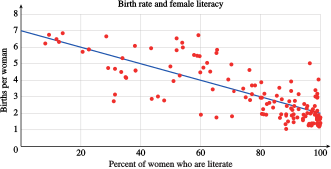
\includegraphics[width=0.100\textwidth,]{images/BirthRateVsFemaleLiteracy.pdf}\end{figure}
\typeout{************************************************}
\typeout{Paragraphs  Investigation: Sales on Commission}
\typeout{************************************************}
\paragraph[Investigation: Sales on Commission]{Investigation: Sales on Commission}\label{paragraphs-1}
Delbert is offered a part-time job selling restaurant equipment. He will be paid \textdollar{}1000 per month plus a 6\% commission on his sales. The sales manager tells Delbert he can expect to sell about \textdollar{}8000 worth of equipment per month. To help him decide whether to accept the job, Delbert does a few calculations.%
\par

                \leavevmode%
\begin{enumerate}
\item\hypertarget{li-1}{}Based on the sales manager’s estimate, what monthly income can Delbert expect from this job? What annual salary would that provide?%
\item\hypertarget{li-2}{}What would Delbert’s monthly salary be if he sold only \textdollar{}5000 of equipment per month? What would his salary be if he sold \textdollar{}10,000 worth per month? Compute monthly incomes for each sales total shown in the table.%
\leavevmode%
\begin{figure}
\centering
\pushValignCaptionBottom[b]{minipage}{.30\textwidth}{%
\centering% horizontal alignment 
\begin{tabular}{AcAcA}\hrulethick
Sales%
&Income%
\tabularnewline\hrulethin
5000&\tabularnewline\hrulethin
8000&\tabularnewline\hrulethin
10,000&\tabularnewline\hrulethin
12,000&\tabularnewline\hrulethin
15,000&\tabularnewline\hrulethin
18,000&\tabularnewline\hrulethin
20,000&\tabularnewline\hrulethin
25,000&\tabularnewline\hrulethin
30,000&\tabularnewline\hrulethin
35,000&\tabularnewline\hrulethin
~&\tabularnewline\hrulethin
~&\tabularnewline\hrulethin
\end{tabular}
}% end body 
{}% caption 
\pushValignCaptionBottom[b]{minipage}{.70\textwidth}{%
\centering% horizontal alignment 
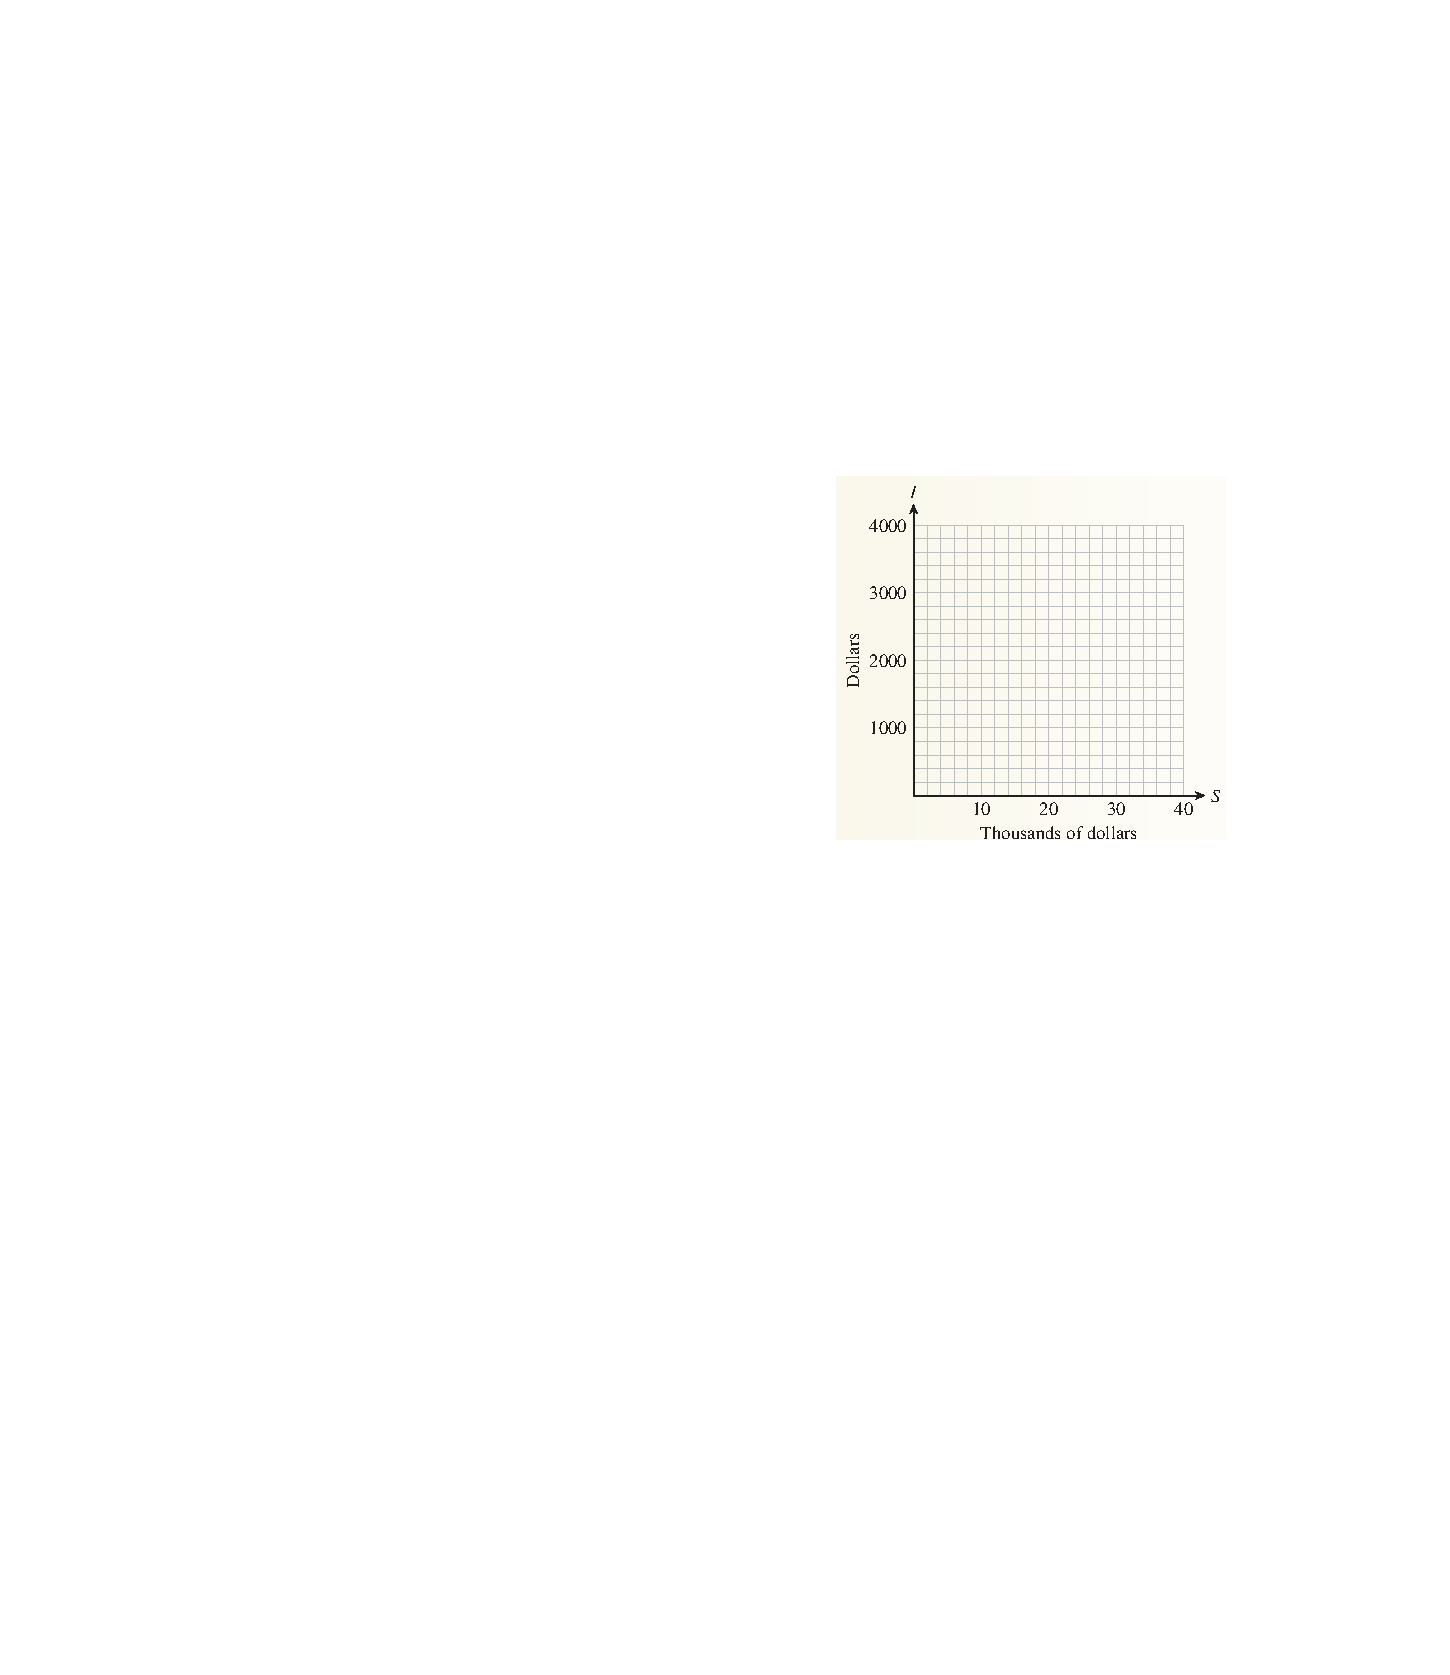
\includegraphics[width=\textwidth,]{images/Investigation1Grid.pdf}}% end body 
{}% caption 
\popValignCaptionBottom
\end{figure}
\item\hypertarget{li-3}{}Plot your data points on a graph, using sales, \(S\), on the horizontal axis and income, \(I\), on the vertical axis, as shown in the figure. Connect the data points to show Delbert’s monthly income for all possible monthly sales totals.%
\item\hypertarget{li-4}{} Add two new data points to the table by reading values from your graph.%
\item\hypertarget{li-5}{} Write an algebraic expression for Delbert’s monthly income, \(I\), in terms of his monthly sales, \(S\). Use the description in the problem to help you:%
\par

                    He will be paid: \textdollar{}1000 . . . plus a 6\% commission on his sales.%
\par
\emph{Income} \(=\)________________________ %
\item\hypertarget{li-6}{}Test your formula from part (5) to see if it gives the same results as those you recorded in the table.%
\item\hypertarget{li-7}{}Use your formula to find out what monthly sales total Delbert would need in order to have a monthly income of \textdollar{}2500.%
\item\hypertarget{li-8}{}Each increase of \textdollar{}1000 in monthly sales increases Delbert’s monthly income by ______________.%
\item\hypertarget{li-9}{}Summarize the results of your work: In your own words, describe the relationship between Delbert’s monthly sales and his monthly income. Include in your discussion a description of your graph.%
\end{enumerate}
%
\typeout{************************************************}
\typeout{Section 1.1 Linear Models}
\typeout{************************************************}
\section[Linear Models]{Linear Models}\label{LinMod}
\typeout{************************************************}
\typeout{Subsection 1.1.1 Tables, Graphs and Equations}
\typeout{************************************************}
\subsection[Tables, Graphs and Equations]{Tables, Graphs and Equations}\label{subsection-1}
The first step in creating a model is to describe relationships between variables.  In Investigation 1 {$\langle\langle$investigation-commission$\rangle\rangle$}, we analyzed the relationship between Delbert's sales and his income.  Starting from the verbal description of his income, we represented the relationship by a table of values, a graph, and an algebraic equation.  Each of these mathematical tools is useful in a different way.%
\leavevmode%
\begin{enumerate}
\item\hypertarget{li-10}{}A \terminology{table of values} displays specific data points with precise numerical values.%
\item\hypertarget{li-11}{}A \terminology{graph} is a visual display of the data.  It is easier to spot trends and describe the overall behavior of the variables from a graph.%
\item\hypertarget{li-12}{}An \terminology{algebraic equation} is a compact summary of the model.  It can be used to analyze the model and to make predictions%
\end{enumerate}
\par
We begin our study of modeling with some examples of \terminology{linear models}.  In the examples that follow, observe the interplay among the three modeling tools, and how each contributes to the model.%
\begin{example}[]\label{example-Annelise}
Annelise is on vacation at a seaside resort.  She can rent a bicycle from her hotel for \textdollar{}3 an hour, plus a \textdollar{}5 insurance fee.  (A fraction of an hour is charged as the same fraction of \textdollar{}3.)%
\leavevmode%
\begin{enumerate}[label=*\alph**]
\item\hypertarget{li-13}{}Make a table of values showing the cost, \(C\), of renting a bike for various lengths of time, \(t\).%
\item\hypertarget{li-14}{}Plot the points on a graph.  Draw a curve through the data points%
.
                        \item\hypertarget{li-15}{}Write an equation for \(C\) in terms of \(t\).%
\end{enumerate}
\par\medskip\noindent%
\textbf{Solution.}\quad \leavevmode%
\begin{enumerate}[label=*\alph**]
\item\hypertarget{li-16}{}To find the cost, multiply the time by \textdollar{}3, and add the result to the \textdollar{}5 insurance fee.  For example, the cost of a 1-hour bike ride is
                            \begin{align*}
\text{Cost}\amp=(\$5\text{ insurance fee})+(\$3\text{ per hour})\times(\alert{1}\text{ hour})\\
C\amp=5+3(\alert{1})=8
\end{align*}
                            A 1-hour bike ride costs \textdollar{}8.  Record the results in a table, as shown here:%
\leavevmode%
\begin{table}
\centering
\begin{tabular}{AcAcAcAcA}\hrulethick
Length of rental (hours)%
&Cost of rental (dollars)%
&&\((t,C)\)\tabularnewline\hrulethin
1&8&\(C=5+3(\alert{1})\)&\((1,8)\)\tabularnewline\hrulethin
2&11&\(C=5+3(\alert{2})\)&\((2,11)\)\tabularnewline\hrulethin
3&14&\(C=5+3(\alert{3})\)&\((3,14)\)\tabularnewline\hrulethin
\end{tabular}
\end{table}
\item\hypertarget{li-17}{}Each pair of values represents a point on the graph.  The first value gives the horizontal coordinate of the point, and the second value gives the vertical coordinate.  The points lie on a straight line, as shown in the figure.  The line extends infinitely in only one direction, because negative values of \(t\) do not make sense here.%
\leavevmode%
\begin{figure}
\centering
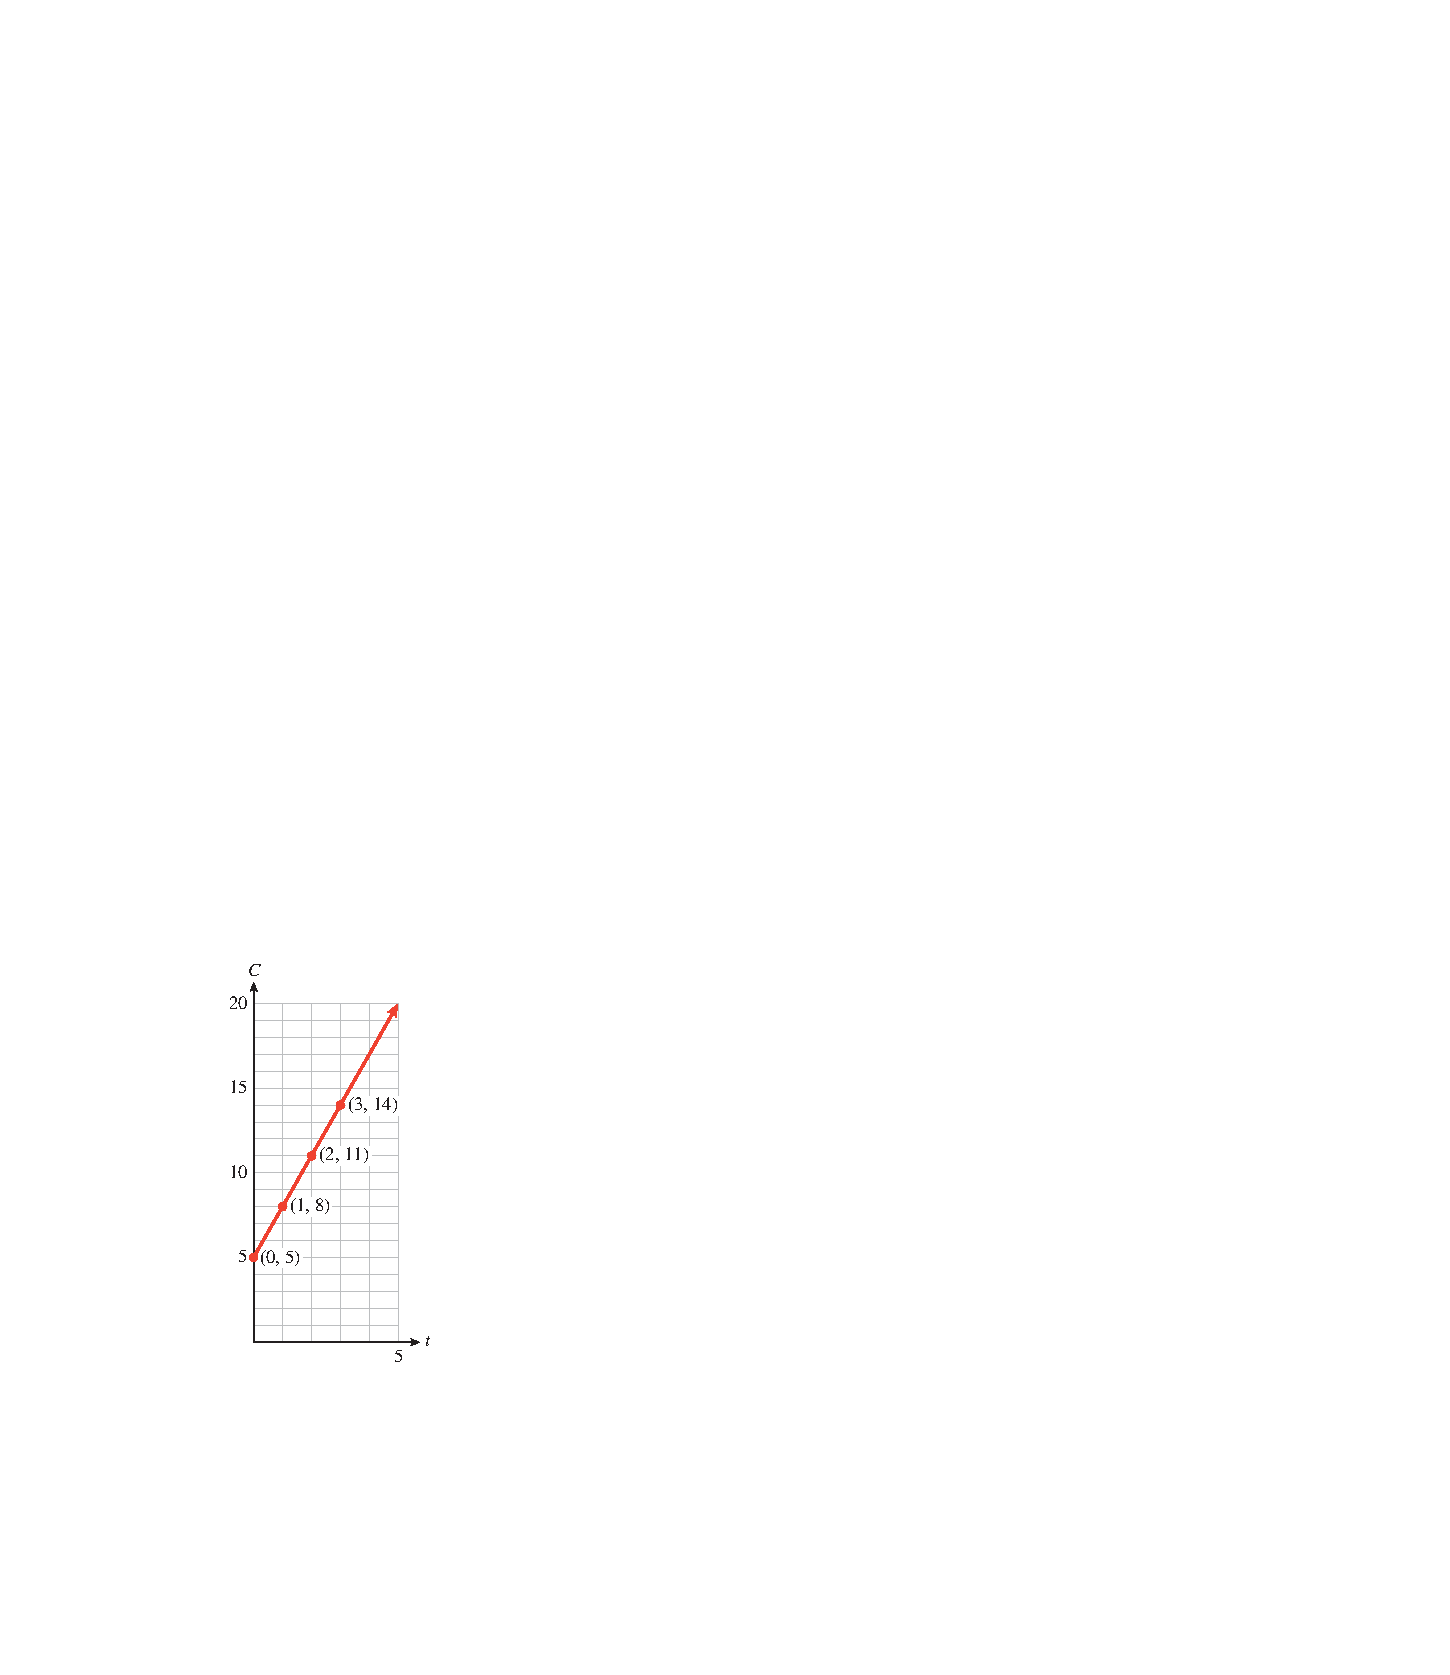
\includegraphics[width=0.50\textwidth,]{images/fig-Annelise-1.pdf}\end{figure}
\item\hypertarget{li-18}{}To find an equation, let \(C\) represent the cost of the rental, and use \(t\) for the number of hours:
        \begin{align*}
\text{Cost}\amp=(\$5\text{ insurance fee})+(\$3\text{ per hour})\times\text{(number of hours)}\\
C\amp=5+3\cdot t=8
\end{align*} %
\end{enumerate}
\end{example}
\begin{example}[]\label{example-6hrbike}
Use the equation \(C=5+3\cdot t\) you found in \hyperref[example-Annelise]{Example~\ref{example-Annelise}} to answer the following questions.  Then show how to find the answers by using the graph.%
\leavevmode%
\begin{enumerate}[label=*\alph**]
\item\hypertarget{li-19}{}How much will it cost Annelise to rent a bicycle for 6 hours?%
\item\hypertarget{li-20}{}How long can Annelise bicycle for \textdollar{}18.50?%
\end{enumerate}
\par\medskip\noindent%
\textbf{Solution.}\quad \leavevmode%
\begin{enumerate}[label=*\alph**]
\item\hypertarget{li-21}{}Substitute \(t=\alert{6}\) into the expression for \(C\) to find \begin{equation*}C=5+3(\alert{6})=23\end{equation*}A 6-hour bike ride will cost \textdollar{}23.  The point \(P\) on the graph in the figure represents the cost of a 6-hour bike ride.  The value on the \(C\)-axis at the same height as point \(P\) is 23, so a 6-hour bike ride costs \textdollar{}23.%
\item\hypertarget{li-22}{}Substitute \(C=\alert{18.50}\) into the equation and solve for \(t\).
        \begin{align*}
\alert{18.50}\amp=5+3t\\
13.50\amp=3t\\
t\amp=4.5
\end{align*}
        For \textdollar{}18.50 Annelise can bicycle for 4½ hours. The point \(Q\)  on the graph represents an \textdollar{}18.50 bike ride.  The value on the \(t\)-axis below point \(Q\) is 4.5, so \textdollar{}18.50 will buy a 4.5 hour bike ride.%
\end{enumerate}
\leavevmode%
\begin{figure}
\centering
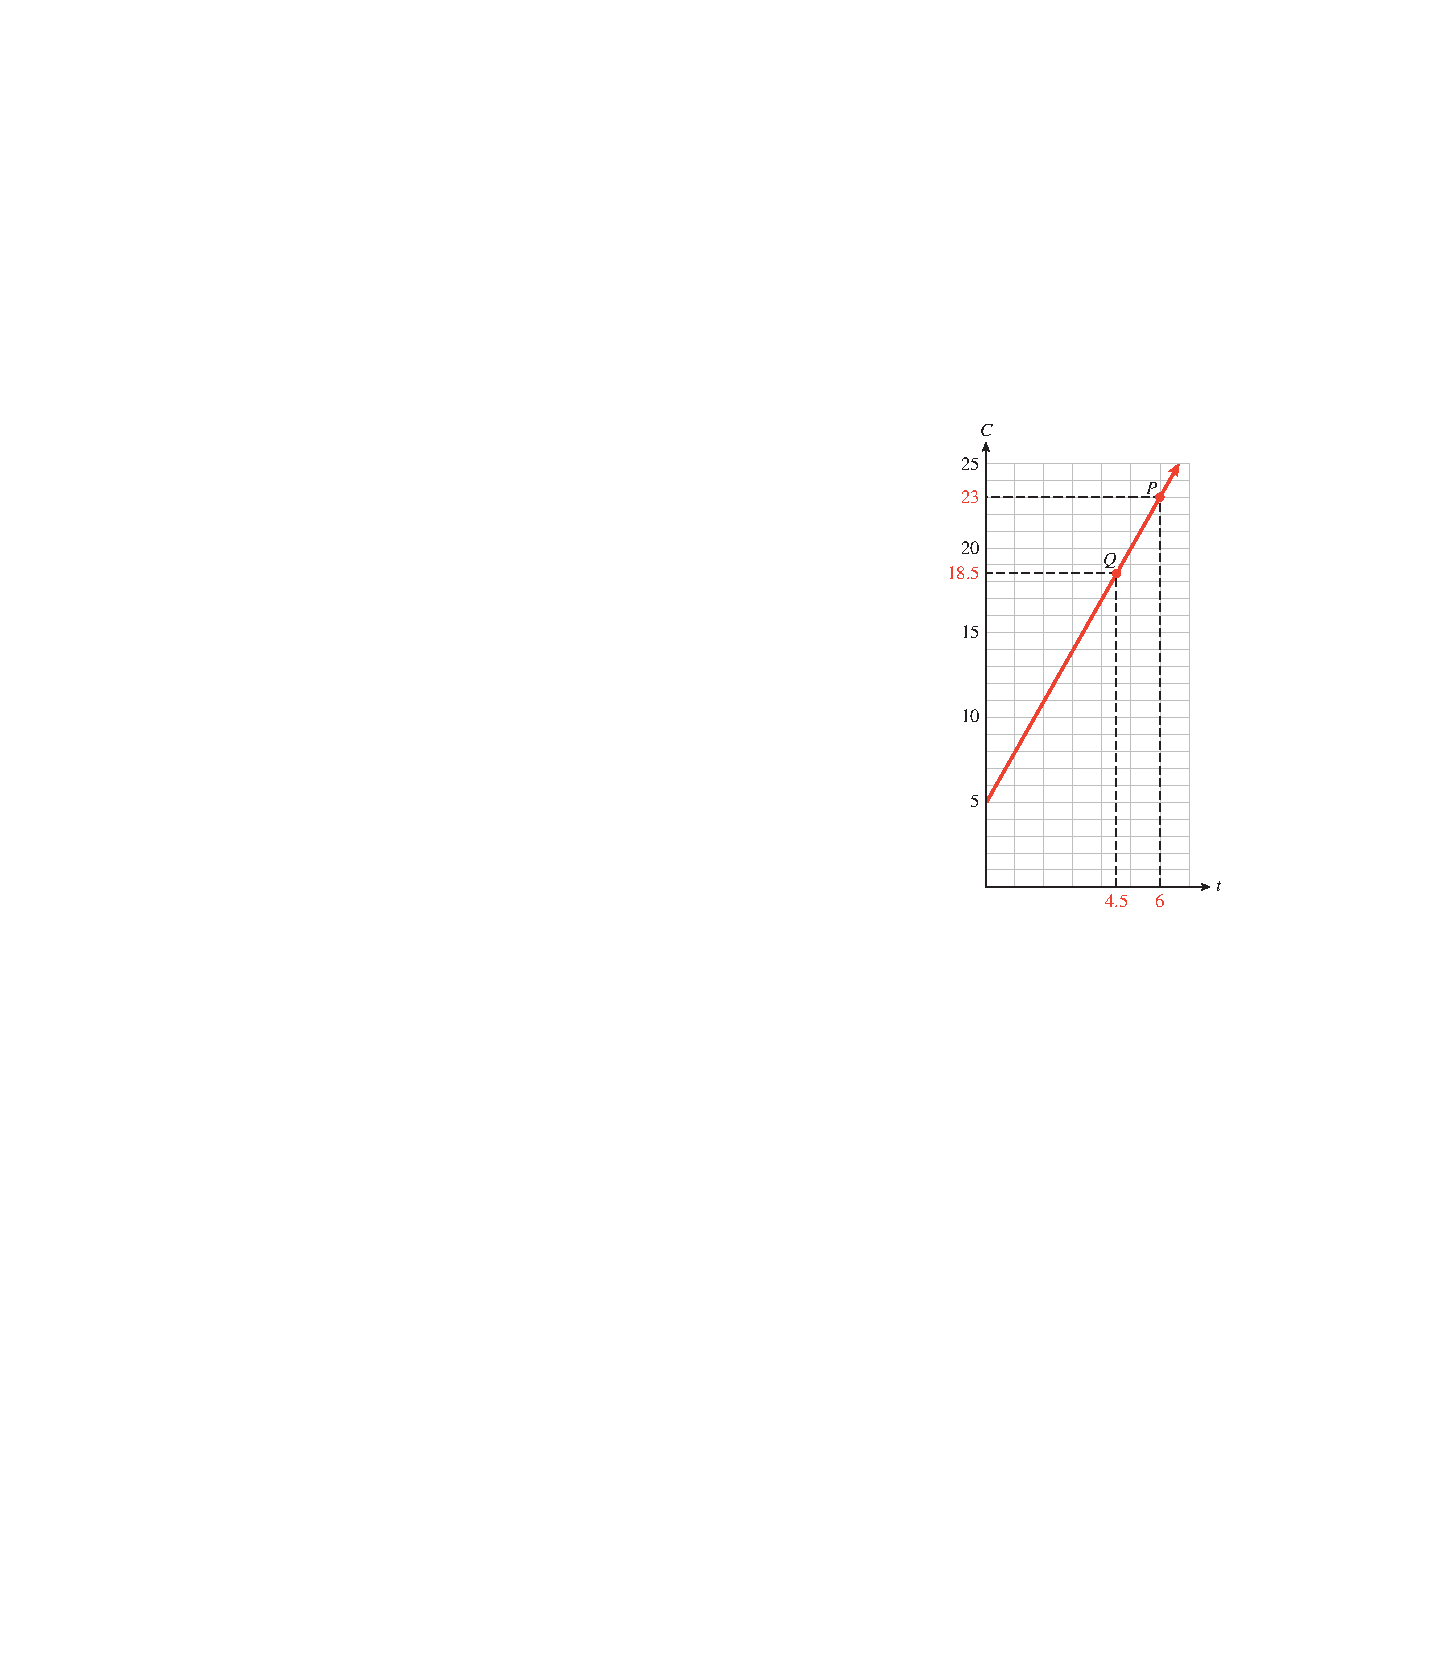
\includegraphics[width=0.50\textwidth,]{images/fig1-2.pdf}\end{figure}
\end{example}
\par
In \hyperref[example-6hrbike]{Example~\ref{example-6hrbike}}, notice the different algebraic techniques we used in parts (a) and (b).   In part (a), we were given a value of \(t\) and we \terminology{evaluated the expression}  \(5+3t\) to find \(C\).  In part (b) we were given a value of \(C\) and we \terminology{solved the equation} \(C=5+3t\) to find \(t.\)%
\begin{exercise}\label{exercise-Frank-plants}
 Frank plants a dozen corn seedlings, each 6 inches tall.  With plenty of water and sunlight they will grow approximately 2 inches per day.  Complete the table of values for the height, \(h\), of the seedlings after \(t\) days.%
\leavevmode%
\begin{figure}
\centering
\pushValignCaptionBottom[b]{minipage}{.50\textwidth}{%
\centering% horizontal alignment 
\begin{tabular}{AcAcAcAcAcAcA}\hrulethick
\(t\)&0&5&10&15&20\tabularnewline\hrulethin
\(h\)&&&&&\tabularnewline\hrulethin
\end{tabular}
}% end body 
{}% caption 
\pushValignCaptionBottom[b]{minipage}{.50\textwidth}{%
\centering% horizontal alignment 
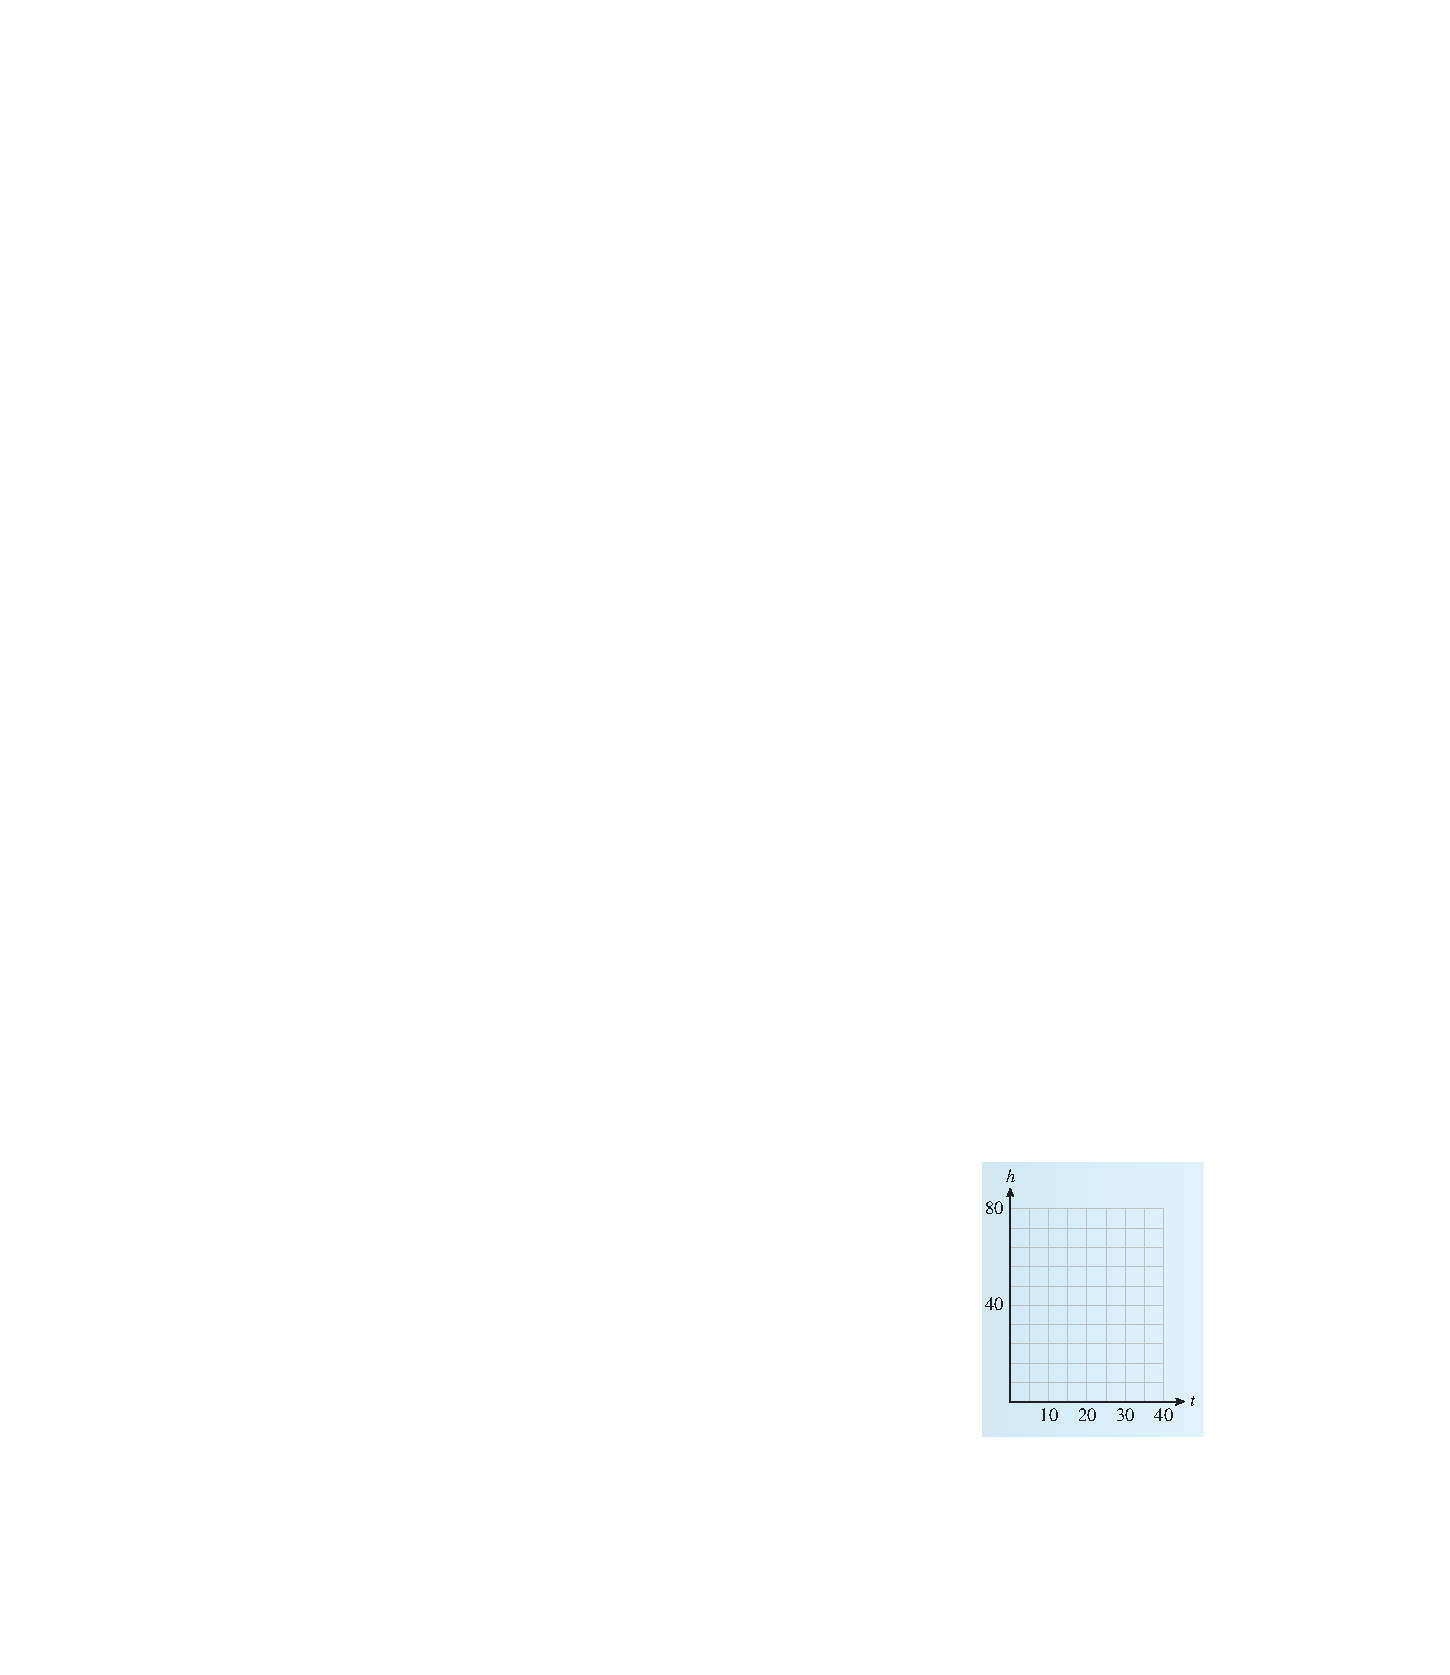
\includegraphics[width=\textwidth,]{images/fig-Example2.pdf}}% end body 
{}% caption 
\popValignCaptionBottom
\end{figure}
\leavevmode%
\begin{enumerate}[label=*\alph**]
\item\hypertarget{li-23}{}Write an equation for the height of the seedlings in terms of the number of days since they were planted.%
\item\hypertarget{li-24}{}Graph the equation.%
\end{enumerate}
\end{exercise}
\begin{exercise}\label{exercise-2}
 Use your equation from \hyperref[exercise-Frank-plants]{Exercise~\ref{exercise-Frank-plants}} to answer the questions.  Illustrate each answer on the graph. %
\leavevmode%
\begin{enumerate}[label=*\alph**]
\item\hypertarget{li-25}{} How tall is the corn after 3 weeks? %
\item\hypertarget{li-26}{} How long will it be before the corn is 6 feet tall? %
\end{enumerate}
\end{exercise}
\typeout{************************************************}
\typeout{Subsection 1.1.2 Choosing Scales for the Axes}
\typeout{************************************************}
\subsection[Choosing Scales for the Axes]{Choosing Scales for the Axes}\label{subsection-2}
To draw a useful graph, we must choose appropriate scales for the axes.  They must extend far enough to show the values of the variables, and the tick marks should be equally spaced.  Usually no more than 10 or 15 tick marks are needed.%
\begin{example}[]\label{example-home-price}
In 1990, the median home price in the US was \textdollar{}92,000.  The median price increased by about \textdollar{}4700 per year over the next decade.
        \leavevmode%
\begin{enumerate}[label=*\alph**]
\item\hypertarget{li-27}{} Make a table of values showing the median price of a house in 1990, 1994, 1998, and 2000.%
\item\hypertarget{li-28}{} Choose suitable scales for the axes and plot the values you found in part (a) on a graph. Use \(t\), the number of years since 1990, on the horizontal axis and the price of the house, \(P\), on the vertical axis.  Draw a curve through the points.%
\item\hypertarget{li-29}{} Write an equation that expresses \(P\) in terms of \(t\).%
\item\hypertarget{li-30}{} How much did the price of the house increase from 1990 to 1996?  Illustrate the increase on your graph.%
\end{enumerate}

    %
\par\medskip\noindent%
\textbf{Solution.}\quad \leavevmode%
\begin{enumerate}[label=*\alph**]
\item\hypertarget{li-31}{}In 1990 the median price was \textdollar{}92,000.  Four years later, in 1994, the price had increased by \(\alert{4}(4700)=18,800\) dollars, so
        \begin{equation*}P=92,000+\alert{4}(4700)=110,800\end{equation*}
        In 1998 the price had increased by \(\alert{8}(4700)=37,600\)  dollars, so
        \begin{equation*}P=92,000+\alert{8}(4700)-129,600\end{equation*}
        You can verify the price of the house in 2000 by a similar calculation.%
\leavevmode%
\begin{table}
\centering
\begin{tabular}{AcAcAcA}\hrulethick
Year%
&Price of House)%
&\((t,P)\)\tabularnewline\hrulethin
1990&92,000&\((0, 92,000)\)\tabularnewline\hrulethin
1994&110,800&\((4, 110,800)\)\tabularnewline\hrulethin
1998&129,600&\((8, 129,600)\)\tabularnewline\hrulethin
2000&139,000&\((10, 139,000)\)\tabularnewline\hrulethin
\end{tabular}
\end{table}
\item\hypertarget{li-32}{}Let \(t\) stand for the number of years since 1990, so that \(t=0\) in 1990, \(t=4\) in 1994, and so on.  To choose scales for the axes,
             look at the values in the table.  For this graph we scale the horizontal axis, or \(t\)-axis, in 1-year intervals and the vertical axis, or \(P\)-axis, for \textdollar{}90,000 to \textdollar{}140,000 in intervals of \textdollar{}5,000. The points in Figure 1. lie on a straight line.%
\item\hypertarget{li-33}{}Look back at the calculations in part (a).  The price of the house started at \textdollar{}92,000 in 1990 and increased by \(t \times 4700\) dollars after \(t\) years.  Thus,
            \begin{equation*}P=92,000+4700t\end{equation*}%
\item\hypertarget{li-34}{}Find the points on the graph corresponding to 1990 and 1996.  These points lie above \(t=0\) and \(t=6\) on the \(t\)-axis.  Now find the values on the \(P\)-axis corresponding to the two points.  The values are \(P=92,000\) in 1990 and \(P=120,200\) in 1996.  The increase in price is the difference of the two \(P\)-values.
            \begin{align*}
\text{increase in price}\amp=120,200-92,000
                \\
\amp=28,200
\end{align*}  
            The price of the home increased \textdollar{}28,200 between 1990 and 1996.  This increase is indicated by the arrows in \hyperref[fig-median-house]{Figure~\ref{fig-median-house}} [ref].%
\leavevmode%
\begin{figure}
\centering
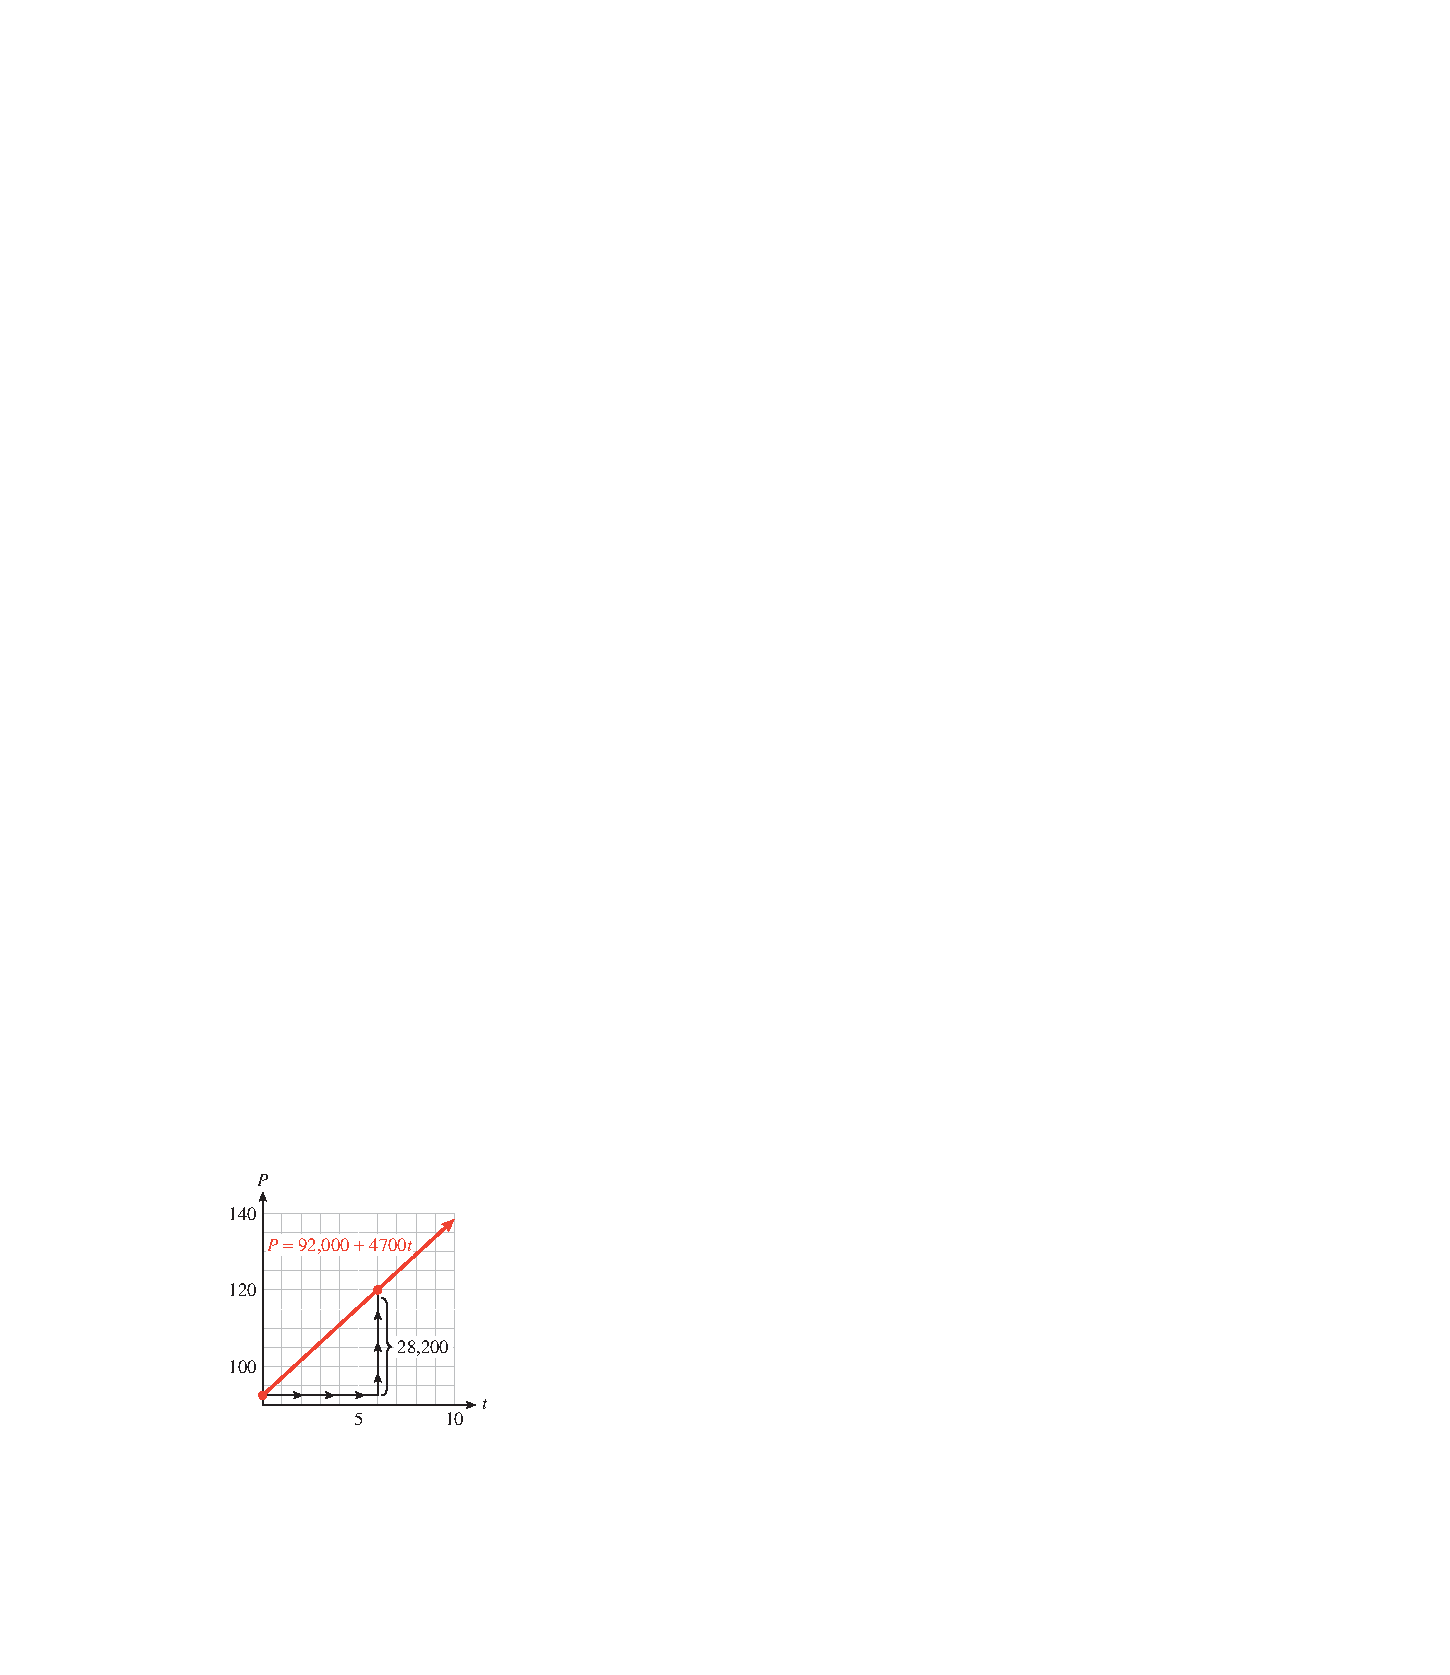
\includegraphics[width=0.50\textwidth,]{images/fig1-3.pdf}\caption{\label{fig-median-house}}
\end{figure}
\end{enumerate}
\end{example}
\par
The graphs in the preceding examples are \terminology{increasing graphs}.  As we move along the graph from left to right (in the direction of increasing \(t\) ), the second coordinate increases as well.  Try Exercise 3, which illustrates a \terminology{decreasing graph}.%
\begin{exercise}\label{exercise-Silver-Lake}
Silver Lake has been polluted by industrial waste products.  The concentration of toxic chemicals in the water is currently 285 parts per million (ppm).  Local environmental officials would like to reduce the concentration by 15 ppm each year%
\leavevmode%
\begin{enumerate}[label=*\alph**]
\item\hypertarget{li-35}{}Complete the table of values showing the desired concentration, \(C,\)~ of toxic chemicals \(t\) years from now.  For each \(t\)-value, calculate the corresponding value for \(C\).  Write your answers as ordered pairs.%
\leavevmode%
\begin{table}
\centering
\begin{tabular}{AcAcAcAcA}\hrulethick
\(t\)%
&\(C\)%
&&\((t,C)\)\tabularnewline\hrulethin
0&&\(C=285-150(\alert{0})\)&\((0, ~~~~ )\)\tabularnewline\hrulethin
5&&\(C=285-150(\alert{5})\)&\((5, ~~~~ )\)\tabularnewline\hrulethin
10&&\(C=285-150(\alert{10})\)&\((10, ~~~~ )\)\tabularnewline\hrulethin
15&&\(C=285-150(\alert{15})\)&\((15, ~~~~ )\)\tabularnewline\hrulethin
\end{tabular}
\end{table}
\item\hypertarget{li-36}{}To choose scales for the axes, notice that the value of \(C\) starts at 285 and decreases from there.  We'll scale the vertical axis up to 300, and use 10 tick marks at intervals of 30.  Graph the ordered pairs on the grid, and connect them with a straight line. Extend the graph until it reaches the horizontal axis, but no farther.  Points with negative \(C\)-coordinates have no meaning for the problem.%
\item\hypertarget{li-37}{}Write an equation for the concentration, \(C\), of toxic chemicals \(t\) years from now.  (Hint:  The concentration is initially 8 ppm, and we subtract 15 ppm for each year that passes, or \(15 \times t\).)%
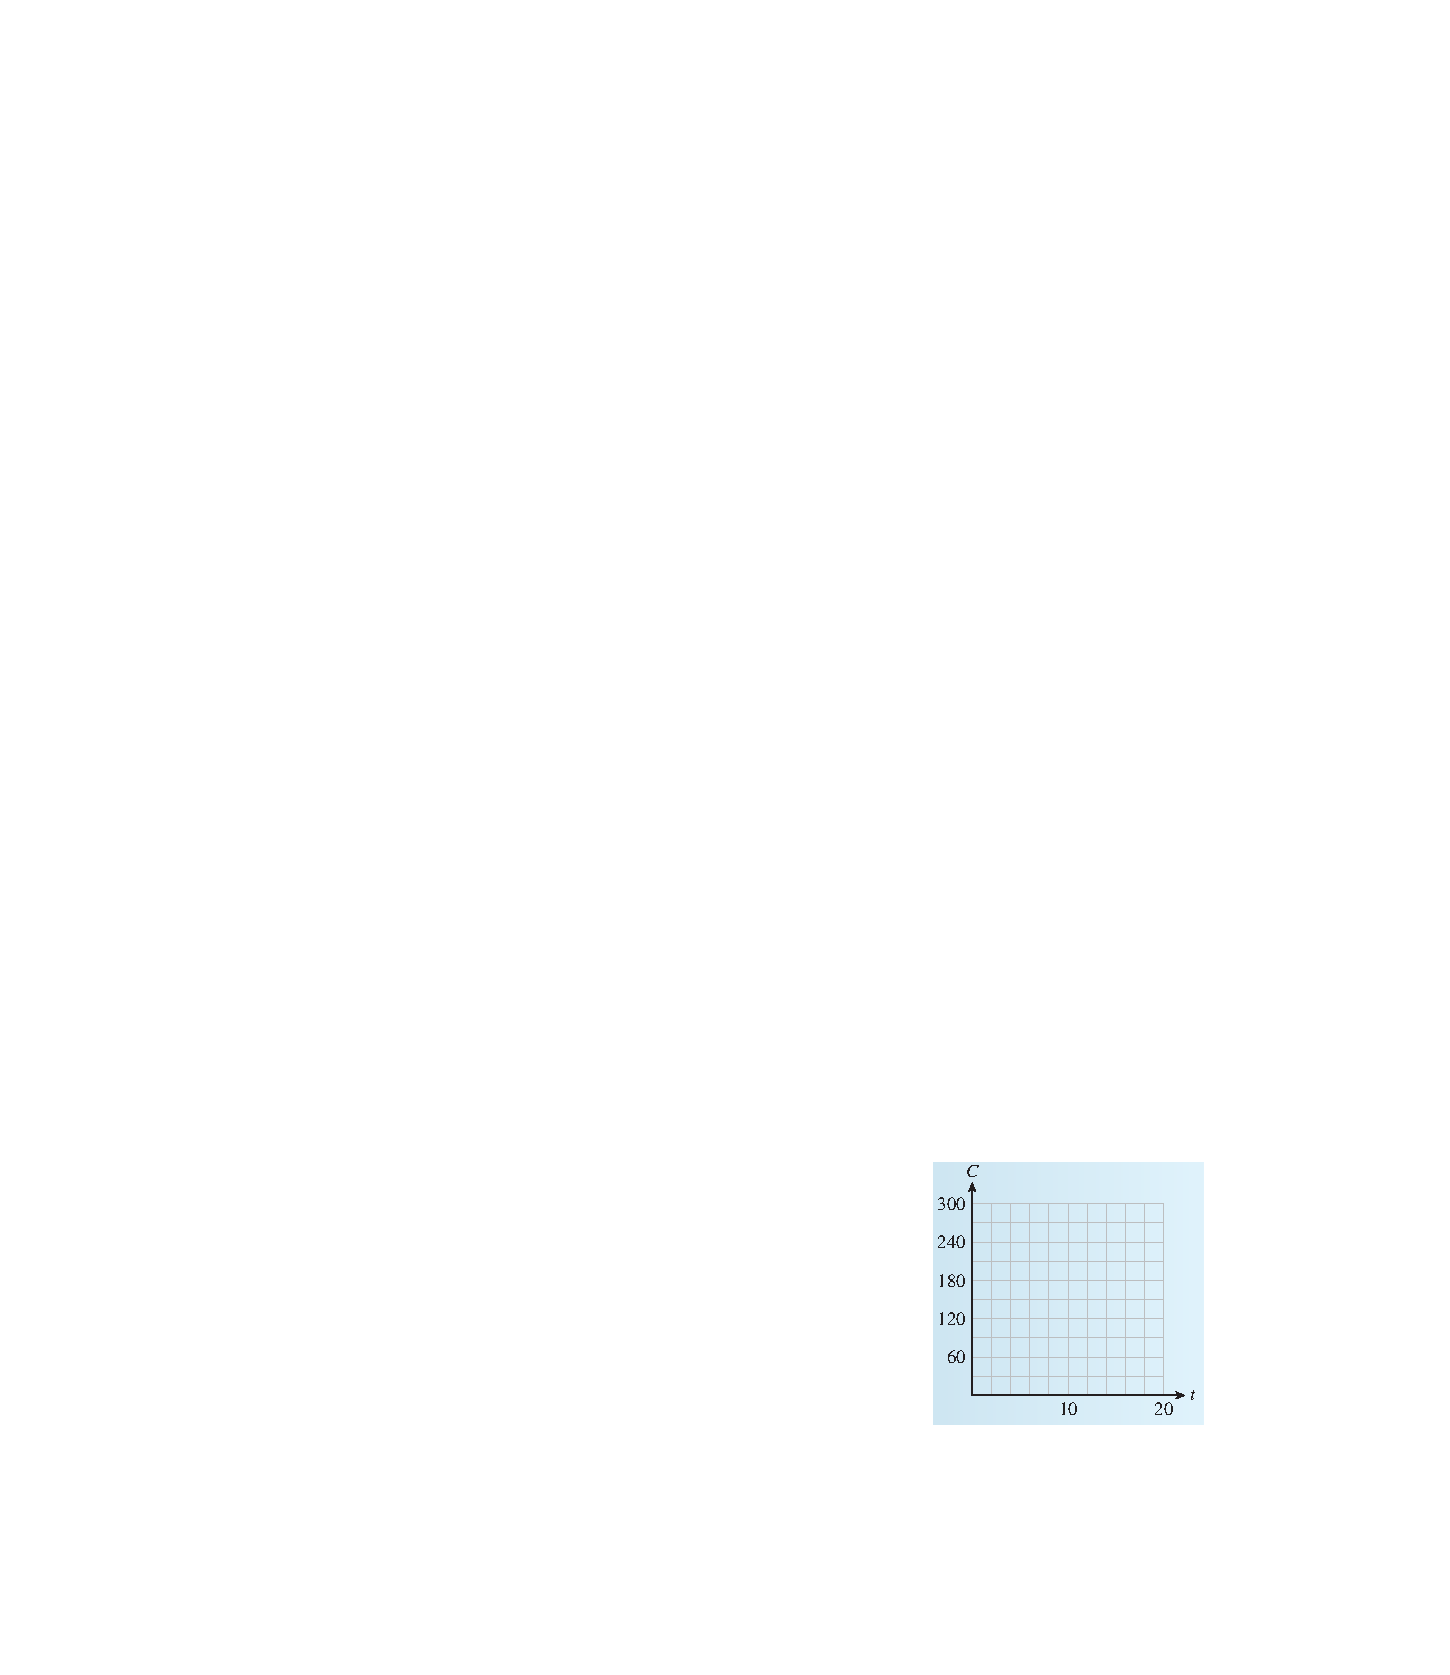
\includegraphics[width=0.50\textwidth,]{images/fig-Exercise3.pdf}\end{enumerate}
\end{exercise}
\begin{remark}[
\includegraphics[width=0.8\textwidth,]{images/icon-GC.pdf}Graphing an Equation]\label{remark-1}
We can use a graphing calculator to graph an equation. On most calculators, we follow three steps.%
\par
To Graph an Equation:%
\leavevmode%
\begin{enumerate}
\item\hypertarget{li-38}{}Press \lstinline?Y=? and enter the equation you wish to graph.%
\item\hypertarget{li-39}{}Press \lstinline?WINDOW? and select a suitable graphing window.%
\item\hypertarget{li-40}{}Press \lstinline?GRAPH?%
\end{enumerate}
\end{remark}
\begin{example}[
\includegraphics[width=0.8\textwidth,]{images/icon-GC.pdf}Using a Graphing Calculator]\label{graphing-calculator}
In \hyperref[example-home-price]{Example~\ref{example-home-price}}, we found the equation \(P = 92,000 + 4700t\) for the median price of a house \(t\) years after 1990. Graph this equation on a calculator.%
\par\medskip\noindent%
\textbf{Solution.}\quad 
            To begin, we press \lstinline?Y=? and enter
        %
\par

             \begin{equation*}Y1 = 92,000 + 4700X\end{equation*}
        %
\par
For this graph, we’ll use the grid in \hyperref[example-home-price]{Example~\ref{example-home-price}} for our window settings, so we press \lstinline?WINDOW? and enter
        %
\leavevmode%
\begin{table}
\centering
\begin{tabular}{lll}
Xmin\(=0\)&&Xmax\(=10\)\tabularnewline[0pt]
Ymin\(=90,000\)&&Ymax\(=140,000\)
\end{tabular}
\end{table}
\par

        Finally, we press \lstinline?GRAPH?. The calculator’s graph is shown in \hyperref[fig-GC-house-price]{Figure~\ref{fig-GC-house-price}}.%
\leavevmode%
\begin{figure}
\centering
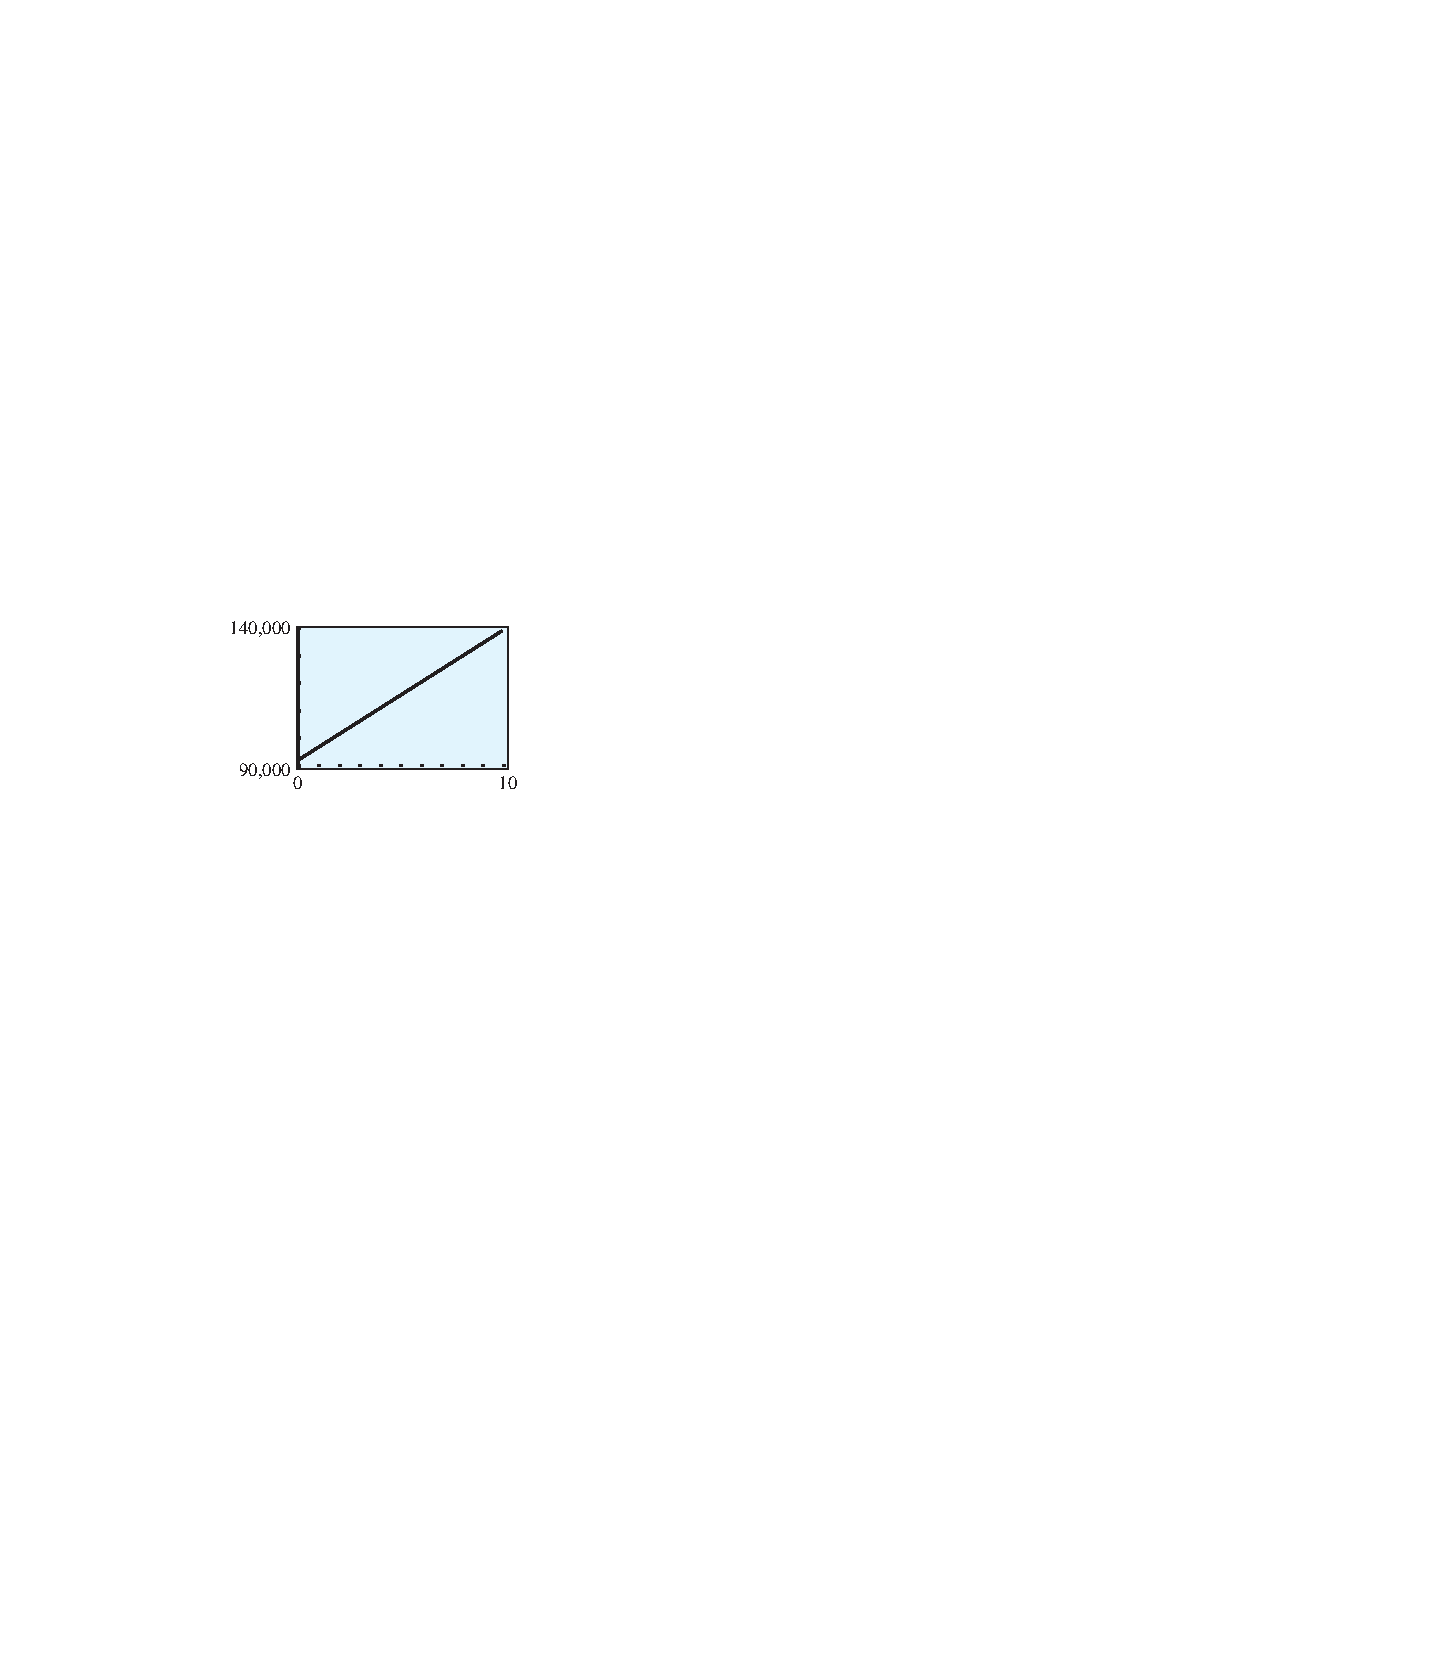
\includegraphics[width=0.50\textwidth,]{images/fig-GC-house-price.pdf}\caption{\label{fig-GC-house-price}}
\end{figure}
\end{example}
\begin{exercise}\label{exercise-gc}
\leavevmode%
\begin{enumerate}[label=*\alph**]
\item\hypertarget{li-41}{}Solve the equation \(2y − 1575 = 45x\) for \(y\) in terms of \(x\).%
\item\hypertarget{li-42}{}Graph the equation on a graphing calculator. Use the window
        \leavevmode%
\begin{table}
\centering
\begin{tabular}{lllll}
Xmin\(=-50\)&&Xmax\(=50\)&&Xscl\(=5\)\tabularnewline[0pt]
Ymin\(=-500\)&&Ymax\(=1000\)&&Yscl\(=100\)
\end{tabular}
\end{table}
%
\item\hypertarget{li-43}{}Sketch the graph on paper. Use the window settings to choose appropriate scales for the axes.%
\end{enumerate}
\end{exercise}
\typeout{************************************************}
\typeout{Subsection 1.1.3 Linear Equations}
\typeout{************************************************}
\subsection[Linear Equations]{Linear Equations}\label{subsection-3}
All the models in these examples have equations with a similar form:  \begin{equation*}y=\text{(starting value)}+\text{(rate of change)}\cdot x\end{equation*}
(We'll talk more about rate of change in Section 1.4.)  Their graphs were all portions of straight lines.  For this reason such equations are called  \terminology{linear equations}.  The order of the terms in the equation does not matter.  For example, the equation in Example 1, \begin{equation*}C=5+3t\end{equation*} can be written equivalently as \begin{equation*}-3t+C=5\end{equation*} and the equation in Example 3, \begin{equation*}P=92,000+4700t\end{equation*} can be written as \begin{equation*}-4700+P=92,000\end{equation*} 
This form of a linear equation, \begin{equation*}Ax+By=C\end{equation*} is called the \terminology{general form}.%
\typeout{************************************************}
\typeout{Paragraphs  General Form for a Linear Equation}
\typeout{************************************************}
\paragraph[General Form for a Linear Equation]{General Form for a Linear Equation}\label{paragraphs-2}
The graph of any equation \begin{equation*}Ax+By=C\end{equation*} where \(A\) and \(B\) are not both equal to zero, is a straight line.%
\begin{example}[]\label{example-advertising}
The manager at Albert's Appliances has \textdollar{}3000 to spend on advertising for the next fiscal quarter.  A 30-second spot on television costs \textdollar{}150 per broadcast, and a 30-second radio ad costs \textdollar{}50.%
\leavevmode%
\begin{enumerate}[label=*\alph**]
\item\hypertarget{li-44}{}The manager decides to buy \(x\) television ads and \(y\) radio ads.  Write an equation relating \(x\) and \(y\).%
\item\hypertarget{li-45}{}Make a table of values showing several choices for \(x\) and \(y\).%
\item\hypertarget{li-46}{}Plot the points from your table, and graph the equation.%
\end{enumerate}
\par\medskip\noindent%
\textbf{Solution.}\quad \leavevmode%
\begin{enumerate}[label=*\alph**]
\item\hypertarget{li-47}{}Each television ad costs \textdollar{}150, so ads will cost \textdollar{}150.  Similarly, radio ads will cost \textdollar{}50.  The manager has \textdollar{}3000 to spend, so the sum of the costs must be \textdollar{}3000.  Thus, \begin{equation*}150x+50y=3000\end{equation*}%
\item\hypertarget{li-48}{}Choose some values of \(x\), and solve the equation for the corresponding value of \(y\)  For example, if \(x=\alert{10}\) then
               \begin{align*}
150(10)+50y\amp=300\\
1500+50y\amp=3000\\
50y\amp=1500\\
y\amp=30
\end{align*}
                If the manager buys 10 television ads, she can also buy 30 radio ads.  You can verify the other entries in the table.%
\leavevmode%
\begin{table}
\centering
\begin{tabular}{AcAcAcAcAcA}\hrulethick
\(x\)&8&10&12&14\tabularnewline\hrulethin
\(y\)&&&&\tabularnewline\hrulethin
\end{tabular}
\end{table}
\item\hypertarget{li-49}{}Plot the points from the table.  All the solutions lie on a straight line, as shown in \hyperref[fig-example-advertising]{Figure~\ref{fig-example-advertising}}
.
        \leavevmode%
\begin{figure}
\centering
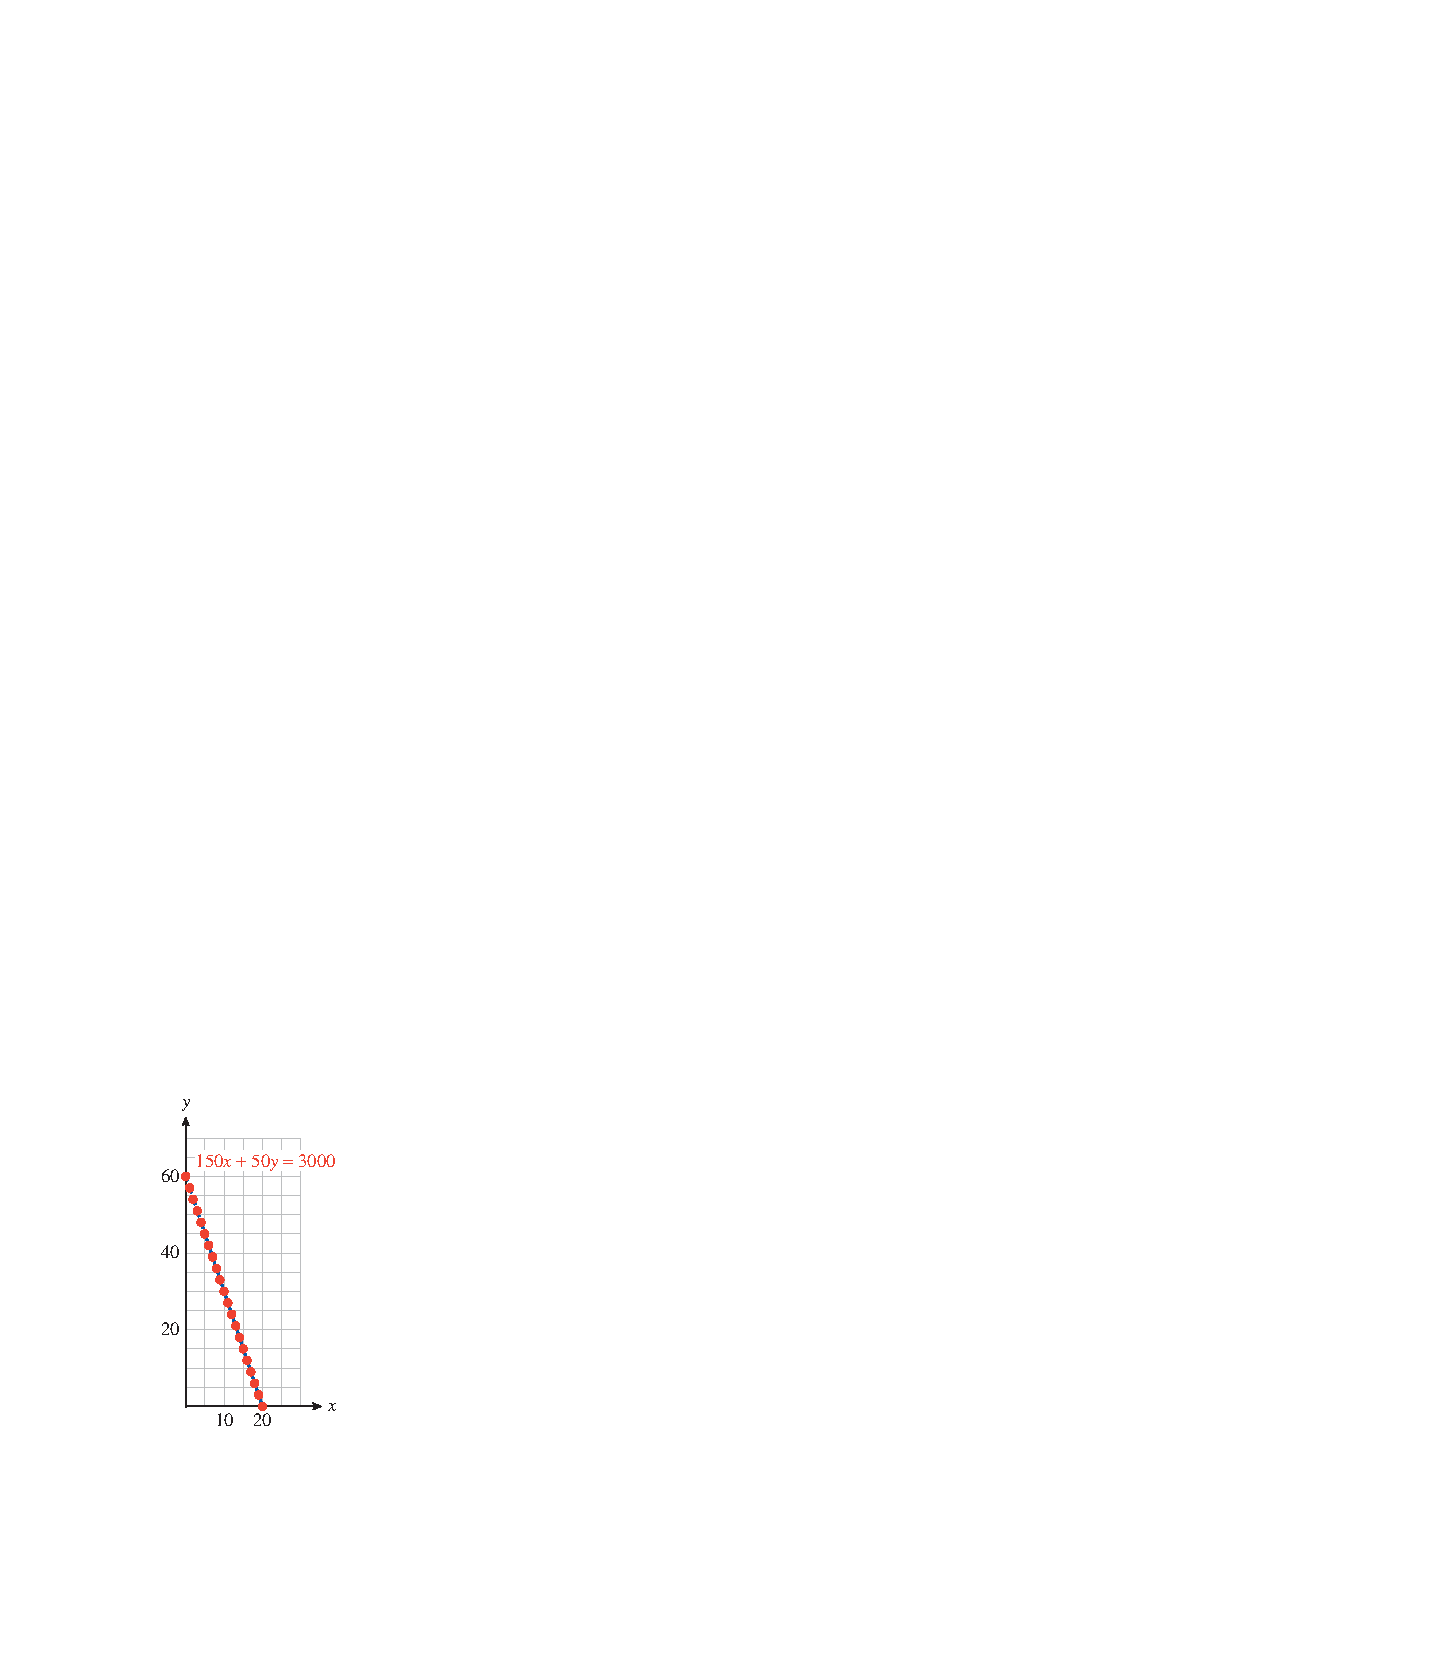
\includegraphics[width=0.50\textwidth,]{images/fig-example-advertising.pdf}\caption{\label{fig-example-advertising}}
\end{figure}
%
\end{enumerate}
\end{example}
\begin{exercise}\label{exercise-crops}
In central Nebraska, each acre of corn requires 25 acre-inches of water per year, and each acre of winter wheat requires 18 acre-inches of water.             (An acre-inch is the amount of water needed to cover one acre of land to a depth of one inch.)  A farmer can count on 9000 acre-inches of water for the coming year.  (Source:  Institute of Agriculture and Natural Resources, University of Nebraska)
    \leavevmode%
\begin{enumerate}[label=*\alph**]
\item\hypertarget{li-50}{}Write an equation relating the number of acres of corn, \(x\), and the number of acres of wheat, \(y\), that the farmer can plant.%
\item\hypertarget{li-51}{}Complete the table.%
\leavevmode%
\begin{table}
\centering
\begin{tabular}{AcAcAcAcAcA}\hrulethick
\(x\)&50&100&150&200\tabularnewline\hrulethin
\(y\)&&&&\tabularnewline\hrulethin
\end{tabular}
\end{table}
\end{enumerate}
%
\end{exercise}
\typeout{************************************************}
\typeout{Subsection 1.1.4 Intercepts}
\typeout{************************************************}
\subsection[Intercepts]{Intercepts}\label{subsection-4}
\leavevmode%
\begin{figure}
\centering
\pushValignCaptionBottom[b]{minipage}{.50\textwidth}{%
\centering% horizontal alignment 
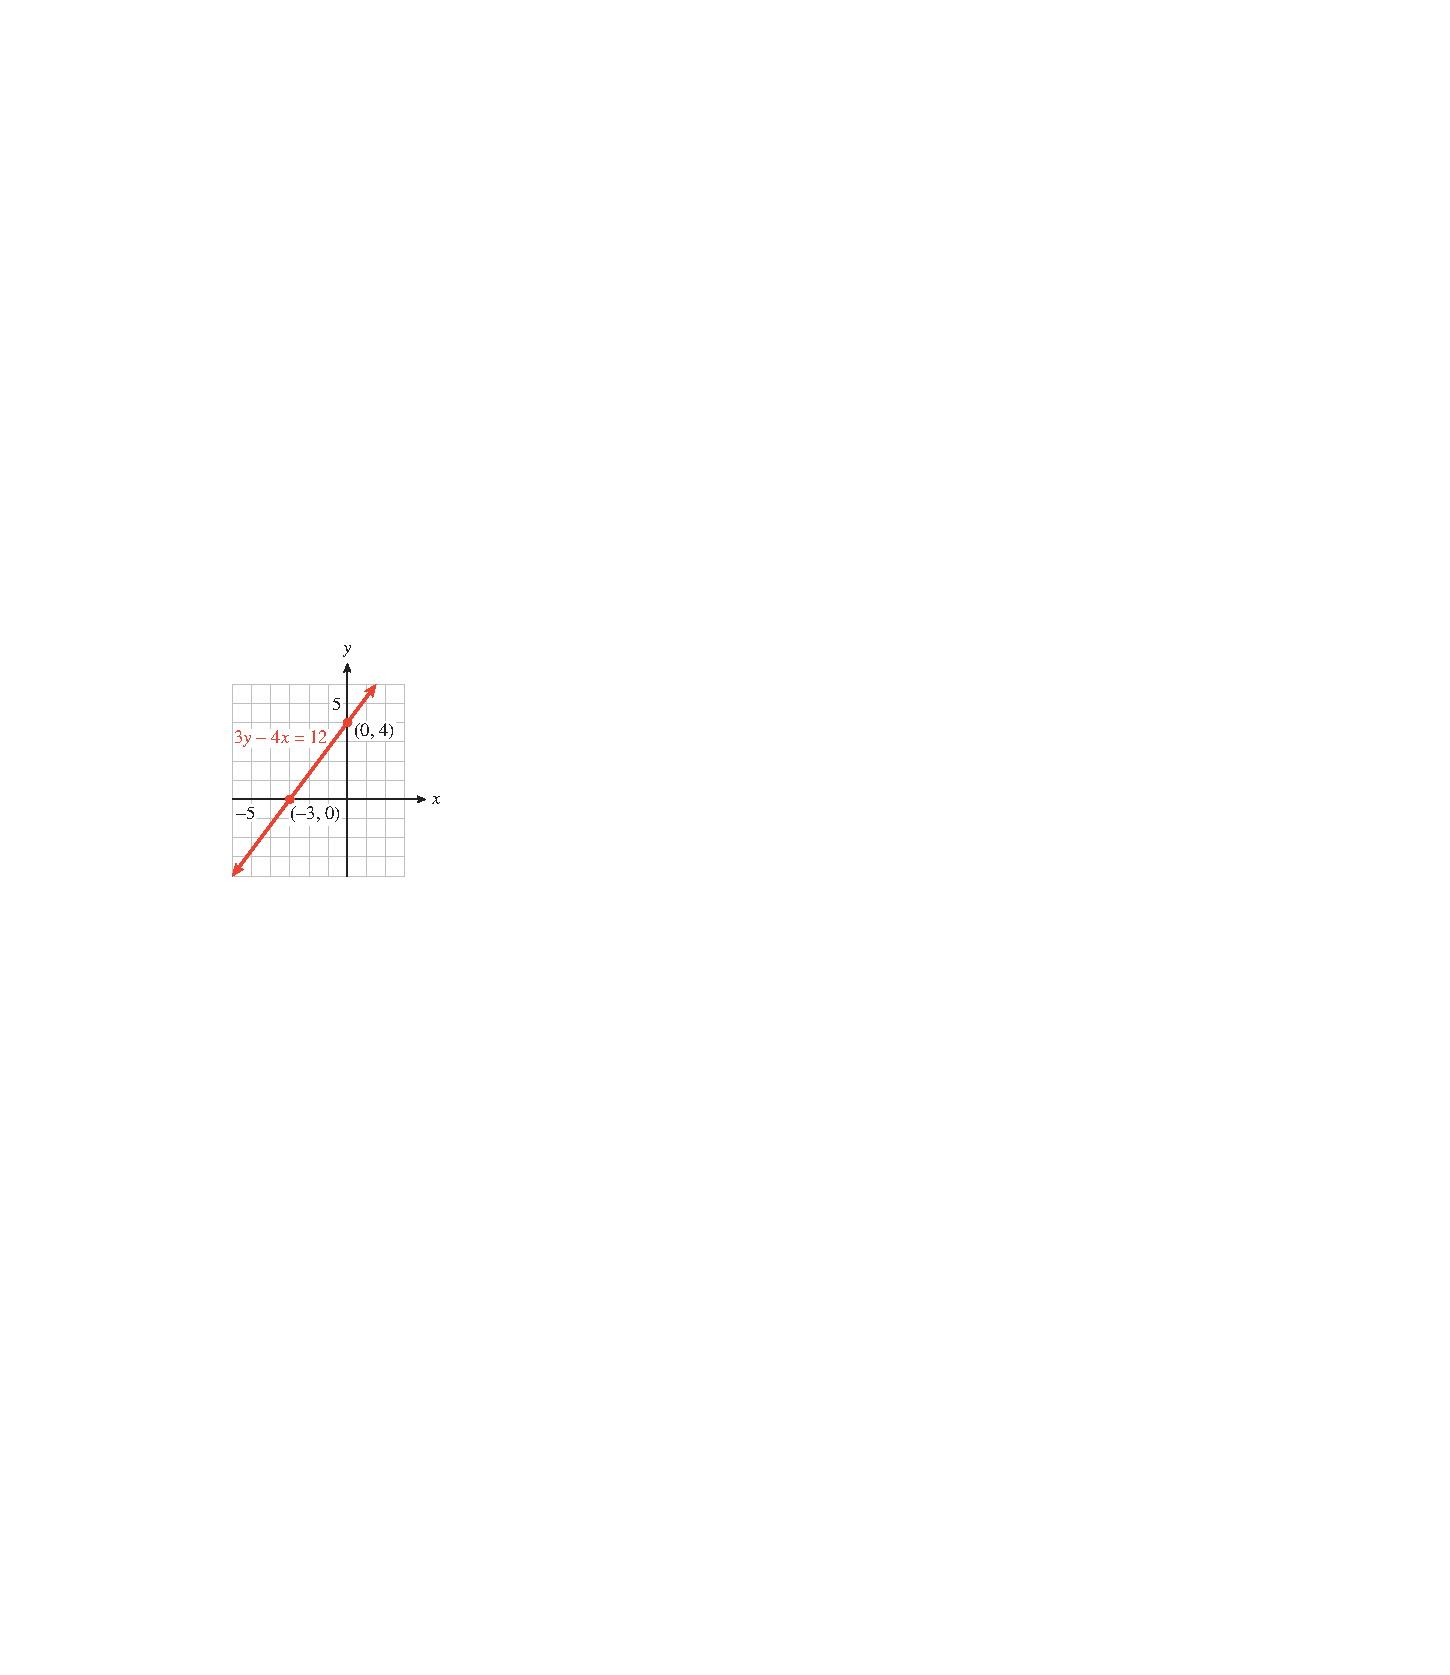
\includegraphics[width=\textwidth,]{images/fig-intercepts.pdf}}% end body 
{\captionof{figure}{\label{fig-intercepts}}
}% caption 
\pushValignCaptionBottom[b]{minipage}{.50\textwidth}{%
\parbox{\textwidth}{%
% horizontal alignment 
Consider the graph of the equation \begin{equation*}3x-4y=12\end{equation*} shown in \hyperref[fig-intercepts]{Figure~\ref{fig-intercepts}}. The points where the graph crosses the axes are called the \terminology{intercepts} of the graph. The coordinates of these points are easy to find.  The \(y\)-coordinate of the \(x\)-intercept is zero, so we set \(y=\alert{0}\) in the equation to get \begin{align*}
3(\alert{0})-4x\amp=12\\
x=-3
\end{align*} 
        }%
}% end body 
{}% caption 
\popValignCaptionBottom
\end{figure}
The \(x\)-intercept is the point\((-3,0)\). Also, the \(x\)-coordinate of the \(y\)-intercept is zero, so we set \(x=\alert{0}\) in the equation to get \begin{gather*}
3y-4(\alert{0})=12\\
y=4
\end{gather*}  The \(y\)-intercept is \((0,4)\).%
\typeout{************************************************}
\typeout{Paragraphs  Intercepts of a Graph}
\typeout{************************************************}
\paragraph[Intercepts of a Graph]{Intercepts of a Graph}\label{paragraphs-3}
The points where a graph crosses the axes are called the \terminology{intercepts of the graph}.%
\leavevmode%
\begin{enumerate}
\item\hypertarget{li-52}{}To find the \(y\)-intercept, set \(x=0\) and solve for \(y\).%
\item\hypertarget{li-53}{}To find the \(x\)-intercept, set \(y=0\) and solve for \(x\)%
\end{enumerate}
\par

      The intercepts of a graph tell us something about the situation it models.  
    %
\begin{example}[]\label{example-intercepts}
\leavevmode%
\begin{enumerate}[label=*\alph**]
\item\hypertarget{li-54}{}
        Find the intercepts of the graph in \hyperref[exercise-Silver-Lake]{Exercise~\ref{exercise-Silver-Lake}}, about the pollution in Silver Lake.
    \item\hypertarget{li-55}{}What do the intercepts tell us about the problem?
    \end{enumerate}
\par\medskip\noindent%
\textbf{Solution.}\quad \leavevmode%
\begin{enumerate}[label=*\alph**]
\item\hypertarget{li-56}{}An equation for the concentration of toxic chemicals is \begin{equation*}C=285-15t\end{equation*} To find the \(C\)-intercept, set \(t\) equal to zero. 

            \begin{equation*}C=285-15(0)=285\end{equation*}
            The \(C\)-intercept is the point \((0, 285)\), or simply 285.  To find the \(t\)-intercept, set \(C\) equal to zero and solve for \(t\).
            
                \begin{align*}
                \alert{0}\&=285-15t \&\&\text{Add }15t \text{ to both sides.}\textbackslash{}\textbackslash{}
                15t\&=285  \&\&\text{Divide both sides by 15.}\textbackslash{}\textbackslash{}
                t\&=19   \&\& 
                \end{align*}
            %


        The \(t\)-intercept is the point \((19,0)\), or simply \(19\).%
\item\hypertarget{li-57}{}The \(C\)-intercept represents the concentration of toxic chemicals in Silver Lake now:  When  \(t=0\), \(C=285\),  so the concentration is currently \(285\) ppm.  The \(t\)-intercept represents the number of years it will take for the concentration of toxic chemicals to drop to zero:  When \(C=0\), \(t=19\),  so it will take \(19\) years for the pollution to be eliminated entirely.%
\end{enumerate}
\end{example}
\begin{exercise}\label{exercise-6}
\leavevmode%
\begin{enumerate}[label=*\alph**]
\item\hypertarget{li-58}{}Find the intercepts of the graph in \hyperref[example-advertising]{Example~\ref{example-advertising}}, about the advertising budget for Albert’s Appliances: \(150x + 50y = 3000\).%
\item\hypertarget{li-59}{}What do the intercepts tell us about the problem?%
\end{enumerate}
\end{exercise}
\typeout{************************************************}
\typeout{Subsection 1.1.5 Intercept Method for Graphing Lines}
\typeout{************************************************}
\subsection[Intercept Method for Graphing Lines]{Intercept Method for Graphing Lines}\label{subsection-5}
Because we really only need two points to graph a linear equation, we might as well find the intercepts first and use them to draw the graph. The values of the intercepts will also help us choose suitable scales for the axes. It is always a good idea to find a third point as a check.
    %
\begin{example}[]\label{intercepts}
\leavevmode%
\begin{enumerate}[label=*\alph**]
\item\hypertarget{li-60}{}Find the \(x\)- and \(y\)-intercepts of the graph of \(150x − 180y = 9000\).%
\item\hypertarget{li-61}{}Use the intercepts to graph the equation. Find a third point as a check.%
\end{enumerate}
\par\medskip\noindent%
\textbf{Solution.}\quad \leavevmode%
\begin{enumerate}[label=*\alph**]
\item\hypertarget{li-62}{}To find the \(x\)-intercept, set \(y = \alert{0}\).
            %
\par

                \begin{align*}
                150x-18(\alert{0})\&=9000 \&\&\text{Simpify.}\textbackslash{}\textbackslash{}
                150x\&=9000  \&\&\text{Divide both sides by 150.}\textbackslash{}\textbackslash{}
                x\&=60   \&\& 
                \end{align*}
            %
\par
The \(x\)-intercept is the point \((60, 0)\). To find the \(y\)-intercept, set \(x = \alert{0}\).%
\par

                \begin{align*}
                150(\alert{0})-18y\&=9000 \&\&\text{Simpify.}\textbackslash{}\textbackslash{}
                -180y\&=9000  \&\&\text{Divide both sides by } -180\text{.}\textbackslash{}\textbackslash{}
                y\&=-50   \&\& 
                \end{align*}
            %
\par
The \(y\)-intercept is the point \((0, −50)\).%
\item\hypertarget{li-63}{}Scale both axes in intervals of 10 and then plot the two intercepts, \((60, 0)\) and \((0, −50)\). Draw the line through them, as shown in \hyperref[fig-example-graph-intercepts]{Figure~\ref{fig-example-graph-intercepts}}. Now find another point and check that it lies on this line. We choose \(x = \alert{20}\) and solve for \(y\).
            \begin{gather*}
150(\alert{20}) −180y = 9000\\
3000 −180y = 9000\\
−180y = 6000\\
y =−33.\overline{3}
\end{gather*}

            Plot the point \((20, −33\frac{1}{3})\). Because this point lies on the line, we can be reasonably confident that our graph is correct. 
            \leavevmode%
\begin{figure}
\centering
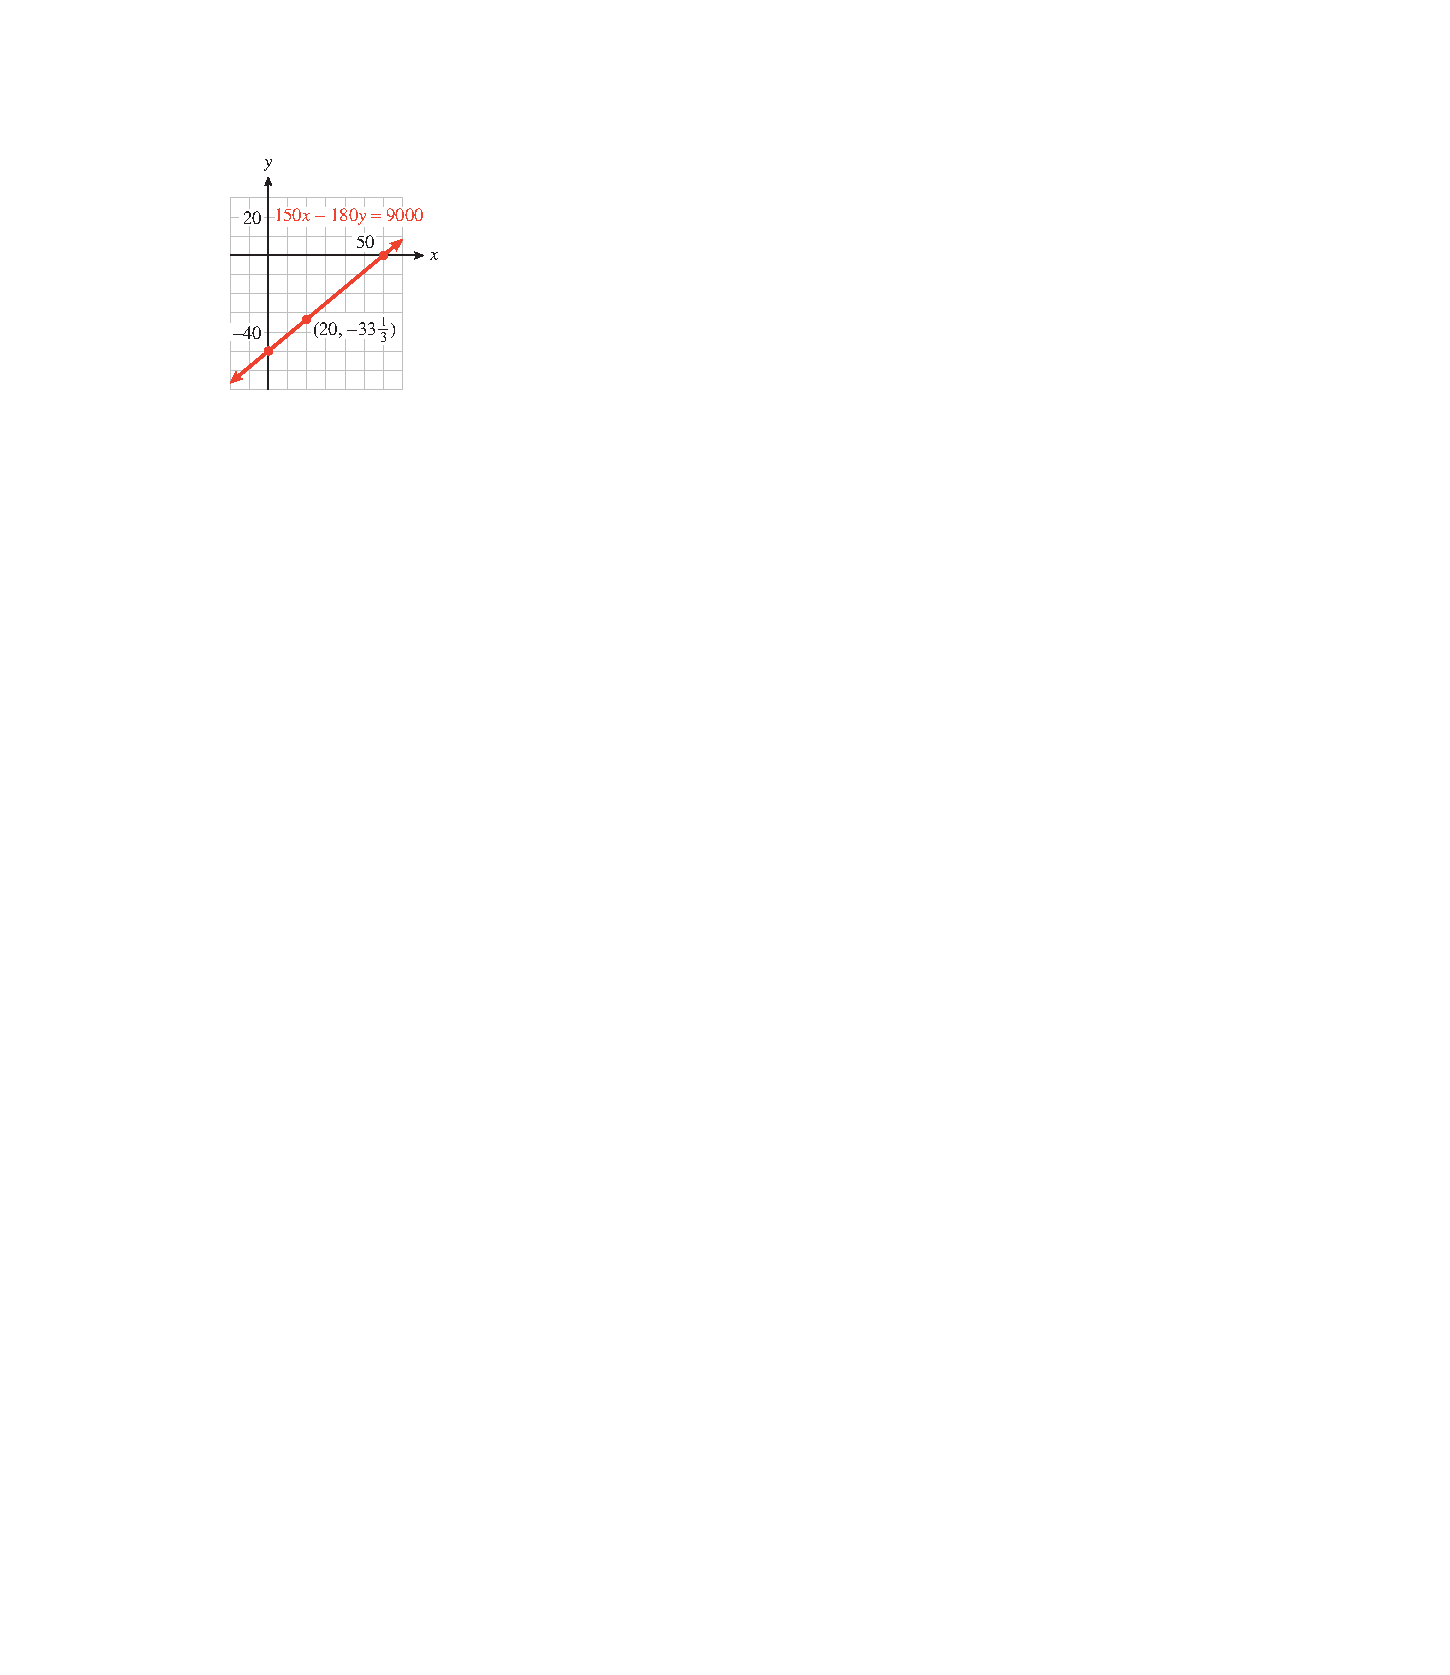
\includegraphics[width=0.50\textwidth,]{images/fig-example-graph-intercepts.pdf}\caption{\label{fig-example-graph-intercepts}}
\end{figure}

            %
\end{enumerate}
\end{example}
\begin{remark}[
\includegraphics[width=0.8\textwidth,]{images/icon-GC.pdf}Choosing a Graphing Window]\label{remark-2}
Knowing the intercepts can also help us choose a suitable window on a graphing calculator. We would like the window to be large enough to show the intercepts. For the graph in \hyperref[fig-example-graph-intercepts]{Figure~\ref{fig-example-graph-intercepts}}, we can enter the equation \begin{equation*}Y = (9000 −150X)/ −180\end{equation*}
    in the window
        \leavevmode%
\begin{table}
\centering
\begin{tabular}{lll}
Xmin\(=-20\)&&Xmax\(=70\)\tabularnewline[0pt]
Ymin\(=-70\)&&Ymax\(=30\)
\end{tabular}
\end{table}

    %
\end{remark}
\typeout{************************************************}
\typeout{Paragraphs  To Graph a Line Using the Intercept Method:}
\typeout{************************************************}
\paragraph[To Graph a Line Using the Intercept Method:]{To Graph a Line Using the Intercept Method:}\label{paragraphs-4}
\leavevmode%
\begin{enumerate}[label=*\arabic**]
\item\hypertarget{li-64}{}Find the intercepts of the line.%
\begin{enumerate}[label=++\alph*]
\item\hypertarget{li-65}{}To find the \(x\)-intercept, set \(y=0\) and solve for \(x\).%
\item\hypertarget{li-66}{}To find the \(y\)-intercept, set \(x = 0\) and solve for \(y\).%
\end{enumerate}
\item\hypertarget{li-67}{}Plot the intercepts.%
\item\hypertarget{li-68}{}Choose a value for \(x\) and find a third point on the line.%
\item\hypertarget{li-69}{}Draw a line through the points.%
\end{enumerate}
\begin{exercise}\label{exercise-intercepts}
\leavevmode%
\begin{enumerate}[label=*\alph**]
\item\hypertarget{li-70}{}In \hyperref[exercise-crops]{Exercise~\ref{exercise-crops}}, you wrote an equation about crops in Nebraska. Find the intercepts of the graph.%
\item\hypertarget{li-71}{}Use the intercepts to help you choose appropriate scales for the axes, and then graph the equation.%
\item\hypertarget{li-72}{}What do the intercepts tell us about the problem?%
\end{enumerate}
\end{exercise}
\par
The examples in this section model simple linear relationships between two variables.
Such relationships, in which the value of one variable is determined by the value of the
other, are called \terminology{functions}. We will study various kinds of functions throughout the course.%
\typeout{************************************************}
\typeout{Section 1.2 Functions}
\typeout{************************************************}
\section[Functions]{Functions}\label{functions}
\typeout{************************************************}
\typeout{Subsection 1.2.1 Definition of Function}
\typeout{************************************************}
\subsection[Definition of Function]{Definition of Function}\label{subsection-6}

    We often want to predict values of one variable from the values of a related variable. For example, when a physician prescribes a drug in a certain dosage, she needs to know how long the dose will remain in the bloodstream. A sales manager needs to know how the price of his product will affect its sales. A \terminology{function} is a special type of relationship between variables that allows us to make such predictions.%
\par

    Suppose it costs \textdollar{}800 for flying lessons, plus \textdollar{}30 per hour to rent a plane. If we let \(C\) represent the total cost for t hours of flying lessons, then
    \begin{equation*}C=800+305t ~~~~ (t\ge 0)\end{equation*}
    Thus, for example
%
\leavevmode%
\begin{table}
\centering
\begin{tabular}{rll}
when&\(t=\alert{0}\),&\(C=800+30(\alert{0})=800\)\tabularnewline[0pt]
when&\(t=\alert{4}\),&\(C=800+30(\alert{4})=920\)\tabularnewline[0pt]
when&\(t=\alert{10}\),&\(C=800+30(\alert{10})=1100\)
\end{tabular}
\end{table}
\par

    The variable \(t\) is called the \terminology{input} or \terminology{independent} variable, and \(C\) is the \terminology{output} or \terminology{dependent} variable, because its values are determined by the value of \(t\). We can display the relationship between two variables by a table or by ordered pairs. The input variable is the first component of the ordered pair, and the output variable is the second component.
%
\leavevmode%
\begin{table}
\centering
\begin{tabular}{AcAcAcA}\hrulethick
\(t\)&\(C\)&\((t,C)\)\tabularnewline\hrulethin
\(0\)&\(800\)&\((0, 800)\)\tabularnewline\hrulethin
\(4\)&\(920\)&\((4, 920)\)\tabularnewline\hrulethin
\(10\)&\(1100\)&\((10,1100)\)\tabularnewline\hrulethin
\end{tabular}
\end{table}
\par

    For this relationship, we can find the value \(C\) of associated with any given value of \(t\). All we have to do is substitute the value of \(t\) into the equation and solve for \(C\). The result has no ambiguity: Only one value for \(C\) corresponds to each value of \(t\). This type of relationship between variables is called a \terminology{function}. In general, we make the following definition.
%
\begin{definition}[]\label{definition-function}
Definition of Function%
\par
A \terminology{function} is a relationship between two variables for which a unique value of the \terminology{output} variable can be determined from a value of the \terminology{input} variable.
    %
\end{definition}
\par

    What distinguishes functions from other variable relationships? The definition of a function calls for a \emph{unique value}—that is, \emph{exactly one value} of the output variable corresponding to each value of the input variable. This property makes functions useful in applications because they can often be used to make predictions.
%
\begin{example}[]\label{example-functions}

        \leavevmode%
\begin{enumerate}[label=*\alph**]
\item\hypertarget{li-73}{}The distance, \(d\), traveled by a car in 2 hours is a function of its speed, \(r\). If we know the speed of the car, we can determine the distance it travels by the formula \(d = r \cdot 2\).%
\item\hypertarget{li-74}{}The cost of a fill-up with unleaded gasoline is a function of the number of gallons purchased. The gas pump represents the function by displaying the corresponding values of the input variable (number of gallons) and the output variable (cost).%
\item\hypertarget{li-75}{}Score on the Scholastic Aptitude Test (SAT) is not a function of score on an IQ test, because two people with the same score on an IQ test may score differently on the SAT; that is, a person’s score on the SAT is not uniquely determined by his or her score on an IQ test.%
\end{enumerate}


    %
\end{example}
\begin{exercise}\label{exercise-functions}

    \leavevmode%
\begin{enumerate}[label=*\alph**]
\item\hypertarget{li-76}{}As part of a project to improve the success rate of freshmen, the counseling department studied the grades earned by a group of students in English and algebra. Do you think that a student’s grade in algebra is a function of his or her grade in English? Explain why or why not.%
\item\hypertarget{li-77}{}Phatburger features a soda bar, where you can serve your own soft drinks in any size. Do you think that the number of calories in a serving of Zap Kola is a function of the number of fluid ounces? Explain why or why not.%
\end{enumerate}
%
\end{exercise}
\typeout{************************************************}
\typeout{Subsection 1.2.2 Functions Defined by Tables}
\typeout{************************************************}
\subsection[Functions Defined by Tables]{Functions Defined by Tables}\label{subsection-7}
When we use a table to describe a function, the first variable in the table (the left column of a vertical table or the top row of a horizontal table) is the input variable, and the second variable is the output. We say that the output variable is a function of the input.%
\begin{example}[]\label{example-table-functions}
\leavevmode%
\begin{enumerate}[label=*\alph**]
\item\hypertarget{li-78}{}\hyperref[table-auto-sales]{Table~\ref{table-auto-sales}} shows data on sales compiled over several years by the accounting office for Eau Claire Auto Parts, a division of Major Motors. In this example, the year is the input variable, and total sales is the output. We say that total sales, \(S\), is a function of \(t\).%
\leavevmode%
\begin{table}
\centering
\begin{tabular}{AcAcA}\hrulethick
Year \((t)\)%
&Total sales \((S)\)%
\tabularnewline\hrulethin
2000&\textdollar{}612,000\tabularnewline\hrulethin
2001&\textdollar{}663,000\tabularnewline\hrulethin
2002&\textdollar{}692,000\tabularnewline\hrulethin
2003&\textdollar{}749,000\tabularnewline\hrulethin
2004&\textdollar{}904,000\tabularnewline\hrulethin
\end{tabular}
\caption{\label{table-auto-sales}}
\end{table}
\item\hypertarget{li-79}{}\hyperref[table-postage]{Table~\ref{table-postage}} gives the cost of sending printed material by first-class mail in 2016. %
\leavevmode%
\begin{table}
\centering
\begin{tabular}{AcAcA}\hrulethick
Weight in ounces \((w)\)&Postage \((P)\)\tabularnewline\hrulethin
\(0 \lt w \le 1 \)&\textdollar{}0.47\tabularnewline\hrulethin
\(1 \lt w \le 2 \)&\textdollar{}0.68\tabularnewline\hrulethin
\(2 \lt w \le 3 \)&\textdollar{}0.89\tabularnewline\hrulethin
\(3 \lt w \le 4 \)&\textdollar{}1.10\tabularnewline\hrulethin
\(4 \lt w \le 5 \)&\textdollar{}1.31\tabularnewline\hrulethin
\(5 \lt w \le 6 \)&\textdollar{}1.52\tabularnewline\hrulethin
\(6 \lt w \le 7 \)&\textdollar{}1.73\tabularnewline\hrulethin
\end{tabular}
\caption{\label{table-postage}}
\end{table}
\par
If we know the weight of the article being shipped, we can determine the required postage from \hyperref[table-postage]{Table~\ref{table-postage}}. For instance, a catalog weighing 4.5 ounces would require \textdollar{}1.31 in postage. In this example, \(w\) is the input variable and \(p\) is the output variable. We say that \(p\) \emph{is a function of} \(w\).%
\item\hypertarget{li-80}{}\hyperref[table-cholesterol]{Table~\ref{table-cholesterol}} records the age and cholesterol count for 20 patients tested in a hospital survey.%
\leavevmode%
\begin{table}
\centering
\begin{tabular}{AcAcAcAcAcA}\hrulethick
Age%
&Cholesterol count%
&&Age%
&Cholesterol count%
\tabularnewline\hrulethin
53&217&&\(\alert{51}\)&\(\alert{209}\)\tabularnewline\hrulethin
48&232&&53&241\tabularnewline\hrulethin
55&198&&49&186\tabularnewline\hrulethin
56&238&&\(\alert{51}\)&\(\alert{216}\)\tabularnewline\hrulethin
\(\alert{51}\)&\(\alert{227}\)&&57&208\tabularnewline\hrulethin
52&264&&52&248\tabularnewline\hrulethin
53&195&&50&214\tabularnewline\hrulethin
47&203&&56&271\tabularnewline\hrulethin
48&212&&53&193\tabularnewline\hrulethin
50&234&&48&172\tabularnewline\hrulethin
\end{tabular}
\caption{\label{table-cholesterol}}
\end{table}
\par
According to these data, cholesterol count is \emph{not} a function of age, because several patients who are the same age have different cholesterol levels. For example, three different patients are 51 years old but have cholesterol counts of 227, 209, and 216, respectively. Thus, we cannot determine a \emph{unique} value of the output variable (cholesterol count) from the value of the input variable (age). Other factors besides age must influence a person’s cholesterol count.%
\end{enumerate}
\end{example}
\begin{exercise}\label{exercise-9}
Decide whether each table describes \(y\) as a function of \(x\). Explain your choice.
    \leavevmode%
\begin{enumerate}[label=*\alph**]
\item\hypertarget{li-81}{}\leavevmode%
\begin{table}
\centering
\begin{tabular}{AcAcAcAcAcAcAcAcAcA}\hrulethick
\(x\)%
&3.5%
&2.0%
&2.5%
&3.5%
&2.5%
&4.0%
&2.5%
&3.0%
\tabularnewline\hrulethin
\(y\)%
&2.5%
&3.0%
&2.5%
&4.0%
&3.5%
&4.0%
&2.0%
&2.5%
\tabularnewline\hrulethin
\end{tabular}
\end{table}
\item\hypertarget{li-82}{}\leavevmode%
\begin{table}
\centering
\begin{tabular}{AcAcAcAcAcAcAcAcA}\hrulethick
\(x\)%
&\(-3\)%
&\(-2\)%
&\(-1\)%
&\(0\)%
&\(1\)%
&\(2\)%
&\(3\)%
\tabularnewline\hrulethin
\(y\)%
&\(17\)%
&\(3\)%
&\(0\)%
&\(-1\)%
&\(0\)%
&\(3\)%
&\(17\)%
\tabularnewline\hrulethin
\end{tabular}
\end{table}
\end{enumerate}
\end{exercise}
\typeout{************************************************}
\typeout{Subsection 1.2.3 Functions Defined by Graphs}
\typeout{************************************************}
\subsection[Functions Defined by Graphs]{Functions Defined by Graphs}\label{subsection-8}

    A graph may also be used to define one variable as a function of another. The input variable is displayed on the horizontal axis, and the output variable on the vertical axis.
%
\begin{example}[]\label{example-sun-hours}
\hyperref[fig-sun-hours]{Figure~\ref{fig-sun-hours}}  shows the number of hours, \(H\), that the sun is above the horizon in Peoria, Illinois, on day \(t\), where January 1 corresponds to \(t = 0\).%
\leavevmode%
\begin{figure}
\centering
\pushValignCaptionBottom[b]{minipage}{.50\textwidth}{%
% horizontal alignment 
\parbox{\textwidth}{%
% horizontal alignment 
\leavevmode%
\begin{enumerate}[label=*\alph**]
\item\hypertarget{li-83}{}Which variable is the input, and which is the output?%
\item\hypertarget{li-84}{}Approximately how many hours of sunlight are there in Peoria on day 150?%
\item\hypertarget{li-85}{}On which days are there 12 hours of sunlight?%
\item\hypertarget{li-86}{}What are the maximum and minimum values of \(H\), and when do these valuesoccur?%
\end{enumerate}
}%
}% end body 
{}% caption 
\pushValignCaptionBottom[b]{minipage}{.50\textwidth}{%
\centering% horizontal alignment 
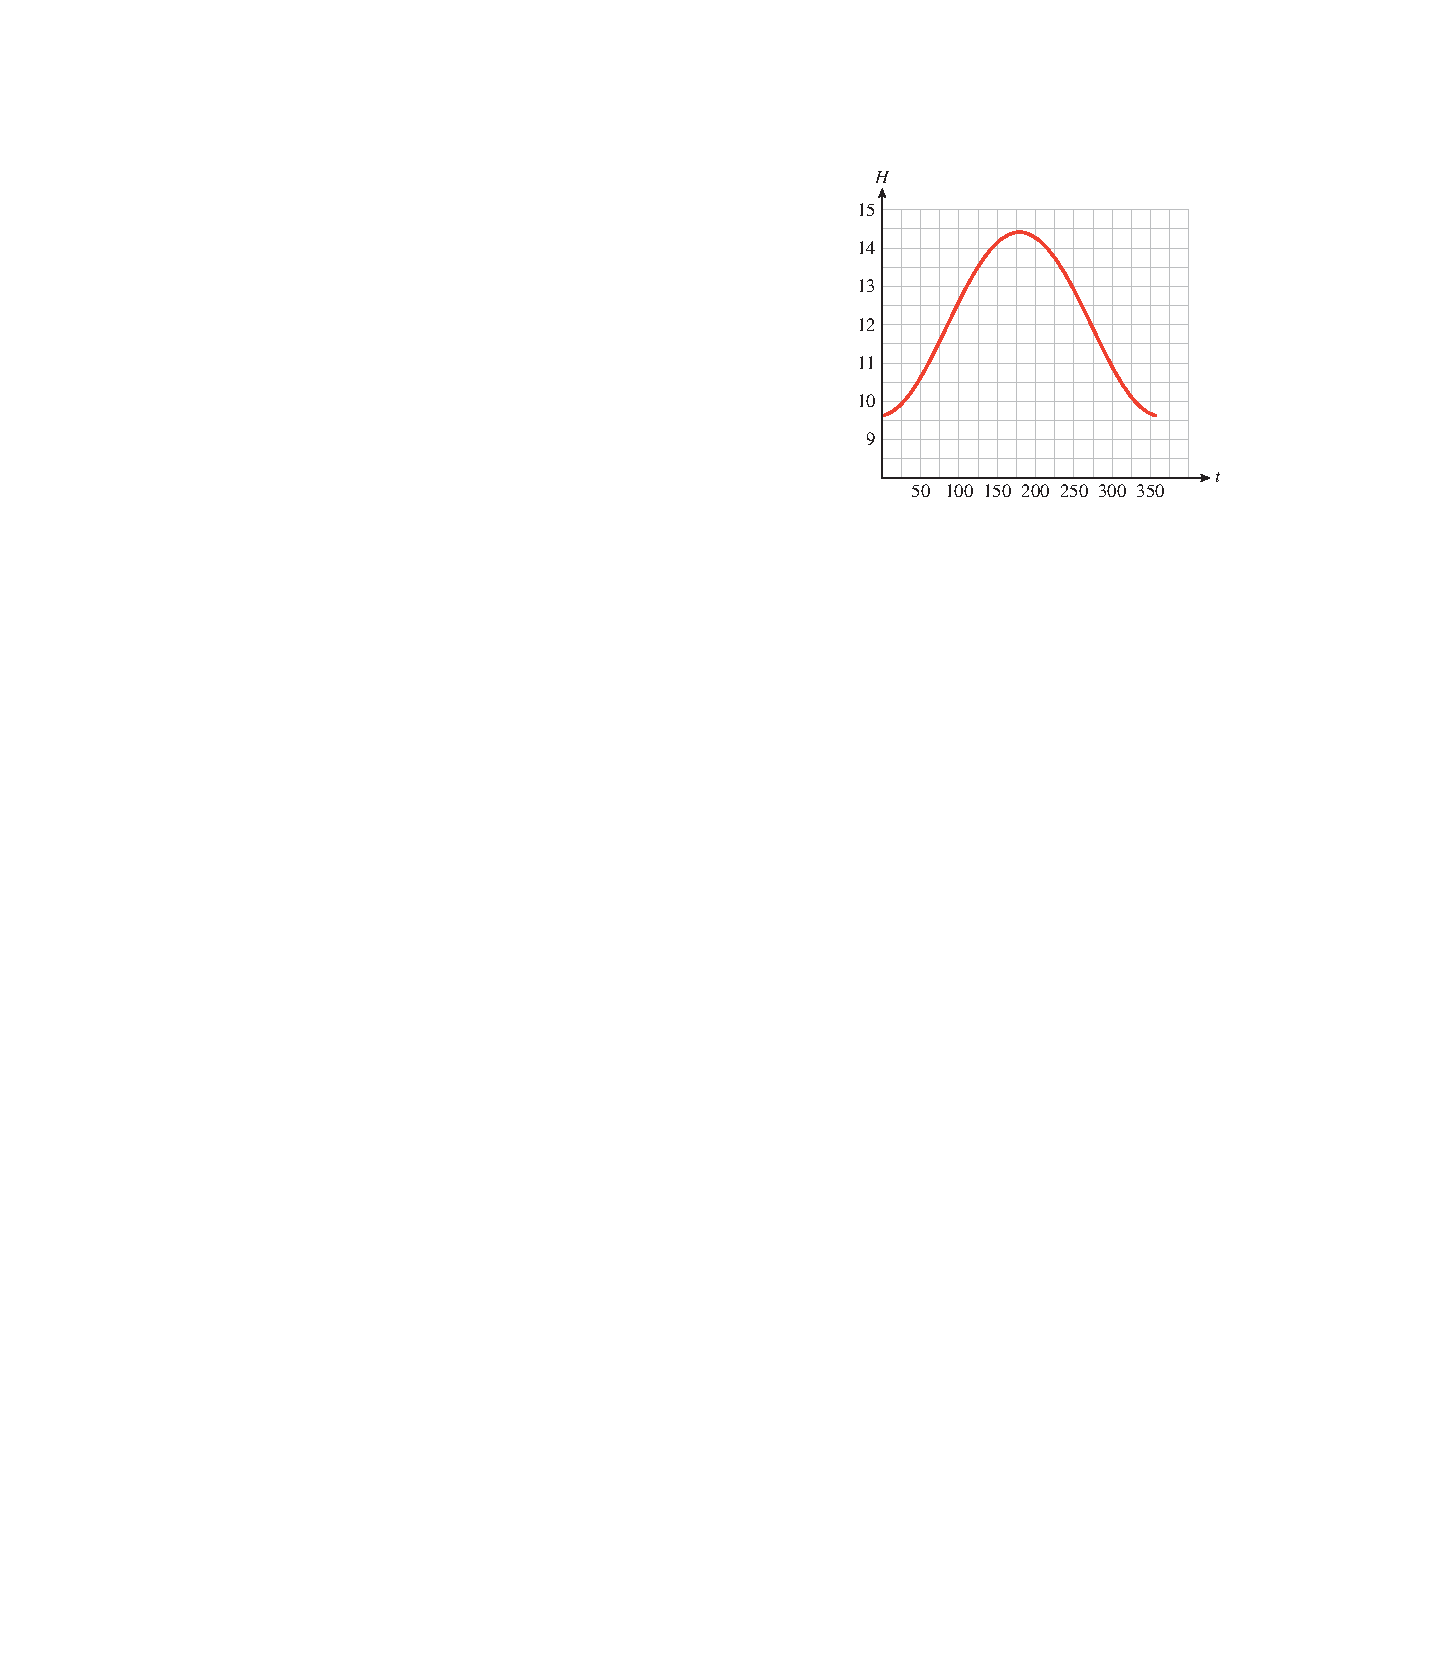
\includegraphics[width=\textwidth,]{images/fig-sun-hours.pdf}}% end body 
{\captionof{figure}{\label{fig-sun-hours}}
}% caption 
\popValignCaptionBottom
\end{figure}
\par\medskip\noindent%
\textbf{Solution.}\quad \leavevmode%
\begin{enumerate}[label=*\alph**]
\item\hypertarget{li-87}{}The input variable, \(t\), appears on the horizontal axis. The number of daylight hours, \(H\), is a function of the date. The output variable appears on the vertical axis.%
\item\hypertarget{li-88}{}The point on the curve where \(t = 150\) has \(H \approx 14.1\), so Peoria gets about 14.1 hours of daylight when \(t = 150\), which is at the end of May.%
\item\hypertarget{li-89}{}\(H = 12\) at the two points where \(t \approx 85\) (in late March) and \(t \approx 270\) (late September).%
\item\hypertarget{li-90}{}The maximum value of 14.4 hours occurs on the longest day of the year, when \(t \approx 170\), about three weeks into June. The minimum of 9.6 hours occurs on the shortest day, when \(t \approx 355\), about three weeks into December.%
\end{enumerate}
\end{example}
\begin{exercise}\label{exercise-LA-marathon}
\hyperref[fig-LA-marathon]{Figure~\ref{fig-LA-marathon}}  shows the elevation in feet, \(a\), of the Los Angeles Marathon course at a distance \(d\) miles into the race. (Source: \emph{Los Angeles Times}, March 3, 2005)
    \leavevmode%
\begin{figure}
\centering
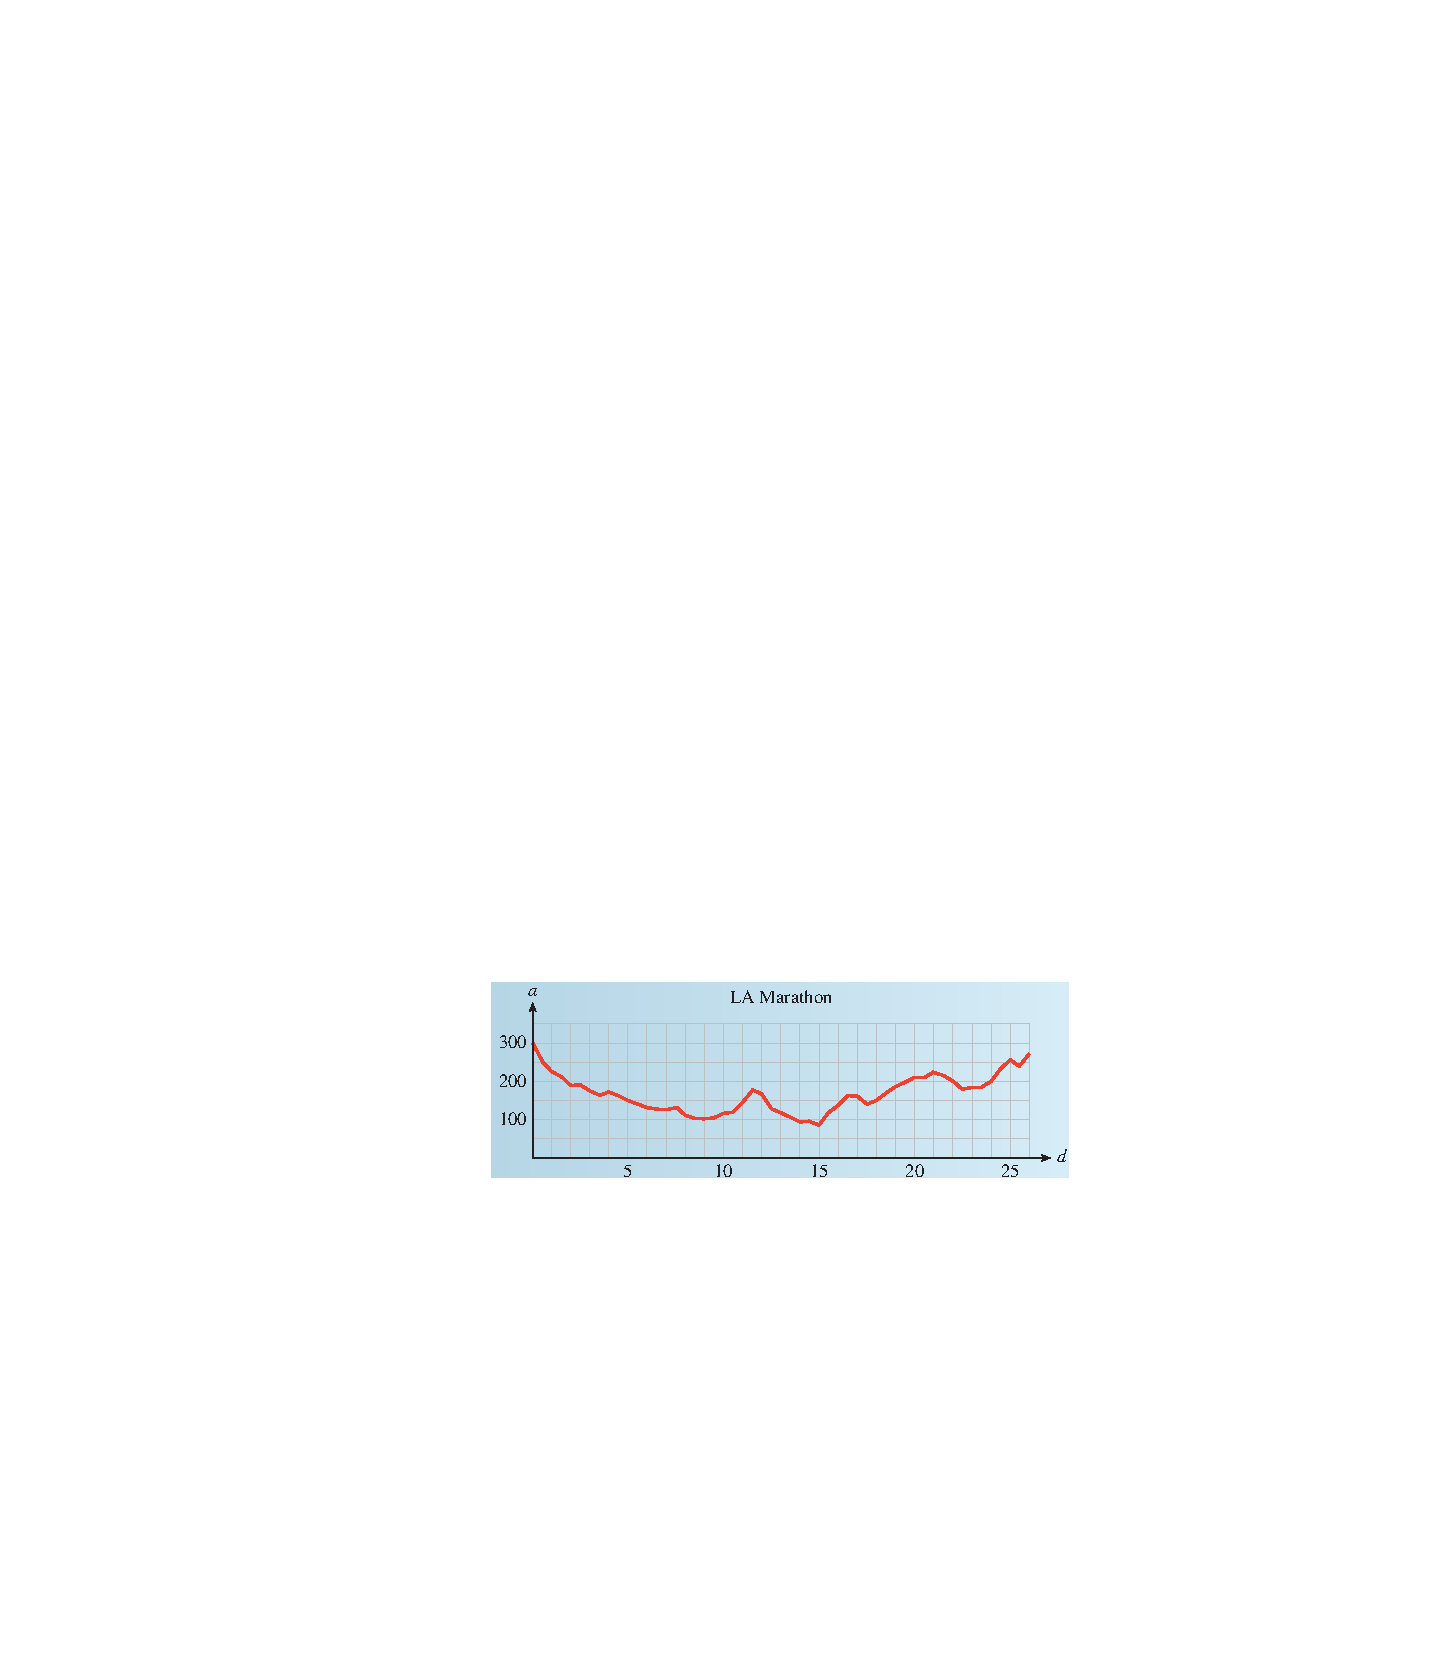
\includegraphics[width=0.100\textwidth,]{images/fig-LA-marathon.pdf}\caption{\label{fig-LA-marathon}}
\end{figure}
\leavevmode%
\begin{enumerate}[label=*\alph**]
\item\hypertarget{li-91}{}Which variable is the input, and which is the output?%
\item\hypertarget{li-92}{}What is the elevation at mile 20?%
\item\hypertarget{li-93}{}At what distances is the elevation 150 feet?%
\item\hypertarget{li-94}{}What are the maximum and minimum values of \(a\), and when do these values occur?%
\item\hypertarget{li-95}{}The runners pass by the Los Angeles Coliseum at about 4.2 miles into the race. What is the elevation there?%
\end{enumerate}
\end{exercise}
\typeout{************************************************}
\typeout{Subsection 1.2.4 Functions Defined by Equations}
\typeout{************************************************}
\subsection[Functions Defined by Equations]{Functions Defined by Equations}\label{subsection-9}
 illustrates a function defined by an equation.%
\begin{example}[]\label{example-falling-book}
As of 2016,  One World Trade Center in New York City is the nation’s tallest building, at 1776 feet. If an algebra book is dropped from the top of the Sears Tower, its height above the ground after \(t\) seconds is given by the equation \begin{equation*}h = 1776 − 16t^2\end{equation*} Thus, after \(\alert{1}\) second the book’s height is \begin{equation*}h = 1776 − 16(\alert{1})^2 = 1760 \text{ feet}\end{equation*} After \(\alert{2}\) seconds its height is \begin{equation*}h = 1776 − 16(\alert{2})^2 = 1712 \text{ feet}\end{equation*} For this function, \(t\) is the input variable and \(h\) is the output variable. For any value of \(t\), a unique value of \(h\) can be determined from the equation for \(h\). We say that \(h\) \emph{is a function of} \(t\).%
\end{example}
\begin{exercise}\label{exercise-11}
Write an equation that gives the volume, \(V\), of a sphere as a function of its radius, \(r\).
\end{exercise}
\begin{remark}[
\includegraphics[width=0.8\textwidth,]{images/icon-GC.pdf}Making a Table of Values with a Calculator]\label{remark-3}
We can use a graphing calculator to make a table of values for a function defined by an equation. For the function in \hyperref[example-falling-book]{Example~\ref{example-falling-book}}, 
    \begin{equation*}h = 1776 − 16t^2\end{equation*}
    we begin by entering the equation: Press the \lstinline?Y=? key, clear out any other equations, and define \(Y_1 = 1776 − 16X^2.\)%
\par
Next, we choose the \(x\)-values for the table. Press \lstinline?2nd?\lstinline?WINDOW? to access the TblSet (Table Setup) menu and set it to look like \hyperref[fig-TblSetup]{Figure~\ref{fig-TblSetup}}. This setting will give us an initial x-value of 0 \((TblStart = 0)\) and an increment of one unit in the x-values, \((\Delta Tbl = 1)\). It also fills in values of both variables automatically. Now press \lstinline?2nd? \lstinline?GRAPH? to see the table of values, as shown in \hyperref[fig-GC-table]{Figure~\ref{fig-GC-table}}. From this table, we can check the heights we found in \hyperref[example-falling-book]{Example~\ref{example-falling-book}}. Now try making a table of values with \(TblStart = 0\) and \(\Delta Tbl = 0.5\). Use the \lstinline?↑? and \lstinline?↓? arrow keys to scroll up and down the table.
    %
\leavevmode%
\begin{figure}
\centering
\pushValignCaptionBottom[b]{minipage}{.50\textwidth}{%
\centering% horizontal alignment 
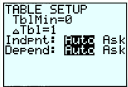
\includegraphics[width=\textwidth,]{images/fig-TblSetup.pdf}}% end body 
{\captionof{figure}{\label{fig-TblSetup}}
}% caption 
\pushValignCaptionBottom[b]{minipage}{.50\textwidth}{%
\centering% horizontal alignment 
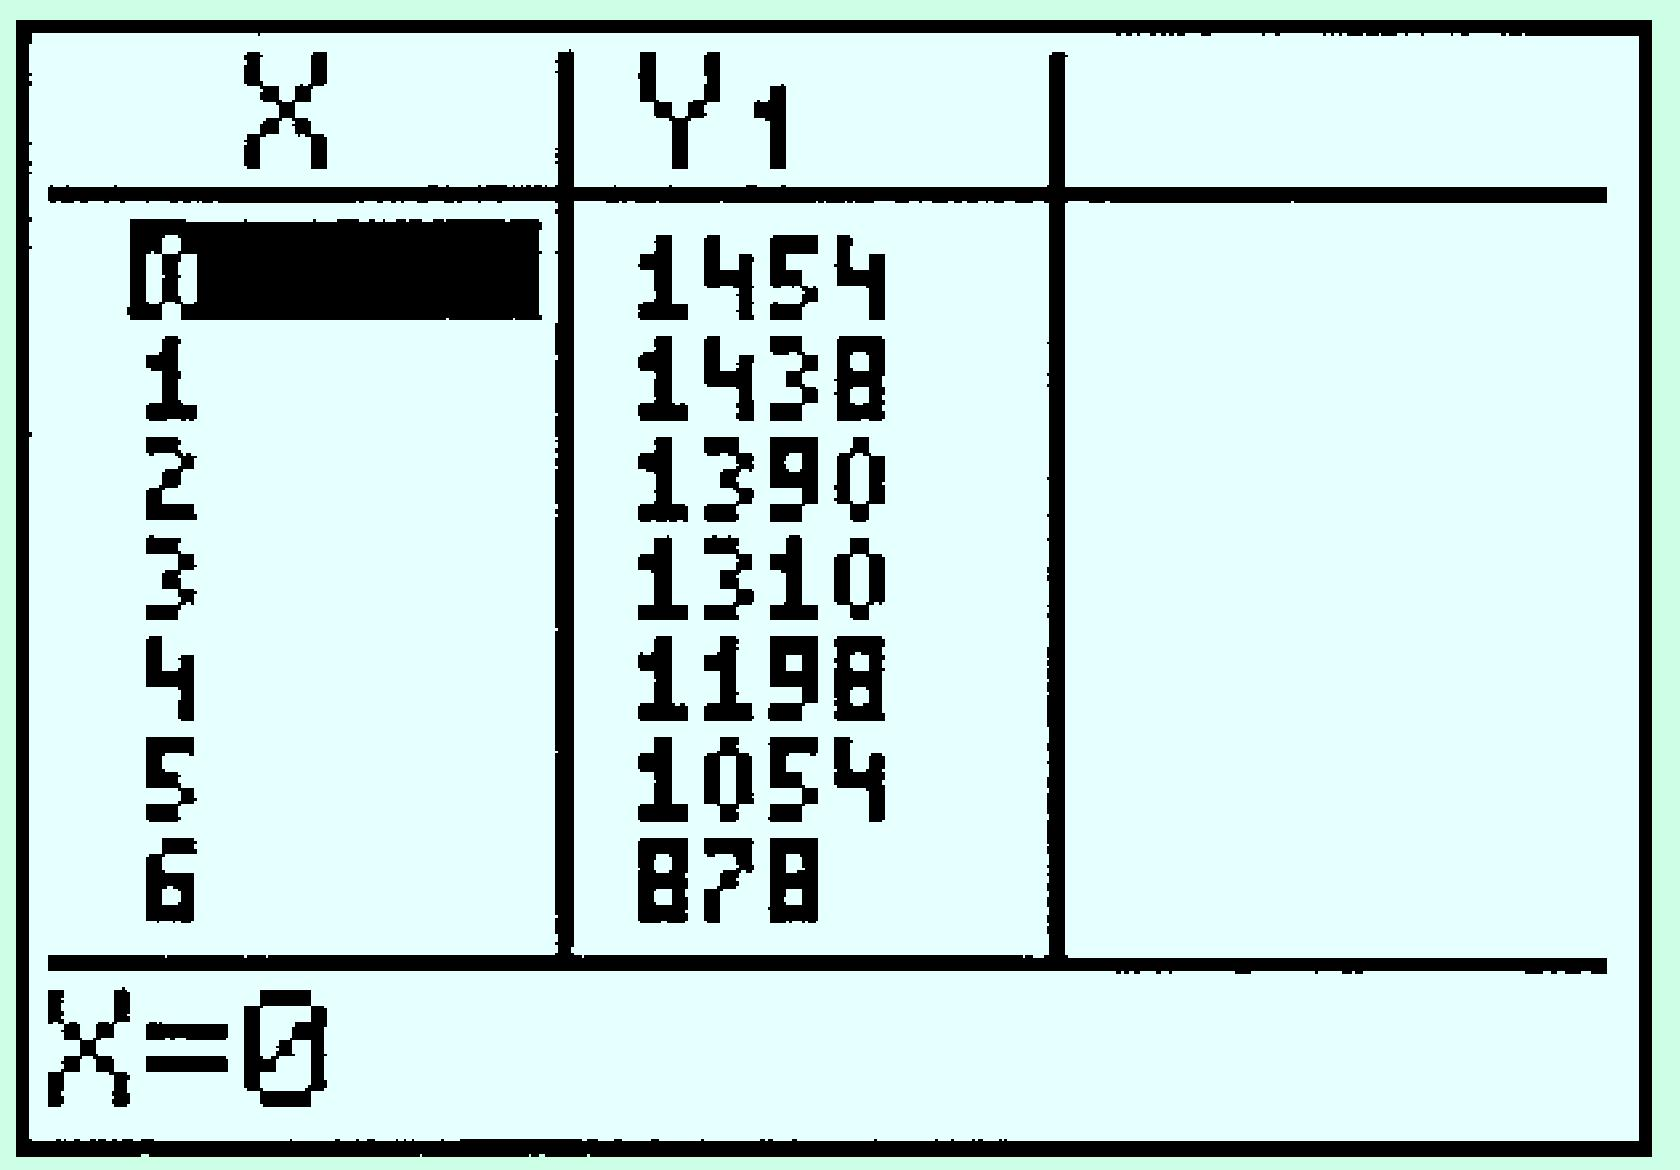
\includegraphics[width=\textwidth,]{images/fig-GC-table.pdf}}% end body 
{\captionof{figure}{\label{fig-GC-table}}
}% caption 
\popValignCaptionBottom
\end{figure}
\end{remark}
\typeout{************************************************}
\typeout{Subsection 1.2.5 Function Notation}
\typeout{************************************************}
\subsection[Function Notation]{Function Notation}\label{subsection-10}
There is a convenient notation for discussing functions. First, we choose a letter, such as \(f\), \(g\), or \(h\) (or \(F\), \(G\), or \(H\)), to name a particular function. (We can use any letter, but these are
the most common choices.) For instance, in \hyperref[example-falling-book]{Example~\ref{example-falling-book}}, the height, \(h\), of a falling algebra book is a function of the elapsed time, \(t\). We might call this function \(f\). In other words, \(f\) is the name of the relationship between the variables \(h\) and \(t\). We write 
\begin{equation*}h = f (t)\end{equation*}
which means "\(h\) is a function of \(t\), and \(f\) is the name of the function."%
\par
The new symbol \(f(t)\), read "\(f\) of \(t\)," is another name for the height, \(h\). The parentheses in the symbol \(f(t)\) do not indicate multiplication. (It would not make sense to multiply the name of a function by a variable.) Think of the symbol \(f(t)\) as a single variable that represents
the output value of the function.%
\par
With this new notation we may write
\begin{equation*}h = f (t) = 1776 − 16t^2\end{equation*}
or just
\begin{equation*}f (t) = 1776 − 16t^2\end{equation*}
instead of
\begin{equation*}h = 1776 − 16t^2\end{equation*}
to describe the function.%
\par
Perhaps it seems complicated to introduce a new symbol for \(h\), but the notation \(f(t)\) is very useful for showing the correspondence between specific values of the variables \(h\) and \(t\).
%
\begin{example}[]\label{example-falling-book-2}
In \hyperref[example-falling-book]{Example~\ref{example-falling-book}}, the height of an algebra book dropped from the top of the Sears Tower is given by the equation
    \begin{equation*}h = 1776 − 16t^2\end{equation*}
We see that%
\leavevmode%
\begin{table}
\centering
\begin{tabular}{l}
when \(t=1\)&&\(h=1760\)\tabularnewline[0pt]
when \(t=2\)&&\(h=1712\)
\end{tabular}
\end{table}
\par
Using function notation, these relationships can be expressed more concisely as%
\leavevmode%
\begin{table}
\centering
\begin{tabular}{l}
\(f(1)=1760\)& and &\(f(2)=1712\)
\end{tabular}
\end{table}
\par
which we read as "\(f\) of 1 equals 1760" and "\(f\) of 2 equals 1712." The values for the input variable, \(t\), appear \emph{inside} the parentheses, and the values for the output variable, \(h\), appear on the other side of the equation.%
\end{example}
\par
Remember that when we write \(y = f(x)\), the symbol \(f(x)\) is just another name for the output variable.%
\typeout{************************************************}
\typeout{Paragraphs  Function Notation}
\typeout{************************************************}
\paragraph[Function Notation]{Function Notation}\label{paragraphs-6}
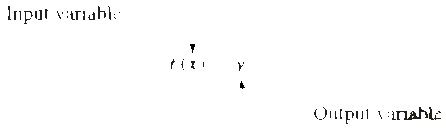
\includegraphics[width=0.70\textwidth,]{images/fig-Function-Notation.pdf}\begin{exercise}\label{exercise-12}
Let \(F\) be the name of the function defined by the graph in \hyperref[example-sun-hours]{Example~\ref{example-sun-hours}}, the number of hours of daylight in Peoria.
\leavevmode%
\begin{enumerate}[label=*\alph**]
\item\hypertarget{li-96}{}Use function notation to state that \(H\) is a function of \(t\).%
\item\hypertarget{li-97}{}What does the statement \(F(15) = 9.7\) mean in the context of the problem?%
\end{enumerate}
\end{exercise}
\typeout{************************************************}
\typeout{Subsection 1.2.6 Evaluating a Function}
\typeout{************************************************}
\subsection[Evaluating a Function]{Evaluating a Function}\label{subsection-11}

    Finding the value of the output variable that corresponds to a particular value of the input variable is called \terminology{evaluating the function}.
%
\begin{example}[]\label{example-postage2}
Let \(g\) be the name of the postage function defined by \hyperref[table-postage]{Table~\ref{table-postage}}  in \hyperref[example-functions]{Example~\ref{example-functions}}. Find \(g(1)\), \(g(3)\), and \(g(6.75\)).%
\par\medskip\noindent%
\textbf{Solution.}\quad According to the table,
    \leavevmode%
\begin{table}
\centering
\begin{tabular}{l}
when \(w=1\),&&\(p=0.47\)& so &\(g(1)=0.47\)\tabularnewline[0pt]
when \(w=3\),&&\(p=0.89\)& so &\(g(3)=0.89\)\tabularnewline[0pt]
when \(w=6.75\),&&\(p=1.73\)& so &\(g(6.75)=1.73\)
\end{tabular}
\end{table}

     Thus, a letter weighing 1 ounce costs \textdollar{}0.47 to mail, a letter weighing 3 ounces costs \textdollar{}0.89, and a letter weighing 6.75 ounces costs \textdollar{}1.73.%
\end{example}
\begin{exercise}\label{exercise-heart-rate}

    When you exercise, your heart rate should increase until it reaches your target heart rate. The table shows target heart rate, \(r = f(a)\), as a function of age. 
    \leavevmode%
\begin{table}
\centering
\begin{tabular}{AcAcAcAcAcAcAcAcAcAcAcAcA}\hrulethick
\(a\)%
&20%
&25%
&30%
&35%
&40%
&45%
&50%
&55%
&60%
&65%
&70%
\tabularnewline\hrulethin
\(r\)%
&150%
&146%
&142%
&139%
&135%
&131%
&127%
&124%
&120%
&116%
&112%
\tabularnewline\hrulethin
\end{tabular}
\end{table}
\leavevmode%
\begin{enumerate}[label=*\alph**]
\item\hypertarget{li-98}{}Find \(f(25)\) and \(f(50)\).%
\item\hypertarget{li-99}{}Find a value of \(a\) for which \(f(a) = 135\).%
\end{enumerate}
\end{exercise}
\par
If a function is described by an equation, we simply substitute the given input value into the equation to find the corresponding output, or function value.%
\begin{example}[]\label{example-evaluate-function}
The function \(H\) is defined by \(H=f(s) = \frac{\sqrt{s+3}}{s}\). Evaluate the function at the following values.%
\leavevmode%
\begin{enumerate}[label=*\alph**]
\item\hypertarget{li-100}{}\(s=6\)%
\item\hypertarget{li-101}{}\(s=-1\)%
\end{enumerate}
\par\medskip\noindent%
\textbf{Solution.}\quad \leavevmode%
\begin{enumerate}[label=*\alph**]
\item\hypertarget{li-102}{}\(f(\alert{6})=\frac{\sqrt{\alert{6}+3}}{\alert{6}}=
            \frac{\sqrt{9}}{6}=\frac{3}{6}=\frac{1}{2}\). Thus, \(f(6)=\frac{1}{2}\).%
\item\hypertarget{li-103}{}\(f(\alert{-1})=\frac{\sqrt{\alert{-1}+3}}{\alert{-1}}=
            \frac{\sqrt{2}}{-1}=-\sqrt{2}\). Thus, \(f(-1)=-\sqrt{2}\).%
\end{enumerate}
\end{example}
\begin{exercise}\label{exercise-function-notation}

    Complete the table displaying ordered pairs for the function \(f(x) = 5 − x^3\). Evaluate the function to find the corresponding \(f(x)\)-value for each value of \(x\).
    \leavevmode%
\begin{table}
\centering
\begin{tabular}{AcAcAlA}\hrulethick
\(x\)%
&\(f(x)\)%
&\tabularnewline\hrulethin
\(-2\)&\(\)&\(f(\alert{-2})=5-(\alert{-2})^3=~\) \tabularnewline\hrulethin
\(0\)&\(\)&\(f(\alert{0})=5-\alert{0}^3=\)\tabularnewline\hrulethin
\(1\)&\(\)&\(f(\alert{1})=5-\alert{1}^3=\)\tabularnewline\hrulethin
\(3\)&\(\)&\(f(\alert{3})=5-\alert{3}^3=\)\tabularnewline\hrulethin
\end{tabular}
\end{table}
\end{exercise}
\begin{remark}[
\includegraphics[width=0.8\textwidth,]{images/icon-GC.pdf}Evaluating a Function]\label{remark-4}
We can use the table feature on a graphing calculator to evaluate functions. Consider the function of \hyperref[exercise-function-notation]{Exercise~\ref{exercise-function-notation}}, \(f(x) = 5 − x^3\).%
\par
Press 
\includegraphics[width=0.6\textwidth,]{images/y-equals.pdf}, clear any old functions, and enter
    \begin{equation*}Y_1 = 5−X \text{^} 3\end{equation*}
    Then press TblSet (,\lstinline?2nd? \lstinline?WINDOW?) and choose Ask after Indpnt, as shown in \hyperref[fig-TblSetup2]{Figure~\ref{fig-TblSetup2}}, and press \lstinline?ENTER?. This setting allows you to enter any \(x\)-values you like. Next, press TABLE (using \lstinline?2nd? \lstinline?GRAPH?). To follow \hyperref[exercise-function-notation]{Exercise~\ref{exercise-function-notation}}, key in \lstinline?(-)? 2 \lstinline?ENTER? for the \(x\)-value, and the calculator will fill in the \(y\)-value. Continue by entering 0, 1, 3, or any other \(x\)-values you choose. One such table is shown in \hyperref[fig-GC-table2]{Figure~\ref{fig-GC-table2}}. If you would like to evaluate a new function, you do not have to return to the \lstinline?Y=? screen. Use the \lstinline?→? and \lstinline?↑? arrow keys to highlight \(Y_1\) at the top of the second column. The definition of \(Y_1\) will appear at the bottom of the display, as shown in \hyperref[fig-GC-table2]{Figure~\ref{fig-GC-table2}}. You can key in a new definition here, and the second column will be updated automatically to show the \(y\)-values of the new function.
    \leavevmode%
\begin{figure}
\centering
\pushValignCaptionBottom[b]{minipage}{.50\textwidth}{%
\centering% horizontal alignment 
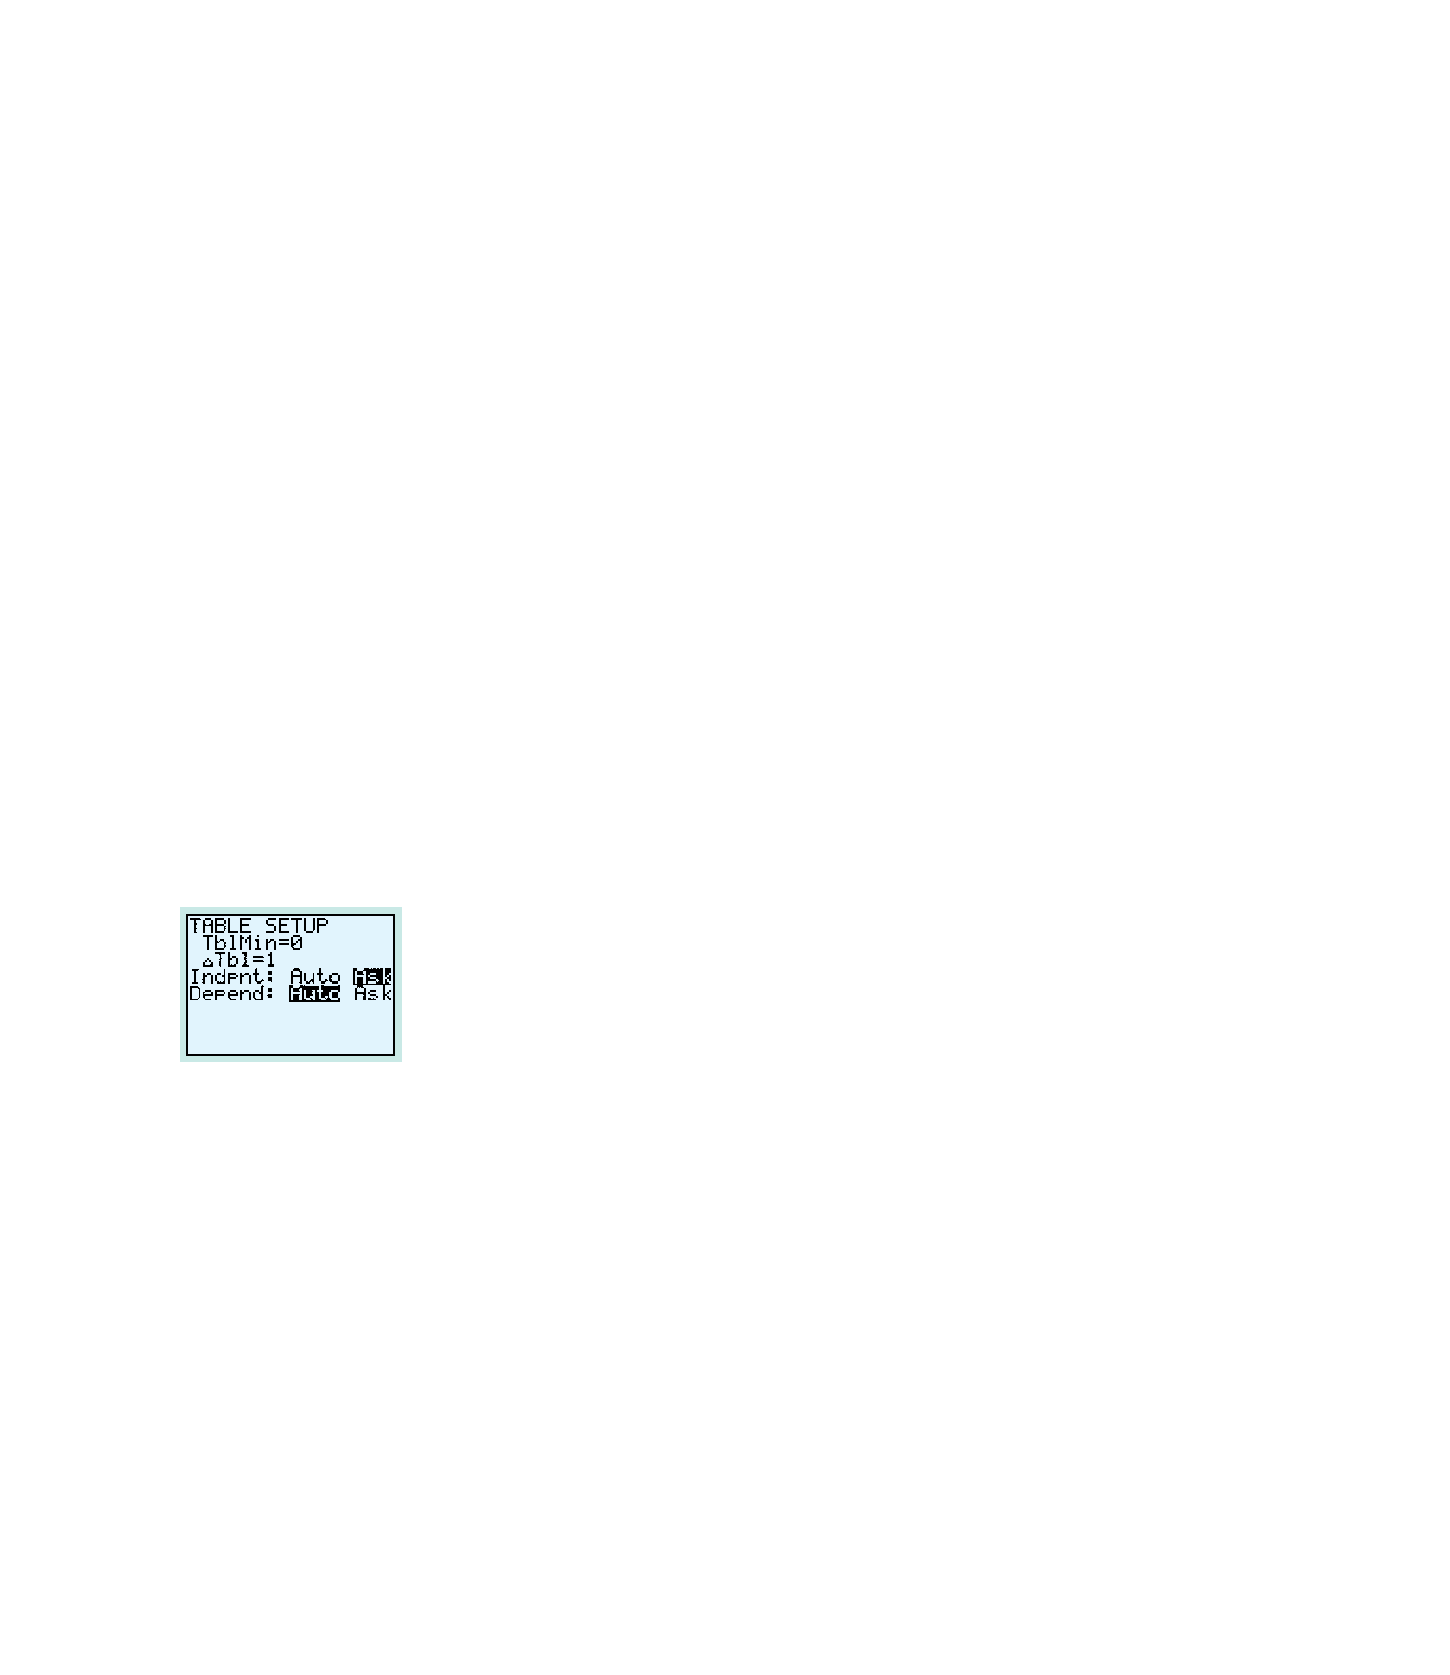
\includegraphics[width=\textwidth,]{images/fig-TblSetup2.pdf}}% end body 
{\captionof{figure}{\label{fig-TblSetup2}}
}% caption 
\pushValignCaptionBottom[b]{minipage}{.50\textwidth}{%
\centering% horizontal alignment 
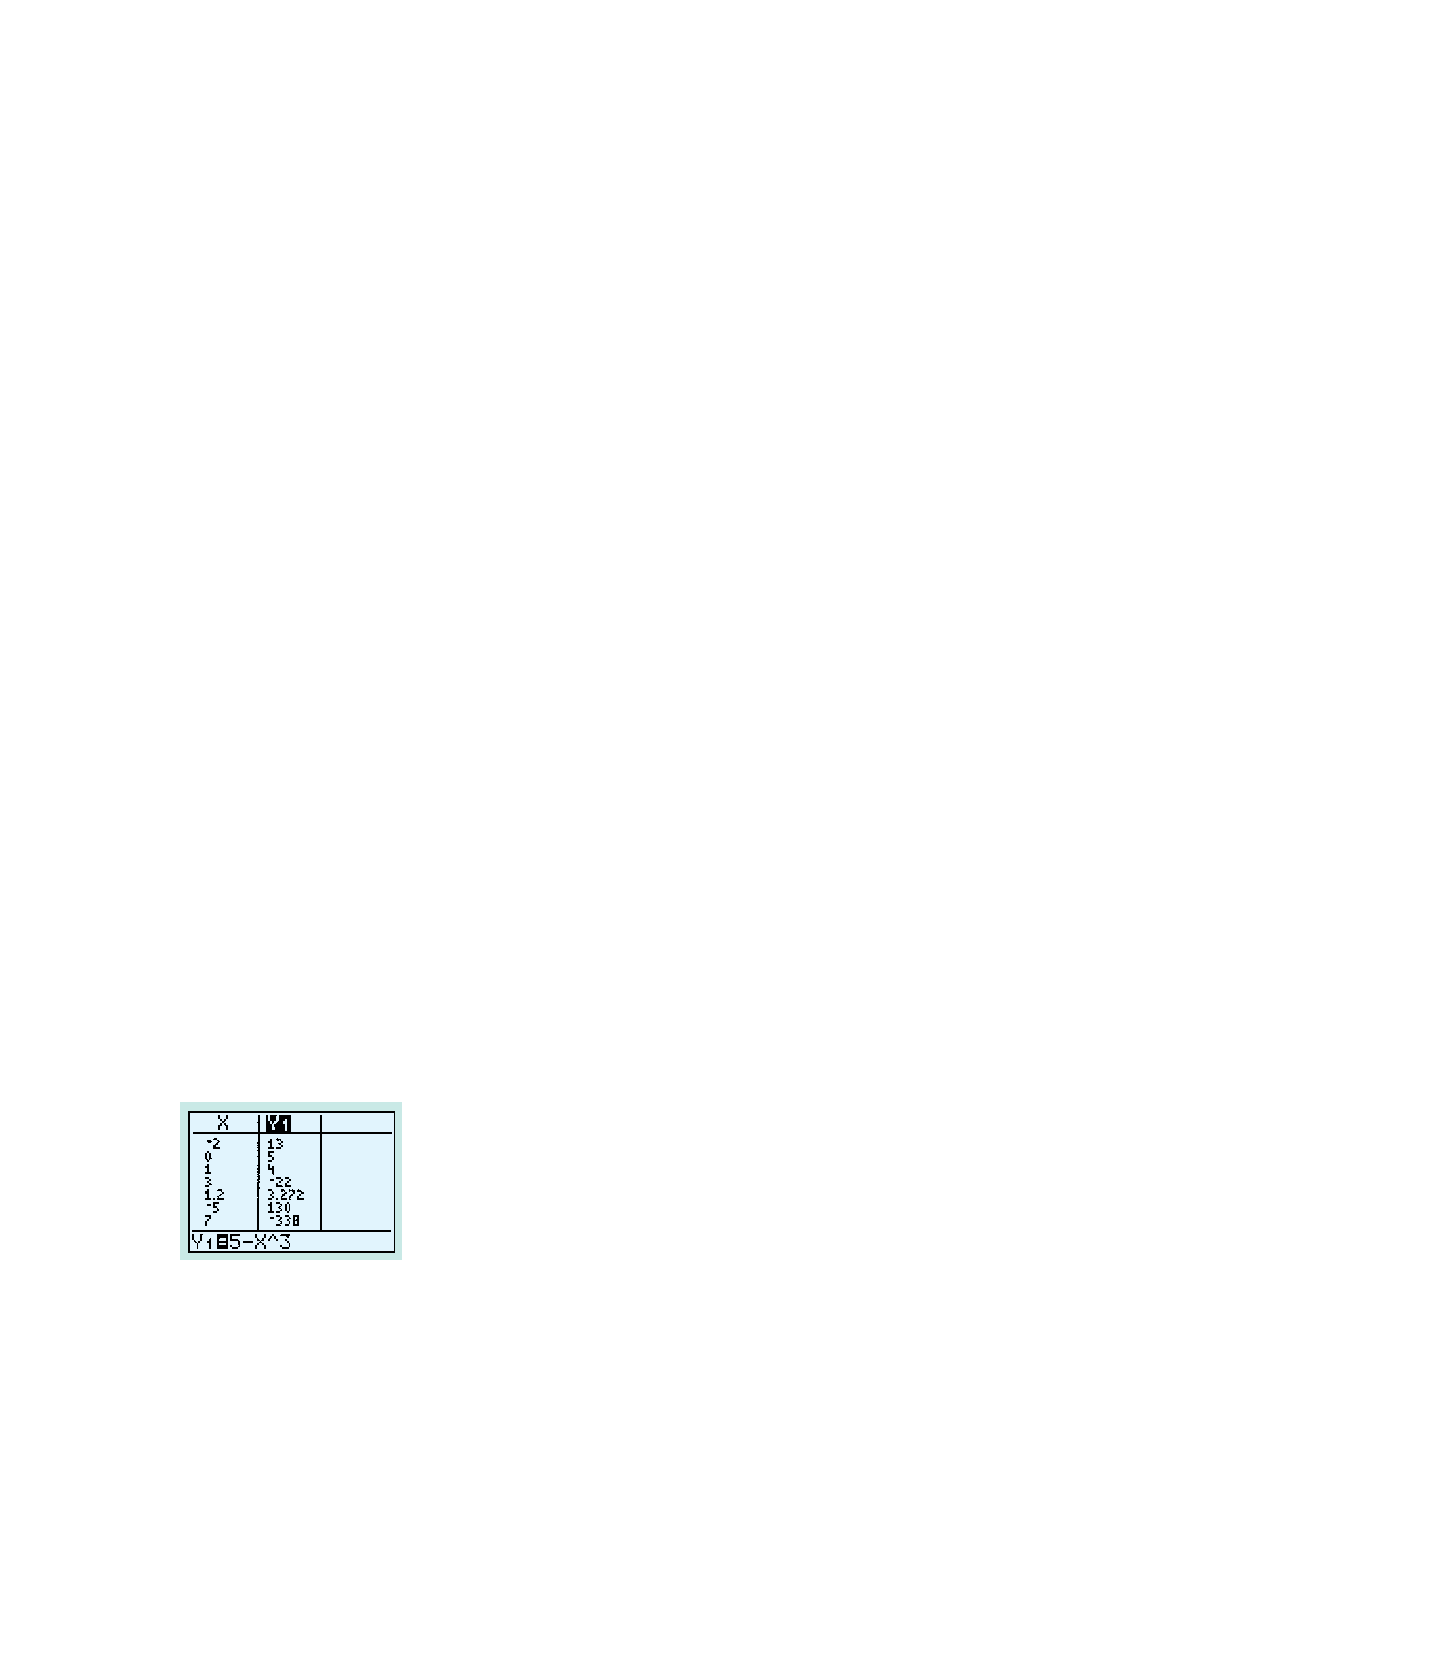
\includegraphics[width=\textwidth,]{images/fig-GC-table2.pdf}}% end body 
{\captionof{figure}{\label{fig-GC-table2}}
}% caption 
\popValignCaptionBottom
\end{figure}

    %
\end{remark}
\par

    To simplify the notation, we sometimes use the same letter for the output variable and
for the name of the function. In the next example, \(C\) is used in this way.
%
\begin{example}[]\label{example-function-notation-abuse}
TrailGear decides to market a line of backpacks. The cost, \(C\), of manufacturing backpacks is a function of the number, \(x\), of backpacks produced, given by the equation 
    \begin{equation*}C(x) = 3000 + 20x\end{equation*}
    where \(C(x)\) is measured in dollars. Find the cost of producing 500 backpacks.%
\par\medskip\noindent%
\textbf{Solution.}\quad To find the value of \(C\) that corresponds to \(x = \alert{500}\), evaluate \(C(500)\).
    \begin{equation*}C(\alert{500}) = 3000 + 20(\alert{500}) = 13,000\end{equation*}
    The cost of producing 500 backpacks is \textdollar{}13,000.\end{example}
\begin{exercise}\label{exercise-sphere-volume}

        The volume of a sphere of radius \(r\) centimeters is given by
        \begin{equation*}V = V(r) = \frac{4}{3}\pi r^3\end{equation*}
        Evaluate \(V(10)\) and explain what it means.
    \end{exercise}
\typeout{************************************************}
\typeout{Subsection 1.2.7 Operations with Function Notation}
\typeout{************************************************}
\subsection[Operations with Function Notation]{Operations with Function Notation}\label{subsection-12}
Sometimes we need to evaluate a function at an algebraic expression rather than at a
specific number.%
\begin{example}[]\label{example-backpacks}
TrailGear manufactures backpacks at a cost of
    \begin{equation*}C(x) = 3000 + 20x\end{equation*}
    for \(x\) backpacks. The company finds that the monthly demand for backpacks increases by 50% during the summer. The backpacks are produced at several small co-ops in different states.%
\leavevmode%
\begin{enumerate}[label=*\alph**]
\item\hypertarget{li-104}{}If each co-op usually produces \(b\) backpacks per month, how many should it produce during the summer months?\item\hypertarget{li-105}{}What costs for producing backpacks should the company expect during the summer?\end{enumerate}
\par\medskip\noindent%
\textbf{Solution.}\quad \leavevmode%
\begin{enumerate}[label=*\alph**]
\item\hypertarget{li-106}{}An increase of 50% means an additional 50% of the current production level, \(b\). Therefore, a co-op that produced \(b\) backpacks per month during the winter should increase production to \(b + 0.5b\), or \(1.5b\) backpacks per month in the summer.\item\hypertarget{li-107}{}The cost of producing \(1.5b\) backpacks will be
            \begin{equation*}C(\alert{1.5b}) = 3000 + 20(\alert{1.5b}) = 3000 + 30b\end{equation*}\end{enumerate}
\end{example}
\begin{exercise}\label{exercise-spherical-balloon}

        A spherical balloon has a radius of 10 centimeters.
        \leavevmode%
\begin{enumerate}[label=*\alph**]
\item\hypertarget{li-108}{}If we increase the radius by \(h\) centimeters, what will the new volume be?\item\hypertarget{li-109}{}If \(h = 2\), how much did the volume increase?\end{enumerate}
\end{exercise}
\begin{example}[]\label{example-evaluate-quadratic}
Evaluate the function \(f(x)=4x^2 − x + 5\) for the following expressions.%
\leavevmode%
\begin{enumerate}[label=*\alph**]
\item\hypertarget{li-110}{}\(x = 2h\)\item\hypertarget{li-111}{}\(x = a + 3\)\end{enumerate}
\par\medskip\noindent%
\textbf{Solution.}\quad \leavevmode%
\begin{enumerate}[label=*\alph**]
\item\hypertarget{li-112}{}~ %
\begin{align*}
                f(\alert{2h}) \&= 4(\alert{2h})^2−(\alert{2h}) + 5\textbackslash{}\textbackslash{}\&= 4(4h^2)−2h+5\textbackslash{}\textbackslash{}\&= 16h^2 − 2h + 5\textbackslash{}\textbackslash{} 
                \end{align*}\item\hypertarget{li-113}{}~ %
\begin{align*}
                f(\alert{a+3}) \&= 4(\alert{a+3})^2−(\alert{a+3})+5\textbackslash{}\textbackslash{}\&= 4(a^2+6a+9)−a-3+5\textbackslash{}\textbackslash{}\&= 4a^2+24a+36 − a + 2\textbackslash{}\textbackslash{}\&= 4a^2+23a + 38\textbackslash{}\textbackslash{} 
                \end{align*}\end{enumerate}
\end{example}
\typeout{************************************************}
\typeout{Paragraphs  CAUTION}
\typeout{************************************************}
\paragraph[CAUTION]{CAUTION}\label{paragraphs-7}
In \hyperref[example-evaluate-quadratic]{Example~\ref{example-evaluate-quadratic}}, notice that
\begin{equation*}f(2h) \ne 2 f(h)\end{equation*}
and
\begin{equation*}f(a + 3) \ne f(a) + f(3)\end{equation*}
To compute \(f(a) + f(3)\), we must first compute \(f(a)\) and \(f(3)\), then add them:
    \begin{align*}
        f(a)+f(3)\&= (4a^2−a+5)+(4\cdot 3^2−3+5) \textbackslash{}\textbackslash{}
                \&= 4a^2 − a + 43\textbackslash{}\textbackslash{} 
                \end{align*}
In general, it is not true that \(f(a + b) = f(a) + f(b)\). Remember that the parentheses in the expression \(f(x)\) do not indicate multiplication, so the distributive law does not apply to the expression \(f(a + b)\).%
\begin{exercise}\label{exercise-function-notation2}

    Let \(f(x) = x^3 − 1\) and evaluate each expression.
    \leavevmode%
\begin{enumerate}[label=*\alph**]
\item\hypertarget{li-114}{}\(f(2) + f(3)\)\item\hypertarget{li-115}{}\(f(2 + 3)\)\item\hypertarget{li-116}{}\(2 f(x) + 3\)\end{enumerate}
\end{exercise}
\typeout{************************************************}
\typeout{Section 1.3 Graphs of Functions}
\typeout{************************************************}
\section[Graphs of Functions]{Graphs of Functions}\label{graphs-of-functions}
\typeout{************************************************}
\typeout{Subsection 1.3.1 Reading Function Values from a Graph}
\typeout{************************************************}
\subsection[Reading Function Values from a Graph]{Reading Function Values from a Graph}\label{subsection-13}
The graph in \hyperref[fig-DJIA]{Figure~\ref{fig-DJIA}}  shows the Dow-Jones Industrial Average (the average value of the stock prices of 500 major companies) during the stock market correction of October 1987. The Dow-Jones Industrial Average (DJIA) is given as a function of time during the 8 days from October 15 to October 22; that is, \(f(t)\) is the DJIA recorded at noon on day \(t\).
%
\leavevmode%
\begin{figure}
\centering
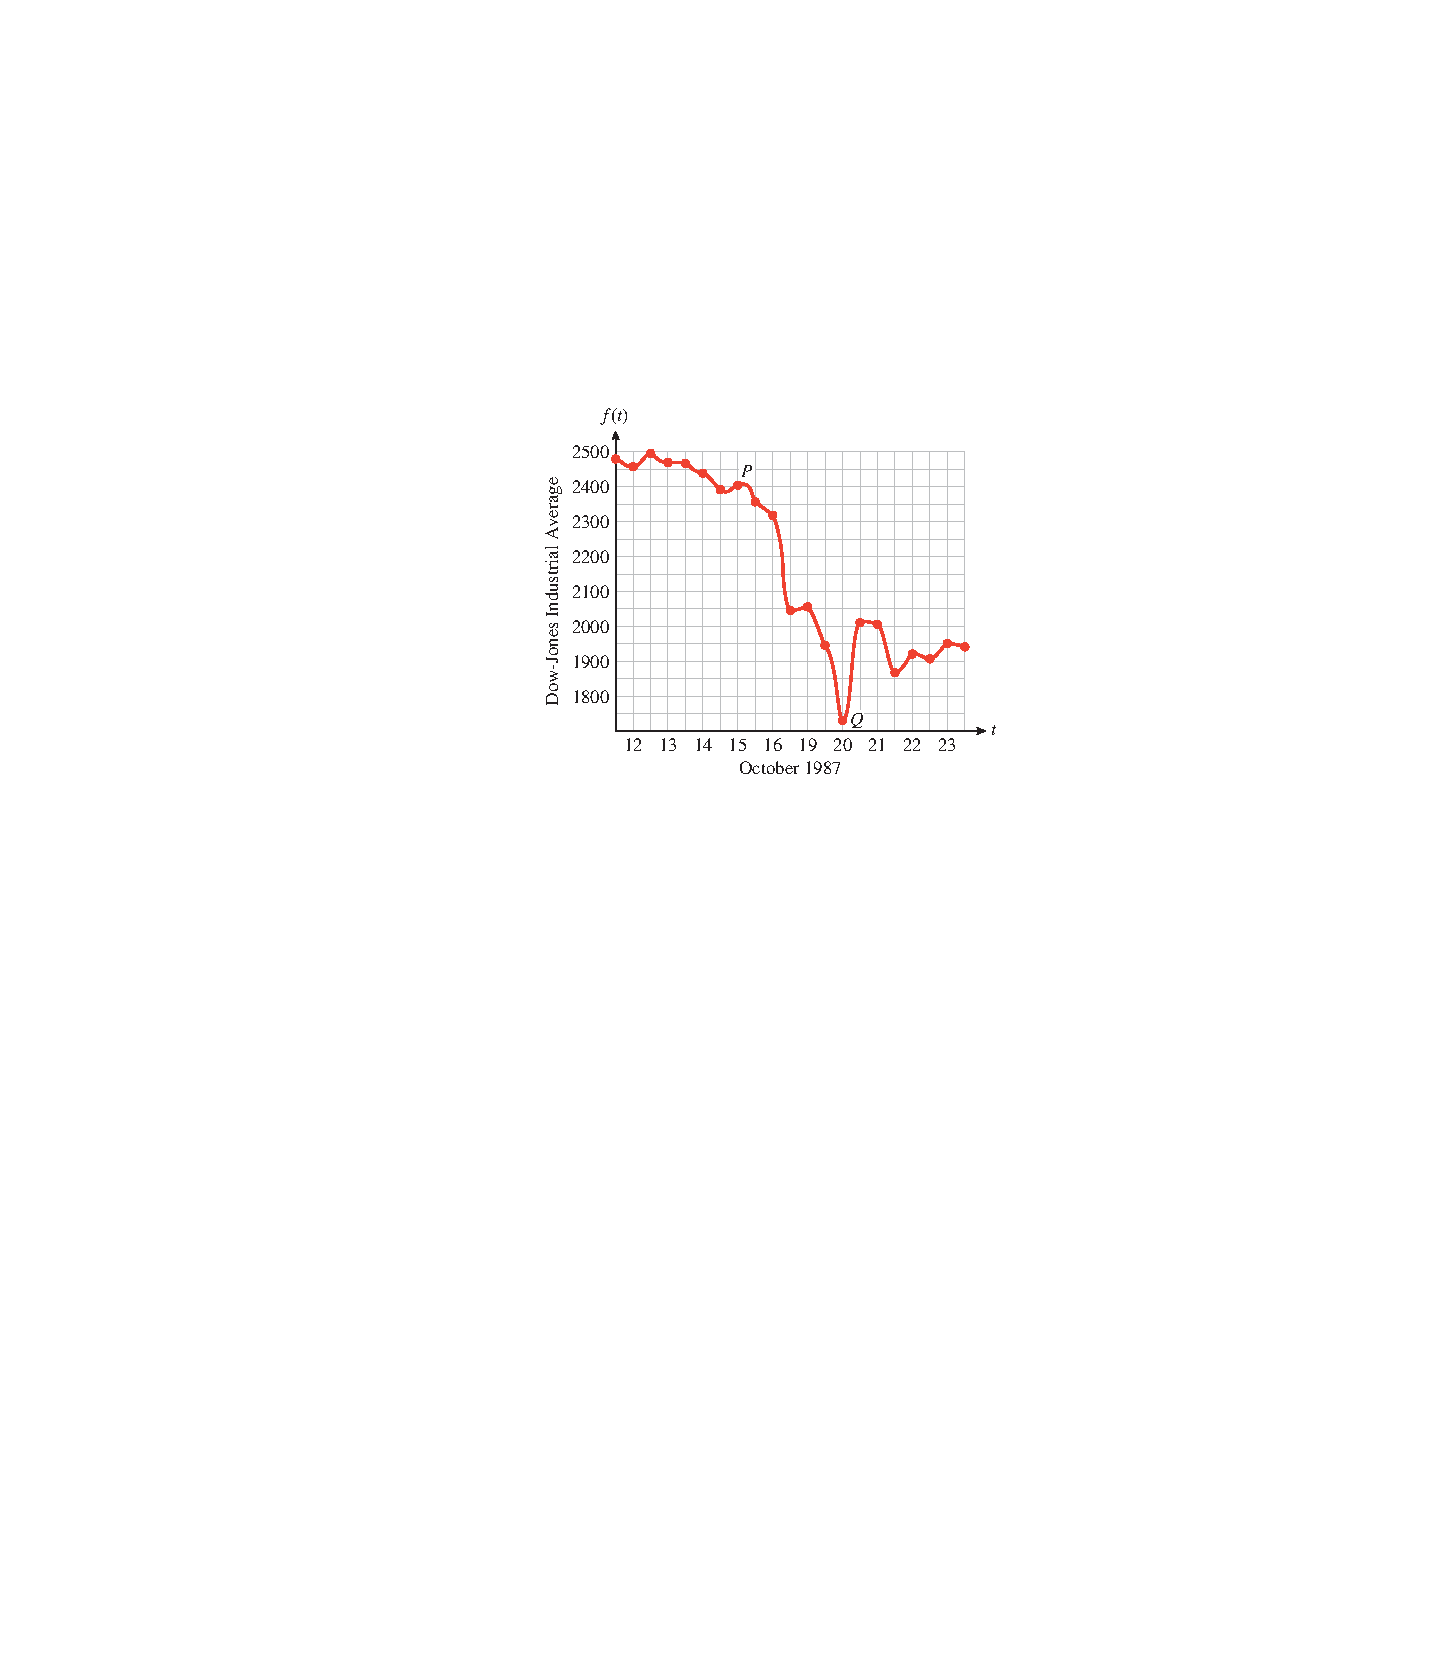
\includegraphics[width=0.80\textwidth,]{images/fig-DJIA.pdf}\caption{\label{fig-DJIA}}
\end{figure}
\par
The values of the input variable, time, are displayed on the horizontal axis, and the values of the output variable, DJIA, are displayed on the vertical axis. There is no formula that gives the DJIA for a particular day; but it is still a function, defined by its graph. The value of \(f(t)\) is specified by the vertical coordinate of the point with the given t-coordinate.
%
\begin{example}[]\label{example-DJIA}
\leavevmode%
\begin{enumerate}[label=*\alph**]
\item\hypertarget{li-117}{}The coordinates of point \(P\) in \hyperref[fig-DJIA]{Figure~\ref{fig-DJIA}} are \((15, 2412)\). What do the coordinates tell you about the function \(f\)?\item\hypertarget{li-118}{}If the DJIA was 1726 at noon on October 20, what can you say about the graph of \(f\)?\end{enumerate}
\par\medskip\noindent%
\textbf{Solution.}\quad \leavevmode%
\begin{enumerate}[label=*\alph**]
\item\hypertarget{li-119}{}The coordinates of point P tell us that \(f(15) = 2412\), so the DJIA was 2412 at noon on October 15.\item\hypertarget{li-120}{}We can say that \(f(20) = 1726\), so the point \((20, 1726)\) lies on the graph of \(f\). This point is labeled \(Q\) in \hyperref[fig-DJIA]{Figure~\ref{fig-DJIA}}.\end{enumerate}
\end{example}
\par
Thus, the coordinates of each point on the graph of the function represent a pair of corresponding
values of the two variables. In general, we can make the following statement.%
\typeout{************************************************}
\typeout{Paragraphs  Graph of a Function}
\typeout{************************************************}
\paragraph[Graph of a Function]{Graph of a Function}\label{paragraphs-8}
The point \((a, b)\) lies on the graph of the function \(f\) if and only if \(f(a)=b\).
%
\begin{example}[]\label{example-function-graph}
\hyperref[fig-function]{Figure~\ref{fig-function}} shows the graph of a function \(g\).
    \leavevmode%
\begin{enumerate}[label=*\alph**]
\item\hypertarget{li-121}{}Find \(g(−2)\) and \(g(5)\).\item\hypertarget{li-122}{}For what value(s) of \(t\) is \(g(t) = −2\)?\item\hypertarget{li-123}{}What is the largest, or maximum, value of \(g(t)\)? For what value of \(t\) does the function take on its maximum value?\item\hypertarget{li-124}{}On what intervals is \(g\) increasing?\end{enumerate}
%
\leavevmode%
\begin{figure}
\centering
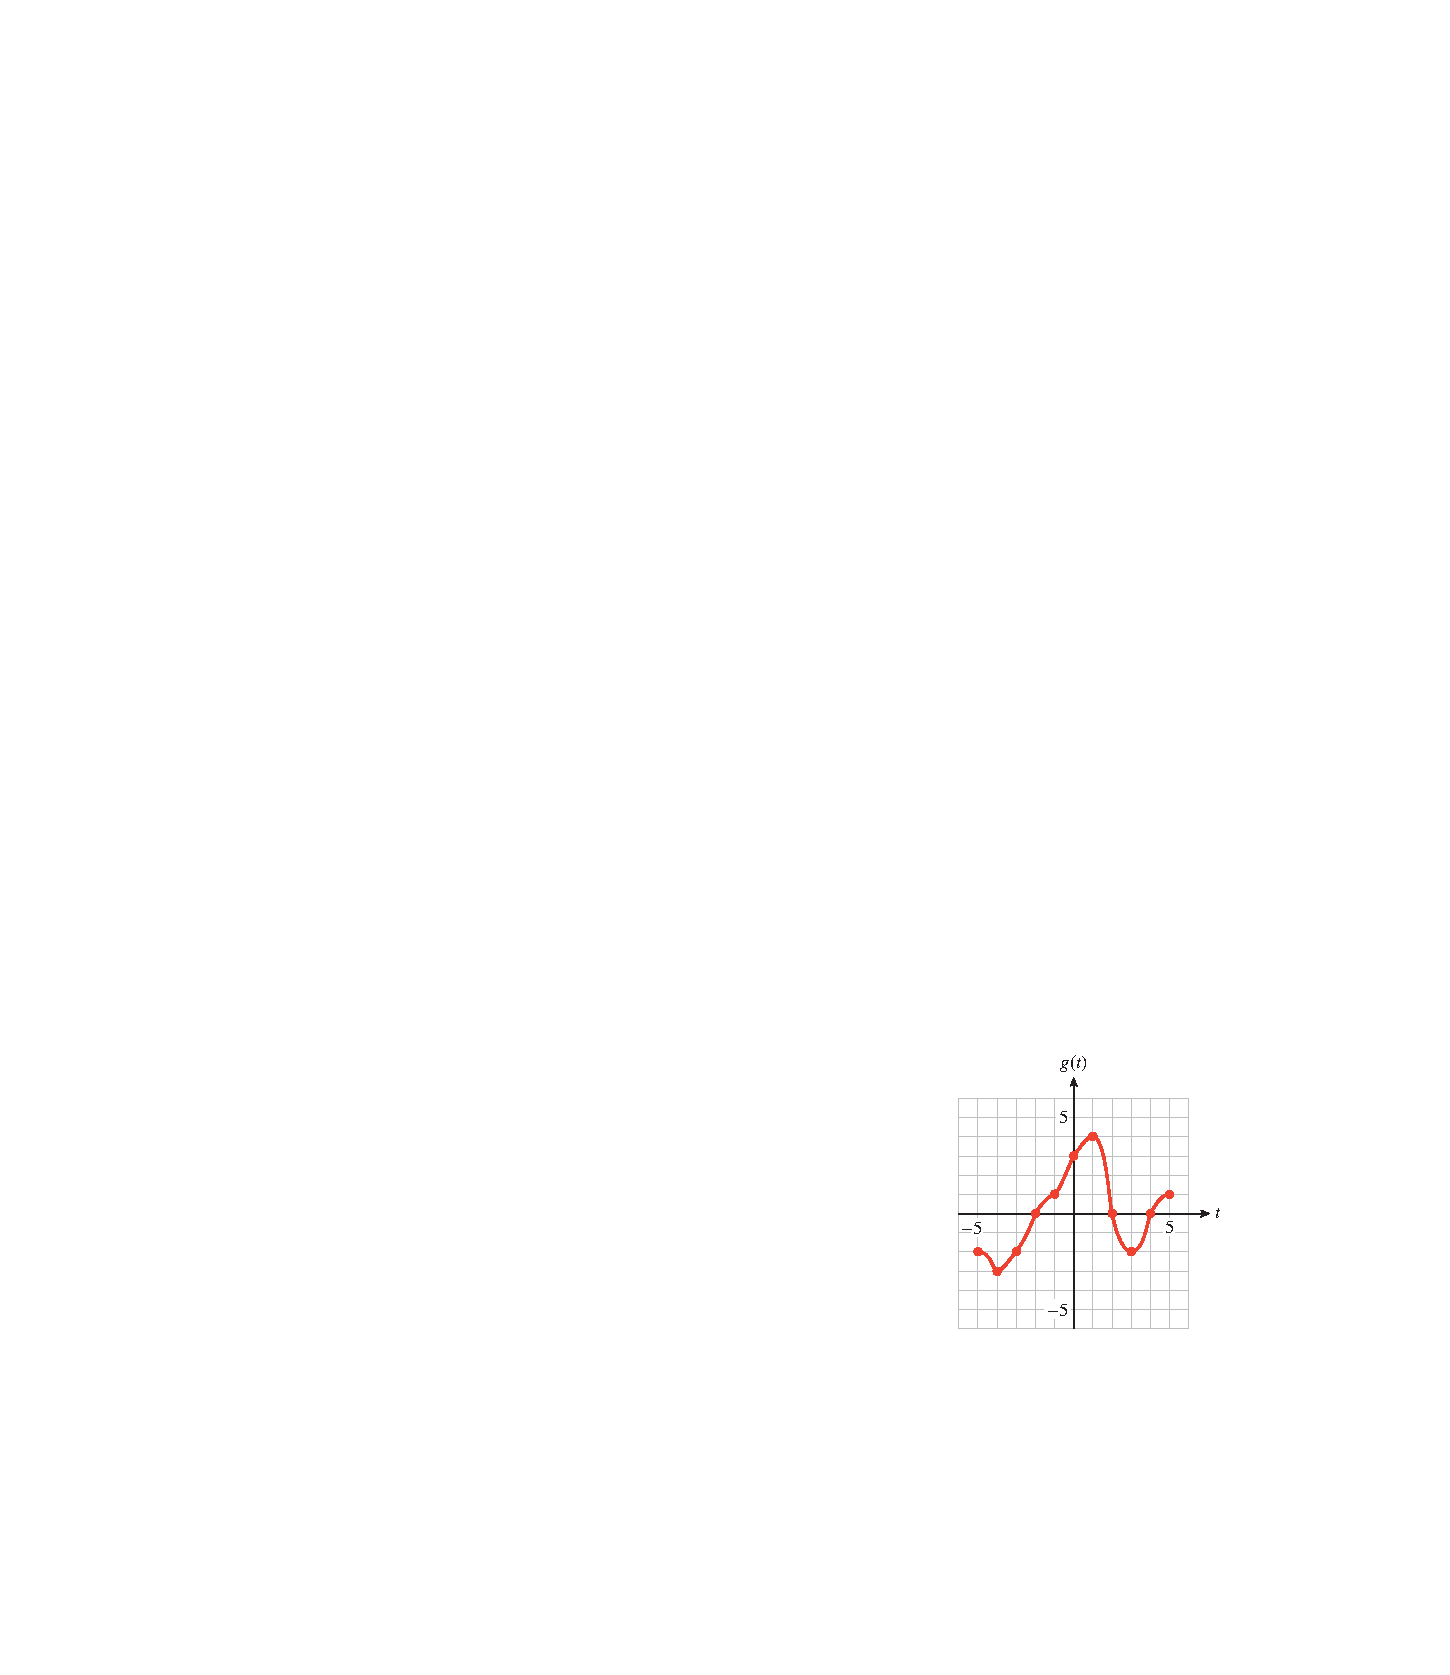
\includegraphics[width=0.60\textwidth,]{images/fig-function.pdf}\caption{\label{fig-function}}
\end{figure}
\par\medskip\noindent%
\textbf{Solution.}\quad \leavevmode%
\begin{enumerate}[label=*\alph**]
\item\hypertarget{li-125}{}To find \(g(−2)\), we look for the point with \(t\)-coordinate \(−2\). The point \((−2, 0)\) lies on the graph of \(g\), so \(g(−2) = 0\). Similarly, the point \((5, 1)\) lies on the graph, so \(g(5) = 1\).\item\hypertarget{li-126}{}We look for points on the graph with \(y\)-coordinate \(−2\). Because the points \((−5, −2)\), \((−3, −2)\), and \((3, −2)\) lie on the graph, we know that \(g(−5) = −2\), \(g(−3) = −2\), and \(g(3) = −2\). Thus, the \(t\)-values we want are \(−5\), \(−3\), and \(3\).\item\hypertarget{li-127}{}The highest point on the graph is \((1, 4)\), so the largest \(y\)-value is \(4\). Thus, the maximum value of \(g(t)\) is \(4\), and it occurs when \(t = 1\).\item\hypertarget{li-128}{}A graph is increasing if the \(y\)-values get larger as we read from left to right. The graph of \(g\) is increasing for \(t\)-values between \(−4\) and \(1\), and between \(3\) and \(5\). Thus, \(g\) is increasing on the intervals \((−4, 1)\) and \((3, 5)\).\end{enumerate}
\end{example}
\begin{exercise}\label{exercise-function-graph}

    Refer to the graph of the function \(g\) shown in \hyperref[fig-function]{Figure~\ref{fig-function}} in \hyperref[example-function-graph]{Example~\ref{example-function-graph}}.
    \leavevmode%
\begin{enumerate}[label=*\alph**]
\item\hypertarget{li-129}{}Find \(g(0)\).\item\hypertarget{li-130}{}For what value(s) of \(t\) is \(g(t) = 0\)?\item\hypertarget{li-131}{}What is the smallest, or minimum, value of \(g(t)\)? For what value of \(t\) does the function take on its minimum value?\item\hypertarget{li-132}{}On what intervals is \(g\) decreasing?\end{enumerate}
\end{exercise}
\begin{remark}[
\includegraphics[width=0.8\textwidth,]{images/icon-GC.pdf}Finding Coordinates with a Graphing Calculator]\label{remark-5}
We can use the 
\includegraphics[width=0.12\textwidth,]{images/icon-trace.pdf} feature of the calculator to find the coordinates of points on a graph. For example, graph the equation \(y = −2.6x − 5.4\) in the window%
\leavevmode%
\begin{table}
\centering
\begin{tabular}{lll}
Xmin\(=-5\)&&Xmax\(=4.4\)\tabularnewline[0pt]
Ymin\(=-20\)&&Ymax\(=15\)
\end{tabular}
\end{table}
\leavevmode%
\begin{figure}
\centering
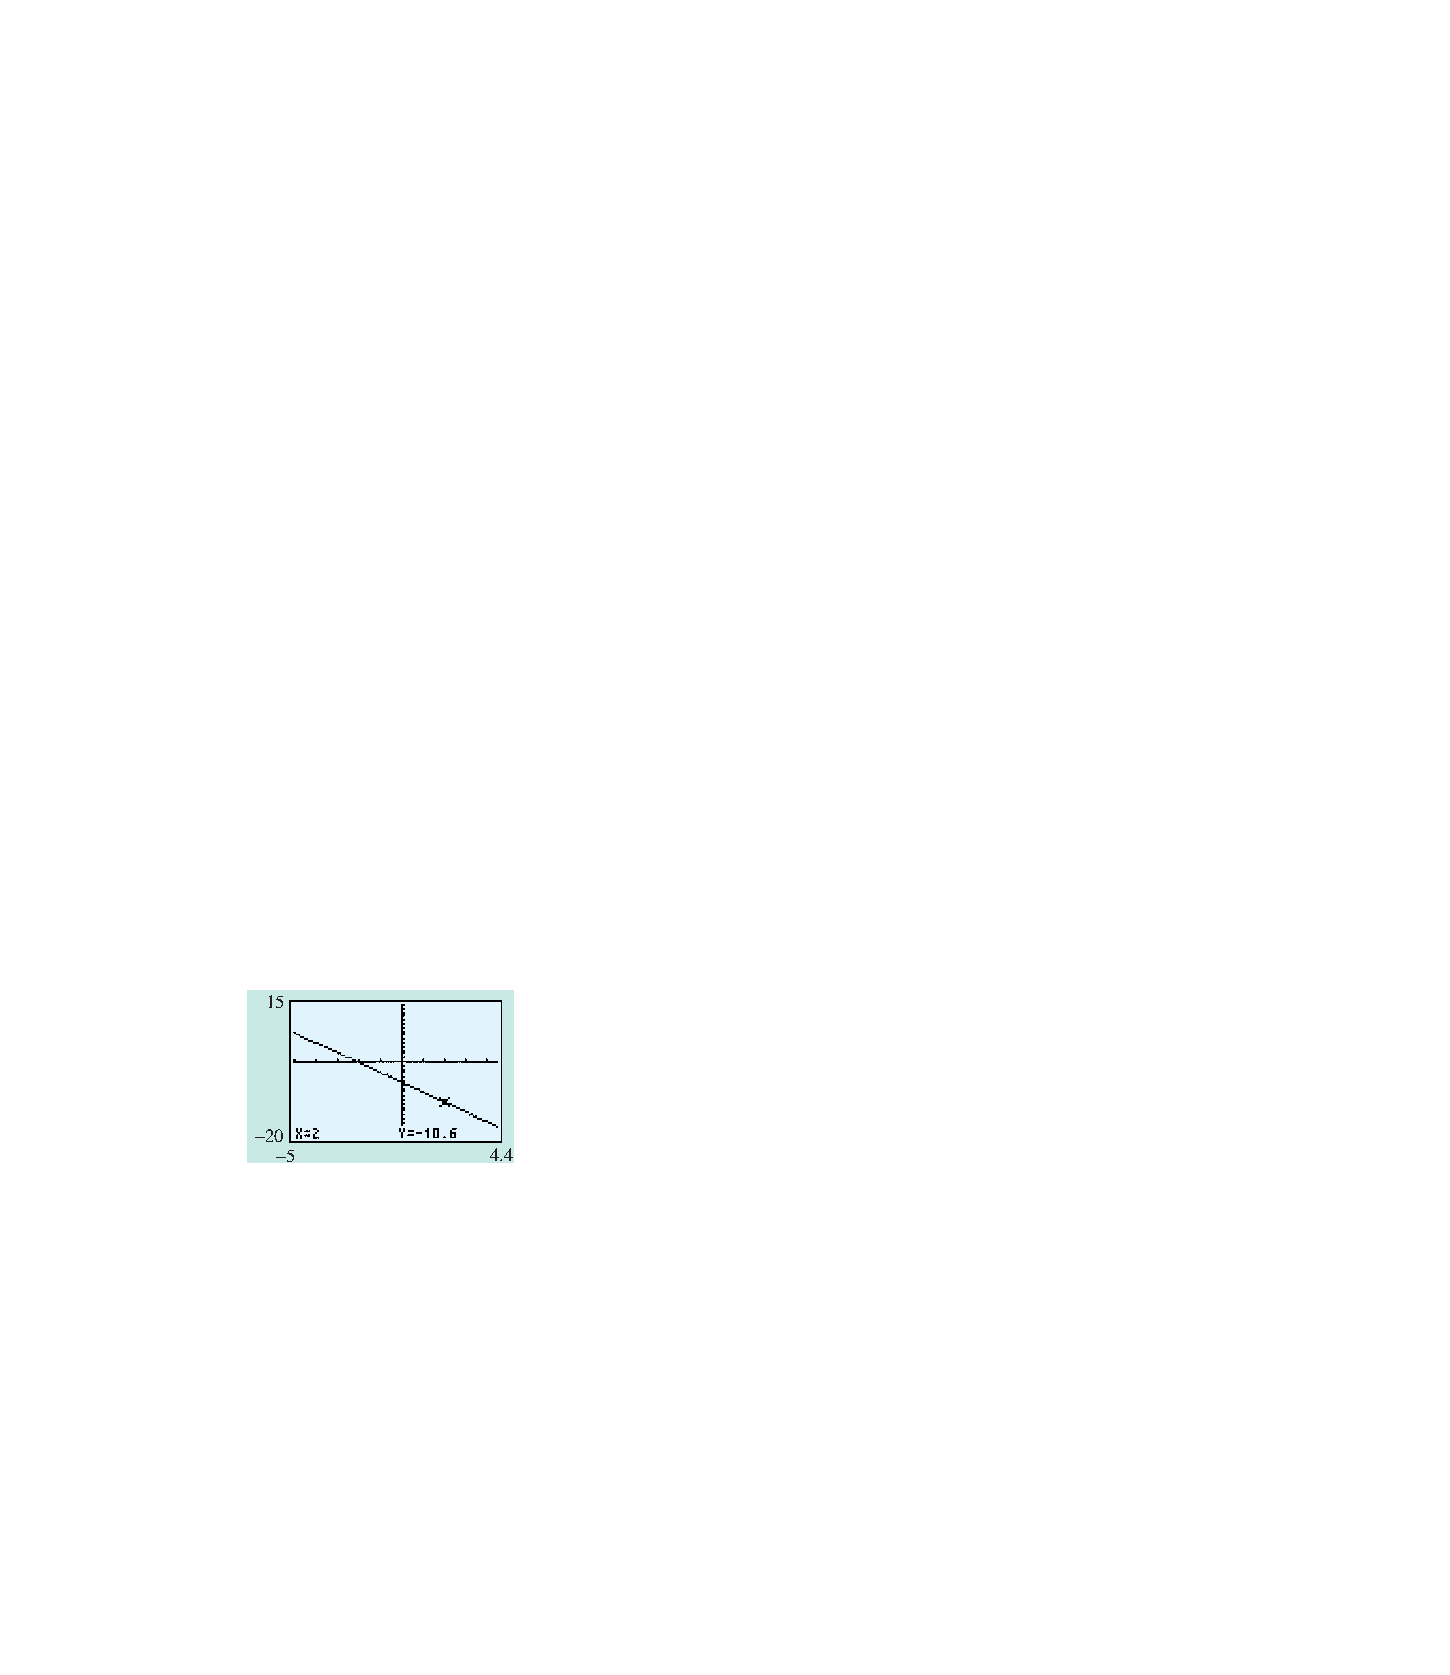
\includegraphics[width=0.60\textwidth,]{images/fig-GC-trace.pdf}\caption{\label{fig-GC-trace}}
\end{figure}
\par
Press 
\includegraphics[width=0.12\textwidth,]{images/icon-trace.pdf}, and a “bug” begins flashing on the display. The coordinates of the bug appear at the bottom of the display, as shown in \hyperref[fig-GC-trace]{Figure~\ref{fig-GC-trace}}. Use the left and right arrows to move the bug along the graph. You can check that the coordinates of the point \((2, −10.6)\) do satisfy the equation \(y = −2.6x − 5.4\).%
\par
The points identified by the Trace bug depend on the window settings and on the type of calculator. If we want to find the \(y\)-coordinate for a particular \(x\)-value, we enter the \(x\)-coordinate of the desired point and press 
\includegraphics[width=0.11\textwidth,]{images/icon-enter.pdf}.%
\end{remark}
\typeout{************************************************}
\typeout{Subsection 1.3.2 Constructing the Graph of a Function}
\typeout{************************************************}
\subsection[Constructing the Graph of a Function]{Constructing the Graph of a Function}\label{subsection-14}
Although some functions are defined by their graphs, we can also construct graphs for
functions described by tables or equations. We make these graphs the same way we graph
equations in two variables: by plotting points whose coordinates satisfy the equation.%
\begin{example}[]\label{example-graph-square-root}
Graph the function \(f(x) = \sqrt{x + 4}\).%
\par\medskip\noindent%
\textbf{Solution.}\quad Choose several convenient values for \(x\) and evaluate the function to find the corresponding \(f(x)\)-values. For this function we cannot choose \(x\)-values less than \(−4\), because the square root of a negative number is not a real number. 
    \begin{equation*}f(\alert{−4}) =\sqrt{\alert{−4} + 4}=\sqrt{0}= 0\end{equation*}
    \begin{equation*}f(\alert{−3}) =\sqrt{\alert{−3} + 4}=\sqrt{1}= 1\end{equation*}
    \begin{equation*}f(\alert{0}) =\sqrt{\alert{0} + 4}=\sqrt{4}=2\end{equation*}
    \begin{equation*}f(\alert{2}) =\sqrt{\alert{2} + 4}=\sqrt{6}\approx 2.45\end{equation*}
    \begin{equation*}f(\alert{5}) =\sqrt{\alert{5} + 4}=\sqrt{9}=3\end{equation*}
    The results are shown in the table.%
\leavevmode%
\begin{figure}
\centering
\pushValignCaptionBottom[b]{minipage}{.50\textwidth}{%
\centering% horizontal alignment 
\begin{tabular}{AcAcA}\hrulethick
\(x\)%
&\(f(x)\)%
\tabularnewline\hrulethin
\(-4\)&\(0\)\tabularnewline\hrulethin
\(-3\)&\(1\)\tabularnewline\hrulethin
\(0\)&\(2\)\tabularnewline\hrulethin
\(2\)&\(\sqrt{6}\)\tabularnewline\hrulethin
\(5\)&\(3\)\tabularnewline\hrulethin
\end{tabular}
}% end body 
{}% caption 
\pushValignCaptionBottom[b]{minipage}{.50\textwidth}{%
\centering% horizontal alignment 
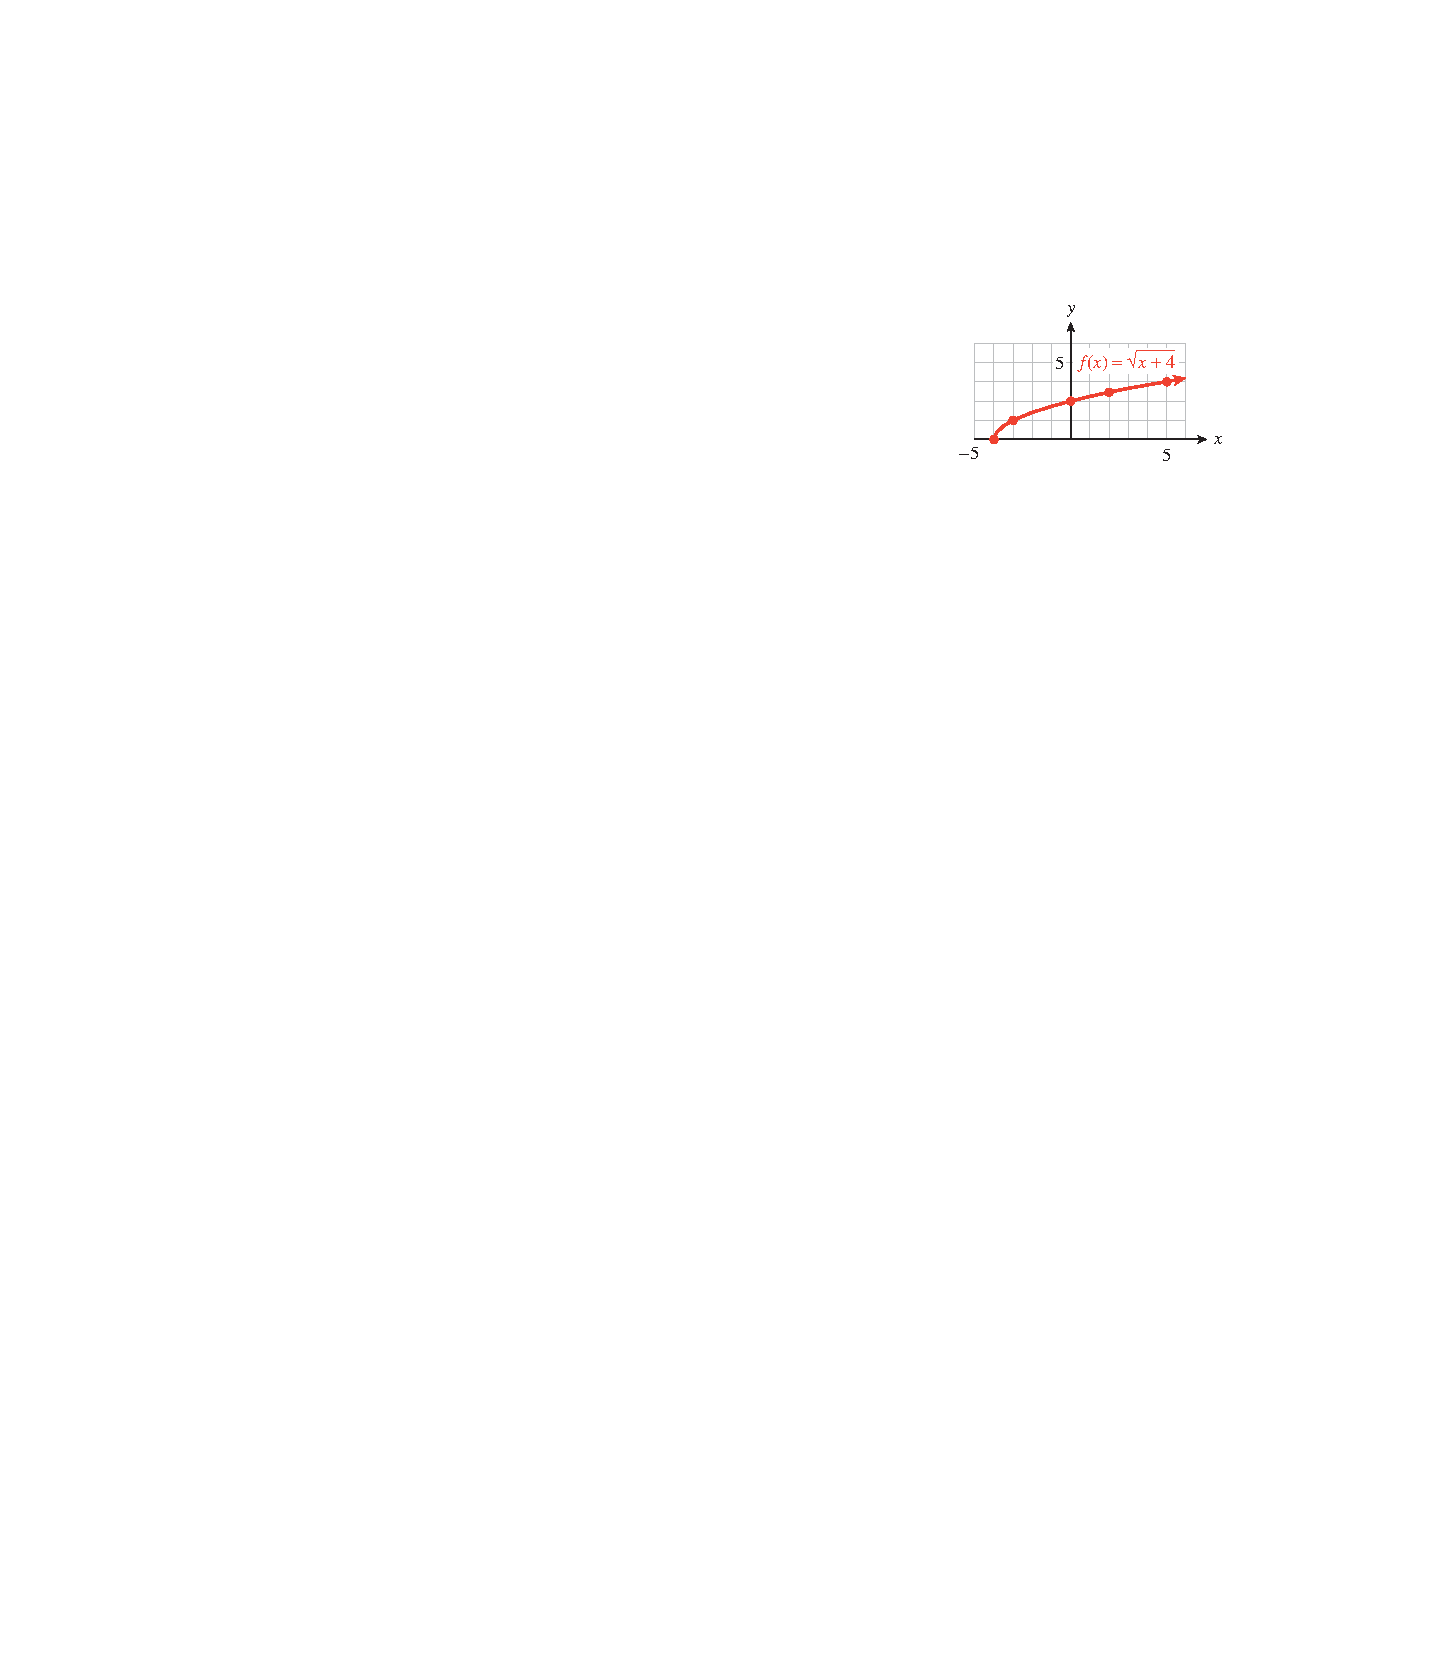
\includegraphics[width=\textwidth,]{images/fig-sq-root.pdf}}% end body 
{\captionof{figure}{\label{fig-sq-root}}
}% caption 
\popValignCaptionBottom
\end{figure}
\end{example}
\begin{remark}[
\includegraphics[width=0.8\textwidth,]{images/icon-GC.pdf}Using a Calculator to Graph a Function]\label{remark-6}
We can also use a graphing calculator to obtain a table and graph for the function in \hyperref[example-graph-square-root]{Example~\ref{example-graph-square-root}}. We graph a function just as we graphed an equation. For this function, we enter \begin{equation*}Y_1 = \sqrt{~^~}(X+4)\end{equation*}
    and press 
\includegraphics[width=0.12\textwidth,]{images/icon-zoom.pdf}\(6\) for the standard window. (See {$\langle\langle$appendix-b$\rangle\rangle$}  for details.) The calculator’s graph is shown in \hyperref[fig-GC-sq-root]{Figure~\ref{fig-GC-sq-root}}.%
\leavevmode%
\begin{figure}
\centering
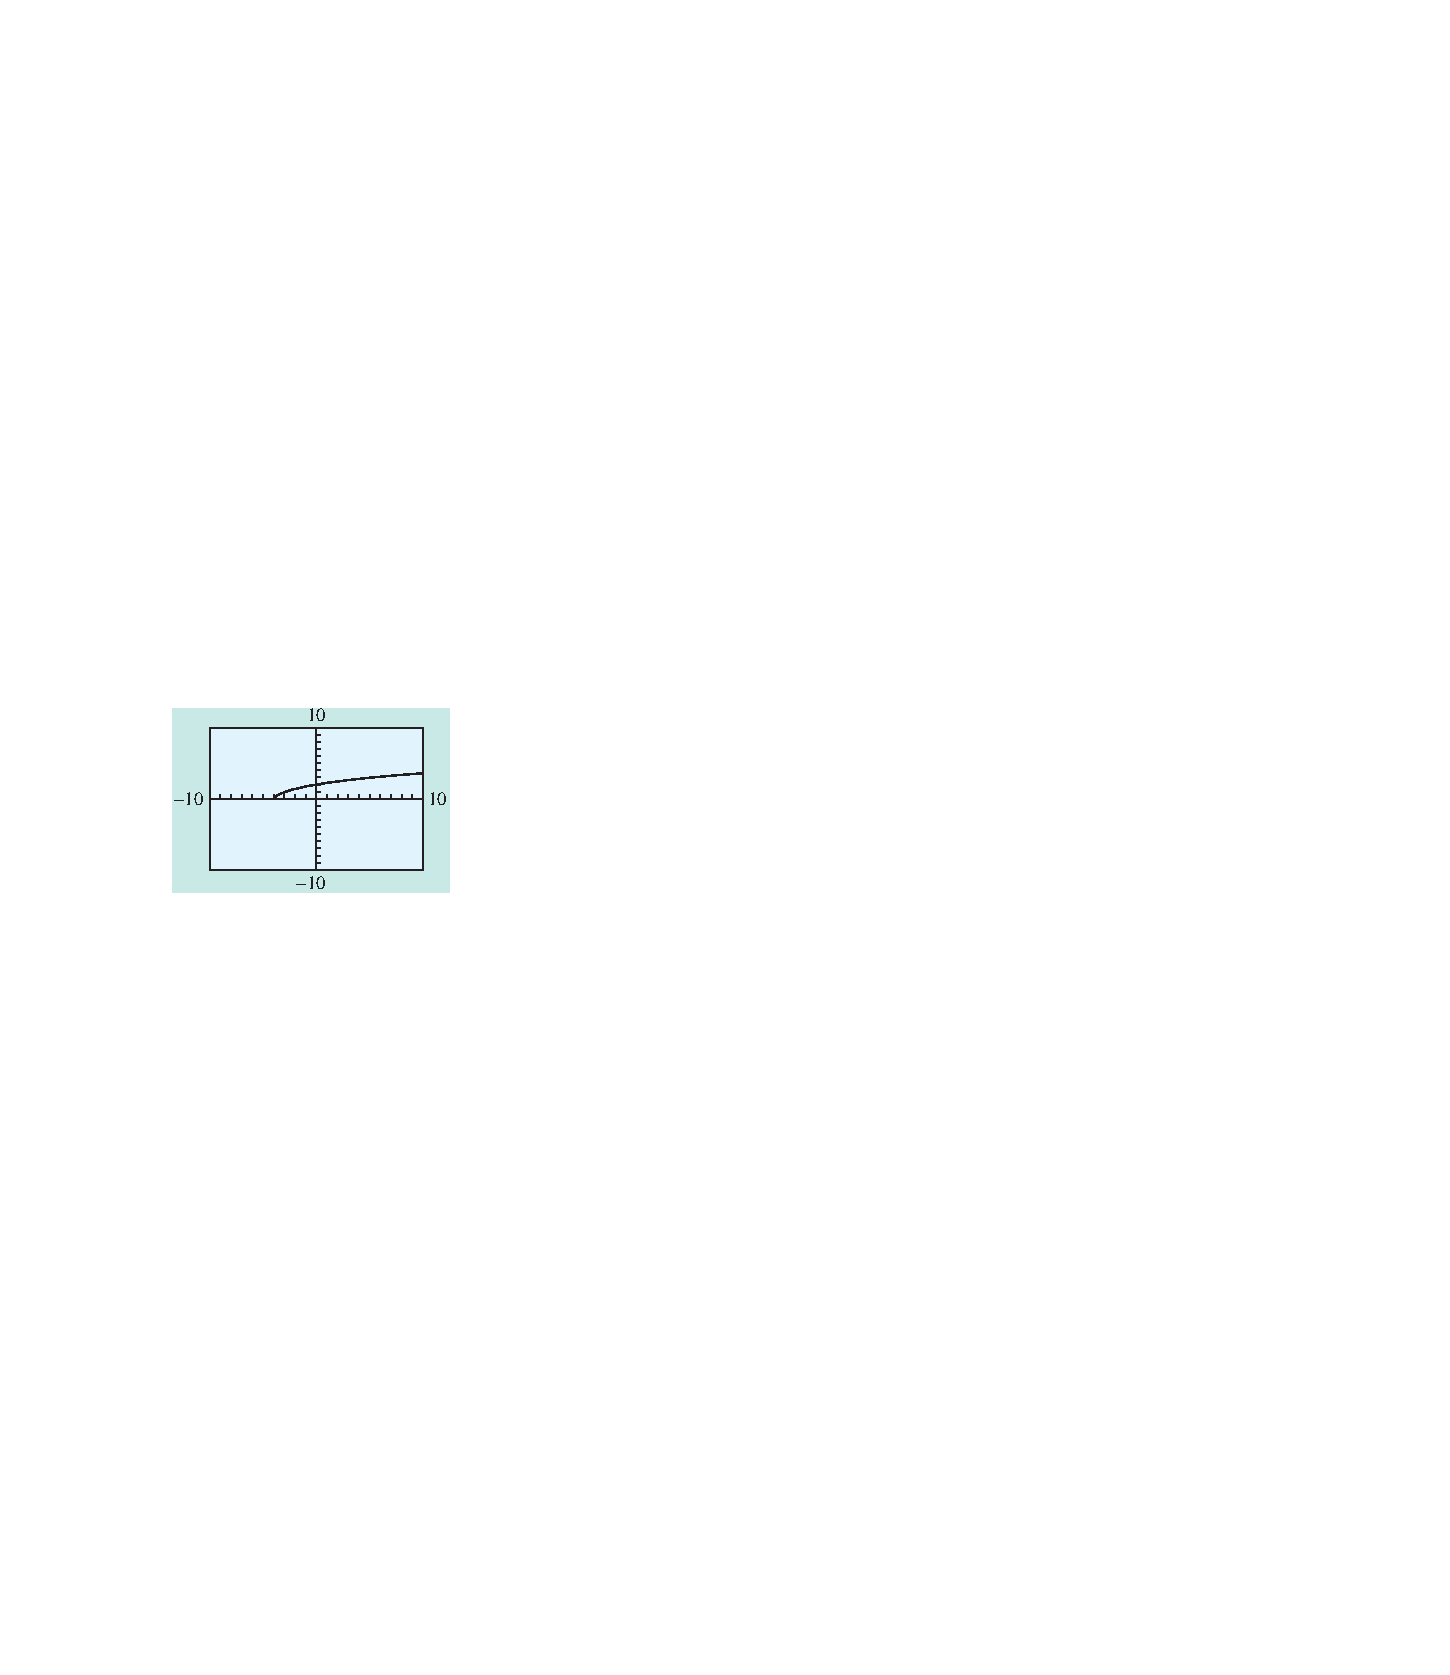
\includegraphics[width=0.50\textwidth,]{images/fig-GC-sq-root.pdf}\caption{\label{fig-GC-sq-root}}
\end{figure}
\end{remark}
\begin{exercise}\label{exercise-cubic-graph}
\begin{equation*}f(x) = x^3 − 2\end{equation*}\leavevmode%
\begin{enumerate}[label=*\alph**]
\item\hypertarget{li-133}{}Complete the table of values and sketch a graph of the function.
    \leavevmode%
\begin{table}
\centering
\begin{tabular}{AcAcAcAcAcAcAcAcA}\hrulethick
\(x\)&\(-2\)&\(-1\)&\(-\frac{1}{2}\)&\(0\)&\(\frac{1}{2}\)&\(1\)&\(2\)\tabularnewline\hrulethin
\(f(x)\)&%
&%
&%
&%
&%
&%
&%
\tabularnewline\hrulethin
\end{tabular}
\end{table}
\item\hypertarget{li-134}{}Use your calculator to make a table of values and graph the function.\end{enumerate}
\end{exercise}
\typeout{************************************************}
\typeout{Subsection 1.3.3 The Vertical Line Test}
\typeout{************************************************}
\subsection[The Vertical Line Test]{The Vertical Line Test}\label{subsection-15}
In a function, two different outputs cannot be related to the same input. This restriction means that two different ordered pairs cannot have the same first coordinate. What does it mean for the graph of the function?%
\par
Consider the graph shown in \hyperref[fig-vertical-line-test]{Figure~\ref{fig-vertical-line-test}}a. Every vertical line intersects the graph in at most one point, so there is only one point on the graph for each \(x\)-value. This graph represents a function. In \hyperref[fig-vertical-line-test]{Figure~\ref{fig-vertical-line-test}}b, however, the line \(x = 2\) intersects the graph at two points, \((2, 1)\) and \((2, 4)\). Two different \(y\)-values, \(1\) and \(4\), are related to the same \(x\)-value, \(2\). This graph cannot be the graph of a function.%
\leavevmode%
\begin{figure}
\centering
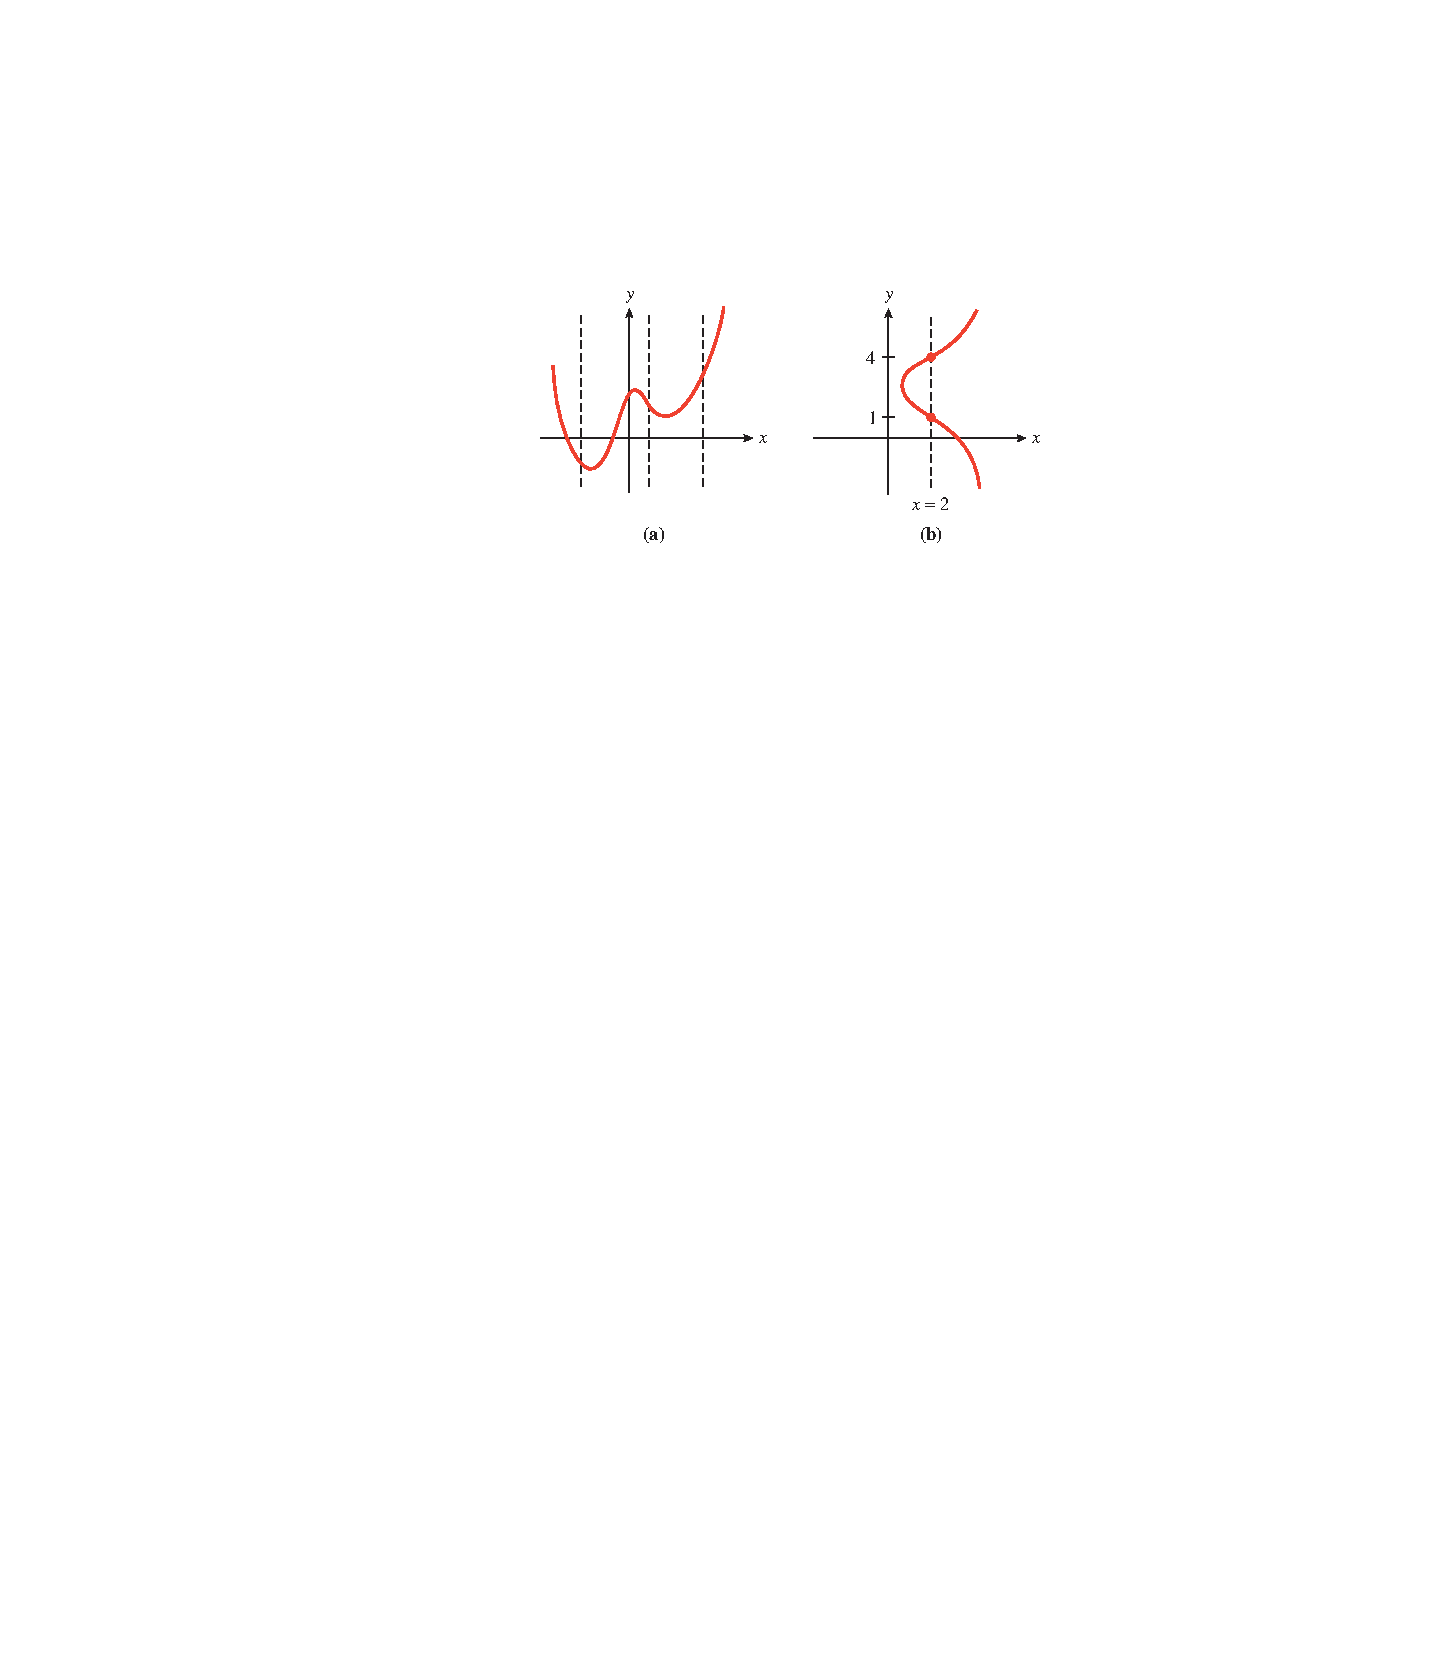
\includegraphics[width=0.90\textwidth,]{images/fig-vertical-line-test.pdf}\caption{\label{fig-vertical-line-test}}
\end{figure}
\par
We summarize these observations as follows.%
\typeout{************************************************}
\typeout{Paragraphs  The Vertical Line Test}
\typeout{************************************************}
\paragraph[The Vertical Line Test]{The Vertical Line Test}\label{paragraphs-9}
A graph represents a function if and only if every vertical line intersects the graph in
at most one point.%
\begin{example}[]\label{example-vertical-line-test}
Use the vertical line test to decide which of the graphs in \hyperref[fig-vertical-line-test2]{Figure~\ref{fig-vertical-line-test2}}  represent functions.%
\leavevmode%
\begin{figure}
\centering
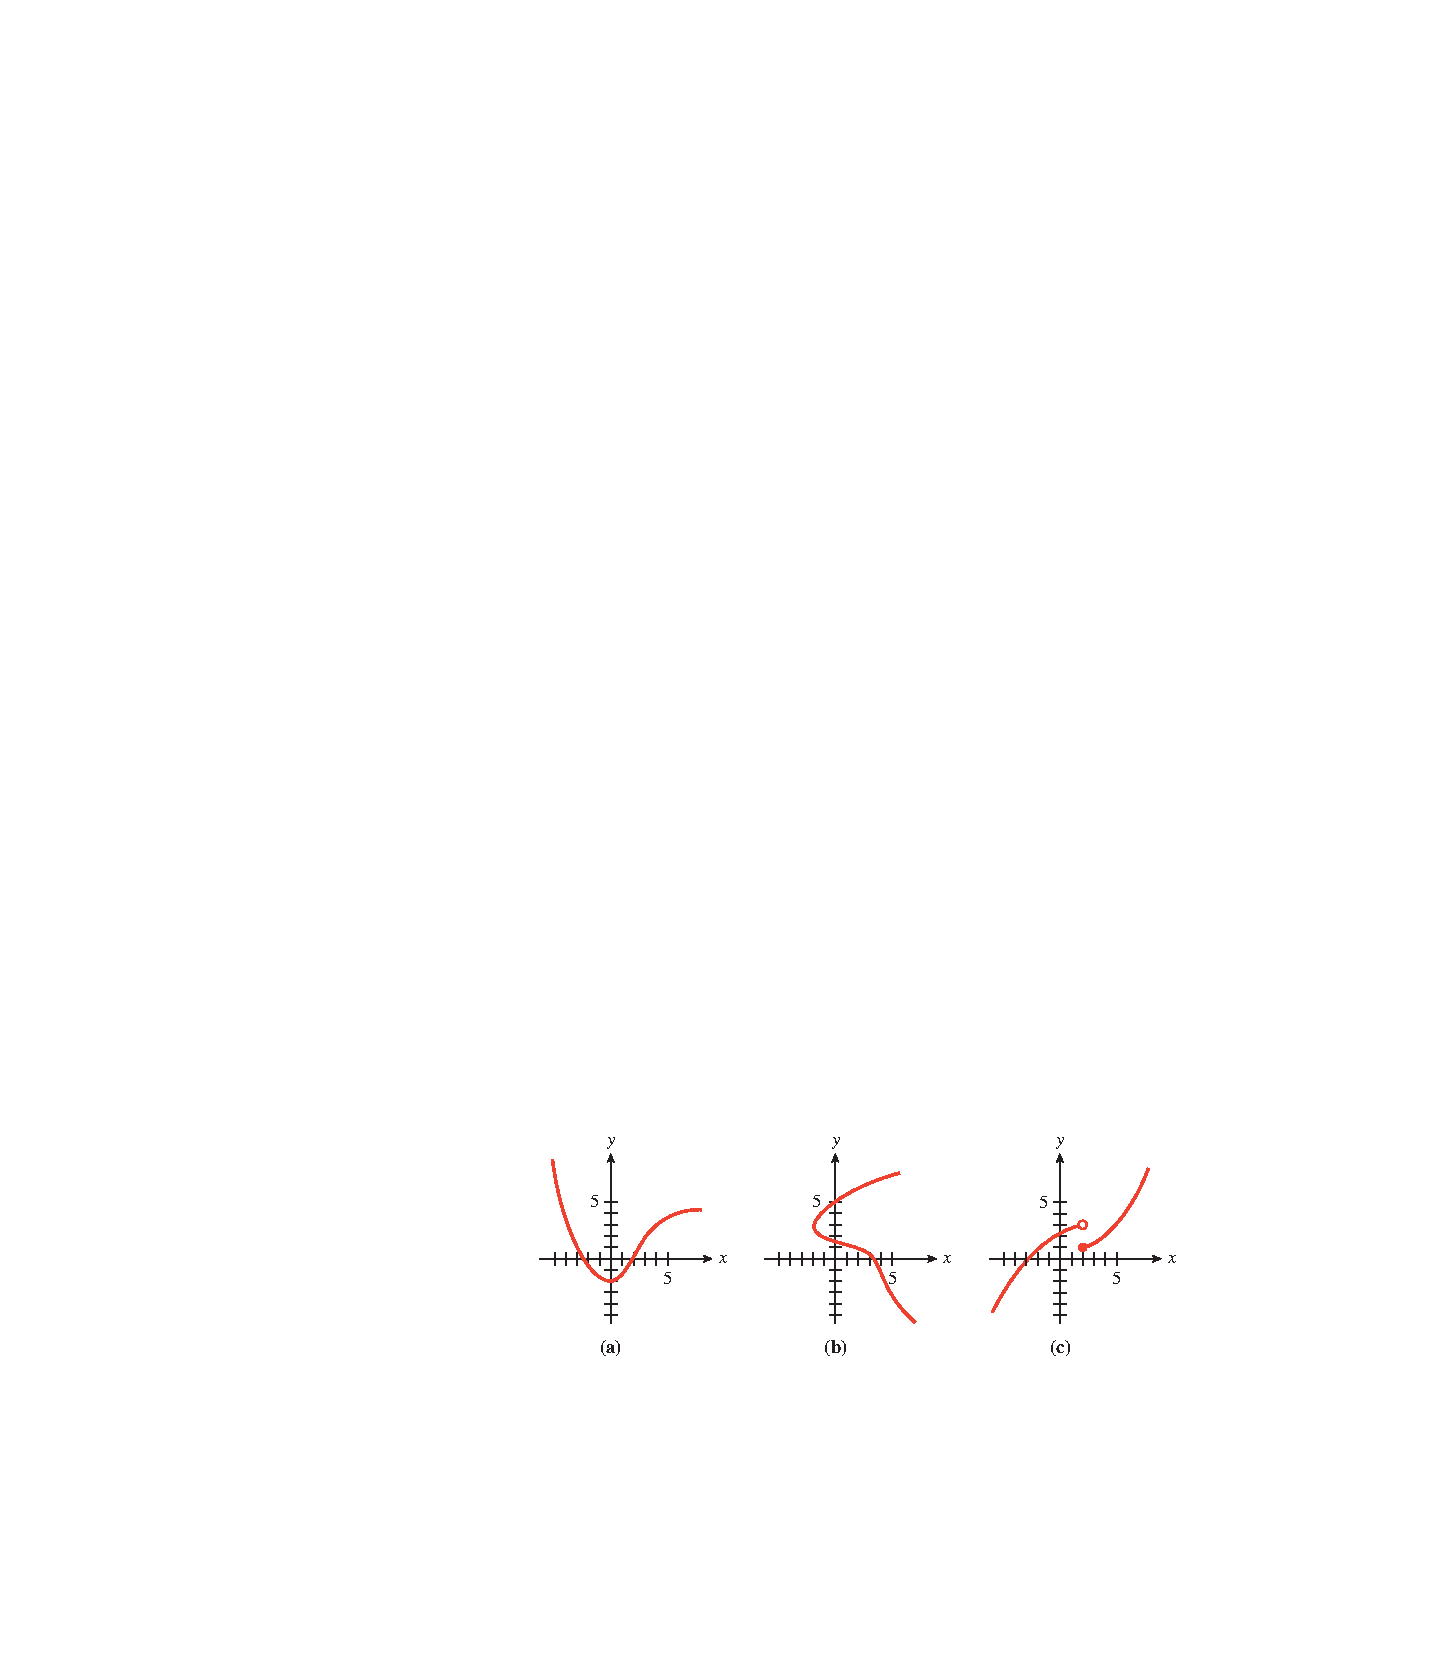
\includegraphics[width=0.90\textwidth,]{images/fig-vertical-line-test2.pdf}\caption{\label{fig-vertical-line-test2}}
\end{figure}
\par\medskip\noindent%
\textbf{Solution.}\quad 
    Graph (a) represents a function, because it passes the vertical line test. Graph (b) is not the graph of a function, because the vertical line at (for example) \(x = 1\) intersects the graph at two points. For graph (c), notice the break in the curve at \(x = 2\): The solid dot at \((2, 1)\) is the only point on the graph with \(x = 2\); the open circle at \((2, 3)\) indicates that \((2, 3)\) is not a point on the graph. Thus, graph (c) is a function, with \(f(2) = 1\).
\end{example}
\begin{exercise}\label{example-vertical-line-test3}
Use the vertical line test to determine which of the graphs in \hyperref[fig-vertical-line-test3]{Figure~\ref{fig-vertical-line-test3}} represent functions.
    \leavevmode%
\begin{figure}
\centering
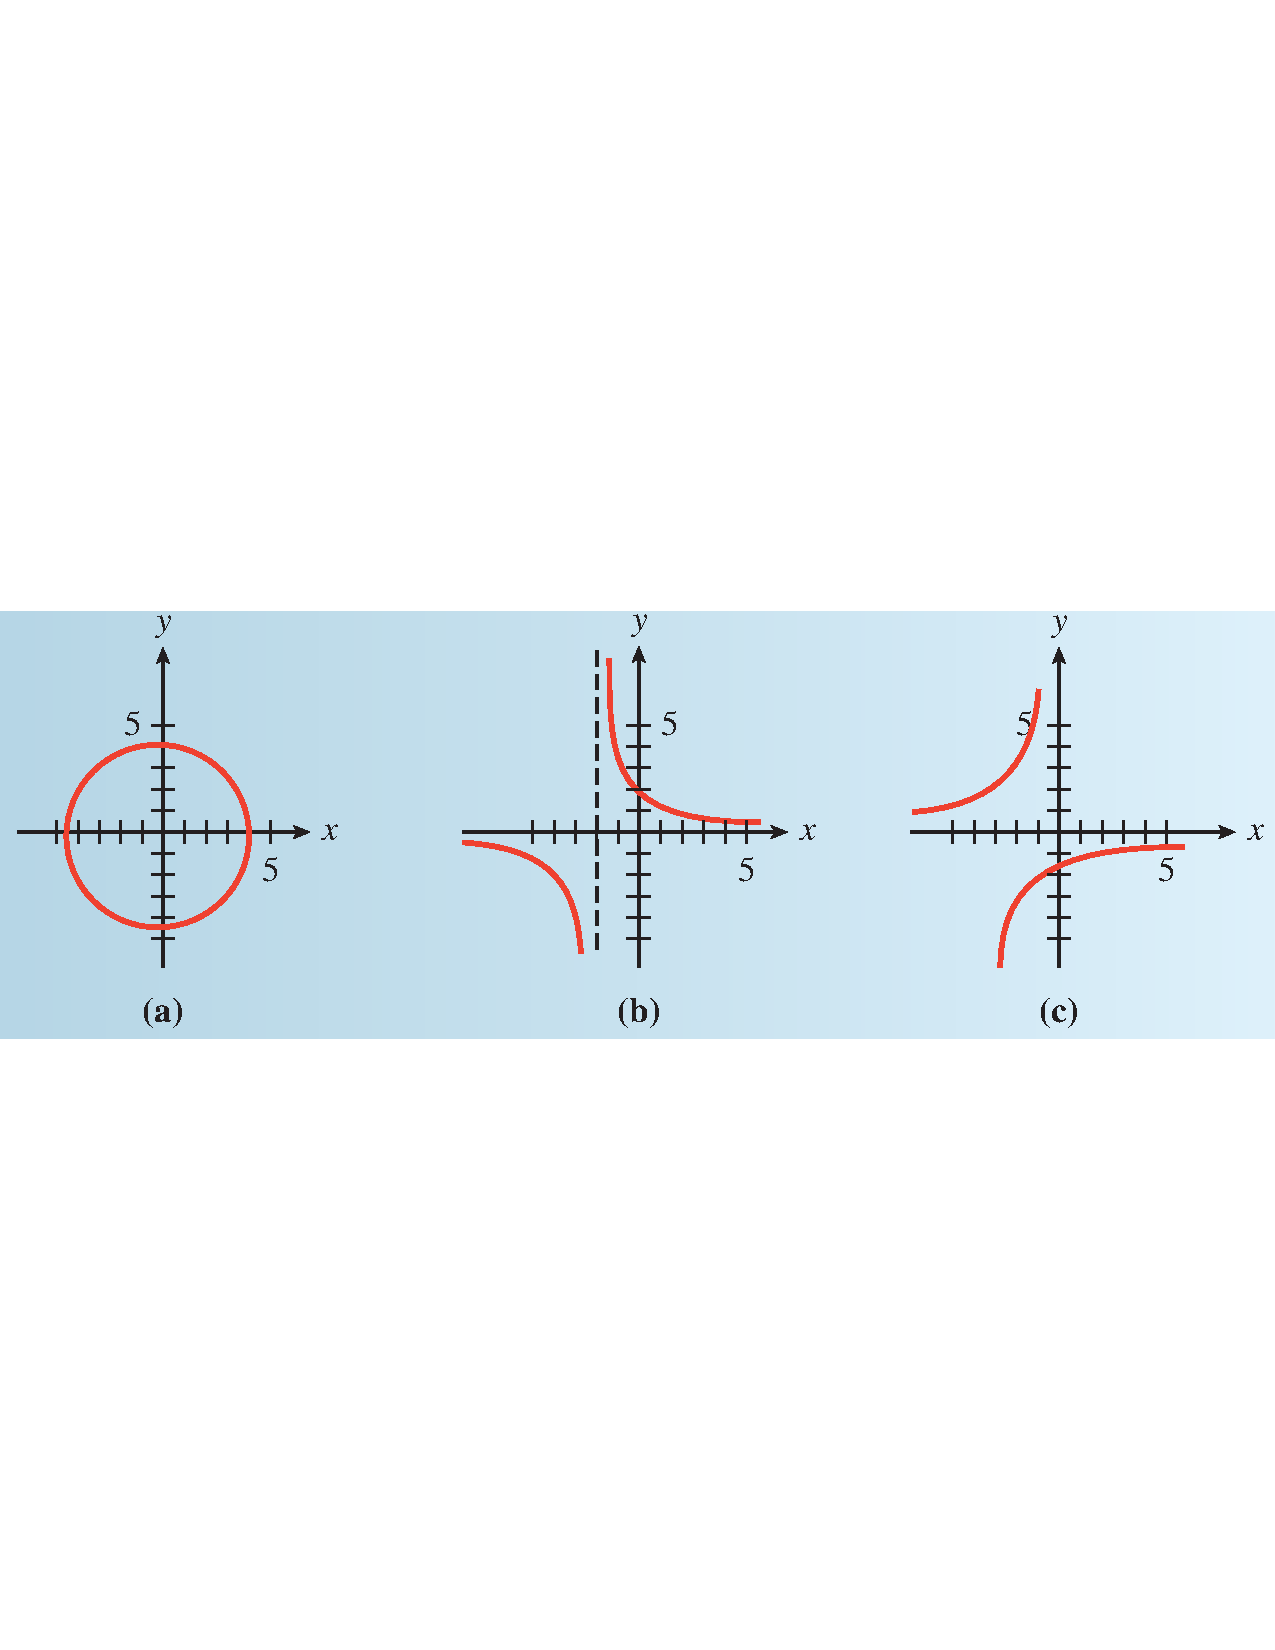
\includegraphics[width=0.100\textwidth,]{images/fig-vertical-line-test3.pdf}\caption{\label{fig-vertical-line-test3}}
\end{figure}
\end{exercise}
\typeout{************************************************}
\typeout{Subsection 1.3.4 Graphical Solution of Equations and Inequalities}
\typeout{************************************************}
\subsection[Graphical Solution of Equations and Inequalities]{Graphical Solution of Equations and Inequalities}\label{subsection-16}
The graph of an equation in two variables is just a picture of its solutions. When we read the coordinates of a point on the graph, we are reading a pair of \(x\)- and \(y\)-values that make the equation true. %
\leavevmode%
\begin{figure}
\centering
\pushValignCaptionBottom[b]{minipage}{.65\textwidth}{%
% horizontal alignment 
\parbox{\textwidth}{%
% horizontal alignment 
For example, the point \((2, 7)\) lies on the graph of \(y = 2x + 3\) shown in \hyperref[fig-function-graph]{Figure~\ref{fig-function-graph}} , so we know that the ordered pair \((2, 7)\) is a solution of the equation \(y = 2x + 3\). You can verify algebraically that \(x = \alert{2}\) and \(y = \alert{7}\) satisfy the equation: 
    \begin{equation*}\text{Does }~\alert{7} = 2 (\alert{2}) + 3\text{? Yes}\end{equation*}
    We can also say that \(x = 2\) is a solution of the one-variable equation \(2x + 3 = 7\). In fact, we can use the graph of \(y = 2x + 3\) to solve the equation \(2x + 3 = k\) for any value of \(k\). Thus, we can use graphs to find solutions to equations in one variable.%
}%
}% end body 
{}% caption 
\pushValignCaptionBottom[b]{minipage}{.35\textwidth}{%
\centering% horizontal alignment 
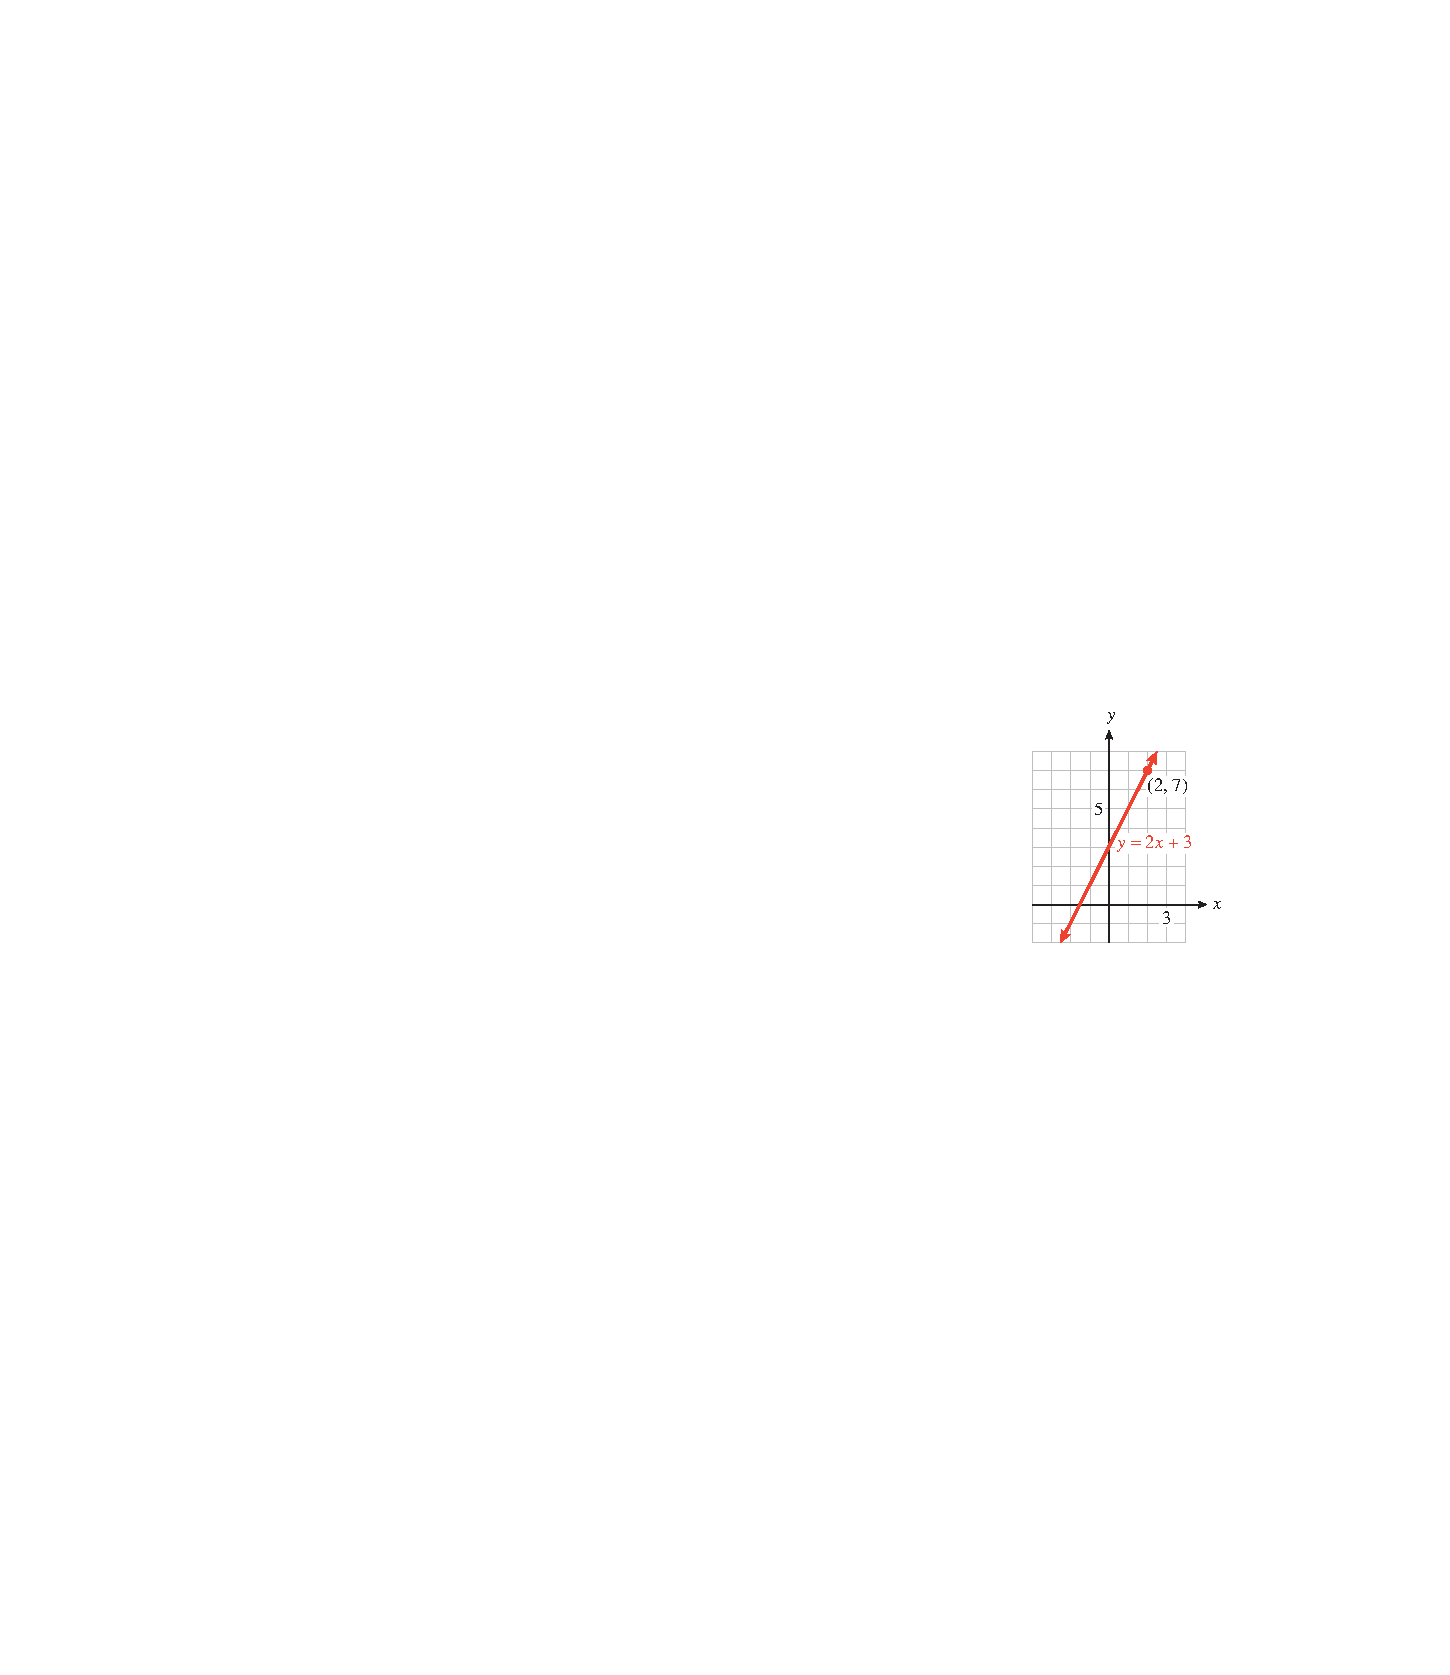
\includegraphics[width=\textwidth,]{images/fig-function-graph.pdf}}% end body 
{\captionof{figure}{\label{fig-function-graph}}
}% caption 
\popValignCaptionBottom
\end{figure}
\begin{example}[]\label{example-graph-to-solve}
Use the graph of \(y = 285 − 15x\) to solve the equation \(150 = 285 − 15x\).%
\par\medskip\noindent%
\textbf{Solution.}\quad \leavevmode%
\begin{figure}
\centering
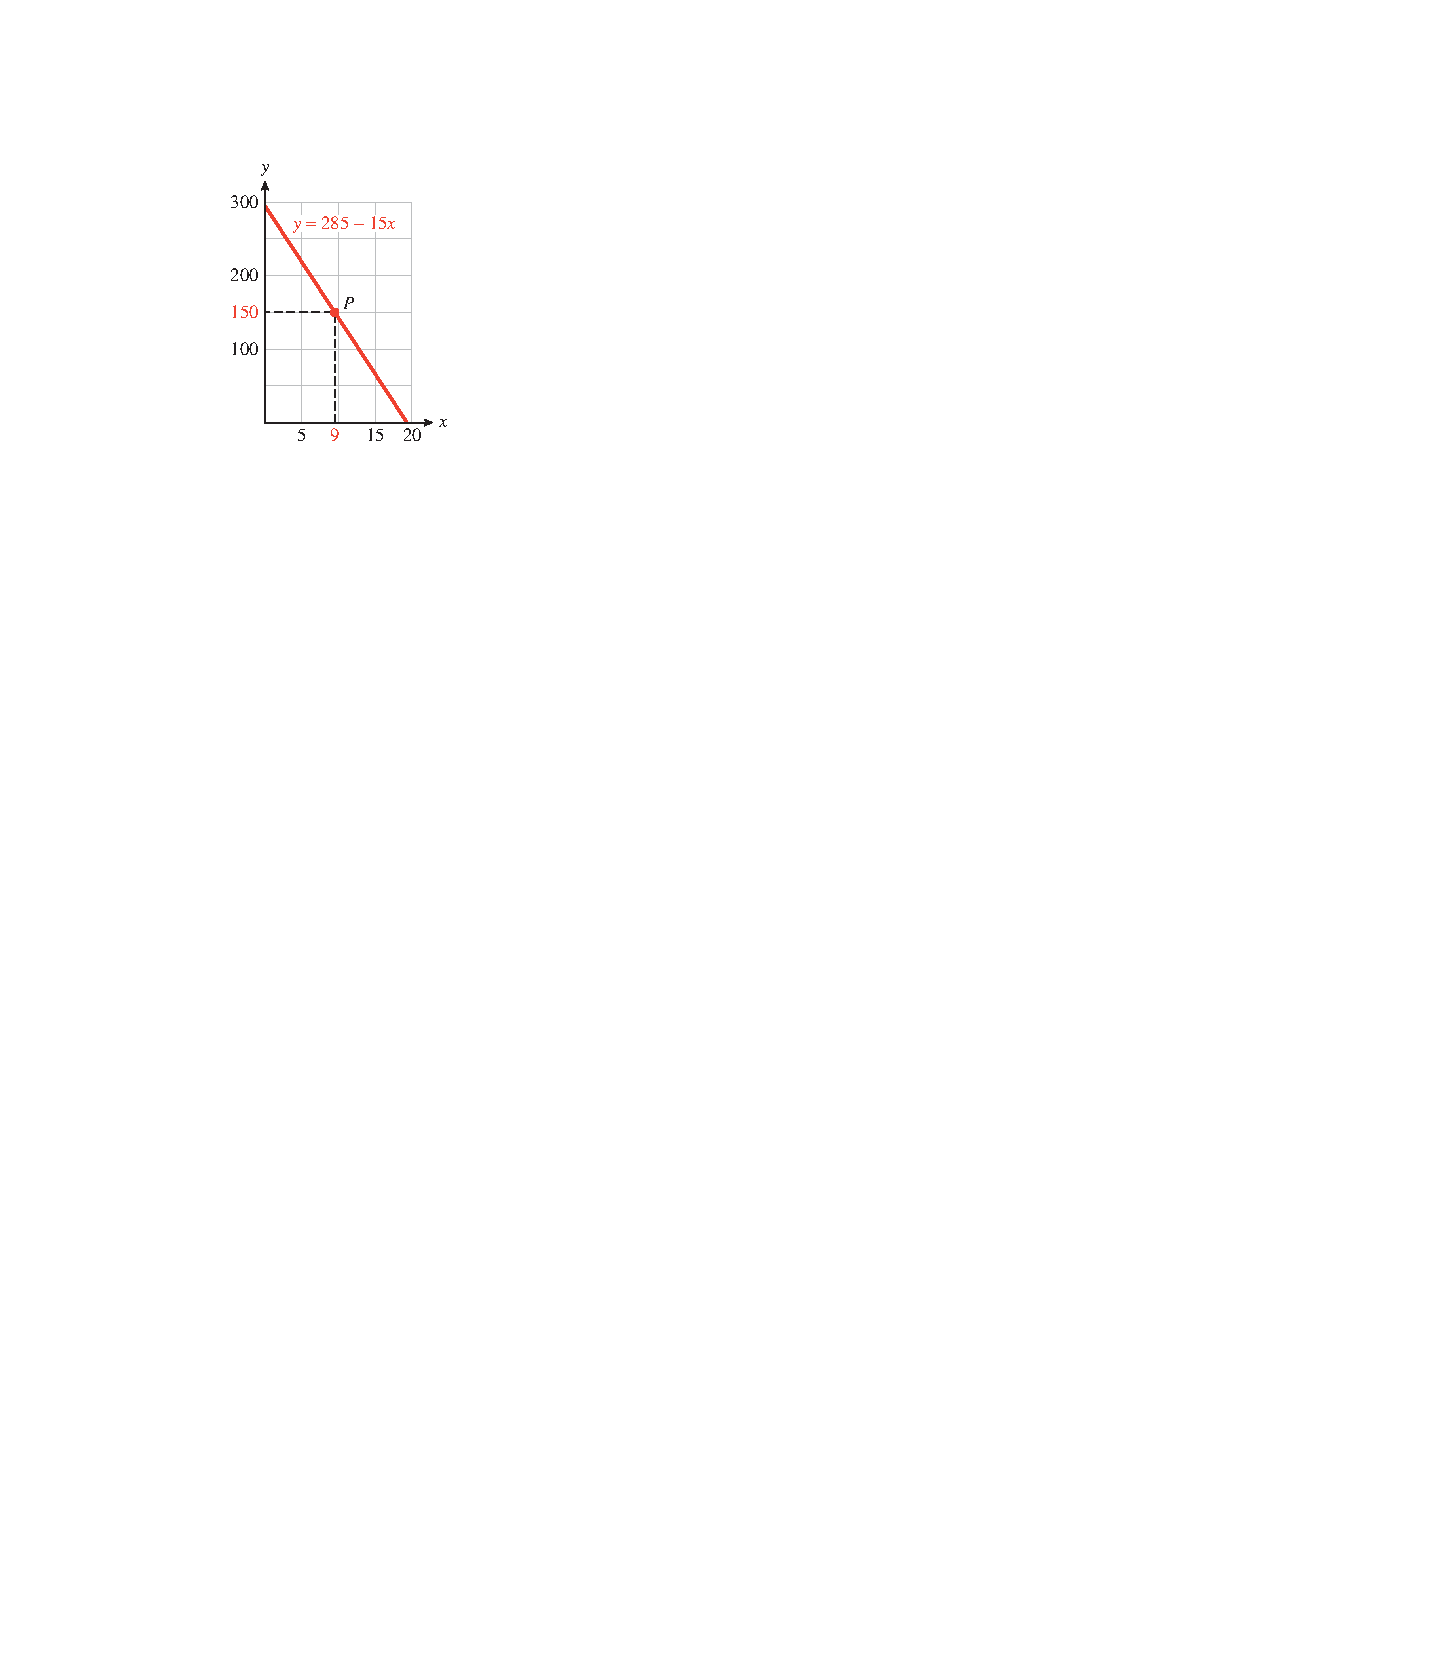
\includegraphics[width=0.50\textwidth,]{images/fig-graph-to-solve.pdf}\caption{\label{fig-graph-to-solve}}
\end{figure}
Begin by locating the point \(P\) on the graph for which \(y = 150\), as shown in \hyperref[fig-graph-to-solve]{Figure~\ref{fig-graph-to-solve}}. Now find the \(x\)-coordinate of point \(P\) by drawing an imaginary line from \(P\) straight down to the \(x\)-axis. The \(x\)-coordinate of \(P\) is \(x = 9\). Thus, \(P\) is the point \((9,150)\), and \(x = 9\) when \(y = 150\). The solution of the equation \(150 = 285 − 15x\) is \(x = 9\). You can verify the solution algebraically by substituting \(x = \alert{9}\) into the equation:%
\par
Does \(150 = 285 − 15(\alert{9})\)? %
\begin{equation*}285 − 15(\alert{9}) = 285 − 135 = 150. ~~\alert{Yes}\end{equation*}\end{example}
\par
The relationship between an equation and its graph is an important one. For the
previous example, make sure you understand that the following three statements are
equivalent:
%
\leavevmode%
\begin{enumerate}
\item\hypertarget{li-135}{}The point \((9, 150)\) lies on the graph of \(y = 285 − 15x\).\item\hypertarget{li-136}{}The ordered pair \((9, 150)\) is a solution of the equation \(y = 285 − 15x\).\item\hypertarget{li-137}{}\(x = 9\) is a solution of the equation \(150 = 285 − 15x\).\end{enumerate}
\begin{exercise}\label{exercise-graph-to-solve}
\leavevmode%
\begin{enumerate}[label=*\alph**]
\item\hypertarget{li-138}{}Use the graph of \(y = 30 − 8x\) shown in \hyperref[fig-graph-to-solve2]{Figure~\ref{fig-graph-to-solve2}} to solve the equation \begin{equation*}30 − 8x = 50\end{equation*}\item\hypertarget{li-139}{}Verify your solution algebraically.\end{enumerate}
\leavevmode%
\begin{figure}
\centering
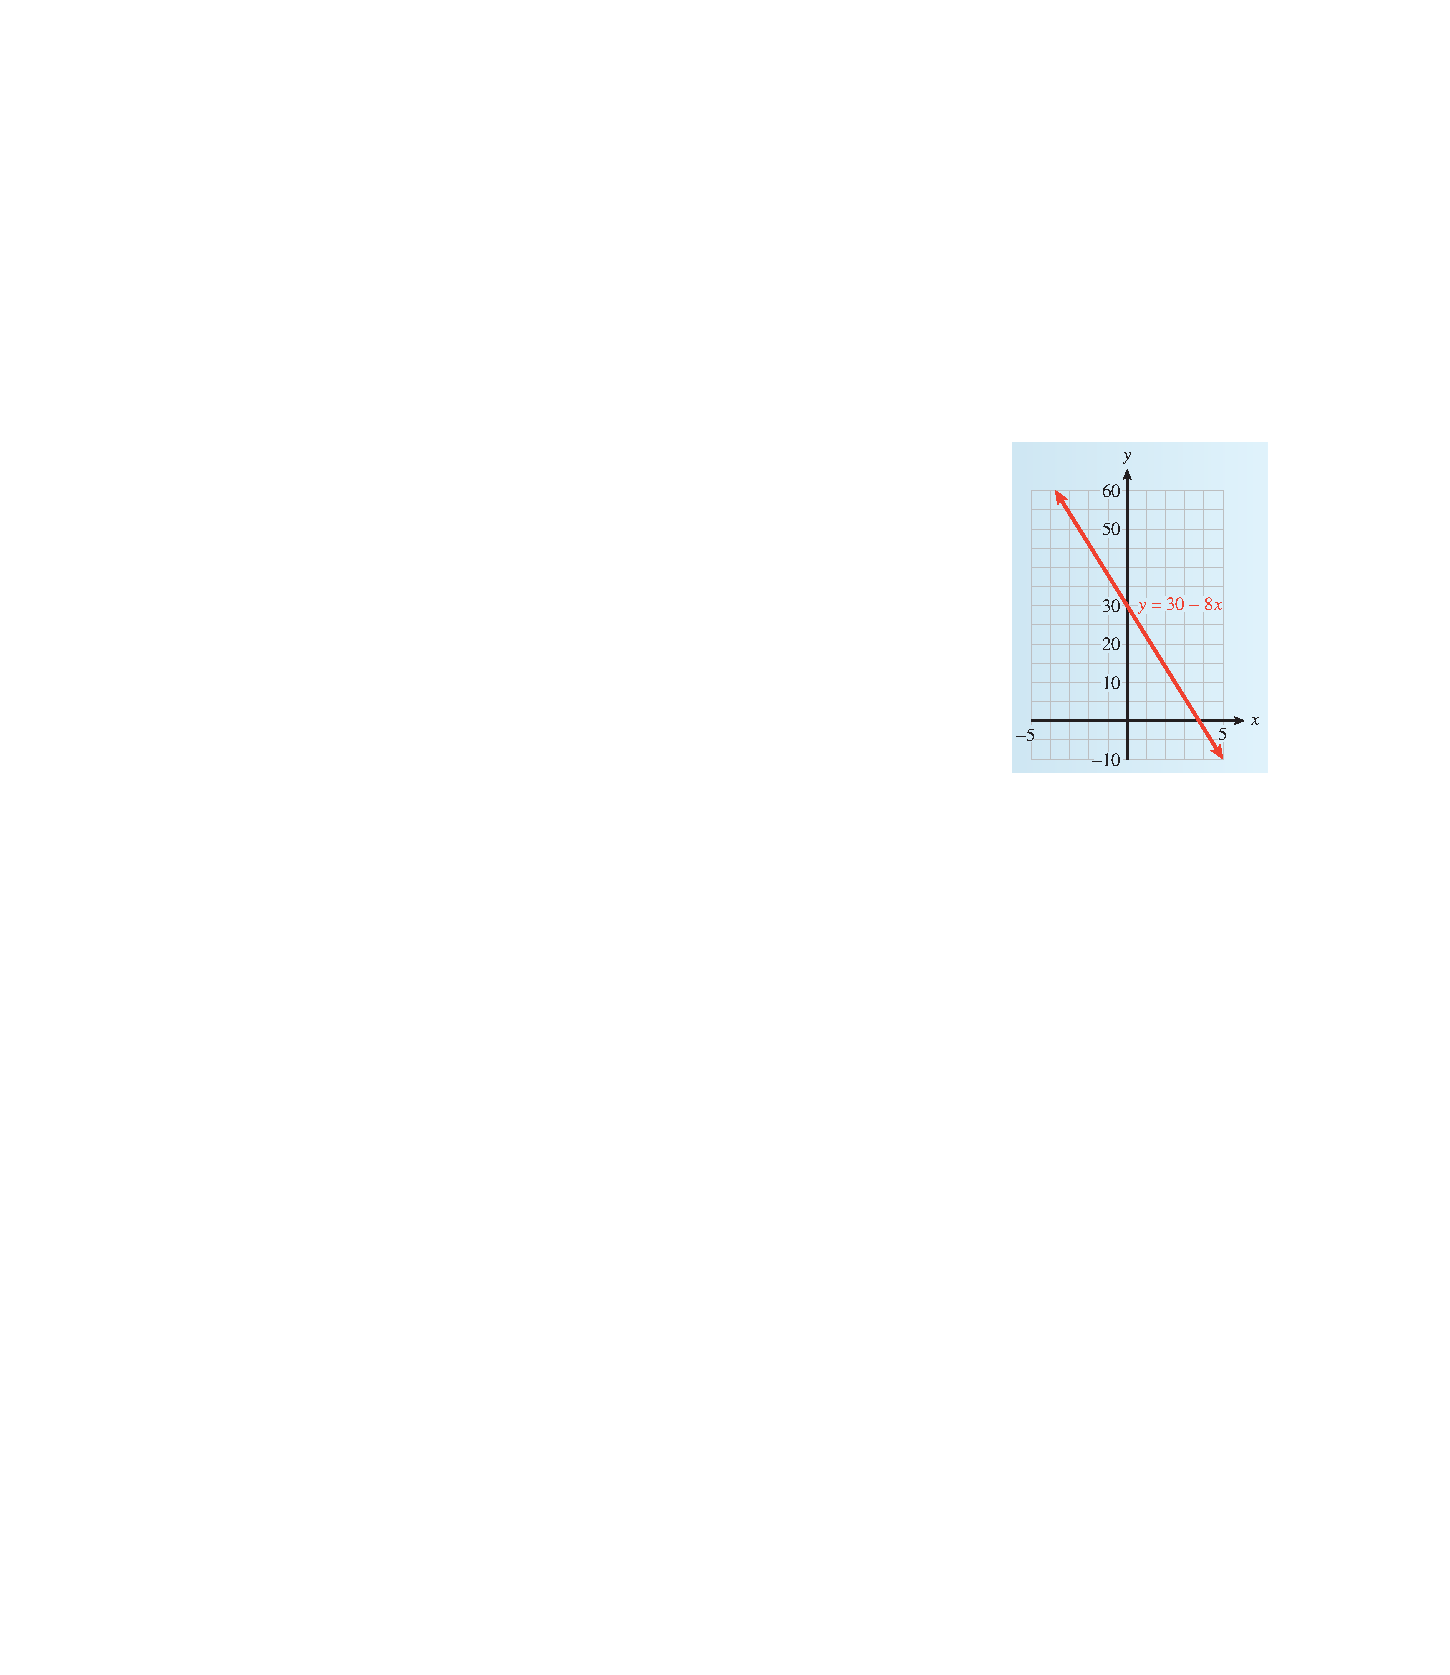
\includegraphics[width=0.50\textwidth,]{images/fig-graph-to-solve2.pdf}\caption{\label{fig-graph-to-solve2}}
\end{figure}
\end{exercise}
\leavevmode%
\begin{figure}
\centering
\pushValignCaptionBottom[b]{minipage}{.70\textwidth}{%
\parbox{\textwidth}{%
% horizontal alignment 
In a similar fashion, we can solve inequalities with a graph. Consider again the graph of \(y = 2x + 3\), shown in \hyperref[fig-graph-to-solve3]{Figure~\ref{fig-graph-to-solve3}}. We saw that \(x = 2\) is the solution of the equation \(2x + 3 = 7\). When we use \(x = 2\) as the input for the function \(f(x) = 2x + 3\), the output is \(y = 7\). Which input values for \(x\) produce output values greater than \(7\)? You can see in \hyperref[fig-graph-to-solve3]{Figure~\ref{fig-graph-to-solve3}} that \(x\)-values greater than \(2\) produce \(y\)-values greater than \(7\), because points on the graph with \(x\)-values greater than \(2\) have \(y\)-values greater than \(7\). Thus, the solutions of the inequality \(2x + 3 \gt 7\) are \(x\gt 2\). You can verify this result by solving the inequality algebraically.}%
}% end body 
{}% caption 
\pushValignCaptionBottom[b]{minipage}{.30\textwidth}{%
\centering% horizontal alignment 
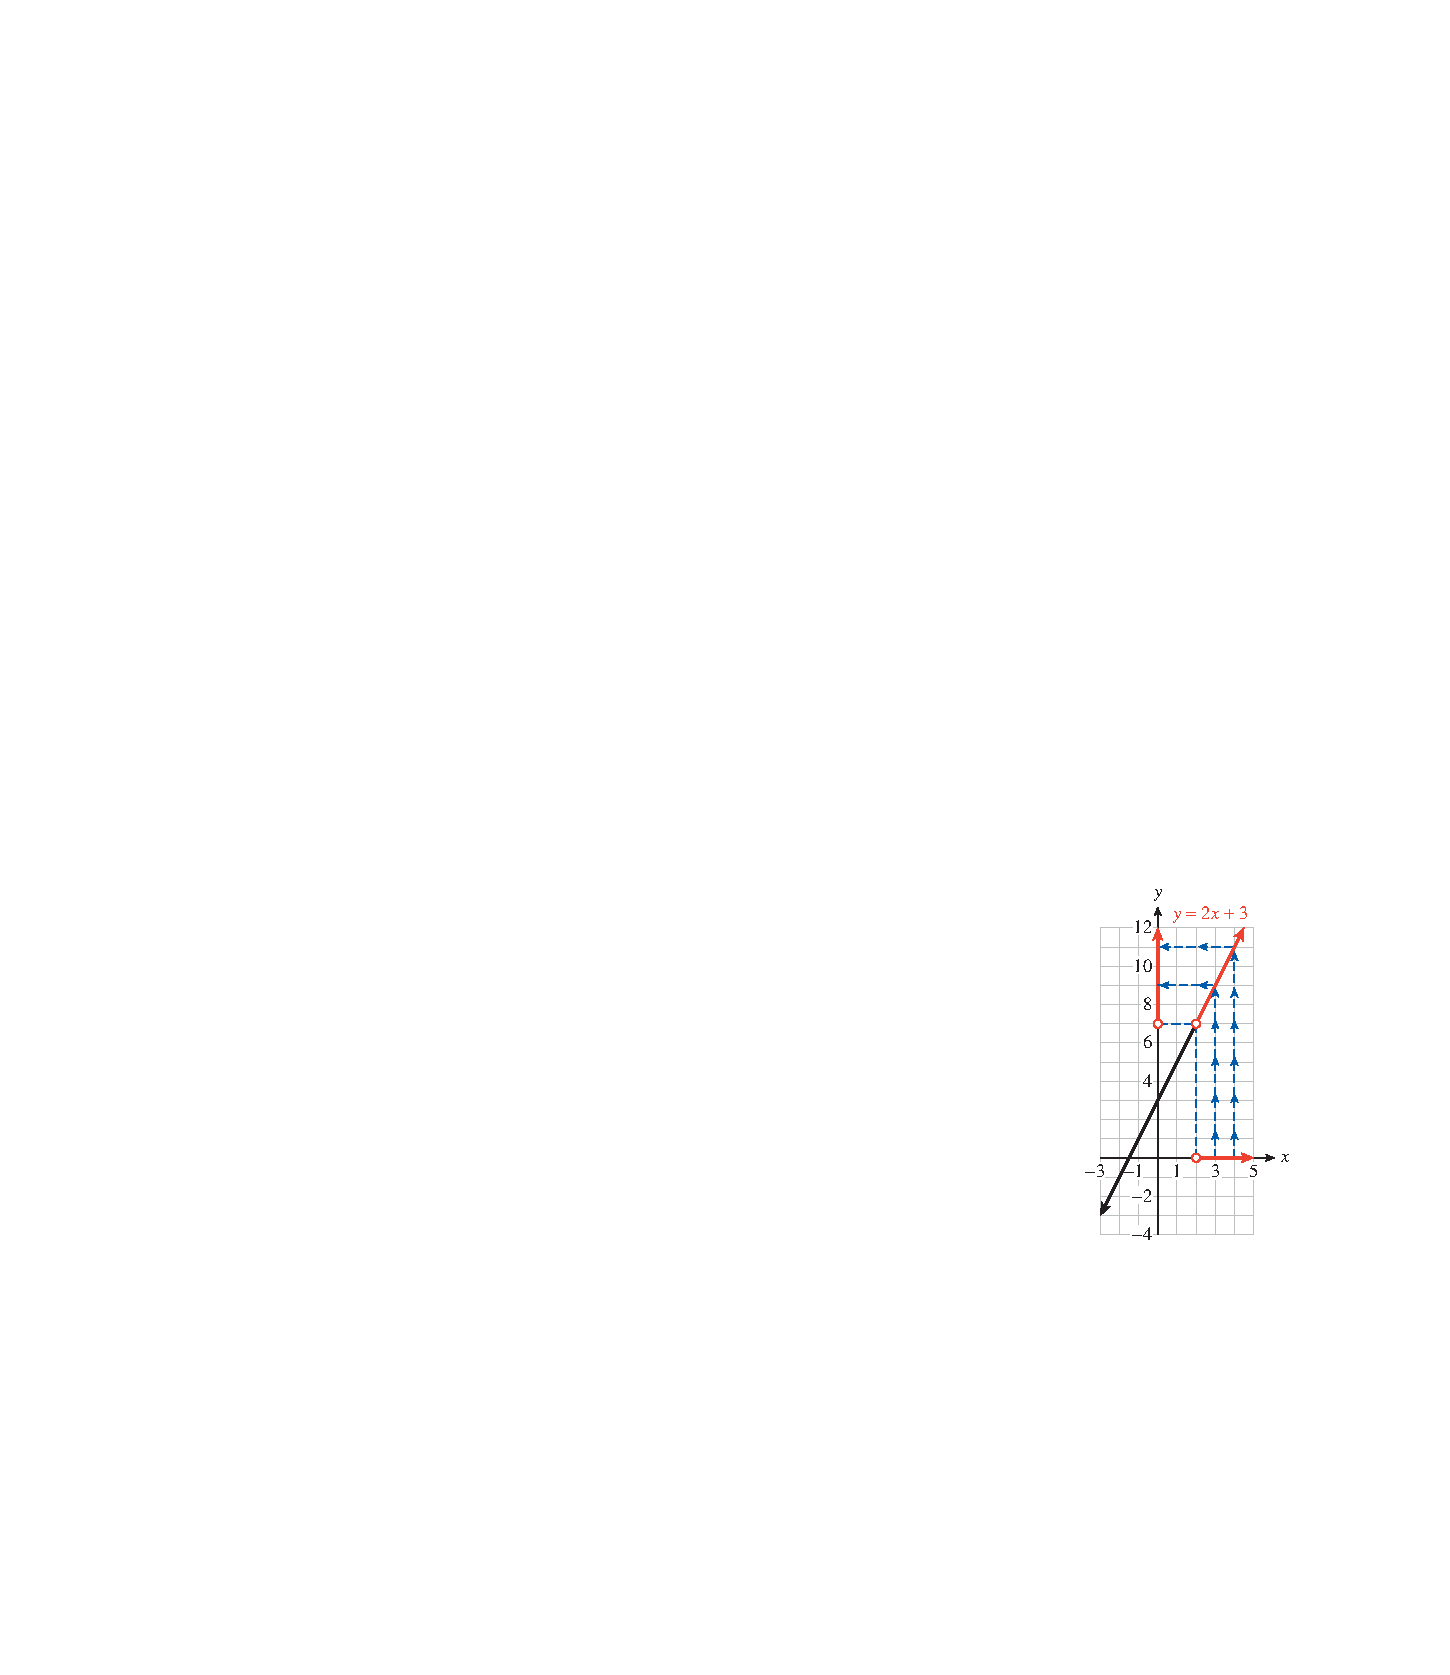
\includegraphics[width=\textwidth,]{images/fig-graph-to-solve3.pdf}}% end body 
{\captionof{figure}{\label{fig-graph-to-solve3}}
}% caption 
\popValignCaptionBottom
\end{figure}
\begin{example}[]\label{example-graph-to-solve2}
Use the graph of \(y = 285 − 15x\) to solve the inequality \begin{equation*}285 − 15x \gt 150\end{equation*}%
\par\medskip\noindent%
\textbf{Solution.}\quad 
    We begin by locating the point \(P\) on the graph for which \(y = 150\) and \(x = 9\) (its \(x\)-coordinate). Now, because \(y = 285 − 15x\) for points on the graph, the inequality \(285 − 15x \gt 150\) is equivalent to \(y \gt 150\). So we are looking for points on the graph with \(y\)-coordinate greater than \(150\). These points are shown in \hyperref[fig-graph-to-solve-inequality]{Figure~\ref{fig-graph-to-solve-inequality}}. The \(x\)-coordinates of these points are the \(x\)-values that satisfy the inequality. From the graph, we see that the solutions are \(x \lt 9\).
\leavevmode%
\begin{figure}
\centering
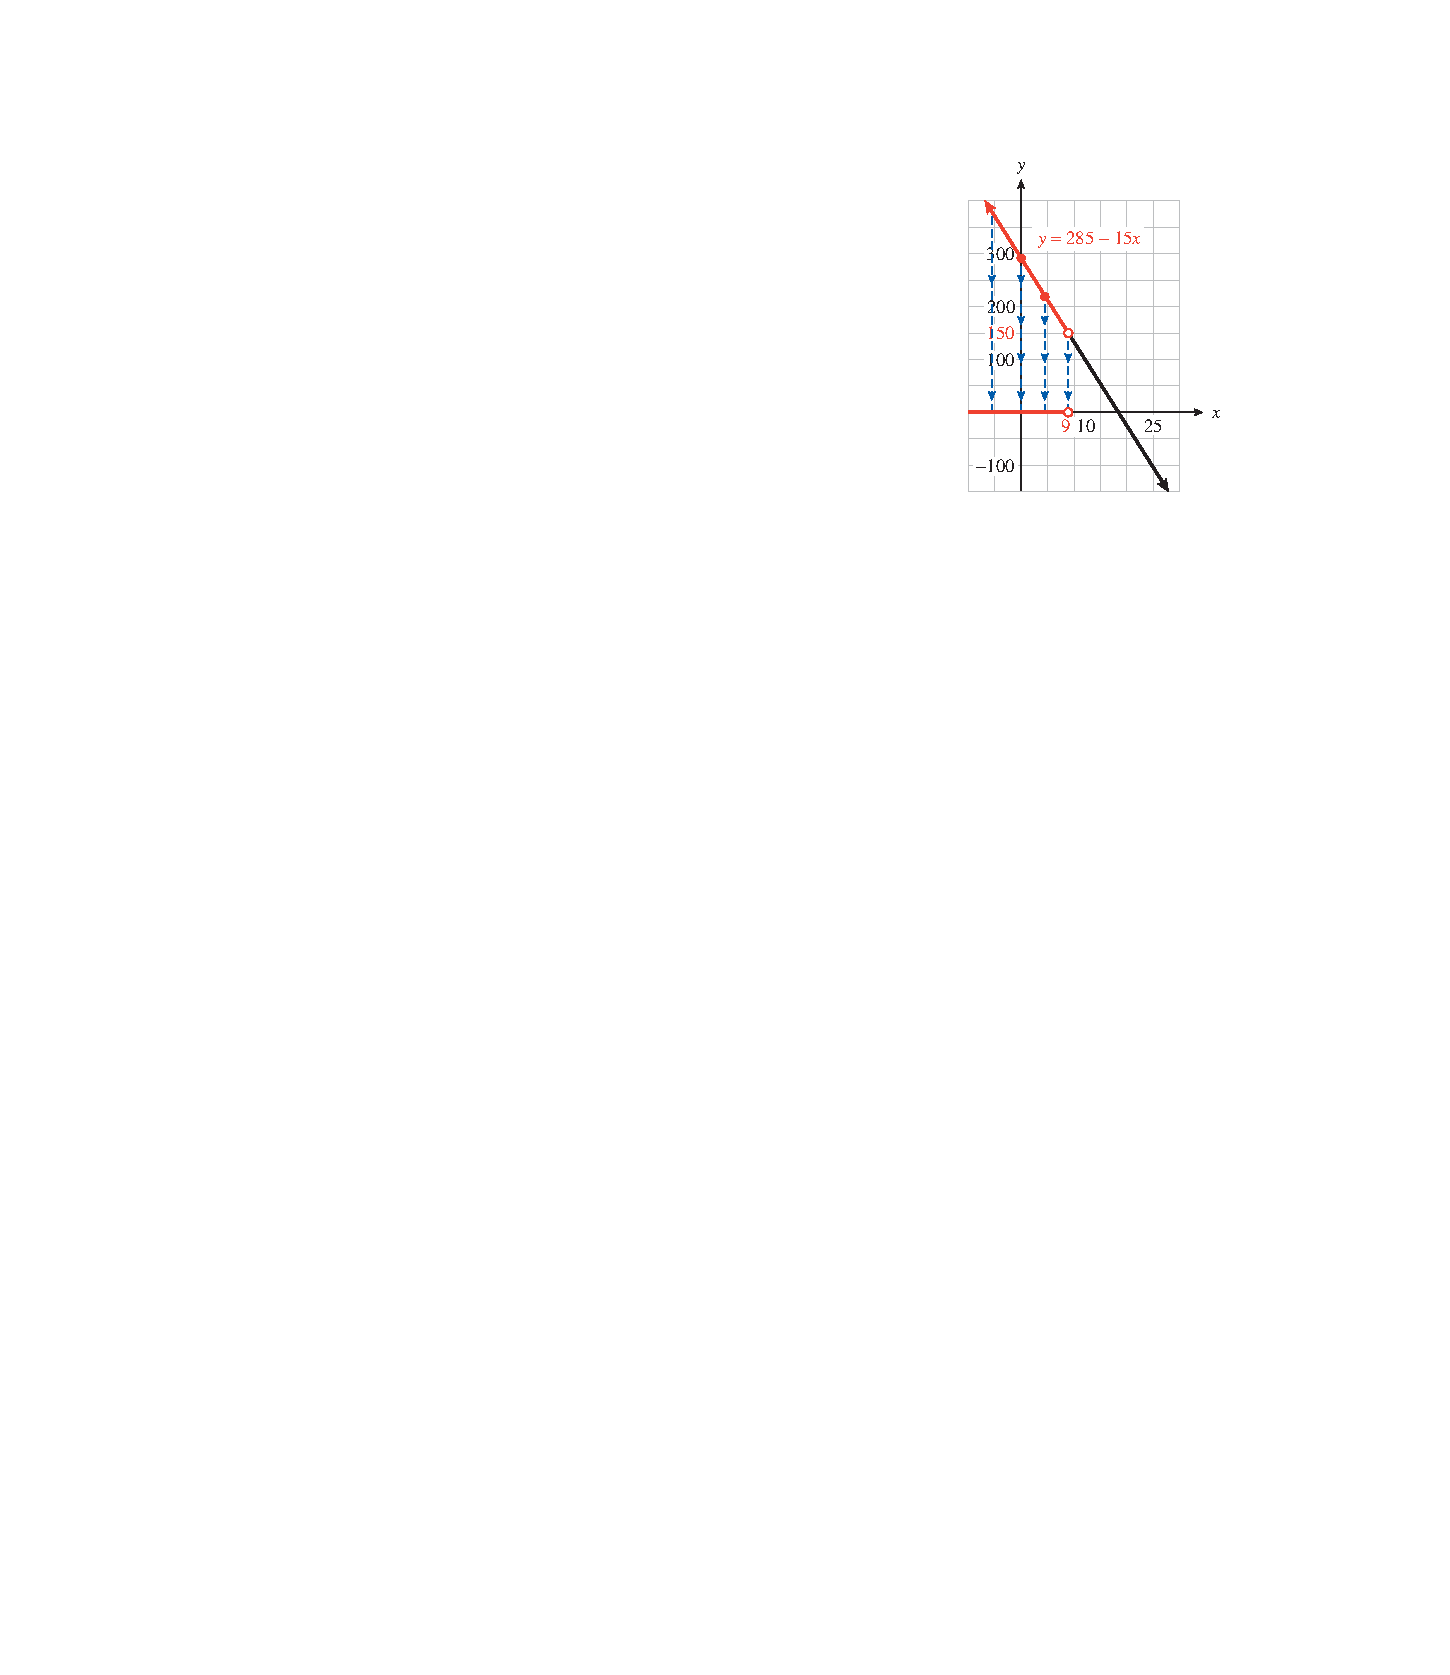
\includegraphics[width=0.60\textwidth,]{images/fig-graph-to-solve-inequality.pdf}\caption{\label{fig-graph-to-solve-inequality}}
\end{figure}
\end{example}
\begin{exercise}\label{exercise-graph-to-solve-inequality}
\leavevmode%
\begin{enumerate}[label=*\alph**]
\item\hypertarget{li-140}{}Use the graph of \(y = 30 − 8x\) in  \hyperref[fig-graph-to-solve2]{Figure~\ref{fig-graph-to-solve2}} to solve the inequality \begin{equation*}30 − 8x \le 50\end{equation*}\item\hypertarget{li-141}{}Solve the inequality algebraically.\end{enumerate}
\end{exercise}
\par
We can also use this graphical technique to solve nonlinear equations and inequalities.%
\begin{example}[]\label{example-graph-to-solve-cubic}
Use a graph of \(f(x) = −2x^3 + x^2 + 16x\) to solve the equation 
    \begin{equation*}−2x^3 + x^2 + 16x = 15\end{equation*}%
\par\medskip\noindent%
\textbf{Solution.}\quad If we sketch in the horizontal line \(y = 15\), we can see that there are three points on the graph of \(f\) that have \(y\)-coordinate \(15\), as shown in \hyperref[fig-graph-to-solve-cubic]{Figure~\ref{fig-graph-to-solve-cubic}}. The \(x\)-coordinates of these points are the solutions of the equation %
\par
\begin{equation*}−2x^3 + x^2 + 16x = 15\end{equation*}
    From the graph, we see that the solutions are \(x = −3\), \(x = 1\), and approximately \(x = 2.5\). We can verify the solutions algebraically. For example, if \(x = \alert{−3}\), we have 
    \begin{align*}
        f(\alert{−3})\&−2(\alert{−3})3 + (\alert{−3})^2 + 16(\alert{−3})\textbackslash{}\textbackslash{}
        \&= −2(−27) + 9 − 48\textbackslash{}\textbackslash{}
        \&=54 + 9 − 48 = 15  
    \end{align*}
    so \(−3\) is a solution.%
\leavevmode%
\begin{figure}
\centering
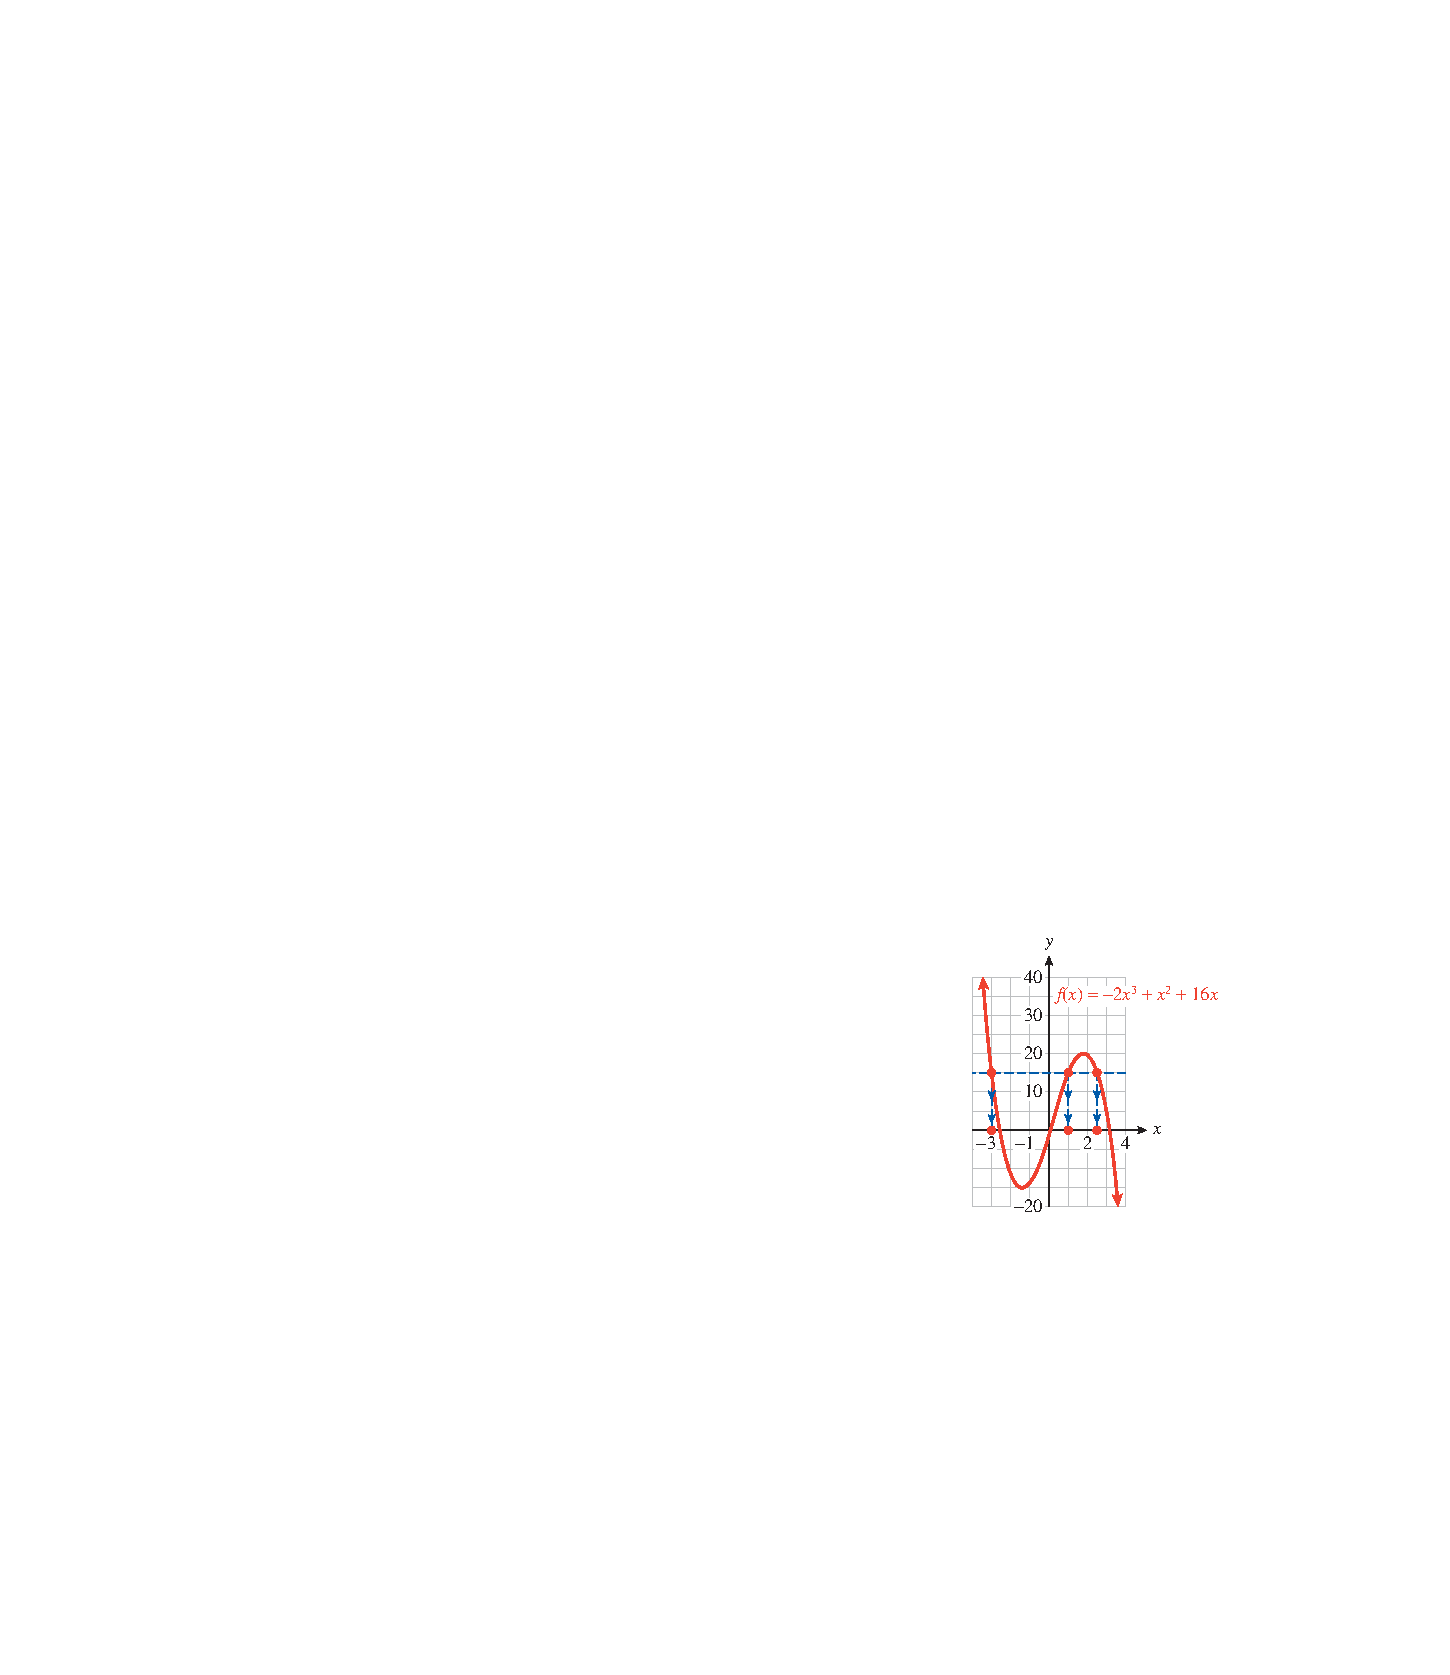
\includegraphics[width=0.90\textwidth,]{images/fig-graph-to-solve-cubic.pdf}\caption{\label{fig-graph-to-solve-cubic}}
\end{figure}
\end{example}
\begin{exercise}\label{exercise-graph-to-solve-quadratic}

    Use the graph of \(y = \frac{1}{2}n^2 + 2n − 10\) shown in \hyperref[fig-graph-to-solve-quadratic]{Figure~\ref{fig-graph-to-solve-quadratic}} to solve
    \begin{equation*}\frac{1}{2}n^2 + 2n − 10 = 6\end{equation*}
    and verify your solutions algebraically.
\leavevmode%
\begin{figure}
\centering
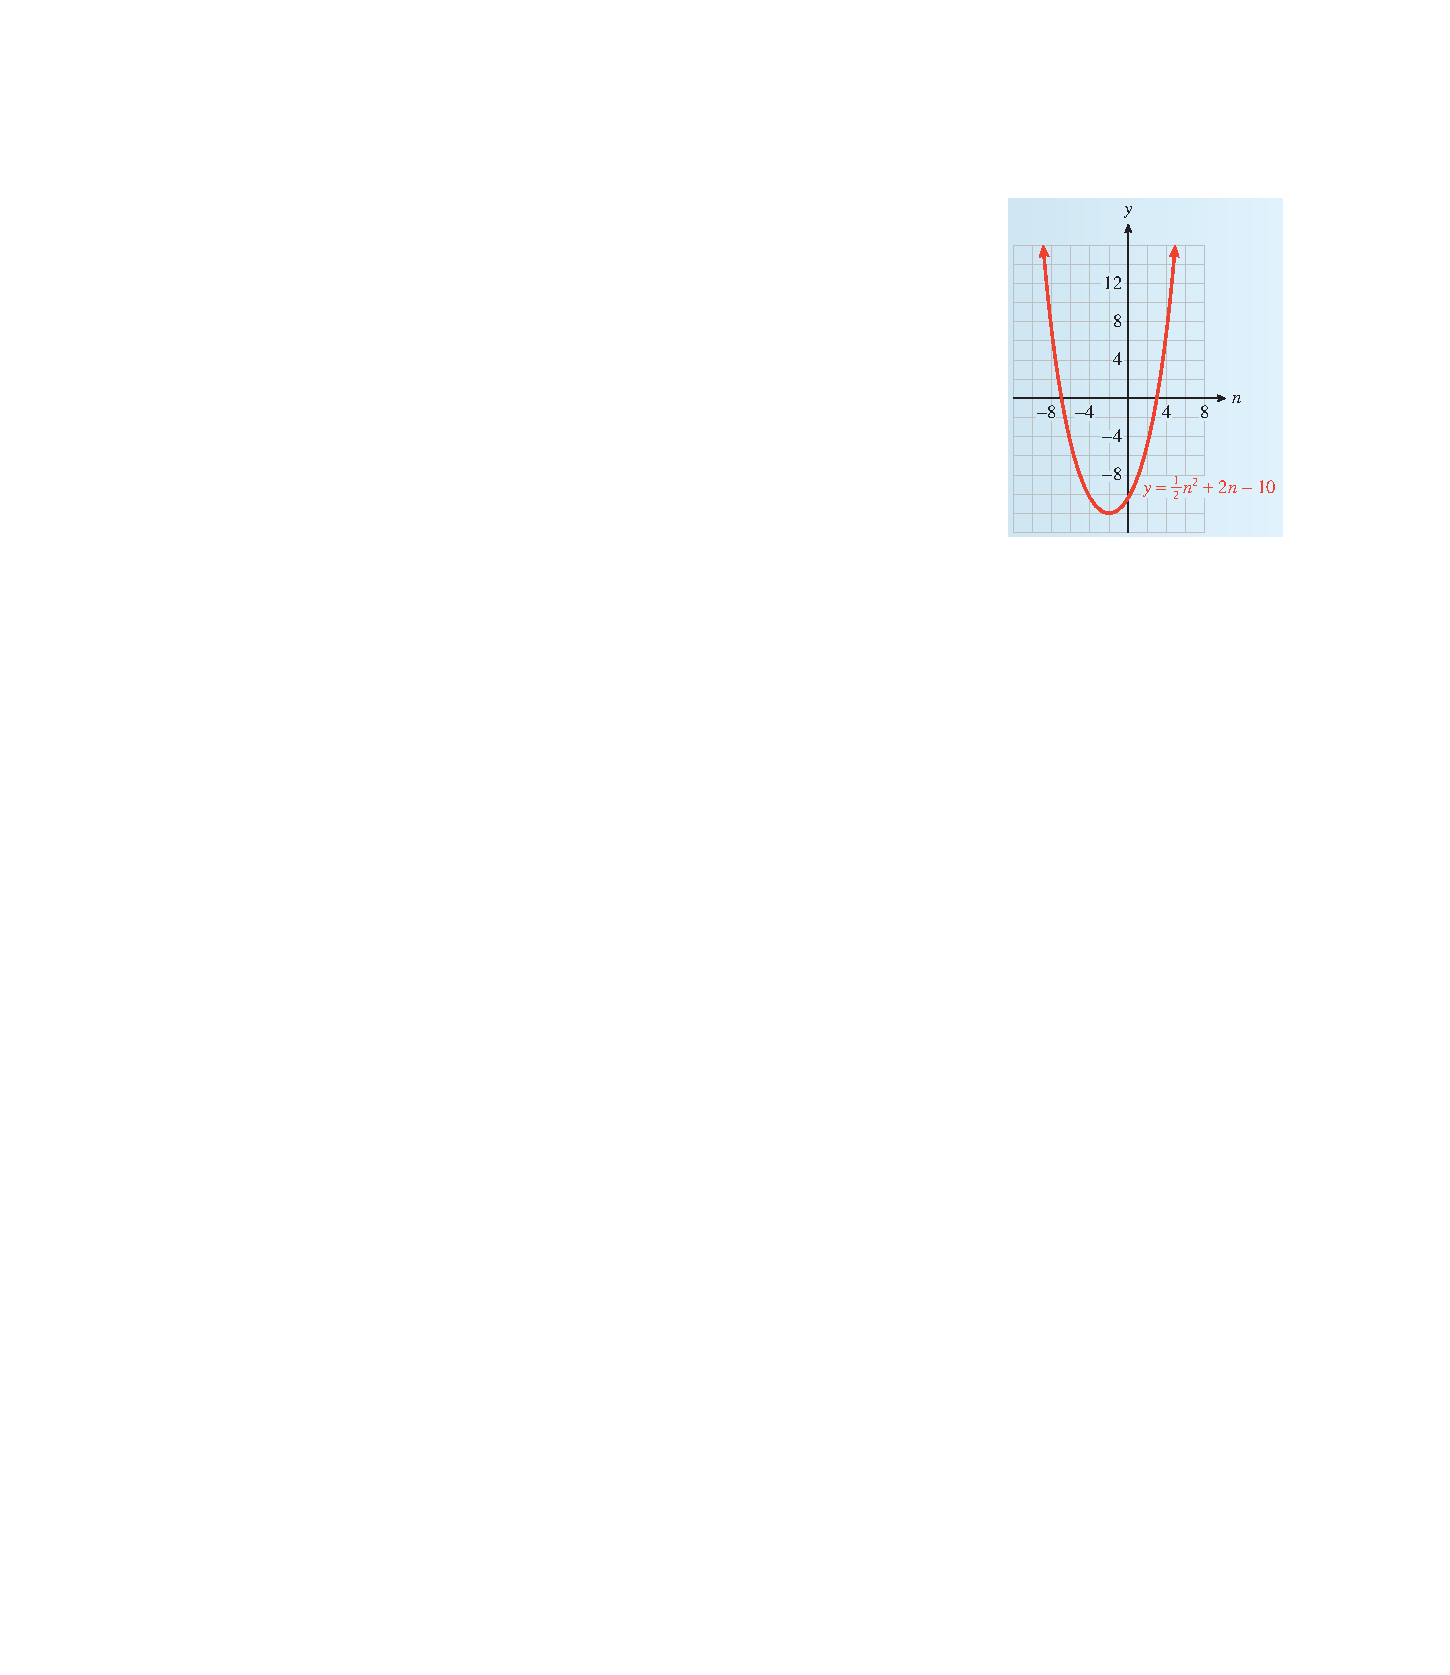
\includegraphics[width=0.60\textwidth,]{images/fig-graph-to-solve-quadratic.pdf}\caption{\label{fig-graph-to-solve-quadratic}}
\end{figure}
\end{exercise}
\begin{remark}[
\includegraphics[width=0.8\textwidth,]{images/icon-GC.pdf}Using the Trace Feature]\label{remark-7}
You can use the Trace feature on a graphing calculator to approximate solutions to equations. Graph the function \(f(x)\) in \hyperref[example-graph-to-solve-cubic]{Example~\ref{example-graph-to-solve-cubic}}  in the window
    \leavevmode%
\begin{table}
\centering
\begin{tabular}{lll}
Xmin\(=-4\)&&Xmax\(=4\)\tabularnewline[0pt]
Ymin\(=-20\)&&Ymax\(=40\)
\end{tabular}
\end{table}

    and trace along the curve to the point \((2.4680851, 15.512401)\). We are close to a solution, because the \(y\)-value is close to \(15\). Try entering \(x\)-values close to \(2.4680851\), for instance, \(x = 2.4\) and \(x = 2.5\), to find a better approximation for the solution.
%
\par

    We can use the intersect feature on a graphing calculator to obtain more accurate estimates for the solutions of equations. See {$\langle\langle$appendix-b$\rangle\rangle$} for details.
%
\end{remark}
\begin{example}[]\label{example-graph-to-solve-cubic2}
Use the graph in \hyperref[example-graph-to-solve-cubic]{Example~\ref{example-graph-to-solve-cubic}}  to solve the inequality
    \begin{equation*}−2x^3 + x^2 + 16x \ge 15\end{equation*}%
\par\medskip\noindent%
\textbf{Solution.}\quad 
        We first locate all points on the graph that have \(y\)-coordinates greater than or equal to \(15\). The \(x\)-coordinates of these points are the solutions of the inequality. \hyperref[fig-graph-to-solve-cubic2]{Figure~\ref{fig-graph-to-solve-cubic2}} shows the points, and their \(x\)-coordinates as intervals on the \(x\)-axis. The solutions are \(x \le −3\) and \(1\le x \le 2.5\), or in interval notation, \((-∞, −3] ∪ [1, 2.5]\).
        \leavevmode%
\begin{figure}
\centering
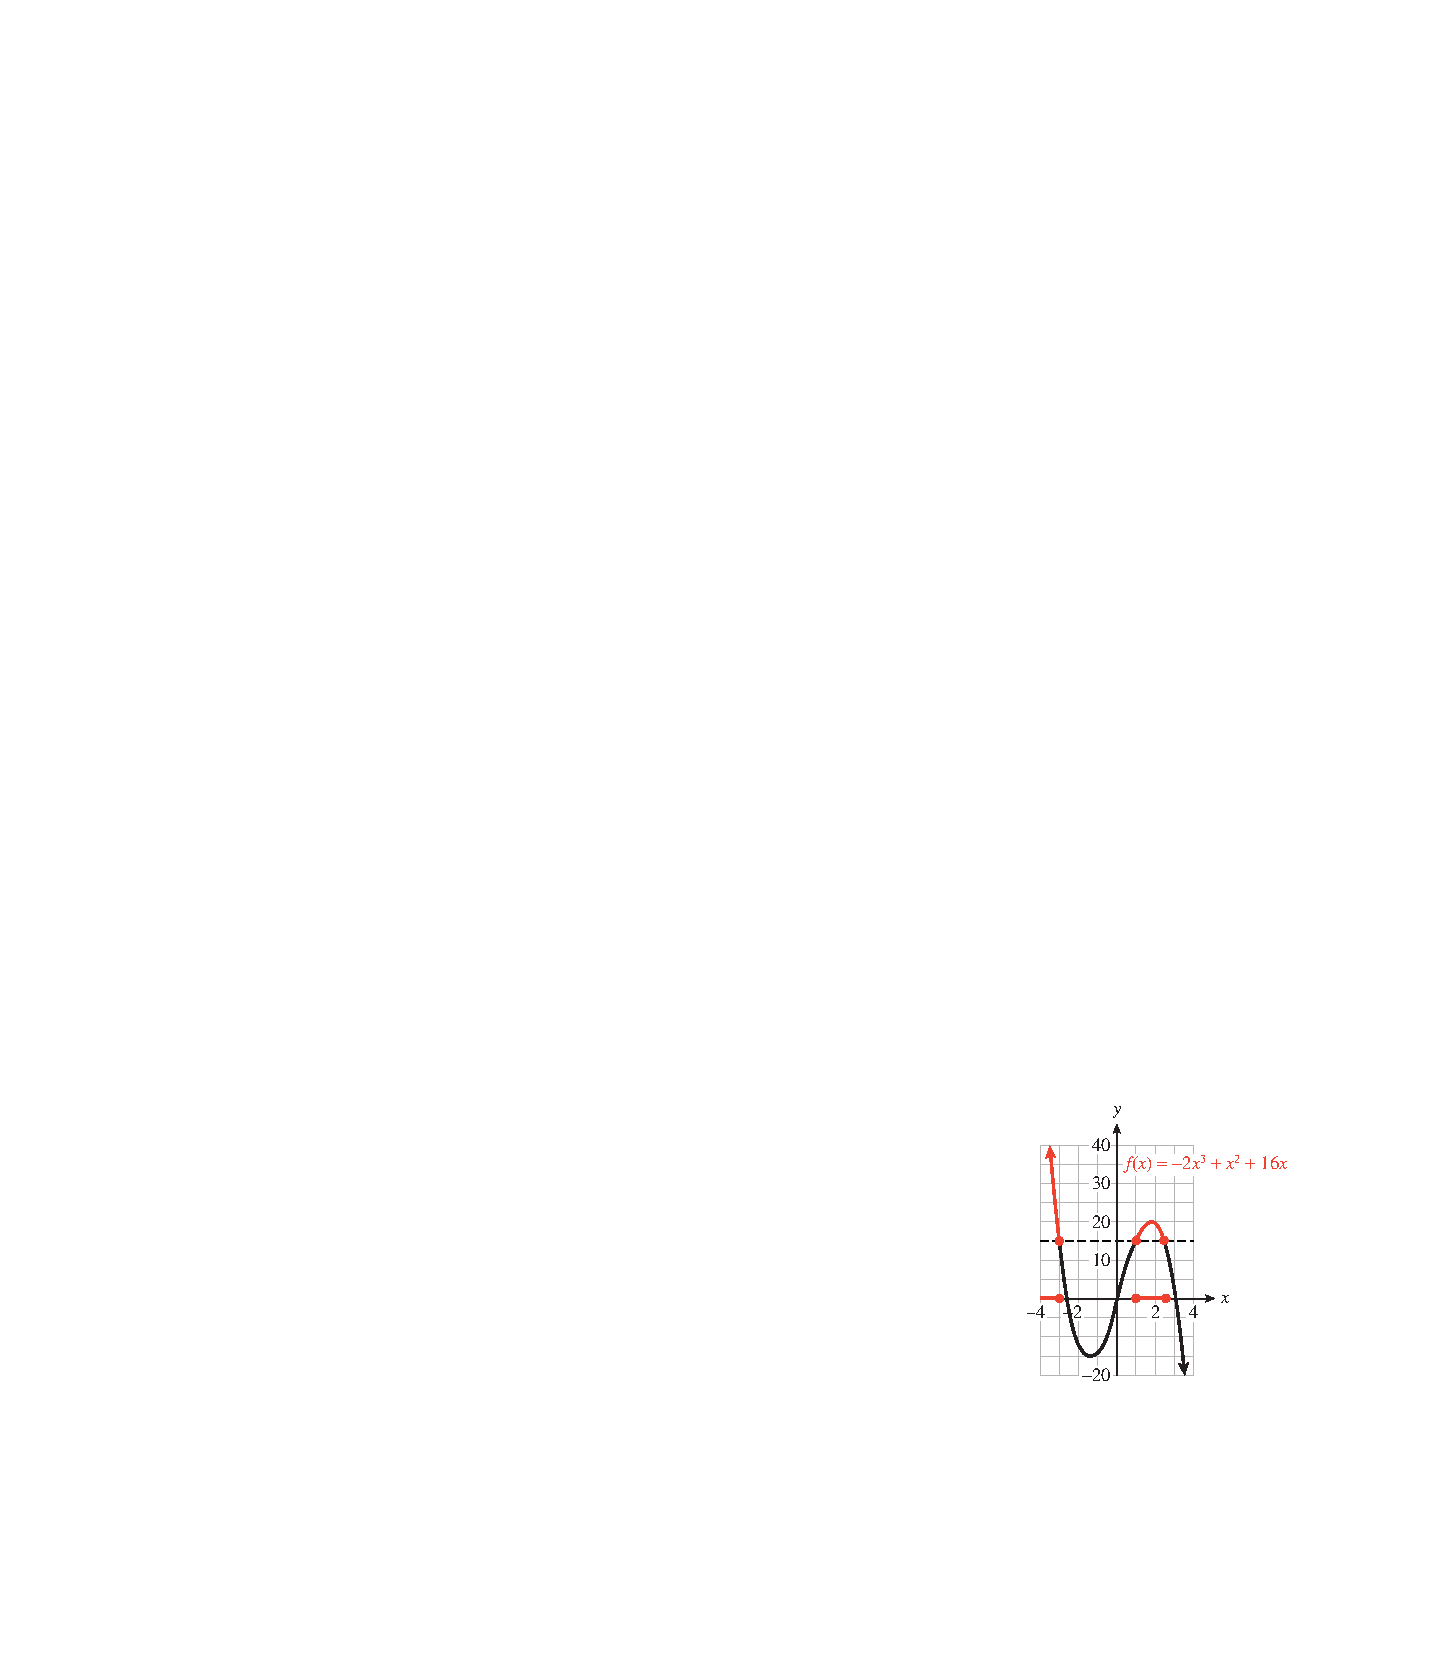
\includegraphics[width=0.60\textwidth,]{images/fig-graph-to-solve-cubic2.pdf}\caption{\label{fig-graph-to-solve-cubic2}}
\end{figure}
\end{example}
\begin{exercise}\label{exercise-graph-to-solve-quadratic2}
Use \hyperref[fig-graph-to-solve-quadratic]{Figure~\ref{fig-graph-to-solve-quadratic}} in \hyperref[exercise-graph-to-solve-quadratic]{Exercise~\ref{exercise-graph-to-solve-quadratic}} to solve the inequality
    \begin{equation*}\frac{1}{2}n^2 + 2n − 10 \lt 6\end{equation*}\end{exercise}
\typeout{************************************************}
\typeout{Section 1.4 Slope and Rate of Change}
\typeout{************************************************}
\section[Slope and Rate of Change]{Slope and Rate of Change}\label{slope-and-rate-of-change}
\typeout{************************************************}
\typeout{Subsection 1.4.1 Using Ratios for Comparison}
\typeout{************************************************}
\subsection[Using Ratios for Comparison]{Using Ratios for Comparison}\label{subsection-17}
Which is more expensive, a 64-ounce bottle of Velvolux dish soap that costs \textdollar{}3.52, or a 60-ounce bottle of Rainfresh dish soap that costs \textdollar{}3.36?%
\par
You are probably familiar with the notion of comparison shopping. To decide which dish soap is the better buy, we compute the unit price, or price per ounce, for each bottle. The unit price for Velvolux is
    \begin{equation*}\frac{352 \text{ cents}}{64 \text{ ounces}}= 5.5 \text{ cents per ounce}\end{equation*}
and the unit price for Rainfresh is
    \begin{equation*}\frac{336 \text{ cents}}{60 \text{ ounces}}= 5.6 \text{ cents per ounce}\end{equation*}
%
\par

    The Velvolux costs less per ounce, so it is the better buy. By computing the price of each brand for \emph{the same amount of soap}, it is easy to compare them.%
\par

    In many situations, a ratio, similar to a unit price, can provide a basis for comparison. \hyperref[example-rate-of-growth]{Example~\ref{example-rate-of-growth}} uses a ratio to measure a rate of growth.
%
\begin{example}[]\label{example-rate-of-growth}
Which grow faster, Hybrid A wheat seedlings, which grow 11.2 centimeters in 14 days, or Hybrid B seedlings, which grow 13.5 centimeters in 18 days?%
\par\medskip\noindent%
\textbf{Solution.}\quad 
    We compute the growth rate for each strain of wheat. Growth rate is expressed as a ratio, \(\frac{\text{centimeters}}{\text{days}}\), or centimeters per day. The growth rate for Hybrid A is
    \begin{equation*}\frac{11.2 \text{ centimeters}}{14 \text{ days}}= 0.8 \text{ centimeters per day}\end{equation*}
and the growth rate for Hybrid B is
    \begin{equation*}\frac{13.5 \text{ centimeters}}{18 \text{ days}}= 0.75 \text{ centimeters per day}\end{equation*}
Because their rate of growth is larger, the Hybrid A seedlings grow faster.
\end{example}
\par

    By computing the growth of each strain of wheat seedling over the same unit of time, a single day, we have a basis for comparison. In this case, the ratio \(\frac{\text{centimeters}}{\text{day}}\) measures the rate of growth of the wheat seedlings.
%
\begin{exercise}\label{exercise-gas-mileage}

    Delbert traveled 258 miles on 12 gallons of gas, and Francine traveled 182 miles on 8 gallons of gas. Compute the ratio \(\frac{\text{miles}}{\text{gallon}}\) for each car. Whose car gets the better gas mileage?
\end{exercise}
\par

    In \hyperref[exercise-gas-mileage]{Exercise~\ref{exercise-gas-mileage}}, the ratio \(\frac{\text{miles}}{\text{gallon}}\) measures the rate at which each car uses gasoline. By computing the mileage for each car for the same amount of gas, we have a basis for comparison. We can use this same idea, finding a common basis for comparison, to measure the steepness of an incline.
%
\typeout{************************************************}
\typeout{Subsection 1.4.2 Measuring Steepness}
\typeout{************************************************}
\subsection[Measuring Steepness]{Measuring Steepness}\label{subsection-18}
Imagine you are an ant carrying a heavy burden along one of the two paths shown in \hyperref[fig-ant-climb]{Figure~\ref{fig-ant-climb}}. Which path is more difficult? Most ants would agree that the steeper path is more difficult. %
\leavevmode%
\begin{figure}
\centering
\pushValignCaptionBottom[b]{minipage}{.50\textwidth}{%
\parbox{\textwidth}{%
% horizontal alignment 
But what exactly is steepness? It is not merely the gain in altitude, because even a gentle incline will reach a great height eventually. Steepness measures how sharply the altitude increases. An ant finds the second path more difficult, or steeper, because it rises 5 feet while the first path rises only 2 feet over the same horizontal distance.}%
}% end body 
{}% caption 
\pushValignCaptionBottom[b]{minipage}{.50\textwidth}{%
\centering% horizontal alignment 
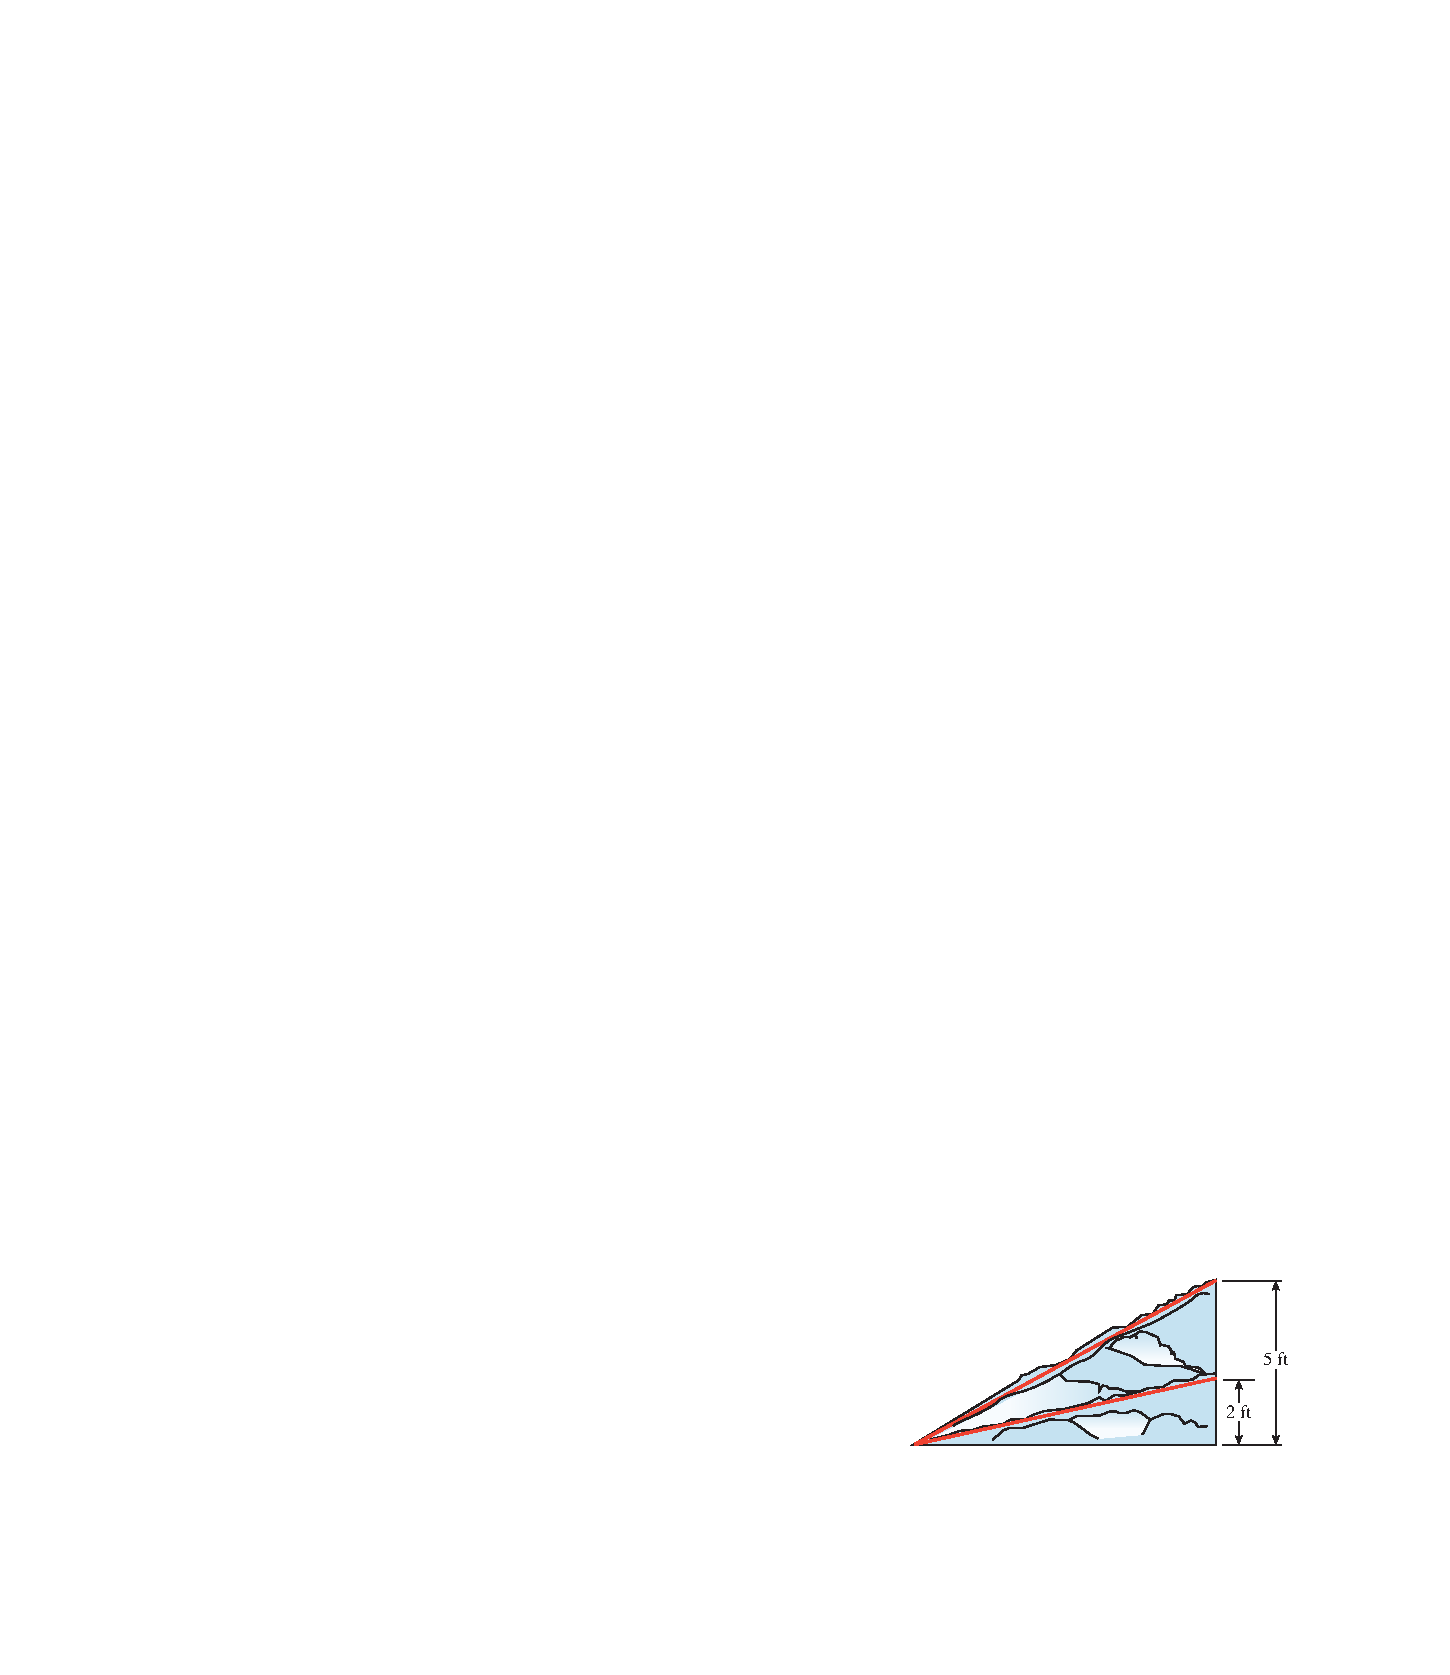
\includegraphics[width=\textwidth,]{images/fig-ant-climb.pdf}}% end body 
{\captionof{figure}{\label{fig-ant-climb}}
}% caption 
\popValignCaptionBottom
\end{figure}
\par
To compare the steepness of two inclined paths, we compute the ratio of change in
altitude to change in horizontal distance for each path.%
\begin{example}[]\label{example-steep-trail}
Which is steeper, Stony Point trail, which climbs 400 feet over a horizontal distance of 2500 feet, or Lone Pine trail, which climbs 360 feet over a horizontal distance of 1800 feet?%
\par\medskip\noindent%
\textbf{Solution.}\quad For each trail, we compute the ratio of vertical gain to horizontal distance. For Stony Point trail, the ratio is
    \begin{equation*}\frac{400 \text{ feet}}{2500 \text{ feet}}= 0.16 \end{equation*}  
    and for Lone Pine trail, the ratio is
    \begin{equation*}\frac{360 \text{ feet}}{1800 \text{ feet}}= 0.20 \end{equation*} 
    Lone Pine trail is steeper, because it has a vertical gain of 0.20 foot for every foot traveled horizontally. Or, in more practical units, Lone Pine trail rises 20 feet for every 100 feet of horizontal distance, whereas Stony Point trail rises only 16 feet over a horizontal distance of 100 feet.%
\end{example}
\begin{exercise}\label{exercise-steep-steps}
Which is steeper, a staircase that rises 10 feet over a horizontal distance of 4 feet, or the steps in the football stadium, which rise 20 yards over a horizontal distance of 12 yards?\end{exercise}
\typeout{************************************************}
\typeout{Subsection 1.4.3 Definition of Slope}
\typeout{************************************************}
\subsection[Definition of Slope]{Definition of Slope}\label{subsection-19}

    To compare the steepness of the two trails in \hyperref[example-steep-trail]{Example~\ref{example-steep-trail}}, it is not enough to know which trail has the greater gain in elevation overall. Instead, we compare their elevation gains over the same horizontal distance. Using the same horizontal distance provides a basis for comparison. The two trails are illustrated in \hyperref[fig-trail-climb-grid]{Figure~\ref{fig-trail-climb-grid}} as lines on a coordinate grid.
%
\leavevmode%
\begin{figure}
\centering
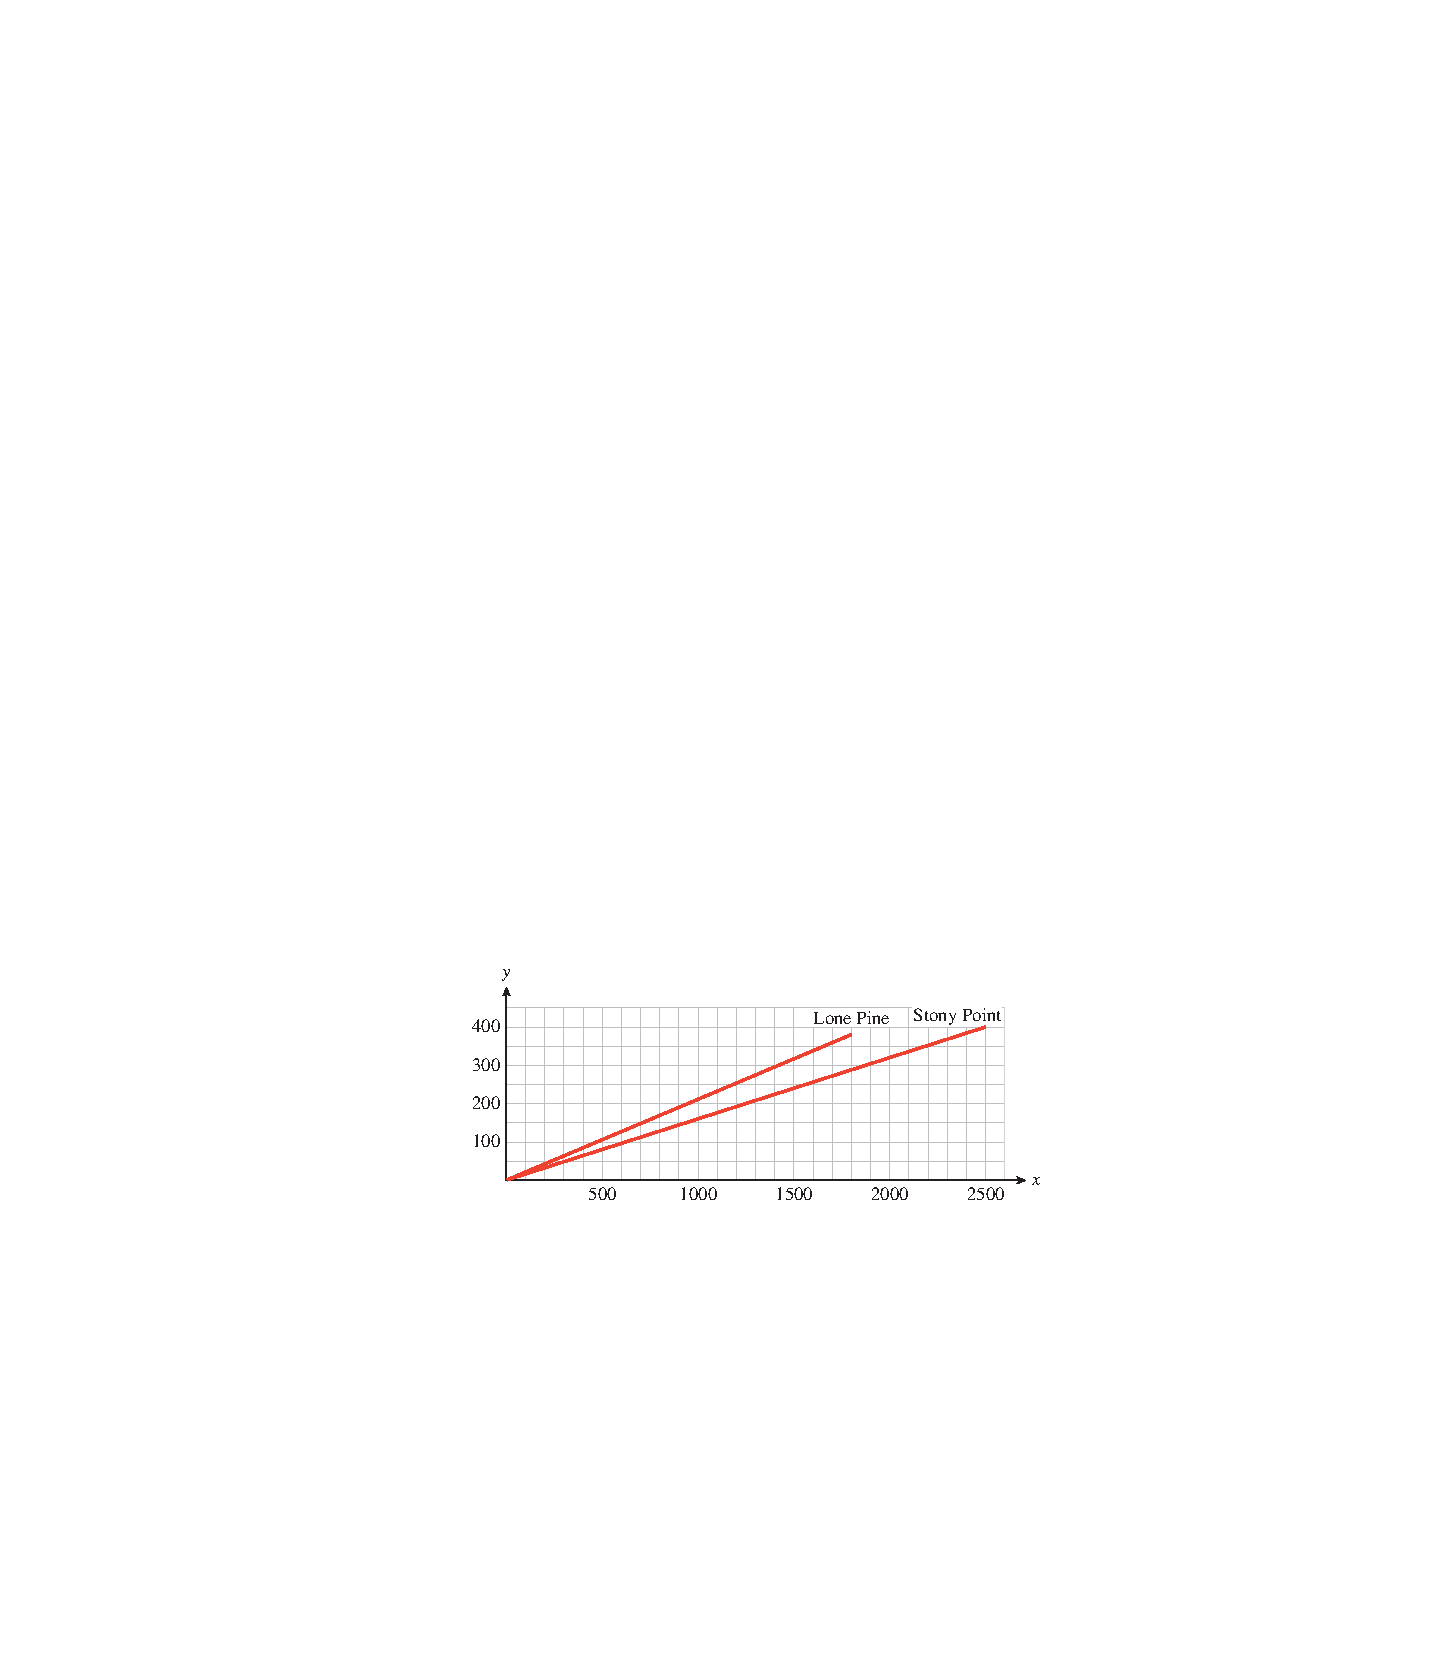
\includegraphics[width=0.90\textwidth,]{images/fig-trail-climb-grid.pdf}\caption{\label{fig-trail-climb-grid}}
\end{figure}
\par

    The ratio we computed in \hyperref[example-steep-trail]{Example~\ref{example-steep-trail}},
    \begin{equation*}\frac{\text{change in elevation}}{\text{change in horizontal position}}\end{equation*}  
    appears on the graphs in \hyperref[fig-trail-climb-grid]{Figure~\ref{fig-trail-climb-grid}} as
    \begin{equation*}\frac{\text{change in }y\text{-coordinate}}{\text{change in }x\text{-coordinate}}\end{equation*} 
    For example, as we travel along the line representing Stony Point trail, we move from the point\(0, 0)\) to the point \((2500, 400)\). The \(y\)-coordinate changes by \(400\) and the \(x\)-coordinate changes by \(2500\), giving the ratio \(0.16\) that we found in \hyperref[example-steep-trail]{Example~\ref{example-steep-trail}}2. We call this ratio the \terminology{slope} of the line.
%
\begin{definition}[]\label{definition-slope}
The \terminology{slope} of a line is the ratio
    \begin{equation*}\frac{\text{change in }y\text{-coordinate}}{\text{change in }x\text{-coordinate}}\end{equation*} 
    as we move from one point to another on the line.
    %
\end{definition}
\begin{example}[]\label{example-slope-grid}

    Compute the slope of the line that passes through points \(A\) and \(B\) in \hyperref[fig-slope-grid]{Figure~\ref{fig-slope-grid}}.
%
\leavevmode%
\begin{figure}
\centering
\includegraphics[width=0.50\textwidth,]{images/fig-slope-grid.pdf}\caption{\label{fig-slope-grid}}
\end{figure}
\par\medskip\noindent%
\textbf{Solution.}\quad 
    As we move along the line from \(A\) to \(B\), the \(y\)-coordinate changes by \(3\) units, and the \(x\)-coordinate changes by \(4\) units. The slope of the line is thus
    \begin{equation*}\frac{\text{change in }y\text{-coordinate}}{\text{change in }x\text{-coordinate}}=\frac{3}{4}\end{equation*}\end{example}
\begin{exercise}\label{exercise-slope-grid}
\leavevmode%
\begin{figure}
\centering
\pushValignCaptionBottom[b]{minipage}{.50\textwidth}{%
\parbox{\textwidth}{%
% horizontal alignment 
Compute the slope of the line through the indicated points in \hyperref[fig-slope-grid2]{Figure~\ref{fig-slope-grid2}}. On both axes, one square represents one unit. 
    \begin{equation*}\frac{\text{change in }y\text{-coordinate}}{\text{change in }x\text{-coordinate}}=\end{equation*} 
    }%
}% end body 
{}% caption 
\pushValignCaptionBottom[b]{minipage}{.50\textwidth}{%
\centering% horizontal alignment 
\includegraphics[width=\textwidth,]{images/fig-slope-grid2.pdf}}% end body 
{\captionof{figure}{\label{fig-slope-grid2}}
}% caption 
\popValignCaptionBottom
\end{figure}
\end{exercise}
\par

    The slope of a line is a number. It tells us how much the \(y\)-coordinates of points on the line increase when we increase their \(x\)-coordinates by 1 unit. For instance, the slope \(\frac{3}{4}\) in \hyperref[example-slope-grid]{Example~\ref{example-slope-grid}} means that the \(y\)-coordinate increases by \(\frac{3}{4}\) unit when the \(x\)-coordinate increases by 1 unit. For increasing graphs, a larger slope indicates a greater increase in altitude, and hence a steeper line.
%
\typeout{************************************************}
\typeout{Subsection 1.4.4 Notation for Slope}
\typeout{************************************************}
\subsection[Notation for Slope]{Notation for Slope}\label{subsection-20}

    We use a shorthand notation for the ratio that defines slope,
    \begin{equation*}\frac{\text{change in }y\text{-coordinate}}{\text{change in }x\text{-coordinate}}\end{equation*} 
    The symbol \(\Delta\) (the Greek letter delta) is used in mathematics to denote \emph{change in}. In particular, \(\Delta y\) means \emph{change in \(y\)-coordinate}, and \(\Delta x\) means \emph{change in \(x\)-coordinate}. We also use the letter \(m\) to stand for slope. With these symbols, we can write the definition of slope as follows.
%
\typeout{************************************************}
\typeout{Paragraphs  Notation for Slope}
\typeout{************************************************}
\paragraph[Notation for Slope]{Notation for Slope}\label{paragraphs-11}
\leavevmode%
\begin{figure}
\centering
\pushValignCaptionBottom[b]{minipage}{.50\textwidth}{%
\parbox{\textwidth}{%
% horizontal alignment 

    The \terminology{slope} of a line is given by
    \begin{equation*}\frac{\Delta y}{\Delta x}=\frac{\text{change in }y\text{-coordinate}}{\text{change in }x\text{-coordinate}}\text{, }~x\ne 0\end{equation*} 
}%
}% end body 
{}% caption 
\pushValignCaptionBottom[b]{minipage}{.50\textwidth}{%
\centering% horizontal alignment 
\includegraphics[width=\textwidth,]{images/fig-slope-Delta.pdf}}% end body 
{}% caption 
\popValignCaptionBottom
\end{figure}
\begin{example}[]\label{example-Great-Pyramid}

        The Great Pyramid of Khufu in Egypt was built around 2550 B.C. It is 147 meters tall and has a square base 229 meters on each side. Calculate the slope of the sides of the pyramid, rounded to two decimal places.
    %
\par\medskip\noindent%
\textbf{Solution.}\quad \leavevmode%
\begin{figure}
\centering
\pushValignCaptionBottom[b]{minipage}{.50\textwidth}{%
\parbox{\textwidth}{%
% horizontal alignment 

            From \hyperref[fig-Great-Pyramid]{Figure~\ref{fig-Great-Pyramid}}, we see that \(\Delta x\) is only half the base of the Great Pyramid, so \begin{equation*}\Delta x = 0.5(229) = 114.5\end{equation*}
            and the slope of the side is 
            \begin{equation*}m=\frac{\Delta y}{\Delta x}= \frac{147}{114.5} = 1.28\end{equation*}
        }%
}% end body 
{}% caption 
\pushValignCaptionBottom[b]{minipage}{.50\textwidth}{%
\centering% horizontal alignment 
\includegraphics[width=\textwidth,]{images/fig-Great-Pyramid.pdf}}% end body 
{\captionof{figure}{\label{fig-Great-Pyramid}}
}% caption 
\popValignCaptionBottom
\end{figure}
\end{example}
\begin{exercise}\label{Kukulcan-pyramid}
\leavevmode%
\begin{figure}
\centering
\pushValignCaptionBottom[b]{minipage}{.50\textwidth}{%
\parbox{\textwidth}{%
% horizontal alignment 

        The Kukulcan Pyramid at Chichen Itza in Mexico was built around 800 A.D. It is 24 meters high, with a temple built on its top platform, as shown in \hyperref[fig-Kukulcan-Pyramid]{Figure~\ref{fig-Kukulcan-Pyramid}}. The square base is 55 meters on each side, and the top platform is 19.5 meters on each side. Calculate the slope of the sides of the pyramid. Which pyramid is steeper, Kukulcan or the Great Pyramid?
    }%
}% end body 
{}% caption 
\pushValignCaptionBottom[b]{minipage}{.50\textwidth}{%
\centering% horizontal alignment 
\includegraphics[width=\textwidth,]{images/fig-Kukulcan-Pyramid.pdf}}% end body 
{\captionof{figure}{\label{fig-Kukulcan-Pyramid}}
}% caption 
\popValignCaptionBottom
\end{figure}
\end{exercise}
\par

    So far, we have only considered examples in which \(\Delta x\) and \(\Delta y\) are positive numbers, but they can also be negative.
    \begin{equation*}\Delta x = \begin{cases}
        \text{positive if } x \text{ increases (move to the right)}\\
        \text{negative if } x \text{ decreases (move to the left)}\\
        \end{cases}
    \end{equation*}
    \begin{equation*}\Delta y = \begin{cases}
        \text{positive if } y \text{ increases (move up)}\\
        \text{negative if } y \text{ decreases (move down)}~~~~~~~~~\\
        \end{cases}
    \end{equation*}
%
\begin{example}[]\label{example-negative-slope}
\leavevmode%
\begin{figure}
\centering
\pushValignCaptionBottom[b]{minipage}{.50\textwidth}{%
\parbox{\textwidth}{%
% horizontal alignment 

        Compute the slope of the line that passes through the points \(P(−4, 2)\) and \(Q(5, −1)\) shown in \hyperref[fig-negative-slope]{Figure~\ref{fig-negative-slope}} Illustrate \(\Delta y\) and \(\Delta x\) on the graph.
    }%
}% end body 
{}% caption 
\pushValignCaptionBottom[b]{minipage}{.50\textwidth}{%
\centering% horizontal alignment 
\includegraphics[width=\textwidth,]{images/fig-negative-slope.pdf}}% end body 
{\captionof{figure}{\label{fig-negative-slope}}
}% caption 
\popValignCaptionBottom
\end{figure}
\par\medskip\noindent%
\textbf{Solution.}\quad 
        As we move from the point \(P(−4, 2)\) to the point \(Q(5, −1)\), we move \(3\) units \emph{down}, so \(\Delta y = −3\). We then move \(9\) units to the right, so \(\Delta x = 9\).
        Thus, the slope is
        \begin{equation*}m = \frac{\Delta y}{\Delta x}=\frac{-3}{9}=\frac{-1}{3}\end{equation*}\(\Delta y\) and \(\Delta x\) are labeled on the graph.
    \end{example}
\leavevmode%
\begin{figure}
\centering
\pushValignCaptionBottom[b]{minipage}{.50\textwidth}{%
\parbox{\textwidth}{%
% horizontal alignment 

    We can move from point to point in either direction to compute the slope. The line graphed in \hyperref[example-negative-slope]{Example~\ref{example-negative-slope}} decreases as we move from left to right and hence has a negative slope. The slope is the same if we move from point \(Q\) to point \(P\) instead of from \(P\) to \(Q\). (See \hyperref[fig-negative-slope2]{Figure~\ref{fig-negative-slope2}}.) In that case, our computation looks like this:
        \begin{equation*}m = \frac{\Delta y}{\Delta x}=\frac{3}{-9}=\frac{-1}{3}\end{equation*}
        \(\Delta y\) and \(\Delta x\) are labeled on the graph.
}%
}% end body 
{}% caption 
\pushValignCaptionBottom[b]{minipage}{.50\textwidth}{%
\centering% horizontal alignment 
\includegraphics[width=\textwidth,]{images/fig-negative-slope2.pdf}}% end body 
{\captionof{figure}{\label{fig-negative-slope2}}
}% caption 
\popValignCaptionBottom
\end{figure}
\typeout{************************************************}
\typeout{Subsection 1.4.5 Lines Have Constant Slope}
\typeout{************************************************}
\subsection[Lines Have Constant Slope]{Lines Have Constant Slope}\label{subsection-21}

    How do we know which two points to choose when we want to compute the slope of a line? It turns out that any two points on the line will do.
%
\begin{exercise}\label{exercise-slope-any-points}
\leavevmode%
\begin{enumerate}[label=*\alph**]
\item\hypertarget{li-142}{}Graph the line \(4x − 2y = 8\) by finding the \(x\)- and \(y\)-intercepts\item\hypertarget{li-143}{}Compute the slope of the line using the \(x\)-intercept and \(y\)-intercept.\item\hypertarget{li-144}{}Compute the slope of the line using the points \((4, 4)\) and \((1, −2)\).\end{enumerate}
\end{exercise}
\par

    \hyperref[exercise-slope-any-points]{Exercise~\ref{exercise-slope-any-points}} illustrates an important property of lines: They have constant slope. No matter which two points we use to calculate the slope, we will always get the same result. We will see later that lines are the only graphs that have this property. We can think of the slope as a scale factor that tells us how many units \(y\) increases (or decreases) for each unit of increase in \(x\). Compare the lines in \hyperref[fig-slope-scale-factor]{Figure~\ref{fig-slope-scale-factor}}
    \leavevmode%
\begin{figure}
\centering
\includegraphics[width=0.100\textwidth,]{images/fig-slope-scale-factor.pdf}\caption{\label{fig-slope-scale-factor}}
\end{figure}

    Observe that a line with positive slope increases from left to right, and one with negative slope decreases. What sort of line has slope \(m = 0\)?
%
\typeout{************************************************}
\typeout{Subsection 1.4.6 Meaning of Slope}
\typeout{************************************************}
\subsection[Meaning of Slope]{Meaning of Slope}\label{subsection-22}
\leavevmode%
\begin{figure}
\centering
\pushValignCaptionBottom[b]{minipage}{.50\textwidth}{%
\parbox{\textwidth}{%
% horizontal alignment 

    In Example 1 of Section 1.1, we graphed the equation \(C = 5 + 3t\) showing the cost of a bicycle rental in terms of the length of the rental. The graph is reproduced in \hyperref[fig-meaning-slope]{Figure~\ref{fig-meaning-slope}}. We can choose any two points on the line to compute its slope. Using points P and Q as shown, we find that
    \begin{equation*}m = \frac{\Delta C}{\Delta t}= \frac{9}{3}=3\end{equation*}
    The slope of the line is \(3\).
}%
}% end body 
{}% caption 
\pushValignCaptionBottom[b]{minipage}{.50\textwidth}{%
\centering% horizontal alignment 
\includegraphics[width=\textwidth,]{images/fig-meaning-slope.pdf}}% end body 
{\captionof{figure}{\label{fig-meaning-slope}}
}% caption 
\popValignCaptionBottom
\end{figure}

    What does this value mean for the cost of renting a bicycle? The expression
    \begin{equation*}\frac{\Delta C}{\Delta t}= \frac{9}{3}\end{equation*}
    stands for
    \begin{equation*}\frac{\text{change in cost}}{\text{change in time}}= \frac{9 \text{ dollars }}{3 \text{ hours}}\end{equation*}
%
\par

    If we increase the length of the rental by 3 hours, the cost of the rental increases by 9 dollars. The slope gives the rate of increase in the rental fee, 3 dollars per hour. In general, we can make the following statement.
%
\typeout{************************************************}
\typeout{Paragraphs  Rate of Change}
\typeout{************************************************}
\paragraph[Rate of Change]{Rate of Change}\label{paragraphs-12}

    The slope of a line measures the \emph{rate of change} of the output variable with respect to the input variable.
%
\par

    Depending on the variables involved, this rate might be interpreted as a rate of growth or a rate of speed. A negative slope might represent a rate of decrease or a rate of consumption. The slope of a graph can give us valuable information about the variables.
%
\begin{example}[]\label{example-truck-speed}
The graph in \hyperref[fig-truck-speed]{Figure~\ref{fig-truck-speed}} shows the distance in miles traveled by a big-rig truck driver after \(t\) hours on the road. 
        \leavevmode%
\begin{enumerate}[label=*\alph**]
\item\hypertarget{li-145}{}Compute the slope of the graph.\item\hypertarget{li-146}{}What does the slope tell us about the problem?\end{enumerate}

    %
\leavevmode%
\begin{figure}
\centering
\includegraphics[width=0.40\textwidth,]{images/fig-truck-speed.pdf}\caption{\label{fig-truck-speed}}
\end{figure}
\par\medskip\noindent%
\textbf{Solution.}\quad \leavevmode%
\begin{enumerate}[label=*\alph**]
\item\hypertarget{li-147}{}Choose any two points on the line, say \(G(2, 100)\) and \(H(4, 200)\), in \hyperref[fig-truck-speed]{Figure~\ref{fig-truck-speed}}. As we move from \(G\) to \(H\), we find
            \begin{equation*}m = \frac{\Delta D}{\Delta t}=\frac{100}{2}=50\end{equation*}
            The slope of the line is 50.\item\hypertarget{li-148}{}The best way to understand the slope is to include units in the calculation. For our example,
            \begin{equation*}\frac{\Delta D}{\Delta t} \text{ means } \frac{\text{change in distance}}{\text{change in time}}\end{equation*}
            or
            \begin{equation*}\frac{\Delta D}{\Delta t}
                =\frac{100 \text{ miles}}{2\text{ hours}}
                =50 \text{miles per hour}\end{equation*}
                The slope represents the trucker’s average speed or velocity.\end{enumerate}
\end{example}
\begin{exercise}\label{example-ski-lift}

    The graph in \hyperref[fig-ski-lift]{Figure~\ref{fig-ski-lift}} shows the altitude, \(a\) (in feet), of a skier \(t\) minutes after getting on a ski lift.
    \leavevmode%
\begin{enumerate}[label=*\alph**]
\item\hypertarget{li-149}{}Choose two points and compute the slope (including units).\item\hypertarget{li-150}{}What does the slope tell us about the problem?\end{enumerate}
\leavevmode%
\begin{figure}
\centering
\includegraphics[width=0.60\textwidth,]{images/fig-ski-lift.pdf}\caption{\label{fig-ski-lift}}
\end{figure}
\end{exercise}
\typeout{************************************************}
\typeout{Subsection 1.4.7 A Formula for Slope}
\typeout{************************************************}
\subsection[A Formula for Slope]{A Formula for Slope}\label{subsection-23}

    We have defined the slope of a line to be the ratio \(m = \frac{\Delta y}{\Delta x}\) as we move from one point to another on the line. So far, we have computed \(\Delta y\) and \(\Delta x\) by counting squares on the graph, but this method is not always practical. All we really need are the coordinates of two points on the graph.
%
\par
We will use \terminology{subscripts} to distinguish the two points:%
\par
\(P_1\) means \emph{first point} and \(P_2\) means \emph{second point}.%
\par
We denote the coordinates of \(P_1\) by \((x_1, y_1)\) and the coordinates of \(P_2\) by \((x_2, y_2)\).
%
\leavevmode%
\begin{figure}
\centering
\pushValignCaptionBottom[b]{minipage}{.50\textwidth}{%
\centering% horizontal alignment 
\includegraphics[width=\textwidth,]{images/fig-slope-formula.pdf}}% end body 
{\captionof{figure}{\label{fig-slope-formula}}
}% caption 
\pushValignCaptionBottom[b]{minipage}{.50\textwidth}{%
\parbox{\textwidth}{%
% horizontal alignment 

        Now consider a specific example. The line through the two points \(P_1 (2, 9)\) and \(P_2 (7,−6)\) is shown in \hyperref[fig-slope-formula]{Figure~\ref{fig-slope-formula}}. We can find \(\Delta x\) by subtracting the \(x\)-coordinates of the points: 
        \begin{equation*}\Delta x = 7 − 2 = 5 \end{equation*}
        In general, we have 
        \begin{equation*}\Delta x = x_2 − x_1 \end{equation*}
        and similarly
        \begin{equation*}\Delta y = y_2 − y_1 \end{equation*}
    }%
}% end body 
{}% caption 
\popValignCaptionBottom
\end{figure}
\par

    These formulas work even if some of the coordinates are negative; in our example 
    \begin{equation*}\Delta y = y_2 − y_1 = −6 − 9 = −15\end{equation*}
    By counting squares \emph{down} from \(P_1\) to \(P_2\), we see that \(\Delta y\) is indeed \(−15\). The slope of the line in \hyperref[fig-slope-formula]{Figure~\ref{fig-slope-formula}} is %
\par
\begin{align*}
            m\&=\frac{\Delta y}{\Delta x}=\frac{y_2 − y_1}{x_2 − x_1} 
            \textbackslash{}\textbackslash{}
            \&=\frac{−15}{5}  = −3
        \end{align*} 
    %
\par

    We now have a formula for the slope of a line that works even if we do not have a graph.
%
\typeout{************************************************}
\typeout{Paragraphs  Two-Point Slope Formula}
\typeout{************************************************}
\paragraph[Two-Point Slope Formula]{Two-Point Slope Formula}\label{paragraphs-13}

        The slope of the line passing through the points \(P_1 (x_1, y_1)\) and \(P_2 (x_2, y_2)\) is given by
        \begin{equation*}m = \frac{\Delta y}{\Delta x}= \frac{y_2 − y_1}{x_2 − x_1} 
            \text{, }~x_2 \ne x_1\end{equation*}
    %
\begin{example}[]\label{example-two-point-slope}
Compute the slope of the line in \hyperref[fig-slope-formula]{Figure~\ref{fig-slope-formula}} using the points \(Q_1 (6, −3)\) and \(Q_2 (4, 3)\). %
\par\medskip\noindent%
\textbf{Solution.}\quad 
        Substitute the coordinates of \(Q_1\) and \(Q_2\) into the slope formula to find
        \begin{equation*}m = \frac{y_2 − y_1}{x_2 − x_1}= \frac{3 − (−3)}{4 − 6}
        = \frac{6}{-2}= −3\end{equation*}
        This value for the slope, \(−3\), is the same value found above.
    \end{example}
\begin{exercise}\label{exercise-two-point-slope}
\leavevmode%
\begin{enumerate}[label=*\alph**]
\item\hypertarget{li-151}{}Find the slope of the line passing through the points \((2, −3)\) and \(( −2, −1)\).\item\hypertarget{li-152}{}Sketch a graph of the line by hand.\end{enumerate}
\end{exercise}

    It will also be useful to write the slope formula with function notation. Recall that \(f (x)\) is another symbol for \(y\), and, in particular, that \(y_1 = f (x_1)\) and \(y_2 = f (x_2)\). Thus, if \(x_2 \ne x_1\), we have
%
\typeout{************************************************}
\typeout{Paragraphs  Slope Formula in Function Notation}
\typeout{************************************************}
\paragraph[Slope Formula in Function Notation]{Slope Formula in Function Notation}\label{paragraphs-14}
\begin{equation*}m = \frac{\Delta y}{\Delta x}
        = \frac{y_2 − y_1}{x_2 − x_1} 
        = \frac{f(x_2) − f(x_1)}{x_2 − x_1} 
            \text{, }~x_2 \ne x_1\end{equation*}\begin{example}[]\label{slopes-on-parabola}
\leavevmode%
\begin{figure}
\centering
\pushValignCaptionBottom[b]{minipage}{.50\textwidth}{%
\parbox{\textwidth}{%
% horizontal alignment 

        \hyperref[fig-slopes-on-parabola]{Figure~\ref{fig-slopes-on-parabola}} shows a graph of 
        \begin{equation*}f (x) = x_2 − 6x\end{equation*}
        \leavevmode%
\begin{enumerate}[label=*\alph**]
\item\hypertarget{li-153}{}Compute the slope of the line segment joining the points at \(x = 1\) and \(x = 4\).\item\hypertarget{li-154}{}Compute the slope of the line segment joining the points at \(x = 2\) and \(x = 5\).\end{enumerate}

    }%
}% end body 
{}% caption 
\pushValignCaptionBottom[b]{minipage}{.50\textwidth}{%
\centering% horizontal alignment 
\includegraphics[width=\textwidth,]{images/fig-slopes-on-parabola.pdf}}% end body 
{\captionof{figure}{\label{fig-slopes-on-parabola}}
}% caption 
\popValignCaptionBottom
\end{figure}
\par\medskip\noindent%
\textbf{Solution.}\quad \leavevmode%
\begin{enumerate}[label=*\alph**]
\item\hypertarget{li-155}{}We set \(x_1 = \alert{1}\) and \(x_2 = \alert{4}\) and find the function values at each point. 
            \begin{equation*}f (x_1) = f (\alert{1}) = \alert{1}^2 − 6(\alert{1}) = −5\end{equation*}\begin{equation*}f (x_2) = f (\alert{4}) = \alert{4}^2 − 6(\alert{4}) = −8\end{equation*}
            Then
            \begin{equation*}m = \frac{f (x_2) − f (x_1)}{x_2 − x_1}
            =\frac{−8 − (−5)}{4 − 1}=\frac{−3}{3}= −1\end{equation*}\item\hypertarget{li-156}{}We set \(x_1 = \alert{2}\) and \(x_2 = \alert{5}\) and find the function values at each point. 
            \begin{equation*}f (x_1) = f (\alert{2}) = \alert{2}^2 − 6(\alert{2}) = −8\end{equation*}\begin{equation*}f (x_2) = f (\alert{5}) = \alert{5}^2 − 6(\alert{5}) = −5\end{equation*}
            Then
            \begin{equation*}m = \frac{f (x_2) − f (x_1)}{x_2 − x_1}
            =\frac{−5 − (−8)}{5 − 2}=\frac{3}{3}= 1\end{equation*}\end{enumerate}
\end{example}
\par
Note that the graph of \(f\) is not a straight line and that the slope is not constant.%
\begin{exercise}\label{exercise-slope-of-secant}
\leavevmode%
\begin{figure}
\centering
\pushValignCaptionBottom[b]{minipage}{.50\textwidth}{%
\parbox{\textwidth}{%
% horizontal alignment 
\hyperref[fig-slope-on-curve]{Figure~\ref{fig-slope-on-curve}} shows the graph of a function \(f\).}%
}% end body 
{}% caption 
\pushValignCaptionBottom[b]{minipage}{.50\textwidth}{%
\centering% horizontal alignment 
\includegraphics[width=\textwidth,]{images/fig-slope-on-curve.pdf}}% end body 
{\captionof{figure}{\label{fig-slope-on-curve}}
}% caption 
\popValignCaptionBottom
\end{figure}
\leavevmode%
\begin{enumerate}[label=*\alph**]
\item\hypertarget{li-157}{}Find \(f (3)\) and \(f (5)\). \item\hypertarget{li-158}{}Compute the slope of the line segment joining the points at \(x = 3\) and \(x = 5\).\item\hypertarget{li-159}{}Write an expression for the slope of the line segment joining the points at \(x = a\) and \(x = b\).\end{enumerate}
\end{exercise}
\typeout{************************************************}
\typeout{Section 1.5 Linear Functions}
\typeout{************************************************}
\section[Linear Functions]{Linear Functions}\label{linear-functions}
\typeout{************************************************}
\typeout{Subsection 1.5.1 Slope-Intercept Form}
\typeout{************************************************}
\subsection[Slope-Intercept Form]{Slope-Intercept Form}\label{subsection-24}

    As we saw in \hyperref[LinMod]{Section~\ref{LinMod}}, many linear models \(y = f (x)\) have equations of the form
    \begin{equation*}f (x) = (\text{starting value}) + (\text{rate of change}) \cdot x\end{equation*}
    The starting value, or the value of \(y\) at \(x = 0\), is the \(y\)-intercept of the graph, and the rate of change is the slope of the graph. Thus, we can write the equation of a line as
    \begin{equation*}f (x) = b + mx\end{equation*}
    where the constant term, \(b\), is the \(y\)-intercept of the line, and \(m\), the coefficient of \(x\), is the slope of the line. This form for the equation of a line is called the \terminology{slope-intercept form}.
%
\typeout{************************************************}
\typeout{Paragraphs  Slope-Intercept Form}
\typeout{************************************************}
\paragraph[Slope-Intercept Form]{Slope-Intercept Form}\label{paragraphs-15}

        If we write the equation of a linear function in the form,
        \begin{equation*}f (x) = b + mx\end{equation*}
        then \(m\) is the \terminology{slope} of the line, and \(b\) is the \terminology{\(y\)-intercept}.
    %
\par

    (You may have encountered the slope-intercept equation in the equivalent form 
    \(y = mx + b\).) For example, consider the two linear functions and their graphs shown in \hyperref[fig-decreasing-line]{Figure~\ref{fig-decreasing-line}} and \hyperref[fig-increasing-line]{Figure~\ref{fig-increasing-line}}.
%
\leavevmode%
\begin{figure}
\centering
\pushValignCaptionBottom[b]{minipage}{.25\textwidth}{%
\centering% horizontal alignment 
\begin{tabular}{AcAcA}\hrulethick
\(x\)&\(f(x)\)\tabularnewline\hrulethin
\(0\)&\(10\)\tabularnewline\hrulethin
\(1\)&\(7\)\tabularnewline\hrulethin
\(2\)&\(4\)\tabularnewline\hrulethin
\(3\)&\(1\)\tabularnewline\hrulethin
\(4\)&\(-2\)\tabularnewline\hrulethin
\end{tabular}
}% end body 
{\captionof{table}{\(f (x) = 10 − 3x\)\label{table-27}}
}% caption 
\pushValignCaptionBottom[b]{minipage}{.25\textwidth}{%
\centering% horizontal alignment 
\includegraphics[width=\textwidth,]{images/fig-decreasing-line.pdf}}% end body 
{\captionof{figure}{\label{fig-decreasing-line}}
}% caption 
\pushValignCaptionBottom[b]{minipage}{.25\textwidth}{%
\centering% horizontal alignment 
\begin{tabular}{AcAcA}\hrulethick
\(x\)&\(f(x)\)\tabularnewline\hrulethin
\(0\)&\(-3\)\tabularnewline\hrulethin
\(1\)&\(-1\)\tabularnewline\hrulethin
\(2\)&\(1\)\tabularnewline\hrulethin
\(3\)&\(3\)\tabularnewline\hrulethin
\(4\)&\(5\)\tabularnewline\hrulethin
\end{tabular}
}% end body 
{\captionof{table}{\(g(x) = −3+2x\)\label{table-28}}
}% caption 
\pushValignCaptionBottom[b]{minipage}{.25\textwidth}{%
\centering% horizontal alignment 
\includegraphics[width=\textwidth,]{images/fig-increasing-line.pdf}}% end body 
{\captionof{figure}{\label{fig-increasing-line}}
}% caption 
\popValignCaptionBottom
\end{figure}
\par

    We can see that the \(y\)-intercept of each line is given by the constant term, \(b\). By examining the table of values, we can also see why the coefficient of \(x\)gives the slope of the line: 
    For \(f (x)\), each time \(x\) increases by \(1\) unit, \(y\) decreases by \(3\) units. For \(g(x)\), each time \(x\) increases by \(1\) unit, \(y\) increases by \(2\) units. For each graph, the coefficient of \(x\) is a scale factor that tells us how many units \(y\) changes for \(1\) unit increase in \(x\). But that is exactly what the slope tells us about a line.
%
\begin{example}[]\label{example-internet-providers}
Francine is choosing an Internet service provider. She paid \textdollar{}30 for a modem, and she is considering three companies for dialup service: Juno charges \textdollar{}14.95 per month, ISP.com charges \textdollar{}12.95 per month, and peoplepc charges \textdollar{}15.95 per month. Match the graphs in \hyperref[fig-internet-providers]{Figure~\ref{fig-internet-providers}} to Francine’s Internet cost with each company.%
\par\medskip\noindent%
\textbf{Solution.}\quad Francine pays the same initial amount, \textdollar{}30 for the modem, under each plan. The monthly fee is the rate of change of her total cost, in dollars per month. %
\leavevmode%
\begin{figure}
\centering
\pushValignCaptionBottom[b]{minipage}{.50\textwidth}{%
\parbox{\textwidth}{%
% horizontal alignment 
We can write a formula for her cost under each plan.
    \begin{equation*}\text{Juno: } f (x) = 30 + 14.95x\end{equation*}
    \begin{equation*}\text{ISP.com: } g(x) = 30 + 12.95x\end{equation*}
    \begin{equation*}\text{peoplepc: } h(x) = 30 + 15.95x\end{equation*}
    The graphs of these three functions all have the same \(y\)-intercept, but their slopes are determined by the monthly fees. The steepest graph, III, is the one with the largest monthly fee, peoplepc, and ISP.com, which has the lowest monthly fee, has the least steep graph, I.}%
}% end body 
{}% caption 
\pushValignCaptionBottom[b]{minipage}{.50\textwidth}{%
\centering% horizontal alignment 
\includegraphics[width=\textwidth,]{images/fig-internet-providers.pdf}}% end body 
{\captionof{figure}{\label{fig-internet-providers}}
}% caption 
\popValignCaptionBottom
\end{figure}
\end{example}
\begin{exercise}\label{exercise-dsl-price}

Delbert decides to use DSL for his Internet service. Earthlink charges a \textdollar{}99 activation fee and \textdollar{}39.95 per month, DigitalRain charges \textdollar{}50 for activation and \textdollar{}34.95 per month, and FreeAmerica charges \textdollar{}149 for activation and \textdollar{}34.95 per month.
\leavevmode%
\begin{enumerate}[label=*\alph**]
\item\hypertarget{li-160}{}Write a formula for Delbert's Internet costs under each plan.
    \item\hypertarget{li-161}{}Match Delbert's Internet cost under each company with its graph in \hyperref[fig-dsl-price]{Figure~\ref{fig-dsl-price}}.
    \end{enumerate}
\leavevmode%
\begin{figure}
\centering
\includegraphics[width=0.60\textwidth,]{images/fig-dsl-price.pdf}\caption{\label{fig-dsl-price}}
\end{figure}
\end{exercise}
\par

    In the equation \(f (x) = b + mx\), we call \(m\) and \(b\) \terminology{parameters}. Their values are fixed for any particular linear equation; for example, in the equation \(y = 2x + 3\), \(m = 2\) and \(b = 3\), and the variables are \(x\) and \(y\). By changing the values of \(m\) and \(b\), we can write the equation for any line except a vertical line (see \hyperref[fig-slope-vs-intercept]{Figure~\ref{fig-slope-vs-intercept}}). The collection of all linear functions \(f (x) = b + mx\) is called a \terminology{two-parameter} family of functions.
%
\leavevmode%
\begin{figure}
\centering
\includegraphics[width=0.100\textwidth,]{images/fig-slope-vs-intercept.pdf}\caption{\label{fig-slope-vs-intercept}}
\end{figure}
\typeout{************************************************}
\typeout{Subsection 1.5.2 Slope-Intercept Method of Graphing}
\typeout{************************************************}
\subsection[Slope-Intercept Method of Graphing]{Slope-Intercept Method of Graphing}\label{subsection-25}

    Look again at the lines in \hyperref[fig-slope-vs-intercept]{Figure~\ref{fig-slope-vs-intercept}}: There is only one line that has a given slope and passes through a particular point. That is, the values of \(m\) and \(b\) determine the particular line. The value of \(b\) gives us a starting point, and the value of \(m\) tells us which direction to go to plot a second point. Thus, we can graph a line given in slope-intercept form without having to make a table of values.
%
\begin{example}[]\label{example-slope-intercept}
\leavevmode%
\begin{enumerate}[label=*\alph**]
\item\hypertarget{li-162}{}Write the equation \(4x − 3y = 6\) in slope-intercept form.\item\hypertarget{li-163}{}Graph the line by hand.\end{enumerate}
\par\medskip\noindent%
\textbf{Solution.}\quad \leavevmode%
\begin{enumerate}[label=*\alph**]
\item\hypertarget{li-164}{}We solve the equation for \(y\) in terms of \(x\).
            \begin{align*}
                −3y \&=6 − 4x\textbackslash{}\textbackslash{}
                y \&= \frac{6 − 4x}{-3}
                =\frac{6}{-3}+\frac{-4x}{-3}\textbackslash{}\textbackslash{}
                y \&= -2+\frac{4}{3}x
            \end{align*}
        \item\hypertarget{li-165}{}We see that the slope of the line is \(m = \frac{4}{3}\) and its \(y\)-intercept is \(b = −2\). We begin by plotting the \(y\)-intercept, \((0, −2)\). We then use the slope to find another point on the line. We have
        \begin{equation*}m = \frac{\Delta y}{\Delta x}=\frac{4}{3}\end{equation*}
        so starting at \((0, −2)\), we move \(4\) units in the \(y\)-direction and \(3\) units in the \(x\)-direction, to arrive at the point \((3, 2)\). Finally, we draw the line through these two points. (See \hyperref[fig-slope-intercept]{\ref{fig-slope-intercept}}.)\end{enumerate}
\leavevmode%
\begin{figure}
\centering
\includegraphics[width=0.60\textwidth,]{images/fig-slope-intercept.pdf}\caption{\label{fig-slope-intercept}}
\end{figure}
\end{example}
\par
The slope of a line is a ratio and can be written in many equivalent ways. In \hyperref[example-slope-intercept]{Example~\ref{example-slope-intercept}}, the slope is equal to \(\frac{8}{6}\), \(\frac{12}{9}\), and \(\frac{−4}{−3}\). We can use any of these fractions to locate a third
point on the line as a check. If we use \(m = \frac{\Delta y}{\Delta x}= \frac{−4}{−3}\), we move down \(4\) units and left \(3\) units from the \(y\)-intercept to find the point \((−3, −6)\) on the line.%
\typeout{************************************************}
\typeout{Paragraphs  Slope-Intercept Method for Graphing a Line}
\typeout{************************************************}
\paragraph[Slope-Intercept Method for Graphing a Line]{Slope-Intercept Method for Graphing a Line}\label{paragraphs-16}

\leavevmode%
\begin{enumerate}[label=*\alph**]
\item\hypertarget{li-166}{}Plot the \(y\)-intercept \((0, b)\).\item\hypertarget{li-167}{}Use the definition of slope to find a second point on the line: Starting at the \(y\)-intercept, move \(\Delta y\) units in the \(y\)-direction and \(\Delta x\) units in the \(x\)-direction. Plot a second point at this location.\item\hypertarget{li-168}{}Use an equivalent form of the slope to find a third point, and draw a line through the points.\end{enumerate}
%
\leavevmode%
\begin{figure}
\centering
\includegraphics[width=0.60\textwidth,]{images/fig-slope-intercept0.pdf}\caption{\label{fig-slope-intercept0}}
\end{figure}
\begin{exercise}\label{exercise-slope-intercept}
\leavevmode%
\begin{enumerate}[label=*\alph**]
\item\hypertarget{li-169}{}Write the equation \(2y + 3x + 4 = 0\) in slope-intercept form.\item\hypertarget{li-170}{}Use the slope-intercept method to graph the line.\end{enumerate}
\end{exercise}
\typeout{************************************************}
\typeout{Subsection 1.5.3 Finding a Linear Equation from a Graph}
\typeout{************************************************}
\subsection[Finding a Linear Equation from a Graph]{Finding a Linear Equation from a Graph}\label{subsection-26}

        We can also use the slope-intercept form to find the equation of a line from its graph. First, note the value of the \(y\)-intercept from the graph, and then calculate the slope using two convenient points.
    %
\begin{example}[]\label{example-lin-equation-from-graph}
Find an equation for the line shown in \hyperref[fig-lin-equation-from-graph]{Figure~\ref{fig-lin-equation-from-graph}}.%
\par\medskip\noindent%
\textbf{Solution.}\quad \leavevmode%
\begin{figure}
\centering
\pushValignCaptionBottom[b]{minipage}{.50\textwidth}{%
\parbox{\textwidth}{%
% horizontal alignment 

            The line crosses the \(y\)-axis at the point \((0, 3200)\), so the \(y\)-intercept is \(3200\). To calculate the slope of the line, locate another point, say \((20, 6000)\), and compute:
            \begin{align*}m \&= \frac{\Delta y}{\Delta x}
                = \frac{6000 − 3200}{20 − 0}\textbackslash{}\textbackslash{}
                \&=\frac{2800}{20}= 140
            \end{align*}
            The slope-intercept form of the equation, with \(m = 140\) and \(b = 3200\), is \(y = 3200 + 140x\).
            }%
}% end body 
{}% caption 
\pushValignCaptionBottom[b]{minipage}{.50\textwidth}{%
\centering% horizontal alignment 
\includegraphics[width=\textwidth,]{images/fig-lin-equation-from-graph.pdf}}% end body 
{\captionof{figure}{\label{fig-lin-equation-from-graph}}
}% caption 
\popValignCaptionBottom
\end{figure}
\end{example}
\begin{exercise}\label{exercise-lin-equation-from-graph}
\leavevmode%
\begin{figure}
\centering
\pushValignCaptionBottom[b]{minipage}{.50\textwidth}{%
\parbox{\textwidth}{%
% horizontal alignment 
Find an equation for the line shown in \hyperref[fig-lin-equation-from-graph2]{Figure~\ref{fig-lin-equation-from-graph2}}
    \begin{align*}
    b \&= \quad\quad\quad\textbackslash{}\textbackslash{}
    m \&=\textbackslash{}\textbackslash{}
    y \&=\textbackslash{}\textbackslash{}
    \end{align*}
}%
}% end body 
{}% caption 
\pushValignCaptionBottom[b]{minipage}{.50\textwidth}{%
\centering% horizontal alignment 
\includegraphics[width=\textwidth,]{images/fig-lin-equation-from-graph2.pdf}}% end body 
{\captionof{figure}{\label{fig-lin-equation-from-graph2}}
}% caption 
\popValignCaptionBottom
\end{figure}
\end{exercise}
\typeout{************************************************}
\typeout{Subsection 1.5.4 Point-Slope Form}
\typeout{************************************************}
\subsection[Point-Slope Form]{Point-Slope Form}\label{subsection-27}
\leavevmode%
\begin{figure}
\centering
\pushValignCaptionBottom[b]{minipage}{.50\textwidth}{%
\centering% horizontal alignment 
\includegraphics[width=\textwidth,]{images/fig-point-slope.pdf}}% end body 
{\captionof{figure}{\label{fig-point-slope}}
}% caption 
\pushValignCaptionBottom[b]{minipage}{.50\textwidth}{%
\parbox{\textwidth}{%
% horizontal alignment 

    We can find the equation for a line if we know its slope and \(y\)-intercept. What if we do not know the \(y\)-intercept, but instead know some other point on the line? There is only one line that passes through a given point and has a given slope. For example, we can graph the line of slope \(\frac{−3}{4}\) that passes through the point \((1, −4)\). }%
}% end body 
{}% caption 
\popValignCaptionBottom
\end{figure}
We first plot the given point, \((1, −4)\), as shown in \hyperref[fig-point-slope]{Figure~\ref{fig-point-slope}}. Then we use the slope to find another point on the line. The slope is
        \begin{equation*}m =\frac{−3}{4}= \frac{\Delta y}{\Delta x}\end{equation*}
    so we move down \(3\) units and then \(4\) units to the right, starting from \((1, −4)\). This brings us to the point \((5, −7)\). We can then draw the line through these two points.%
\par
We can also find an equation for the line, as shown in Example 4.%
\begin{example}[]\label{example-point-slope}
Find an equation for the line that passes through \((1, −4)\) and has slope \(\frac{−3}{4}\).%
\par\medskip\noindent%
\textbf{Solution.}\quad We will use the formula for slope,
    \begin{equation*}m = \frac{y_2 − y_1}{x_2 − x_1}\end{equation*}
    We substitute \(\frac{−3}{4}\) for the slope, \(m\), and \((1, −4)\) for \((x_1, y_1)\). For the second point, \((x_2, y_2)\), we will use the variable point \((x, y)\). Substituting these values into the slope formula gives us
    \begin{equation*}\frac{−3}{4}= \frac{y − (−4)}{x − 1}=\frac{y + 4}{x − 1}\end{equation*}
    To solve for \(y\) we first multiply both sides by \(x − 1\).
    \begin{align*}
                \alert{(x-1)}\frac{−3}{4}\&
                =\frac{y +4}{x − 1}\alert{(x-1)} \&\&\textbackslash{}\textbackslash{}
                \frac{−3}{4}(x-1)\&=y+4  \&\&\text{Apply the distributive law.}\textbackslash{}\textbackslash{}
                \frac{−3}{4}x+\frac{3}{4}\&=y+4   \&\& 
                \text{Subtract 4 from both sides.}\textbackslash{}\textbackslash{}
                \frac{−3}{4}x-\frac{13}{4}\&=y \&\& \frac{3}{4}-4=\frac{3}{4}-\frac{16}{4}=\frac{-13}{4}
    \end{align*}
\end{example}
\par

    When we use the slope formula in this way to find the equation of a line, we substitute a variable point \((x, y)\) for the second point. This version of the formula, 
    \begin{equation*}m = \frac{y − y_1}{x − x_1}\end{equation*}
    is called the \terminology{point-slope form} for a linear equation. It is sometimes stated in another form obtained by clearing the fraction to get
    \begin{align*}
                \alert{(x−x_1)}m\&
                =\frac{y -y_1}{x − x_1}\alert{(x−x_1)} \&\&
                \text{Multiply both sides by }(x − x_1)\textbackslash{}\textbackslash{}
                (x − x_1) m\&=y-y_1  \&\&\text{Clear fractions and solve for }y\text{.}\textbackslash{}\textbackslash{}
                y\&=y_1+m(x-x_1)
    \end{align*}
%
\typeout{************************************************}
\typeout{Paragraphs  Point-Slope Form}
\typeout{************************************************}
\paragraph[Point-Slope Form]{Point-Slope Form}\label{paragraphs-17}

    The equation of the line that passes through the point \((x_1, y_1)\) and has slope \(m\) is
    \begin{equation*}y= y_1 + m(x− x_1)\end{equation*}
%
\begin{exercise}\label{exercise-point-slope}

    Use the point-slope form to find the equation of the line that passes through the point \((−3, 5)\) and has slope \(−1.4\).
    \leavevmode%
\begin{figure}
\centering
\pushValignCaptionBottom[b]{minipage}{.50\textwidth}{%
\parbox{\textwidth}{%
% horizontal alignment 

        \begin{equation*}y = y_1 + m(x − x_1)\end{equation*}}%
}% end body 
{}% caption 
\pushValignCaptionBottom[b]{minipage}{.50\textwidth}{%
\parbox{\textwidth}{%
% horizontal alignment 
Substitute \(−1.4\) for \(m\) and \((−3, 5)\) for \((x_1, y_1)\). Simplify: Apply the distributive law.
        }%
}% end body 
{}% caption 
\popValignCaptionBottom
\end{figure}
\end{exercise}
\par
The point-slope form is useful for modeling linear functions when we do not know the
initial value but do know some other point on the line.%
\begin{example}[]\label{example-income-tax}
Under a proposed graduated income tax system, single taxpayers would owe \textdollar{}1500 plus 20\% of the amount of their income over \textdollar{}13,000. (For example, if your income is \textdollar{}18,000, you would pay \textdollar{}1500 plus 20\% of \textdollar{}5000.)
    \leavevmode%
\begin{enumerate}[label=*\alph**]
\item\hypertarget{li-171}{}Complete the table of values for the tax, \(T\), on various incomes, \(I\).
        \leavevmode%
\begin{table}
\centering
\begin{tabular}{AcAcAcAcA}\hrulethick
\(I\)&\(15,000\)&\(20,000\)&\(22,000\)\tabularnewline\hrulethin
\(T\)&%
&%
&%
\tabularnewline\hrulethin
\end{tabular}
\end{table}
\item\hypertarget{li-172}{}Write a linear equation in point-slope form for the tax, \(T\), on an income \(I\).\item\hypertarget{li-173}{}Write the equation in slope-intercept form.\end{enumerate}
%
\par\medskip\noindent%
\textbf{Solution.}\quad \leavevmode%
\begin{enumerate}[label=*\alph**]
\item\hypertarget{li-174}{}On an income of \textdollar{}15,000, the amount of income over \textdollar{}13,000 is \textdollar{}15,000 − \textdollar{}13,000 = \textdollar{}2000, so you would pay \textdollar{}1500 plus 20\% of \textdollar{}2000, or
        \begin{equation*}T = 1500 + 0.20(2000) = 1900\end{equation*}
        You can compute the other function values in the same way.
        \leavevmode%
\begin{table}
\centering
\begin{tabular}{AcAcAcAcA}\hrulethick
\(I\)&\(15,000\)&\(20,000\)&\(22,000\)\tabularnewline\hrulethin
\(T\)&\(1900\)&\(2900\)&\(3300\)\tabularnewline\hrulethin
\end{tabular}
\end{table}
\item\hypertarget{li-175}{}
            On an income of \(I\), the amount of income over \textdollar{}13,000 is \(I − $13,000\), so you would pay \textdollar{}1500 plus 20\% of \(I − 13,000\), or
            \begin{equation*}T = 1500 + 0.20 (I − 13,000)\end{equation*}\item\hypertarget{li-176}{}
            Simplify the right side of the equation to get
            \begin{align*}
            T \&= 1500 + 0.20I − 2600\textbackslash{}\textbackslash{}
            T \&= −1100 + 0.20I
            \end{align*}
        \end{enumerate}
\end{example}
\begin{exercise}\label{exercise-healthy-weight}

    A healthy weight for a young woman of average height, 64 inches, is 120 pounds. To calculate a healthy weight for a woman taller than 64 inches, add 5 pounds for each inch of height over 64.
    \leavevmode%
\begin{enumerate}[label=*\alph**]
\item\hypertarget{li-177}{}Write a linear equation in point-slope form for the healthy weight, \(W\), for a woman of height, \(H\), in inches.\item\hypertarget{li-178}{}Write the equation in slope-intercept form.\end{enumerate}
\end{exercise}
\typeout{************************************************}
\typeout{Section 1.6 Linear Regression}
\typeout{************************************************}
\section[Linear Regression]{Linear Regression}\label{linear-regression}

    We have spent most of this chapter analyzing models described by graphs or equations. To create a model, however, we often start with a quantity of data. Choosing an appropriate function for a model is a complicated process. In this section, we consider only linear models and explore methods for fitting a linear function to a collection of data points. First, we fit a line through two data points.
%
\typeout{************************************************}
\typeout{Subsection 1.6.1 Fitting a Line through Two Points}
\typeout{************************************************}
\subsection[Fitting a Line through Two Points]{Fitting a Line through Two Points}\label{subsection-28}

    If we already know that two variables are related by a linear function, we can find a formula from just two data points. For example, variables that increase or decrease at a constant rate can be described by linear functions.
%
\begin{example}[]\label{example-wine}
In 1993, Americans drank 188.6 million cases of wine. Wine consumption increased at a constant rate over the next decade, and we drank 258.3 million cases of wine in 2003. (Source: Los Angeles Times, Adams Beverage Group)%
\leavevmode%
\begin{enumerate}[label=*\alph**]
\item\hypertarget{li-179}{}Find a formula for wine consumption, \(W\), in millions of cases, as a linear function of time, \(t\), in years since 1990.\item\hypertarget{li-180}{}State the slope as a rate of change. What does the slope tell us about this problem?\end{enumerate}
\par\medskip\noindent%
\textbf{Solution.}\quad \leavevmode%
\begin{enumerate}[label=*\alph**]
\item\hypertarget{li-181}{}We have two data points of the form \((t, W)\), namely \((3, 188.6)\) and \((13, 258.3)\). We use the point-slope formula to fit a line through these two points. First, we compute the slope.
        \begin{equation*}\frac{\Delta W}{\Delta t}=\frac {258.3 − 188.6}{13 − 3}= 6.97\end{equation*}
        Next, we use the slope m = \(6.97\) and either of the two data points in the point-slope formula.
        \begin{align*}
            W \amp =W_1 + m(t − t_1) \\
            W \amp = 188.6 + 6.97(t − 3) \\
            W \amp = 167.69 + 6.97t
        \end{align*}

        Thus, \(W = f (t) = 167.69 + 6.97t\).
        \item\hypertarget{li-182}{}The slope gives us the rate of change of the function, and the units of the variables can help us interpret the slope in context.
        \begin{equation*}\frac{\Delta W}{\Delta t}= 
            \frac{258.3 − 188.6 \text{millions of cases}}{13 − 3\text{ years}}
                = 6.97 millions of cases /year
        \end{equation*}
        Over the 10 years between 1993 and 2003, wine consumption in the United States increased at a rate of 6.97 million cases per year.\end{enumerate}
\end{example}
\begin{exercise}\label{exercise-burglaries}

In 1991, there were 64.6 burglaries per 1000 households in the United States. The number of burglaries reported annually declined at a roughly constant rate over the next decade, and in 2001 there were 28.7 burglaries per 1000 households. (Source: U.S. Department of Justice)
\leavevmode%
\begin{enumerate}[label=*\alph**]
\item\hypertarget{li-183}{}Find a function for the number of burglaries, \(B\), as a function of time, \(t\), in years, since 1990.
    \item\hypertarget{li-184}{}State the slope as a rate of change. What does the slope tell us about this problem?.
    \end{enumerate}
\end{exercise}
\typeout{************************************************}
\typeout{Subsection 1.6.2 Scatterplots}
\typeout{************************************************}
\subsection[Scatterplots]{Scatterplots}\label{subsection-29}
Empirical data points in a linear relation may not lie exactly on a line. There are many factors that can affect experimental data, including measurement error, the influence of environmental conditions, and the presence of related variable quantities.
    %
\begin{example}[]\label{example-gas-mileage}
A consumer group wants to test the gas mileage of a new model SUV. They test-drive six vehicles under similar conditions and record the distance each drove on various amounts of gasoline.
    \leavevmode%
\begin{table}
\centering
\begin{tabular}{AcAcAcAcAcAcAcA}\hrulethick
Gasoline used (gal)&\(9.6\)&\(11.3\)&\(8.8\)&\(5.2\)&\(10.3\)&\(6.7\)\tabularnewline\hrulethin
Miles driven&\(155.8\)&\(183.6\)&\(139.6\)&\(80.4\)&\(167.1\)&\(99.7\)\tabularnewline\hrulethin
\end{tabular}
\end{table}

    \leavevmode%
\begin{enumerate}[label=*\alph**]
\item\hypertarget{li-185}{}Are the data linear?\item\hypertarget{li-186}{}Draw a line that fits the data.\item\hypertarget{li-187}{}What does the slope of the line tell us about the data?\end{enumerate}

    %
\par\medskip\noindent%
\textbf{Solution.}\quad \leavevmode%
\begin{enumerate}[label=*\alph**]
\item\hypertarget{li-188}{}No, the data are not strictly linear. If we compute the slopes between successive data points, the values are not constant. We can see from an accurate plot of the data, shown in \hyperref[fig-gas-mileage]{Figure~\ref{fig-gas-mileage}}, that the points lie close to, but not precisely on, a straight line.
    \leavevmode%
\begin{figure}
\centering
\pushValignCaptionBottom[b]{minipage}{.50\textwidth}{%
\centering% horizontal alignment 
\includegraphics[width=\textwidth,]{images/fig-gas-mileage.pdf}}% end body 
{\captionof{figure}{\label{fig-gas-mileage}}
}% caption 
\pushValignCaptionBottom[b]{minipage}{.50\textwidth}{%
\centering% horizontal alignment 
\includegraphics[width=\textwidth,]{images/fig-gas-mileage2.pdf}}% end body 
{\captionof{figure}{\label{fig-gas-mileage2}}
}% caption 
\popValignCaptionBottom
\end{figure}
\item\hypertarget{li-189}{}We would like to draw a line that comes as close as possible to all the data points, even though it may not pass precisely through any of them. In particular, we try to adjust the line so that we have the same number of data points above the line and below the line. One possible solution is shown in \hyperref[fig-gas-mileage2]{Figure~\ref{fig-gas-mileage2}}.\item\hypertarget{li-190}{}To compute the slope of the line of best fit, we first choose two points on the line. Our line appears to pass through one of the data points,\(8.8, 139.6)\). Look for a second point on the line whose coordinates are easy to read, perhaps \((6.5,100)\). The slope is
        \begin{equation*}m = \frac{139.6 − 100}{8.8 − 6.5}= 17.2\text{ miles per gallon}\end{equation*}
    According to our data, the SUV gets about 17.2 miles to the gallon.\end{enumerate}
\end{example}
\begin{exercise}\label{exercise-scatterplot}
\leavevmode%
\begin{enumerate}[label=*\alph**]
\item\hypertarget{li-191}{}Plot the data points. Do the points lie on a line?\item\hypertarget{li-192}{}Draw a line that fits the data.\end{enumerate}
\leavevmode%
\begin{table}
\centering
\begin{tabular}{AcAcAcAcAcAcAcA}\hrulethick
\(x\)&\(1.49\)&\(3.68\)&\(4.95\)&\(5.49\)&\(7.88\)&\(8.41\)\tabularnewline\hrulethin
\(y\)&\(2.69\)&\(3.7\)&\(4.6\)&\(5.2\)&\(7.2\)&\(7.3\)\tabularnewline\hrulethin
\end{tabular}
\end{table}
\end{exercise}
\par

    The graph in \hyperref[example-gas-mileage]{Example~\ref{example-gas-mileage}} is called a \terminology{scatterplot}. The points on a scatterplot may or may not show some sort of pattern. Consider the three plots in \hyperref[fig-scatterplots]{Figure~\ref{fig-scatterplots}}. In \hyperref[fig-scatterplots]{Figure~\ref{fig-scatterplots}}a, the data points resemble a cloud of gnats; there is no apparent pattern to their locations. In \hyperref[fig-scatterplots]{Figure~\ref{fig-scatterplots}}b, the data follow a generally decreasing trend, but certainly do not all lie on the same line. The points in \hyperref[fig-scatterplots]{Figure~\ref{fig-scatterplots}}c are even more organized; they seem to lie very close to an imaginary line.
%
\leavevmode%
\begin{figure}
\centering
\includegraphics[width=0.100\textwidth,]{images/fig-scatterplots.pdf}\caption{\label{fig-scatterplots}}
\end{figure}
\par

    If the data in a scatterplot are roughly linear, we can estimate the location of an imaginary \terminology{line of best} fit that passes as close as possible to the data points. We can then use this line to make predictions about the data.%
\typeout{************************************************}
\typeout{Subsection 1.6.3 Linear Regression}
\typeout{************************************************}
\subsection[Linear Regression]{Linear Regression}\label{subsection-30}

        One measure of a person's physical fitness is the \terminology{body mass index}, or BMI. Your BMI is the ratio of your weight in kilograms to the square of your height in centimeters. Thus, thinner people have lower BMI scores, and fatter people have higher scores. The Centers for Disease Control considers a BMI between 18.5 and 24.9 to be healthy. The points on the scatterplot in \hyperref[fig-BMI]{Figure~\ref{fig-BMI}} show the BMI of Miss America from 1918 to 1998. From the data in the scatterplot, can we see a trend in Americans’ ideal of female beauty?
    %
\leavevmode%
\begin{figure}
\centering
\includegraphics[width=0.100\textwidth,]{images/fig-BMI.pdf}\caption{\label{fig-BMI}}
\end{figure}
\begin{example}[]\label{example-BMI}
\leavevmode%
\begin{enumerate}[label=*\alph**]
\item\hypertarget{li-193}{}Estimate a line of best fit for the scatterplot in \hyperref[fig-BMI]{Figure~\ref{fig-BMI}}. (Source: http://www.pbs.org)\item\hypertarget{li-194}{}Use your line to estimate the BMI of Miss America 1980.\end{enumerate}
\par\medskip\noindent%
\textbf{Solution.}\quad \leavevmode%
\begin{enumerate}[label=*\alph**]
\item\hypertarget{li-195}{}We draw a line that fits the data points as best we can, as shown in \hyperref[fig-BMI2]{Figure~\ref{fig-BMI2}}. (Note that we have set \(t = 0\) in 1920 on this graph.) We try to end up with roughly equal numbers of data points above and below our line. 
        \leavevmode%
\begin{figure}
\centering
\includegraphics[width=0.100\textwidth,]{images/fig-BMI2.pdf}\caption{\label{fig-BMI2}}
\end{figure}
\item\hypertarget{li-196}{}We see that when \(t = 60\) on this line, the \(y\)-value is approximately 18.3. We therefore estimate that Miss America 1980 had a BMI of 18.3. (Her actual BMI was 17.85.)\end{enumerate}
\end{example}
\begin{exercise}\label{hominid-brains}

    Human brains consume a large amount of energy, about 16 times as much as muscle tissue per unit weight. In fact, brain metabolism accounts for about 25\% of an adult human’s energy needs, as compared to about 5\% for other mammals. As hominid species evolved, their brains required larger and larger amounts of energy, as shown in \hyperref[fig-hominid-brains]{Figure~\ref{fig-hominid-brains}}. (Source: Scientific American, December 2002)
\leavevmode%
\begin{figure}
\centering
\includegraphics[width=0.80\textwidth,]{images/fig-hominid-brains.pdf}\caption{\label{fig-hominid-brains}}
\end{figure}
\leavevmode%
\begin{enumerate}[label=*\alph**]
\item\hypertarget{li-197}{}Draw a line of best fit through the data points.\item\hypertarget{li-198}{}Estimate the amount of energy used by the brain of a hominid species that lived three million years ago.\end{enumerate}
\end{exercise}
\par

    The process of predicting an output value based on a straight line that fits the data is called \terminology{linear regression}, and the line itself is called the \terminology{regression line}. The equation of the regression line is usually used (instead of a graph) to predict values.%
\begin{example}[]\label{example-BMI-regression}
\leavevmode%
\begin{enumerate}[label=*\alph**]
\item\hypertarget{li-199}{}Find the equation of the regression line in \hyperref[example-BMI]{Example~\ref{example-BMI}}, \hyperref[fig-BMI]{Figure~\ref{fig-BMI}}.\item\hypertarget{li-200}{}Use the regression equation to predict the BMI of Miss America 1980.\end{enumerate}
\par\medskip\noindent%
\textbf{Solution.}\quad \leavevmode%
\begin{enumerate}[label=*\alph**]
\item\hypertarget{li-201}{}We first calculate the slope by choosing two points on the regression line we drew in \hyperref[fig-BMI2]{Figure~\ref{fig-BMI2}}. The points we choose are not necessarily any of the original data points; instead they should be points on the regression line itself. The line appears to pass through the points \((17, 20)\) and \((67, 18)\). The slope of the line is then
        \begin{equation*}m = \frac{18 − 20}{67 − 17}\approx −0.04\end{equation*}
        Now we use the point-slope formula to find the equation of the line. (If you need to review the point-slope formula, see \hyperref[linear-functions]{Section~\ref{linear-functions}}.) We substitute \(m = −0.04\) and use either of the two points for \((x_1, y_1)\); we will choose \((17, 20)\). The equation of the regression line is
        \begin{align*}
        y \amp = y_1 + m(x − x_1)\\
        y \amp = 20−0.04(x−17)
        \amp \amp \text{Simplify.}\\
        y \amp = 20.68 − 0.04t\\
        \end{align*}
        \item\hypertarget{li-202}{}We will use the regression equation to make our prediction. For Miss America 1980, \(t = 60\) and 
        \begin{equation*}y = 20.68 − 0.04(60) = 18.28\end{equation*}
        This value agrees well with the estimate we made in \hyperref[example-BMI]{Example~\ref{example-BMI}}.\end{enumerate}
\end{example}
\begin{exercise}\label{exercise-manatees}

    The number of manatees killed by watercraft in Florida waters has been increasing since 1975. Data are given at 5-year intervals in the table. (Source: Florida Fish and Wildlife Conservation Commission)
    \leavevmode%
\begin{figure}
\centering
\pushValignCaptionBottom[b]{minipage}{.50\textwidth}{%
\centering% horizontal alignment 
\begin{tabular}{AcAcA}\hrulethick
Year%
&Manatee deaths%
\tabularnewline\hrulethin
\(1975\)&\(6\)\tabularnewline\hrulethin
\(1980\)&\(16\)\tabularnewline\hrulethin
\(1985\)&\(33\)\tabularnewline\hrulethin
\(1990\)&\(47\)\tabularnewline\hrulethin
\(1995\)&\(42\)\tabularnewline\hrulethin
\(2000\)&\(78\)\tabularnewline\hrulethin
\end{tabular}
}% end body 
{}% caption 
\pushValignCaptionBottom[b]{minipage}{.50\textwidth}{%
\centering% horizontal alignment 
\includegraphics[width=\textwidth,]{images/fig-manatees.pdf}}% end body 
{\captionof{figure}{\label{fig-manatees}}
}% caption 
\popValignCaptionBottom
\end{figure}
\leavevmode%
\begin{enumerate}[label=*\alph**]
\item\hypertarget{li-203}{}Draw a regression line through the data points shown in \hyperref[fig-manatees]{Figure~\ref{fig-manatees}}.\item\hypertarget{li-204}{}Use the regression equation to estimate the number of manatees killed by watercraft in 1998.\end{enumerate}
\end{exercise}
\typeout{************************************************}
\typeout{Subsection 1.6.4 Linear Interpolation and Extrapolation}
\typeout{************************************************}
\subsection[Linear Interpolation and Extrapolation]{Linear Interpolation and Extrapolation}\label{subsection-31}

        Using a regression line to estimate values between known data points is called \terminology{interpolation}. Making predictions beyond the range of known data is called \terminology{extrapolation}.
    %
\begin{example}[]\label{example-BMI-extrapolation}
\leavevmode%
\begin{enumerate}[label=*\alph**]
\item\hypertarget{li-205}{}Use linear interpolation to estimate the BMI of Miss America 1960.\item\hypertarget{li-206}{}Use linear extrapolation to predict the BMI of Miss America 2001.\end{enumerate}
\par\medskip\noindent%
\textbf{Solution.}\quad \leavevmode%
\begin{enumerate}[label=*\alph**]
\item\hypertarget{li-207}{}For 1960, we substitute \(t = 40\) into the regression equation we found in \hyperref[example-BMI-regression]{Example~\ref{example-BMI-regression}}. 
        \begin{equation*}y = 20.68 − 0.04(40) = 19.08\end{equation*} 
        We estimate that Miss America 1960 had a BMI of 19.08. (Her BMI was actually 18.79.)\item\hypertarget{li-208}{}For 2001, we substitute \(t = 81\) into the regression equation. 
        \begin{equation*}y = 20.68 − 0.04(81) = 17.44\end{equation*}\end{enumerate}
Our model predicts that Miss America 2001 had a BMI of 17.44. In fact, her BMI was 20.25. By the late 1990s, public concern over the self-image of young women had led to a reversal of the trend toward ever-thinner role models.%
\end{example}
\par

    \hyperref[example-BMI-extrapolation]{Example~\ref{example-BMI-extrapolation}}b illustrates an important fact about extrapolation: If we try to extrapolate too far, we may get unreasonable results. For example, if we use our model to predict the BMI of Miss America 2520 (when \(t = 600\)), we get 
    \begin{equation*}y = 20.68 − 0.04(600) =−3.32\end{equation*}
    Even if the Miss America pageant is still operating in 600 years, the winner cannot have a negative BMI. Our linear model provides a fair approximation for 1920–1990, but if we try to extrapolate too far beyond the known data, the model may no longer apply.
%
\par

    Even if the Miss America pageant is still operating in 600 years, the winner cannot have a negative BMI. Our linear model provides a fair approximation for 1920–1990, but if we try to extrapolate too far beyond the known data, the model may no longer apply. 
%
\leavevmode%
\begin{figure}
\centering
\pushValignCaptionBottom[b]{minipage}{.50\textwidth}{%
\centering% horizontal alignment 
\includegraphics[width=\textwidth,]{images/fig-Emily-height.pdf}}% end body 
{\captionof{figure}{\label{fig-Emily-height}}
}% caption 
\pushValignCaptionBottom[b]{minipage}{.50\textwidth}{%
\parbox{\textwidth}{%
% horizontal alignment 

    We can also use interpolation and extrapolation to make estimates for nonlinear functions. Sometimes a variable relationship is not linear, but a portion of its graph can be approximated by a line. The graph in \hyperref[fig-Emily-height]{Figure~\ref{fig-Emily-height}} shows a child’s height each month. The graph is not linear because her rate of growth is not constant; her growth slows down as she approaches her adult height. However, over a short time interval the graph is close to a line, and that line can be used to approximate the coordinates of points on the curve.
}%
}% end body 
{}% caption 
\popValignCaptionBottom
\end{figure}
\begin{exercise}\label{exercise-Emily-height}

    Emily was 82 centimeters tall at age 36 months and 88 centimeters tall at age 48 months.
    \leavevmode%
\begin{enumerate}[label=*\alph**]
\item\hypertarget{li-209}{}Find a linear equation that approximates Emily's height in terms of her age over the given time interval.\item\hypertarget{li-210}{}Use linear interpolation to estimate Emily’s height when she was 38 months old, and extrapolate to predict her height at age 50 months.\item\hypertarget{li-211}{}Predict Emily's height at age 25 (300 months). Is your answer reasonable?\end{enumerate}
\end{exercise}
\leavevmode%
\begin{figure}
\centering
\pushValignCaptionBottom[b]{minipage}{.50\textwidth}{%
\centering% horizontal alignment 
\includegraphics[width=\textwidth,]{images/fig-least-squares.pdf}}% end body 
{\captionof{figure}{\label{fig-least-squares}}
}% caption 
\pushValignCaptionBottom[b]{minipage}{.50\textwidth}{%
\parbox{\textwidth}{%
% horizontal alignment 

    Estimating a line of best fit is a subjective process. Rather than base their estimates on such a line, statisticians often use the \terminology{least squares regression line}. This regression line minimizes the sum of the squares of all the vertical distances between the data points and the corresponding points on the line (see \hyperref[fig-least-squares]{Figure~\ref{fig-least-squares}}). Many calculators are programmed to find the least squares regression line, using an algorithm that depends only on the data, not on the appearance of the graph.
}%
}% end body 
{}% caption 
\popValignCaptionBottom
\end{figure}
\begin{remark}[\includegraphics[width=0.8\textwidth,]{images/icon-GC.pdf}Using a Calculator for Linear Regression]\label{remark-8}
\leavevmode%
\begin{figure}
\centering
\includegraphics[width=0.80\textwidth,]{images/fig-GC-lists.pdf}\caption{\label{fig-GC-lists}}
\end{figure}

    You can use a graphing calculator to make a scatterplot, find a regression line, and graph the regression line with the data points. On the TI-83 calculator, we use the statistics mode, which you can access by pressing \lstinline?STAT?. You will see a display that looks like \hyperref[fig-GC-lists]{Figure~\ref{fig-GC-lists}}a. Choose \(1\) to Edit (enter or alter) data. Now follow the instructions in Example 6 for using your calculator’s statistics features.
%
\end{remark}
\begin{example}[]\label{example-GC-regression}
\leavevmode%
\begin{enumerate}[label=*\alph**]
\item\hypertarget{li-212}{}Find the equation of the least squares regression line for the following data:
            \begin{equation*}(10, 12), (11, 14), (12, 14), (12, 16), (14, 20)\end{equation*}\item\hypertarget{li-213}{}Plot the data points and the least squares regression line on the same axes.\end{enumerate}
\par\medskip\noindent%
\textbf{Solution.}\quad \leavevmode%
\begin{enumerate}[label=*\alph**]
\item\hypertarget{li-214}{}We must first enter the data. Press \lstinline?STAT?\lstinline?ENTER? to select Edit. If there are data in column \(L_1\) or \(L_2\), clear them out: Use the \lstinline?↑? key to select \(L_1\), press \lstinline?CLEAR?, then do the same for \(L_2\). Enter the \(x\)-coordinates of the data points in the \(L_1\) column and enter the \(y\)-coordinates in the \(L_2\) column, as shown in \hyperref[fig-GC-regression]{Figure~\ref{fig-GC-regression}}a.
        \leavevmode%
\begin{figure}
\centering
\includegraphics[width=0.80\textwidth,]{images/fig-GC-regression.pdf}\caption{\label{fig-GC-regression}}
\end{figure}

        Now we are ready to find the regression equation for our data. Press \lstinline?STAT?\lstinline?→? 4 to select linear regression, or LinReg (ax + b), then press \lstinline?ENTER?. The calculator will display the equation \(y = ax + b\) and the values for \(a\) and \(b\), as shown in \hyperref[fig-GC-regression]{Figure~\ref{fig-GC-regression}}b. You should find that your regression line is approximately \(y = 1.95x − 7.86\).\item\hypertarget{li-215}{}First, we first clear out any old definitions in the list. Position the cursor after \(Y_1 =\) and copy in the regression equation as follows: Press \lstinline?VARS?\(5\)\lstinline?→?\lstinline?→?\lstinline?ENTER?. To draw a scatterplot, press \lstinline?2nd?\lstinline?Y=?\(1\) and set the Plot1 menu as shown in \hyperref[fig-GC-regression2]{Figure~\ref{fig-GC-regression2}}a. Finally, press \lstinline?ZOOM?\(9\) to see the scatterplot of the data and the regression line. The graph is shown in \hyperref[fig-GC-regression2]{Figure~\ref{fig-GC-regression2}}b.
        \leavevmode%
\begin{figure}
\centering
\includegraphics[width=0.80\textwidth,]{images/fig-GC-regression2.pdf}\caption{\label{fig-GC-regression2}}
\end{figure}
\end{enumerate}
\end{example}
\typeout{************************************************}
\typeout{Paragraphs  CAUTION}
\typeout{************************************************}
\paragraph[CAUTION]{CAUTION}\label{paragraphs-18}

        When you are through with the scatterplot, press \lstinline?Y=?\lstinline?↑?\lstinline?ENTER? to turn off the Stat Plot. If you neglect to do this, the calculator will continue to show the scatterplot even after you ask it to plot a new equation.
    %
\begin{exercise}\label{exercise-GC-regression}
\leavevmode%
\begin{enumerate}[label=*\alph**]
\item\hypertarget{li-216}{}
            Use your calculator’s statistics features to find the least squares regression equation for the data in \hyperref[exercise-scatterplot]{Exercise~\ref{exercise-scatterplot}}.
        \item\hypertarget{li-217}{}
            Plot the data and the graph of the regression equation.
        \end{enumerate}
\end{exercise}
\typeout{************************************************}
\typeout{Chapter 2 Modeling with Functions}
\typeout{************************************************}
\chapter[Modeling with Functions]{Modeling with Functions}\label{chap2}
\typeout{************************************************}
\typeout{Introduction  }
\typeout{************************************************}
\includegraphics[width=0.60\textwidth,]{images/globe.pdf}%
\par
World3 is a computer model developed by a team of researchers at MIT. The model tracks population growth, use of resources, land development, industrial investment, pollution, and many other variables that describe human impact on the planet. The figure below is taken from the researchers' book, \emph{Limits to Growth: The 30-Year Update}. The graphs represent four possible answers to World3's core question: How may the expanding global population and material economy interact with and adapt to Earth's limited carrying capacity (the maximum it can sustain) over the coming decades?%
\leavevmode%
\begin{figure}
\centering
\includegraphics[width=0.100\textwidth,]{images/world-population-limits.pdf}\end{figure}
\par
In this chapter, we examine the properties and features of some basic nonlinear functions and how they may be used as mathematical models.%
\begin{activity}[]\label{activity-1}
\end{activity}
\typeout{************************************************}
\typeout{Paragraphs  Investigation: Epidemics}
\typeout{************************************************}
\paragraph[Investigation: Epidemics]{Investigation: Epidemics}\label{paragraphs-19}

            A contagious disease whose spread is unchecked can devastate a confined population. For example, in the early sixteenth century Spanish troops introduced smallpox into the Aztec population in Central America, and the resulting epidemic contributed significantly to the fall of Montezuma’s empire. Suppose that an outbreak of cholera follows severe flooding in an isolated town of 5000 people. Initially (on Day 0), 40 people are infected. Every day after that, 25% of those still healthy fall ill.
        %
\leavevmode%
\begin{enumerate}
\item\hypertarget{li-218}{}At the beginning of the first day (Day 1), how many people are still healthy? __________ How many will fall ill during the first day? __________ What is the total number of people infected after the first day? ______________ 
                %
\item\hypertarget{li-219}{}Check your results against the first two rows of the table. Subtract the total number of infected residents from 5000 to find the number of healthy residents at the beginning of the second day. Then fill in the rest of the table for 10 days. (Round off decimal results to the nearest whole number.)
                %
\leavevmode%
\begin{figure}
\centering
\pushValignCaptionBottom[b]{minipage}{.50\textwidth}{%
\centering% horizontal alignment 
\begin{tabular}{AcAcAcAcA}\hrulethick
Day%
&Number Healthy%
&New Patients%
&Total Infected%
\tabularnewline\hrulethin
0&5000&40&40\tabularnewline\hrulethin
1&4960&1240&1280\tabularnewline\hrulethin
2&&&\tabularnewline\hrulethin
3&&&\tabularnewline\hrulethin
4&&&\tabularnewline\hrulethin
5&&&\tabularnewline\hrulethin
6&&&\tabularnewline\hrulethin
7&&&\tabularnewline\hrulethin
8&&&\tabularnewline\hrulethin
9&&&\tabularnewline\hrulethin
10&&&\tabularnewline\hrulethin
\end{tabular}
}% end body 
{}% caption 
\pushValignCaptionBottom[b]{minipage}{.50\textwidth}{%
\centering% horizontal alignment 
\includegraphics[width=\textwidth,]{images/fig-epidemiology.pdf}}% end body 
{}% caption 
\popValignCaptionBottom
\end{figure}
\item\hypertarget{li-220}{}Use the last column of the table to plot the total number of infected residents, \(I\), against time, \(t\). Connect your data points with a smooth curve.%
\item\hypertarget{li-221}{}Do the values of \(I\) approach some largest value? Draw a dotted horizontal line at that value of \(I\). Will the values of \(I\) ever exceed that value?
                    %
\item\hypertarget{li-222}{}What is the first day on which at least 95\% of the population is infected?
                    %
\item\hypertarget{li-223}{}Look back at the table. What is happening to the number of new patients each day as time goes on? How is this phenomenon reflected in the graph? How would your graph look if the number of new patients every day were a constant?
                    %
\item\hypertarget{li-224}{}Summarize your work: In your own words, describe how the number of residents infected with cholera changes with time. Include a description of your graph.
                    %
\end{enumerate}
\begin{activity}[]\label{activity-2}
\end{activity}
\typeout{************************************************}
\typeout{Paragraphs  Investigation: Perimeter and Area}
\typeout{************************************************}
\paragraph[Investigation: Perimeter and Area]{Investigation: Perimeter and Area}\label{paragraphs-20}

            Do all rectangles with the same perimeter, say 36 inches, have the same area? Two different rectangles with perimeter 36 inches are shown in \hyperref[fig-area-perimeter]{Figure~\ref{fig-area-perimeter}}. The first rectangle has base 10 inches and height 8 inches, and its area is 80 square inches. The second rectangle has base 12 inches and height 6 inches. Its area is 72 square inches.
        %
\leavevmode%
\begin{figure}
\centering
\pushValignCaptionBottom[b]{minipage}{.50\textwidth}{%
\centering% horizontal alignment 
\includegraphics[width=\textwidth,]{images/fig-area-perimeter.pdf}}% end body 
{\captionof{figure}{\label{fig-area-perimeter}}
}% caption 
\pushValignCaptionBottom[b]{minipage}{.50\textwidth}{%
\centering% horizontal alignment 
\begin{tabular}{AcAcAcA}\hrulethick
Base%
&Height%
&Area%
\tabularnewline\hrulethin
10&8&80\tabularnewline\hrulethin
12&6&72\tabularnewline\hrulethin
4&&\tabularnewline\hrulethin
14&&\tabularnewline\hrulethin
5&&\tabularnewline\hrulethin
17&&\tabularnewline\hrulethin
9&&\tabularnewline\hrulethin
2&&\tabularnewline\hrulethin
11&&\tabularnewline\hrulethin
4&&\tabularnewline\hrulethin
16&&\tabularnewline\hrulethin
15&&\tabularnewline\hrulethin
1&&\tabularnewline\hrulethin
6&&\tabularnewline\hrulethin
8&&\tabularnewline\hrulethin
4&&\tabularnewline\hrulethin
13&&\tabularnewline\hrulethin
7&&\tabularnewline\hrulethin
\end{tabular}
}% end body 
{}% caption 
\popValignCaptionBottom
\end{figure}
\leavevmode%
\begin{enumerate}
\item\hypertarget{li-225}{}The table shows the bases of various rectangles, in inches. Each rectangle has a perimeter of \(36\) inches. Fill in the height and the area of each rectangle. (To find the height of the rectangle, reason as follows: The base plus the height makes up half of the rectangle’s perimeter.)
                %
\item\hypertarget{li-226}{}What happens to the area of the rectangle when we change its base but still keep the perimeter at \(36\) inches? Plot the points with coordinates (Base, Area). (For this graph, we will not use the heights of the rectangles.) The first two points, \((10, 80)\) and \((12, 72)\), are shown. Connect your data points with a smooth curve.
                %
\item\hypertarget{li-227}{}What are the coordinates of the highest point on your graph?%
\item\hypertarget{li-228}{}Each point on your graph represents a particular rectangle with perimeter \(36\) inches. The first coordinate of the point gives the base of the rectangle, and the second coordinate gives the area of the rectangle. What is the largest area you found among rectangles with perimeter \(36\) inches? What is the base for that rectangle? What is its height?
                %
\item\hypertarget{li-229}{}Give the dimensions of the rectangle that corresponds to the point \((13, 65)\).
                %
\item\hypertarget{li-230}{}Find two points on your graph with vertical coordinate \(80\).
                %
\item\hypertarget{li-231}{}If the rectangle has area \(80\) square inches, what is its base? Why are there two different answers? Describe the rectangle corresponding to each answer.
                %
\item\hypertarget{li-232}{}Now we will write an algebraic expression for the area of the rectangle in terms of its base. Let \(x\) represent the base of the rectangle. First, express the height of the rectangle in terms of \(x\). (Hint: If the perimeter of the rectangle is \(36\) inches, what is the sum of the base and the height?) Now write an expression for the area of the rectangle in terms of \(x\).
                %
\includegraphics[width=0.60\textwidth,]{images/fig-area-perimeter2.pdf}\item\hypertarget{li-233}{}Use your formula from part (8) to compute the area of the rectangle when the base is \(5\) inches. Does your answer agree with the values in your table and the point on your graph?
                %
\item\hypertarget{li-234}{}Use your formula to compute the area of the rectangle when \(x = 0\) and when \(x = 18\). Describe the rectangles that correspond to these data points.
                %
\item\hypertarget{li-235}{}Continue your graph to include the points corresponding to \(x = 0\) and \(x = 18\).
                %
\end{enumerate}
\typeout{************************************************}
\typeout{Section 2.1 Nonlinear Models}
\typeout{************************************************}
\section[Nonlinear Models]{Nonlinear Models}\label{nonlinear-models}

    In Chapter 1, we considered models described by linear functions. In this chapter, we begin our study of nonlinear models.
%
\typeout{************************************************}
\typeout{Subsection 2.1.1 Solving Nonlinear Equations}
\typeout{************************************************}
\subsection[Solving Nonlinear Equations]{Solving Nonlinear Equations}\label{subsection-32}
\leavevmode%
\begin{figure}
\centering
\pushValignCaptionBottom[b]{minipage}{.50\textwidth}{%
\centering% horizontal alignment 
\includegraphics[width=\textwidth,]{images/fig-parabola.pdf}}% end body 
{\captionof{figure}{\label{fig-parabola}}
}% caption 
\pushValignCaptionBottom[b]{minipage}{.50\textwidth}{%
\parbox{\textwidth}{%
% horizontal alignment 

    When studying nonlinear models, we will need to solve nonlinear equations. For example, in Investigation 3 we used a graph to solve the quadratic equation 
    \begin{equation*}18x − x^2 = 80\end{equation*} 
    Here is another example. \hyperref[fig-parabola]{Figure~\ref{fig-parabola}} shows a table and graph for the function \(y = 2x^2 − 5\).
}%
}% end body 
{}% caption 
\popValignCaptionBottom
\end{figure}
\leavevmode%
\begin{table}
\centering
\begin{tabular}{AcAcAcAcAcAcAcAcA}\hrulethick
\(x\)&\(-3\)&\(-2\)&\(-1\)&\(0\)&\(1\)&\(2\)&\(3\)\tabularnewline\hrulethin
\(y\)&\(13\)&\(3\)&\(-3\)&\(-5\)&\(-3\)&\(3\)&\(13\)\tabularnewline\hrulethin
\end{tabular}
\end{table}

    You can see that there are two points on the graph for each \(y\)-value greater than \(−5\). For example, the two points with \(y\)-coordinate \(7\) are shown. To solve the equation 
    \begin{equation*}2x^2 − 5 = 7\end{equation*} 
    we need only find the x-coordinates of these points. From the graph, the solutions appear to be about 2.5 and −2.5.
%
\par

    How can we solve this equation algebraically? The opposite operation for squaring a number is taking a square root. So we can undo the operation of squaring by extracting square roots. We first solve for \(x^2\) to get
    \begin{align}
    2x^2 \amp= 12 \\
    x^2 \amp= 6\\
    \end{align}
    and then take square roots to find
    \begin{equation*}x = \pm\sqrt{6}\end{equation*}
%
\par

    Don't forget that every positive number has two square roots. The symbol \(\pm\) (read “plus or minus”) is a shorthand notation used to indicate both square roots of \(6\). The exact solutions are thus \(\sqrt{6}\) and \(-\sqrt{6}\). We can also find decimal approximations for the solutions using a calculator. Rounded to two decimal places, the approximate solutions are \(2.45\) and \(−2.45\).
%
\par

    In general, wecan solve equations of the form 
    \(ax^2 + c = 0\)
    by isolating \(x^2\) on one side of the equation and then taking the square root of each side. This method for solving equations is called \terminology{extraction of roots}.
%
\typeout{************************************************}
\typeout{Paragraphs  Extraction of Roots}
\typeout{************************************************}
\paragraph[Extraction of Roots]{Extraction of Roots}\label{paragraphs-21}

    To solve the equation
    \begin{equation*}ax^2 + c = 0\end{equation*}
    \leavevmode%
\begin{enumerate}
\item\hypertarget{li-236}{}Isolate \(x^2\).\item\hypertarget{li-237}{}Take square roots of both sides. There are two solutions.\end{enumerate}

%
\begin{example}[]\label{example-cat-falling}

        If a cat falls off a tree branch 20 feet above the ground, its height t seconds later is given by \(h = 20 − 16t^2\).
    %
\leavevmode%
\begin{enumerate}[label=*\alph**]
\item\hypertarget{li-238}{}What is the height of the cat \(0.5\) second later?\item\hypertarget{li-239}{}How long does the cat have to get in position to land on its feet before it reaches the ground?\end{enumerate}
\par\medskip\noindent%
\textbf{Solution.}\quad \leavevmode%
\begin{enumerate}[label=*\alph**]
\item\hypertarget{li-240}{}In this question, we are given the value of \(t\) and asked to find the corresponding value of \(h\). To do this, we evaluate the formula for \(t = 0.5\). We substitute \(\alert{0.5}\) for \(t\) into the formula and simplify.
    \begin{align*}
    h \amp= 20 − 16(\alert{0.5})^2 \amp\amp \text{Compute the power.}\\
    \amp = 20 − 16 (0.25) \amp\amp \text{Multiply; then subtract.}\\
    \amp = 20 − 4 = 16
    \end{align*}
    The cat is \(16\) feet above the ground after \(0.5\) second.\item\hypertarget{li-241}{}We would like to find the value of \(t\) when the height, \(h\), is known. We substitute \(h = \alert{0}\) into the equation to obtain
    \begin{equation*}\alert{0} = 20 − 16t^2\end{equation*}
    To solve this equation, we use extraction of roots. First isolate \(t^2\) on one side of the equation.
    \begin{align*}
    16t^2 \amp= 20 \amp\amp \text{Divide by 16.}\\
    t^2 \amp= \frac{20}{16}=1.25
    \end{align*}
    Now take the square root of both sides of the equation to find
    \begin{equation*}t = \pm \sqrt{1.25} \approx \pm1.118\end{equation*}\end{enumerate}
\end{example}
\leavevmode%
\begin{figure}
\centering
\pushValignCaptionBottom[b]{minipage}{.50\textwidth}{%
\centering% horizontal alignment 
\includegraphics[width=\textwidth,]{images/fig-cat-falling.pdf}}% end body 
{\captionof{figure}{\label{fig-cat-falling}}
}% caption 
\pushValignCaptionBottom[b]{minipage}{.50\textwidth}{%
\parbox{\textwidth}{%
% horizontal alignment 

    Only the positive solution makes sense here, so the cat has approximately 1.12 seconds to get into position for landing. A graph of the cat’s height after t seconds is shown in Figure 2.3. The points corresponding to parts (a) and (b) are labeled.
}%
}% end body 
{}% caption 
\popValignCaptionBottom
\end{figure}
\par

    Note that in \hyperref[example-cat-falling]{Example~\ref{example-cat-falling}} we evaluated the expression \(20 − 16t^2\) to find a value for \(h\), and in part (b) we solved the equation \(0 = 20 − 16t^2\) to find a value for \(t\).
%
\begin{exercise}\label{exercise-extract-roots}
\leavevmode%
\begin{enumerate}[label=*\alph**]
\item\hypertarget{li-242}{}\leavevmode%
\begin{figure}
\centering
\pushValignCaptionBottom[b]{minipage}{.50\textwidth}{%
\parbox{\textwidth}{%
% horizontal alignment 
Solve by extracting roots
            \(\frac{3x^2 − 8}{5}= 10\).}%
}% end body 
{}% caption 
\pushValignCaptionBottom[b]{minipage}{.50\textwidth}{%
\parbox{\textwidth}{%
% horizontal alignment 
First, isolate \(x^2\).Take the square root of both sides.}%
}% end body 
{}% caption 
\popValignCaptionBottom
\end{figure}
\item\hypertarget{li-243}{}Give exact answers; then give approximations rounded to two decimal places.\end{enumerate}
\end{exercise}
\typeout{************************************************}
\typeout{Subsection 2.1.2 Solving Formulas}
\typeout{************************************************}
\subsection[Solving Formulas]{Solving Formulas}\label{subsection-33}

    We can use extraction of roots to solve many formulas involving the square of the variable.
%
\begin{example}[]\label{example-volume-cone}
The formula \(V = \frac{1}{3} πr^2h\) gives the volume of a cone in terms of its height and radius. Solve the formula for \(r\) in terms of \(V\) and \(h\).
    %
\par\medskip\noindent%
\textbf{Solution.}\quad 
    Because the variable we want is squared, we use extraction of roots. First, multiply both sides by \(3\) to clear the fraction.
    \begin{equation*}
        \begin{align*}
        3V \amp = 3(\frac{1}{3} πr^2h)\\
        3V \amp = πr^2h \amp\amp \text{Divide both sides by } πh.\\
        \frac{3V}{πh}\amp= r^2 \amp\amp \text{Take square roots.}\\
        \pm\sqrt{\frac{3V}{πh}}\amp= r
        \end{align*}
    \end{equation*}
    Because the radius of a cone must be a positive number, we use only the positive square root: 
    \(r = \sqrt{\frac{3V}{πh}}\).
\end{example}
\begin{exercise}\label{exercise-area-circle}
Find a formula for the radius of a circle in terms of its area.%
\par
Start with the formula for the area of a circle: \(A =\) _______________
    Solve for \(r\) in terms of \(A\).%
\end{exercise}
\typeout{************************************************}
\typeout{Subsection 2.1.3 More Extraction of Roots}
\typeout{************************************************}
\subsection[More Extraction of Roots]{More Extraction of Roots}\label{subsection-34}

    Equations of the form
    \begin{equation*}a( px + q)^2 + r = 0\end{equation*}
    can also be solved by extraction of roots after isolating the squared expression, \((px + q)^2\).
%
\begin{example}[]\label{example-extracting-roots}

    Solve the equation \(3(x − 2)^2 = 48\).
%
\par\medskip\noindent%
\textbf{Solution.}\quad 
    First, isolate the perfect square, \((x − 2)^2\).
    
        \begin{aligned}
        3(x − 2)^2 \amp = 48 \amp\amp\text{Divide both sides by }3.\\
        (x − 2)^2 \amp = 16 \amp\amp\text{Take the square root of each side.}\\
        x − 2 \amp = \pm\sqrt{16} = \pm 4
        \end{aligned}
    
        This gives us two equations for \(x\), 
        \begin{aligned}
        x − 2 \amp =4 \amp\amp \text{or }\amp x − 2 \amp =−4\amp\amp\text {Solve each equation.}\\
        x \amp=6 \amp\amp \text{or }\amp x \amp =−2
        \end{aligned}
        The solutions are \(6\) and \(−2\).
\end{example}
\typeout{************************************************}
\typeout{Paragraphs  Extraction of Roots}
\typeout{************************************************}
\paragraph[Extraction of Roots]{Extraction of Roots}\label{paragraphs-22}

    To solve the equation
    \begin{equation*}a(px+q)^2 +r=0\end{equation*}
%
\leavevmode%
\begin{enumerate}
\item\hypertarget{li-244}{}Isolate the squared expression, \((px + q)^2\).\item\hypertarget{li-245}{}Take the square root of each side of the equation. Remember that a positive number has two square roots.\item\hypertarget{li-246}{}Solve each equation. There are two solutions.\end{enumerate}
\begin{exercise}\label{exercise-extract-roots2}

    Solve \(2(5x + 3)^2 = 38\) by extracting roots.
    \leavevmode%
\begin{enumerate}[label=*\alph**]
\item\hypertarget{li-247}{}Give your answers as exact values.\item\hypertarget{li-248}{}Find approximations for the solutions to two decimal places.\end{enumerate}
\end{exercise}
\typeout{************************************************}
\typeout{Subsection 2.1.4 Compound Interest and Inflation}
\typeout{************************************************}
\subsection[Compound Interest and Inflation]{Compound Interest and Inflation}\label{subsection-35}

    Many savings institutions offer accounts on which the interest is \emph{compounded annually}. At the end of each year, the interest earned is added to the principal, and the interest for the next year is computed on this larger sum of money.
%
\typeout{************************************************}
\typeout{Paragraphs  Compound Interest}
\typeout{************************************************}
\paragraph[Compound Interest]{Compound Interest}\label{paragraphs-23}

    If interest is compounded annually for \(n\) years, the amount, \(A\), of money in an account is given by
    \begin{equation*}A = P(1 + r)^n\end{equation*}
    where \(P\) is the principal and \(r\) is the interest rate, expressed as a decimal fraction.
%
\begin{example}[]\label{example-compound-interest}

    Carmella invests \textdollar{}3000 in an account that pays an interest rate, \(r\), compounded annually.
    \leavevmode%
\begin{enumerate}[label=*\alph**]
\item\hypertarget{li-249}{}Write an expression for the amount of money in Carmella’s account after two years.\item\hypertarget{li-250}{}What interest rate would be necessary for Carmella's account to grow to \textdollar{}3500 in two years?\end{enumerate}

%
\par\medskip\noindent%
\textbf{Solution.}\quad \leavevmode%
\begin{enumerate}[label=*\alph**]
\item\hypertarget{li-251}{}Use the formula above with \(P = 3000\) and \(n = 2\). Carmella’s account balance will be
            \begin{equation*}A = 3000(1 + r)^2\end{equation*}\item\hypertarget{li-252}{}Substitute \(3500\) for \(A\) in the equation.
        \begin{equation*}\alert{3500} = 3000(1 + r)^2\end{equation*}
        We can solve this equation in \(r\) by extraction of roots. First, isolate the perfect square.
        \begin{align}
        3500 \amp = 3000(1 + r )^2 \amp\amp \text{Divide both sides by 3000.} \\
        1.1\overline{6} \amp = (1 + r )^2 \amp\amp \text{Take the square root of both sides.} \\
        \pm 1.0801 \amp\approx 1 + r \amp\amp \text{Subtract 1 from both sides.}
        r \amp\approx 0.0801 \amp\amp \text{or }\amp r \approx −2.0801
        \end{align}
        Because the interest rate must be a positive number, we discard the negative solution. Carmella needs an account with interest rate \(r \approx 0.0801\), or just over 8\%, to achieve an account balance of \textdollar{}3500 in two years.\end{enumerate}
\end{example}
\par

    The formula for compound interest also applies to the effects of inflation. For instance, if there is a steady inflation rate of 4\% per year, in two years an item that now costs \textdollar{}100 will cost
    \begin{align}
    A \amp= P(1 + r)^2\\
    \amp = 100(1 + 0.04)2 = \$108.16
    \end{align}
%
\begin{exercise}\label{exercixe-inflation}

    Two years ago, the average cost of dinner and a movie was \textdollar{}24. This year the average cost is \textdollar{}25.44. What was the rate of inflation over the past two years?
\end{exercise}
\typeout{************************************************}
\typeout{Subsection 2.1.5 Other Nonlinear Equations}
\typeout{************************************************}
\subsection[Other Nonlinear Equations]{Other Nonlinear Equations}\label{subsection-36}

    Because squaring and taking square roots are opposite operations, we can solve the equation
    \begin{equation*}\sqrt{x} = 8.2\end{equation*}
    by squaring both sides to get
    \begin{align}
    (\sqrt{x})^2 \amp= 8.2^2 \\
    x \amp = 67.24
    \end{align}
    Similarly, we can solve
    \begin{equation*}x^3 = 258\end{equation*}
    by taking the cube root of both sides, because cubing and taking cube roots are opposite operations. Rounding to three places, we find 
    \begin{align}
    \sqrt[3]{x^3}\amp=258\\
    x \amp \approx 6.366
    \end{align}
    The notion of undoing operations can help us solve a variety of simple nonlinear equations. The operation of taking a reciprocal is its own opposite, so we solve the equation
    \begin{equation*}\frac{1}{x} = 50\end{equation*}
    by taking the reciprocal of both sides to get
    \begin{equation*}x = \frac{1}{50}= 0.02\end{equation*}
%
\begin{example}[]\label{example-nonlinear-equation}

        Solve \(\frac{3}{x − 2}= 4\).
    %
\par\medskip\noindent%
\textbf{Solution.}\quad 
    We begin by taking the reciprocal of both sides of the equation to get
    \begin{equation*}\frac{x − 2}{3}= \frac{1}{4}\end{equation*}
    We continue to undo the operations in reverse order. Multiply both sides by \(3\).
    \begin{align}
    x − 2 \amp = \frac{3}{4} \amp\amp \text{Add 2 to both sides.}\\
    x \amp = 2 + \frac{3}{4}= \frac{11}{4} \amp\amp \frac{2}{1}=\frac{8}{4}
    \text{, so } \frac{2}{1}+ \frac{3}{4}=\frac{8}{4}+\frac{3}{4}=\frac{11}{4}
    \end{align}
    The solution is \(\frac{11}{4}\), or \(2.75\).
\end{example}
\begin{exercise}\label{exercise-nonlinear-equation}

    Solve \(2\sqrt{x + 4} = 6\).
\end{exercise}
\begin{remark}[\includegraphics[width=0.8\textwidth,]{images/icon-GC.pdf}Using the Intersect Feature]\label{remark-9}
We can use the \emph{intersect} feature on a graphing calculator to solve equations.%
\end{remark}
\begin{example}[]\label{example-GC-nonlinear-equation}

        Use a graphing calculator to solve \(\frac{3}{x −2}= 4.\)
    %
\par\medskip\noindent%
\textbf{Solution.}\quad 
    We would like to find the points on the graph of \(y = \frac{3}{x −2}\) that have \(y\)-coordinate equal to \(4\). Graph the two functions
    \begin{align}
    Y_1 \amp = 3/(X − 2)  \\
    Y_2 \amp = 4
    \end{align}

    in the window
    \begin{align}
    \text{Xmin} \amp = −9.4 \amp\amp \text{Xmax} = 9.4\\
    \text{Ymin} \amp = −10 \amp\amp \text{Ymax} = 10
    \end{align}
    The point where the two graphs intersect locates the solution of the equation. If we trace along the graph of \(Y_1\), the closest we can get to the intersection point is \((2.8, 3.75)\), as shown in \hyperref[fig-GC-nonlinear]{Figure~\ref{fig-GC-nonlinear}}a. We get a better approximation using the \emph{intersect} feature.
    \leavevmode%
\begin{figure}
\centering
\includegraphics[width=0.100\textwidth,]{images/fig-GC-nonlinear.pdf}\caption{\label{fig-GC-nonlinear}}
\end{figure}


    Use the arrow keys to position the Trace bug as close to the intersection point as you can. Then press \includegraphics[width=0.6\textwidth,]{images/icon-2nd.pdf}\includegraphics[width=0.12\textwidth,]{images/icon-trace.pdf} to see the Calculate menu. Press \(5\) for intersect; then respond to each of the calculator's questions, \emph{First curve?}, \emph{Second curve?}, and \emph{Guess?} by pressing \includegraphics[width=0.11\textwidth,]{images/icon-enter.pdf}. The calculator will then display the intersection point, \(x = 2.75\), \(y = 4\), as shown in \hyperref[fig-GC-nonlinear]{Figure~\ref{fig-GC-nonlinear}}b. The solution of the original equation is \(x = 2.75\).
\end{example}
\begin{exercise}\label{exercise-GC-nonlinear}

    Use the intersect feature to solve the equation \(2x^2 − 5 = 7\). Round your answers to three decimal places.
\end{exercise}
\typeout{************************************************}
\typeout{Section 2.2 Some Basic Functions}
\typeout{************************************************}
\section[Some Basic Functions]{Some Basic Functions}\label{basic-functions}

    In this section, we study the graphs of some important basic functions. Many functions fall into families or classes of similar functions, and recognizing the appropriate family for a given situation is an important part of modeling.
%
\par

    We begin by reviewing the absolute value.
%
\typeout{************************************************}
\typeout{Subsection 2.2.1 Absolute Value}
\typeout{************************************************}
\subsection[Absolute Value]{Absolute Value}\label{subsection-37}

    The absolute value is used to discuss problems involving distance. For example, consider the number line in \hyperref[fig-abs-six]{Figure~\ref{fig-abs-six}}. Starting at the origin, we travel in opposite directions to reach the two numbers \(6\) and \(−6\), but the distance we travel in each case is the same.
%
\leavevmode%
\begin{figure}
\centering
\includegraphics[width=0.70\textwidth,]{images/fig-abs-six.pdf}\caption{\label{fig-abs-six}}
\end{figure}
\par

    The distance from a number \(c\) to the origin is called the \terminology{absolute value} of \(c\), denoted by \(\abs{c}\). Because distance is never negative, the absolute value of a number is always positive (or zero). Thus, \(\abs{6}= 6\) and \(\abs{−6} = 6\). In general, we define the absolute value of a number \(x\) as follows.
%
\typeout{************************************************}
\typeout{Paragraphs  Absolute Value}
\typeout{************************************************}
\paragraph[Absolute Value]{Absolute Value}\label{paragraphs-24}

   The absolute value of x is defined by
   \begin{equation*}
    \abs{x} =
    \begin{cases}
    x \amp \text{if } x\ge 0\\
    -x  \amp \text{if } x\lt 0
    \end{cases}
    \end{equation*}
%
\par

    This definition says that the absolute value of a positive number (or zero) is the same as the number. To find the absolute value of a negative number, we take the opposite of the number, which results in a positive number. For instance,
    \begin{equation*}\abs{−6} = −(−6) = 6\end{equation*}
    Absolute value bars act like grouping devices in the order of operations: You should complete any operations that appear inside absolute value bars before you compute the absolute value.
%
\begin{example}[]\label{example-abs}
Simplify each expression.%
\leavevmode%
\begin{enumerate}[label=*\alph**]
\item\hypertarget{li-253}{}\(\abs{3 − 8}\)\item\hypertarget{li-254}{}\(\abs{3} − \abs{8}\)\end{enumerate}
\par\medskip\noindent%
\textbf{Solution.}\quad \leavevmode%
\begin{enumerate}[label=*\alph**]
\item\hypertarget{li-255}{}Simplify the expression inside the absolute value bars first.
            \begin{equation*}\abs{3 − 8} = \abs{−5} = 5\end{equation*}\item\hypertarget{li-256}{}Simplify each absolute value; then subtract.
            \begin{equation*}\abs{3} − \abs{8} = 3 − 8 = −5\end{equation*}\end{enumerate}
\end{example}
\begin{exercise}\label{exercise-abs}

    Simplify each expression.
    \leavevmode%
\begin{enumerate}[label=*\alph**]
\item\hypertarget{li-257}{}\(12 − 3\abs{−6}\)\item\hypertarget{li-258}{}\(−7 − 3\abs{2 − 9}\)\end{enumerate}
\end{exercise}
\typeout{************************************************}
\typeout{Subsection 2.2.2 Examples of Models}
\typeout{************************************************}
\subsection[Examples of Models]{Examples of Models}\label{subsection-38}

        Many situations can be modeled by a handful of simple functions. The following examples represent applications of eight useful functions.
    %
\leavevmode%
\begin{figure}
\centering
\pushValignCaptionBottom[b]{minipage}{.50\textwidth}{%
\centering% horizontal alignment 
\includegraphics[width=\textwidth,]{images/fig-quadratic-model.pdf}}% end body 
{\captionof{figure}{The contractor for a new hotel is estimating the cost of the marble tile for a circular lobby. The cost is a function of the \emph{square} of the diameter of the lobby.\label{fig-quadratic-model}}
}% caption 
\pushValignCaptionBottom[b]{minipage}{.50\textwidth}{%
\centering% horizontal alignment 
\includegraphics[width=\textwidth,]{images/fig-cubic-model.pdf}}% end body 
{\captionof{figure}{The number of board-feet that can be cut from a Ponderosa pine is a function of the \emph{cube} of the circumference of the tree at a standard height.\label{fig-cubic-model}}
}% caption 
\popValignCaptionBottom
\end{figure}
\leavevmode%
\begin{figure}
\centering
\pushValignCaptionBottom[b]{minipage}{.50\textwidth}{%
\centering% horizontal alignment 
\includegraphics[width=\textwidth,]{images/fig-sqrt-model.pdf}}% end body 
{\captionof{figure}{The manager of an appliance store must decide how many coffee-makers to order every quarter. The optimal order size is a function of the \emph{square root} of the annual demand for coffeemakers.\label{fig-sqrt-model}}
}% caption 
\pushValignCaptionBottom[b]{minipage}{.50\textwidth}{%
\centering% horizontal alignment 
\includegraphics[width=\textwidth,]{images/fig-cube-root-model.pdf}}% end body 
{\captionof{figure}{Investors are deciding whether to support a windmill farm. The wind speed needed to generate a given amount of power is a function of the \emph{cube root} of the power.\label{fig-cube-root-model}}
}% caption 
\popValignCaptionBottom
\end{figure}
\leavevmode%
\begin{figure}
\centering
\pushValignCaptionBottom[b]{minipage}{.50\textwidth}{%
\centering% horizontal alignment 
\includegraphics[width=\textwidth,]{images/fig-inverse-model.pdf}}% end body 
{\captionof{figure}{The frequency of the note produced by a violin string is a function of the \emph{reciprocal} of the length of the string.\label{fig-inverse-model}}
}% caption 
\pushValignCaptionBottom[b]{minipage}{.50\textwidth}{%
\centering% horizontal alignment 
\includegraphics[width=\textwidth,]{images/fig-inverse-square-model.pdf}}% end body 
{\captionof{figure}{The loudness, or intensity, of the music at a concert is a function of the \emph{reciprocal of the square} of your distance from the speakers.\label{fig-inverse-square-model}}
}% caption 
\popValignCaptionBottom
\end{figure}
\leavevmode%
\begin{figure}
\centering
\pushValignCaptionBottom[b]{minipage}{.50\textwidth}{%
\centering% horizontal alignment 
\includegraphics[width=\textwidth,]{images/fig-linear-model.pdf}}% end body 
{\captionof{figure}{The annual return on an investment is a function of the interest rate.\label{fig-linear-model}}
}% caption 
\pushValignCaptionBottom[b]{minipage}{.50\textwidth}{%
\centering% horizontal alignment 
\includegraphics[width=\textwidth,]{images/fig-abs-model.pdf}}% end body 
{\captionof{figure}{You are flying from Los Angeles to New York. Your distance from the Mississippi River is an \emph{absolute value} function of time.\label{fig-abs-model}}
}% caption 
\popValignCaptionBottom
\end{figure}
\par

    We will consider each of these functions and their applications in more detail in later sections. For now, you should become familiar with the properties of each graph and be able to sketch them easily from memory.
%
\typeout{************************************************}
\typeout{Paragraphs  Investigation: Eight Basic Functions}
\typeout{************************************************}
\paragraph[Investigation: Eight Basic Functions]{Investigation: Eight Basic Functions}\label{paragraphs-25}
%
\par
Part I Some Powers and Roots%
\leavevmode%
\begin{enumerate}
\item\hypertarget{li-259}{}Complete \hyperref[table-quadratic-cubic]{Table~\ref{table-quadratic-cubic}}, a table of values for the squaring function, \(f (x) = x^2\), and the cubing function, \(g(x) = x^3\). Then sketch each function on graph paper, using the table values to help you scale the axes.\item\hypertarget{li-260}{}Verify both graphs with your graphing calculator.\item\hypertarget{li-261}{}State the intervals on which each graph is increasing.\item\hypertarget{li-262}{}Write a few sentences comparing the two graphs. The graph of \(y = x^2\) is called a \terminology{parabola}, and the graph of \(y = x^3\) is called a \terminology{cubic}.\item\hypertarget{li-263}{}Complete \hyperref[table-sqrt]{Table~\ref{table-sqrt}} and \hyperref[table-cube-root]{Table~\ref{table-cube-root}} for the square root function, \(f (x) = \sqrt{x}\), and the cube root function, \(g(x) = \sqrt[3]{x} \). (Round your answers to two decimal places.) Then sketch each function on graph paper, using the table values to help you scale the axes.

\leavevmode%
\begin{figure}
\centering
\pushValignCaptionBottom[b]{minipage}{.33333\textwidth}{%
\centering% horizontal alignment 
\begin{tabular}{AcAcAcA}\hrulethick
\(x\)&\(f(x)=x^2\)&\(g(x)=x^3\)\tabularnewline\hrulethin
\(-3\)&\(\)&\(\)\tabularnewline\hrulethin
\(-2\)&\(\)&\(\)\tabularnewline\hrulethin
\(-1\)&\(\)&\(\)\tabularnewline\hrulethin
\(-\frac{1}{2}\)&\(\)&\(\)\tabularnewline\hrulethin
\(0\)&\(\)&\(\)\tabularnewline\hrulethin
\(\frac{1}{2}\)&\(\)&\(\)\tabularnewline\hrulethin
\(1\)&\(\)&\(\)\tabularnewline\hrulethin
\(2\)&\(\)&\(\)\tabularnewline\hrulethin
\(3\)&\(\)&\(\)\tabularnewline\hrulethin
\end{tabular}
}% end body 
{\captionof{table}{\label{table-quadratic-cubic}}
}% caption 
\pushValignCaptionBottom[b]{minipage}{.33333\textwidth}{%
\centering% horizontal alignment 
\begin{tabular}{AcAcA}\hrulethick
\(x\)&\(f(x)=\sqrt{x}\)\tabularnewline\hrulethin
\(0\)&\(\)\tabularnewline\hrulethin
\(\frac{1}{2}\)&\(\)\tabularnewline\hrulethin
\(1\)&\(\)\tabularnewline\hrulethin
\(2\)&\(\)\tabularnewline\hrulethin
\(3\)&\(\)\tabularnewline\hrulethin
\(4\)&\(\)\tabularnewline\hrulethin
\(5\)&\(\)\tabularnewline\hrulethin
\(7\)&\(\)\tabularnewline\hrulethin
\(9\)&\(\)\tabularnewline\hrulethin
\end{tabular}
}% end body 
{\captionof{table}{\label{table-sqrt}}
}% caption 
\pushValignCaptionBottom[b]{minipage}{.33333\textwidth}{%
\centering% horizontal alignment 
\begin{tabular}{AcAcA}\hrulethick
\(x\)&\(g(x)=\sqrt[3]{x}\)\tabularnewline\hrulethin
\(-8\)&\(\)\tabularnewline\hrulethin
\(-4\)&\(\)\tabularnewline\hrulethin
\(-1\)&\(\)\tabularnewline\hrulethin
\(-\frac{1}{2}\)&\(\)\tabularnewline\hrulethin
\(0\)&\(\)\tabularnewline\hrulethin
\(\frac{1}{2}\)&\(\)\tabularnewline\hrulethin
\(1\)&\(\)\tabularnewline\hrulethin
\(4\)&\(\)\tabularnewline\hrulethin
\(8\)&\(\)\tabularnewline\hrulethin
\end{tabular}
}% end body 
{\captionof{table}{\label{table-cube-root}}
}% caption 
\popValignCaptionBottom
\end{figure}
\item\hypertarget{li-264}{}Verify both graphs with your graphing calculator.\item\hypertarget{li-265}{}State the intervals on which each graph is increasing.\item\hypertarget{li-266}{}Write a few sentences comparing the two graphs.\end{enumerate}
\par
Part II Asymptotes%
\leavevmode%
\begin{enumerate}
\item\hypertarget{li-267}{}Complete \hyperref[table-reciprocals]{Table~\ref{table-reciprocals}} for the functions
        \begin{equation*}f(x)=\frac{1}{x} ~\text{ and } ~ g(x)=\frac{1}{x^2}\end{equation*}
    What is true about \(f (0)\) and \(g(0)\)?

\leavevmode%
\begin{table}
\centering
\begin{tabular}{AcAcAcA}\hrulethick
\(x\)&\(f(x)=\frac{1}{x}\)&\(g(x)=\frac{1}{x^2}\)\tabularnewline\hrulethin
\(-4\)&\(\)&\(\)\tabularnewline\hrulethin
\(-3\)&\(\)&\(\)\tabularnewline\hrulethin
\(-2\)&\(\)&\(\)\tabularnewline\hrulethin
\(-1\)&\(\)&\(\)\tabularnewline\hrulethin
\(-\frac{1}{2}\)&\(\)&\(\)\tabularnewline\hrulethin
\(0\)&\(\)&\(\)\tabularnewline\hrulethin
\(\frac{1}{2}\)&\(\)&\(\)\tabularnewline\hrulethin
\(1\)&\(\)&\(\)\tabularnewline\hrulethin
\(2\)&\(\)&\(\)\tabularnewline\hrulethin
\(3\)&\(\)&\(\)\tabularnewline\hrulethin
\(4\)&\(\)&\(\)\tabularnewline\hrulethin
\end{tabular}
\caption{\label{table-reciprocals}}
\end{table}
\item\hypertarget{li-268}{}
        Prepare a grid on graph paper, scaling both axes from \(−5\) to \(5\). Plot the points from \hyperref[table-reciprocals]{Table~\ref{table-reciprocals}} and connect them with smooth curves.
    \item\hypertarget{li-269}{}As \(x\) increases through larger and larger values, what happens to the values of \(f (x)\)?Extend your graph to reflect your answer. %
\par
What happens to \(f (x)\) as \(x\) decreases through larger and larger negative values (that is, for \(x = −5,−6,−7, \ldots \))? Extend your graph for these x-values. %
\par
As the values of \(x\) get larger in absolute value, the graph approaches the \(x\)-axis. However, because \(\frac{1}{x}\) never \emph{equals} zero for any \(x\)-value, the graph never actually touches the \(x\)-axis. We say that the \(x\)-axis is a \terminology{horizontal asymptote} for the graph.%
\item\hypertarget{li-270}{}
        Repeat step (3) for the graph of \(g(x)\).
    \item\hypertarget{li-271}{}
        Next we will examine the graphs of \(f\) and \(g\) near \(x = 0\). Use your calculator to evaluate \(f\) for several \(x\)-values close to zero and record the results in \hyperref[table-reciprocals2a]{Table~\ref{table-reciprocals2a}} and \hyperref[table-reciprocals2b]{Table~\ref{table-reciprocals2b}}.

    \leavevmode%
\begin{figure}
\centering
\pushValignCaptionBottom[b]{minipage}{.50\textwidth}{%
\centering% horizontal alignment 
\begin{tabular}{AcAcAcA}\hrulethick
\(x\)&\(f(x)=\frac{1}{x}\)&\(g(x)=\frac{1}{x^2}\)\tabularnewline\hrulethin
\(-2\)&\(\)&\(\)\tabularnewline\hrulethin
\(-1\)&\(\)&\(\)\tabularnewline\hrulethin
\(-0.1\)&\(\)&\(\)\tabularnewline\hrulethin
\(-0.01\)&\(\)&\(\)\tabularnewline\hrulethin
\(-0.001\)&\(\)&\(\)\tabularnewline\hrulethin
\end{tabular}
}% end body 
{\captionof{table}{\label{table-reciprocals2a}}
}% caption 
\pushValignCaptionBottom[b]{minipage}{.50\textwidth}{%
\centering% horizontal alignment 
\begin{tabular}{AcAcAcA}\hrulethick
\(x\)&\(f(x)=\frac{1}{x}\)&\(g(x)=\frac{1}{x^2}\)\tabularnewline\hrulethin
\(2\)&\(\)&\(\)\tabularnewline\hrulethin
\(1\)&\(\)&\(\)\tabularnewline\hrulethin
\(0.1\)&\(\)&\(\)\tabularnewline\hrulethin
\(0.01\)&\(\)&\(\)\tabularnewline\hrulethin
\(0.001\)&\(\)&\(\)\tabularnewline\hrulethin
\end{tabular}
}% end body 
{\captionof{table}{\label{table-reciprocals2b}}
}% caption 
\popValignCaptionBottom
\end{figure}
What happens to the values of \(f (x)\) as \(x\) approaches zero? Extend your graph of \(f\) to reflect your answer.%
\par
As \(x\) approaches zero from the left (through negative values), the function values decrease toward \(-\infty\). As \(x\) approaches zero from the right (through positive values), the function values increase toward \(\infty\). The graph approaches but never touches the vertical line \(x = 0\) (the \(y\)-axis.)We say that the graph of \(f\) has a \terminology{vertical asymptote} at \(x = 0\).%
\item\hypertarget{li-272}{}
        Repeat step (5) for the graph of \(g(x)\).
    \item\hypertarget{li-273}{}
        The functions \(f (x) = \frac{1}{x}\) and \(g(x) = \frac{1}{x^2}\) are examples of \terminology{rational functions}, so called because they are fractions, or ratios. Verify both graphs with your graphing calculator. Use the window
        \begin{align}
        \text{Xmin} \amp = −4 \amp\amp \text{Xmax} = 4\\
        \text{Ymin} \amp = −4 \amp\amp \text{Ymax} = 4
        \end{align}
    \item\hypertarget{li-274}{}
        State the intervals on which each graph is increasing.
    \item\hypertarget{li-275}{}
        Write a few sentences comparing the two graphs.
    \end{enumerate}
\par
Part III Absolute Value%
\leavevmode%
\begin{enumerate}
\item\hypertarget{li-276}{}
        Complete \hyperref[table-linear-abs]{Table~\ref{table-linear-abs}} for the two functions \(f (x) = x\) and \(g(x) = \abs{x}\). Then sketch each function on graph paper, using the table values to help you scale the axes.
            \leavevmode%
\begin{table}
\centering
\begin{tabular}{AcAcAcA}\hrulethick
\(x\)&\(f(x)=x\)&\(g(x)=\abs{x}\)\tabularnewline\hrulethin
\(-4\)&\(\)&\(\)\tabularnewline\hrulethin
\(-3\)&\(\)&\(\)\tabularnewline\hrulethin
\(-2\)&\(\)&\(\)\tabularnewline\hrulethin
\(-1\)&\(\)&\(\)\tabularnewline\hrulethin
\(-\frac{1}{2}\)&\(\)&\(\)\tabularnewline\hrulethin
\(0\)&\(\)&\(\)\tabularnewline\hrulethin
\(\frac{1}{2}\)&\(\)&\(\)\tabularnewline\hrulethin
\(1\)&\(\)&\(\)\tabularnewline\hrulethin
\(2\)&\(\)&\(\)\tabularnewline\hrulethin
\(3\)&\(\)&\(\)\tabularnewline\hrulethin
\(4\)&\(\)&\(\)\tabularnewline\hrulethin
\end{tabular}
\caption{\label{table-linear-abs}}
\end{table}
\item\hypertarget{li-277}{}
        Verify both graphs with your graphing calculator. Your calculator uses the notation \(abs (x)\) instead of \(\abs{x}\) for the absolute value of \(x\). First, position the cursor after \(Y_1 =\) in the graphing window. Now access the absolute value function by pressing \includegraphics[width=0.6\textwidth,]{images/icon-2nd.pdf}\(0\) for \emph{CATALOG}; then \includegraphics[width=0.11\textwidth,]{images/icon-enter.pdf} for \emph{abs(}. Don’t forget to press \(X\) if you want to graph \(y = \abs{x}\).
    \item\hypertarget{li-278}{}
        State the intervals on which each graph is increasing.
    \item\hypertarget{li-279}{}
        Write a few sentences comparing the two graphs.
    \end{enumerate}
\typeout{************************************************}
\typeout{Subsection 2.2.3 Graphs of Eight Basic Functions}
\typeout{************************************************}
\subsection[Graphs of Eight Basic Functions]{Graphs of Eight Basic Functions}\label{subsection-39}

        The graphs of the eight basic functions considered in Investigation 4 are shown in \hyperref[fig-basic-a-c]{Figure~\ref{fig-basic-a-c}}, \hyperref[fig-basic-d-f]{Figure~\ref{fig-basic-d-f}}, and \hyperref[fig-basic-g-h]{Figure~\ref{fig-basic-g-h}}. Once you know the shape of each graph, you can sketch an accurate picture by plotting a few guidepoints and drawing the curve through those points. Usually, points (or vertical asymptotes!) at \(x = −1\), \(0\), and \(1\) make good guidepoints.
    %
\leavevmode%
\begin{figure}
\centering
\includegraphics[width=0.100\textwidth,]{images/fig-basic-a-c.pdf}\caption{\label{fig-basic-a-c}}
\end{figure}
\leavevmode%
\begin{figure}
\centering
\includegraphics[width=0.100\textwidth,]{images/fig-basic-d-f.pdf}\caption{\label{fig-basic-d-f}}
\end{figure}
\leavevmode%
\begin{figure}
\centering
\includegraphics[width=0.100\textwidth,]{images/fig-basic-g-h.pdf}\caption{\label{fig-basic-g-h}}
\end{figure}
\typeout{************************************************}
\typeout{Subsection 2.2.4 Properties of the Basic Functions}
\typeout{************************************************}
\subsection[Properties of the Basic Functions]{Properties of the Basic Functions}\label{subsection-40}

    In \hyperref[functions]{Section~\ref{functions}}, we saw that for most functions, \(f (a + b)\) is not equal to \(f (a) + f (b)\). We may be able to find some values of \(a\) and \(b\) for which \(f (a + b) = f (a) + f (b)\) is true, but not for all values of \(a\) and \(b\). If there is even one value of \(a\) or \(b\) for which \(f (a + b)\) is not equal to \(f (a) + f (b)\), we cannot claim that \(f (a + b) = f (a) + f (b)\) for that function. For example, for the function \(f (x) = x^2\), if we choose \(a = 3\) and \(b = 4\), then
    \begin{align*}
f (3 + 4) \amp = f (7) = 7^2 = 49\\
\text{but }~ f (3) + f (4) \amp = 3^2 + 4^2 = 9 + 16 = 25
\end{align*}
    so we have proved that \(f (a + b) \ne f (a) + f (b)\) for the squaring function. (In fact, we already knew this because \((a + b)^2 \ne a^2 + b^2\) as long as neither \(a\) nor \(b\) is \(0\).)
%
\par

    What about multiplication? Which of the basic functions have the property that \(f (ab) = f (a) f (b)\) for all \(a\) and \(b\)? You will consider this question in the homework problems, but in particular you will need to recall the following  roperties of absolute
value.
%
\typeout{************************************************}
\typeout{Paragraphs  Properties of Absolute Value}
\typeout{************************************************}
\paragraph[Properties of Absolute Value]{Properties of Absolute Value}\label{paragraphs-26}
\begin{align}
\abs{a + b} \le \abs{a} + \abs{b} \amp\amp \text{Triangle inequality}\\
\abs{a  b} = \abs{a}  \abs{b} \amp\amp \text{Multiplicative property }
\end{align}%
\begin{example}[]\label{example-triangle-inequality}

        Verify the triangle inequality for three cases: \(a\) and \(b\) are both positive, \(a\) and \(b\) are both negative, and \(a\) and \(b\) have opposite signs.
    %
\par\medskip\noindent%
\textbf{Solution.}\quad 
    We choose positive values for \(a\) and \(b\), say \(a = 3\) and \(b = 5\). Then 
    \begin{equation*}\abs{3 + 5} = \abs{8} = 8 ~\text{ and } ~ \abs{3}+\abs{5}= 3 + 5 = 8\end{equation*}
    so \(\abs{3 + 5} = \abs{3} + \abs{5}\). For the second case, we choose \(a = −3\) and \(b = −5\). Then
    \begin{equation*}\abs{−3 + (−5)} = \abs{−8} = 8 ~\text{ and } ~ \abs{−3}+\abs{−5} = 3 + 5 = 8\end{equation*}
    so \(\abs{−3 + (−5)} =\abs{−3}+\abs{−5}\). For the third case, we choose \(a = 3\) and \(b = −5\). Then
    \begin{equation*}\abs{3 + (−5)}=\abs{−2} = 2  ~\text{ and } ~ \abs{3}+\abs{−5}=3 + 5 = 8\end{equation*}
    so \(\abs{3 + (−5)} \lt \abs{3}+\abs{−5}\). In each case, \(\abs{a + b}\le\abs{a} +\abs{b}\).
\end{example}
\par

    Note that \emph{verifying} a statement for one or two values of the variables does not \emph{prove} the statement is true for \emph{all} values of the variables. However, working with examples can help us understand the meaning and significance of mathematical properties.
%
\begin{exercise}\label{exercise-abs-multiplicative-property}

    Verify the multiplicative property of absolute value for the three cases in \hyperref[example-triangle-inequality]{Example~\ref{example-triangle-inequality}}.
\end{exercise}
\typeout{************************************************}
\typeout{Subsection 2.2.5 Functions Defined Piecewise}
\typeout{************************************************}
\subsection[Functions Defined Piecewise]{Functions Defined Piecewise}\label{subsection-41}

        A function may be defined by different formulas on different portions of the \(x\)-axis. Such a function is said to be defined \terminology{piecewise}. To graph a function defined piecewise, we consider each piece of the \(x\)-axis separately.
    %
\begin{example}[]\label{example-piecewise}

        Graph the function defined by   
        \begin{equation*}
            f(x) =
            \begin{cases}
            x +1  \amp \text{if } x\le 1\\
            3  \amp \text{if } x\gt 1
            \end{cases}
        \end{equation*}
    %
\par\medskip\noindent%
\textbf{Solution.}\quad 
        Think of the plane as divided into two regions by the vertical line \(x = 1\), as shown in \hyperref[fig-piecewise]{Figure~\ref{fig-piecewise}}. In the left-hand region (\(x \le 1\)), we graph the line \(y = x + 1\). (The fastest way to graph the line is to plot its intercepts, \((−1, 0)\) and \((0, 1)\).) 
    %
\leavevmode%
\begin{figure}
\centering
\pushValignCaptionBottom[b]{minipage}{.50\textwidth}{%
\parbox{\textwidth}{%
% horizontal alignment 

        Notice that the value \(x = 1\) is included in the first region, so \(f (1) = 1 + 1 = 2\), and the point \((1, 2)\) is included on the graph. We indicate this with a solid dot at the point \((1, 2)\). In the right-hand region (\(x \gt 1\)), we graph the horizontal line \(y = 3\). The value \(x = 1\) is not included in the second region, so the point \((1, 3)\) is not part of the graph. We indicate this with an open circle at the point \((1, 3)\).
    }%
}% end body 
{}% caption 
\pushValignCaptionBottom[b]{minipage}{.50\textwidth}{%
\centering% horizontal alignment 
\includegraphics[width=\textwidth,]{images/fig-piecewise.pdf}}% end body 
{\captionof{figure}{\label{fig-piecewise}}
}% caption 
\popValignCaptionBottom
\end{figure}
\end{example}
\begin{exercise}\label{exercise-piecewise}

    Graph the piecewise defined function
    \begin{equation*}
        g(x) =\begin{cases}
        −1 − x \amp \text { if } x \le −1\\
        x^3 \amp \text{ if } x \gt −1
        \end{cases}
    \end{equation*}\end{exercise}
\par

    The absolute value function \(f (x) = \abs{x}\) is an example of a function that is defined piecewise.
    \begin{equation*}
        f (x) =\abs{x} =
        \begin{cases}
        x \amp \text{if } x\ge 0\\
        -x  \amp \text{if } x\lt 0
        \end{cases}
    \end{equation*}
    To sketch the absolute value function, we graph the line \(y = x\) in the first quadrant and the line \(y = −x\) in the second quadrant.
%
\begin{example}[]\label{example-piecewise-def}
\leavevmode%
\begin{enumerate}[label=*\alph**]
\item\hypertarget{li-280}{}Write a piecewise definition for \(g(x) = \abs{x − 3}\).\item\hypertarget{li-281}{}Sketch a graph of \(g(x) = \abs{x − 3}\).\end{enumerate}
\par\medskip\noindent%
\textbf{Solution.}\quad \leavevmode%
\begin{enumerate}[label=*\alph**]
\item\hypertarget{li-282}{}In the definition for \(\abs{x}\), we replace \(x\) by \(x − 3\) to get
            \begin{equation*}
                g(x) =\abs{x-3} =
                \begin{cases}
                x-3 \amp \text{if }~ x-3\ge 0\\
                -x  \amp \text{if }~ -(x-3)\lt 0
                \end{cases}
            \end{equation*}
        We can simplify this expression to
            \begin{equation*}
                g(x) =\abs{x-3} =
                \begin{cases}
                x-3 \amp \text{if }~ x\ge 3\\
                -x+3  \amp \text{if }~ x\lt 3
                \end{cases}
            \end{equation*}\item\hypertarget{li-283}{}
            In the first region, \(x \ge 3\), we graph the line \(y = x − 3\). Because \(x = 3\) is included in this region, the endpoint of this portion of the graph, \((3, 0)\), is included, too. In the second region, \(x \lt 3\), we graph the line \(y = −x + 3\). Note that the two pieces of the graph meet at the point \((0, 3)\), as shown in \hyperref[fig-piecewise2]{Figure~\ref{fig-piecewise2}}.
            \leavevmode%
\begin{figure}
\centering
\includegraphics[width=0.80\textwidth,]{images/fig-piecewise2.pdf}\caption{\label{fig-piecewise2}}
\end{figure}
\end{enumerate}
\end{example}
\begin{exercise}\label{exercise-piecewise2}
\leavevmode%
\begin{enumerate}[label=*\alph**]
\item\hypertarget{li-284}{}Use your calculator to graph \(g(x) =\abs{x−3}\) and \(h(x) =\abs{x} + \abs{−3}\). Are the graphs the same?\item\hypertarget{li-285}{}Explain why the functions \(f (x) =\abs{x + k}\) and \(g(x) =\abs{x} + \abs{k}\) are not the same if \(k\ne 0\).
        \end{enumerate}
\end{exercise}
\typeout{************************************************}
\typeout{Section 2.3 Transformations of Graphs}
\typeout{************************************************}
\section[Transformations of Graphs]{Transformations of Graphs}\label{transformations}

    Models for real situations are often variations of the basic functions introduced in \hyperref[basic-functions]{Section~\ref{basic-functions}}. In this section, we explore how certain changes in the formula for a function affect its graph. In particular, we will compare the graph of \(y = f (x)\) with the graphs of \(y = f (x) + k\), \(y = f (x + h)\), and \(y = a f (x)\) for different values of the constants \(k\), \(h\), and \(a\). Such variations are called \terminology{transformations} of the graph.
%
\typeout{************************************************}
\typeout{Subsection 2.3.1 Vertical Translations}
\typeout{************************************************}
\subsection[Vertical Translations]{Vertical Translations}\label{subsection-42}
\leavevmode%
\begin{figure}
\centering
\pushValignCaptionBottom[b]{minipage}{.50\textwidth}{%
\centering% horizontal alignment 
\includegraphics[width=\textwidth,]{images/fig-parabolas.pdf}}% end body 
{\captionof{figure}{\label{fig-parabolas}}
}% caption 
\pushValignCaptionBottom[b]{minipage}{.50\textwidth}{%
\parbox{\textwidth}{%
% horizontal alignment 

    \hyperref[fig-parabolas]{Figure~\ref{fig-parabolas}} shows the graphs of \(f (x) = x^2 + 4\), \(g(x) = x^2 − 4\), and the basic parabola, \(y = x^2\). By comparing tables of values, we can see exactly how the graphs of \(f\) and \(g\) are related to the basic parabola.
}%
}% end body 
{}% caption 
\popValignCaptionBottom
\end{figure}
\leavevmode%
\begin{table}
\centering
\begin{tabular}{AcAcAcAcAcAcA}\hrulethick
\(x\)&\(-2\)&\(-1\)&\(0\)&\(1\)&\(2\)\tabularnewline\hrulethin
\(y=x^2\)&\(4\)&\(1\)&\(0\)&\(1\)&\(4\)\tabularnewline\hrulethin
\(f(x)=x^2+4\)&\(8\)&\(5\)&\(4\)&\(5\)&\(8\)\tabularnewline\hrulethin
\end{tabular}
\end{table}
\leavevmode%
\begin{table}
\centering
\begin{tabular}{AcAcAcAcAcAcA}\hrulethick
\(x\)&\(-2\)&\(-1\)&\(0\)&\(1\)&\(2\)\tabularnewline\hrulethin
\(y=x^2\)&\(4\)&\(1\)&\(0\)&\(1\)&\(4\)\tabularnewline\hrulethin
\(g(x)=x^2-4\)&\(0\)&\(-3\)&\(-4\)&\(-3\)&\(0\)\tabularnewline\hrulethin
\end{tabular}
\end{table}

    Each \(y\)-value in the table for \(f (x)\) is four units greater than the corresponding \(y\)-value for the basic parabola. Consequently, each point on the graph of \(f (x)\) is four units higher than the corresponding point on the basic parabola, as shown by the arrows. Similarly, each point on the graph of \(g(x)\) is four units lower than the corresponding point on the basic parabola.
%
\par

    The graphs of \(y = f (x)\) and \(y = g(x)\) are said to be \terminology{translations} of the graph of \(y = x^2\). They are shifted to a different location in the plane but retain the same size and shape as the original graph. In general, we have the following principles.
%
\typeout{************************************************}
\typeout{Paragraphs  Vertical Translations}
\typeout{************************************************}
\paragraph[Vertical Translations]{Vertical Translations}\label{paragraphs-27}
%
\par

    Compared with the graph of \(y = f (x)\),
    \leavevmode%
\begin{enumerate}
\item\hypertarget{li-286}{}The graph of \(y=f(x)+k\) (\(k\gt 0\)) is shifted \emph{upward }\(k\) units.\item\hypertarget{li-287}{}The graph of \(y=f(x)-k\) (\(k\gt 0\)) is shifted \emph{downward }\(k\) units.\end{enumerate}

%
\begin{example}[]\label{example-translations}
Graph the following functions.
        \leavevmode%
\begin{enumerate}[label=*\alph**]
\item\hypertarget{li-288}{}\(g(x) = \abs{x} + 3\)\item\hypertarget{li-289}{}\(h(x) = \frac{1}{x}− 2\)\end{enumerate}

    %
\par\medskip\noindent%
\textbf{Solution.}\quad \leavevmode%
\begin{enumerate}[label=*\alph**]
\item\hypertarget{li-290}{}The table shows that the \(y\)-values for \(g(x)\) are each three units greater than the corresponding y-values for the absolute value function. The graph of \(g(x) = \abs{x} + 3\) is a translation of the basic graph of \(y = \abs{x}\), shifted upward three units, as shown in \hyperref[fig-translate-abs]{Figure~\ref{fig-translate-abs}}.
        \leavevmode%
\begin{figure}
\centering
\pushValignCaptionBottom[b]{minipage}{.50\textwidth}{%
\centering% horizontal alignment 
\begin{tabular}{AcAcAcAcAcAcA}\hrulethick
\(x\)&\(-2\)&\(-1\)&\(0\)&\(1\)&\(2\)\tabularnewline\hrulethin
\(y=\abs{x}\)&\(2\)&\(1\)&\(0\)&\(1\)&\(2\)\tabularnewline\hrulethin
\(g(x)=\abs{x}+3\)&\(5\)&\(4\)&\(3\)&\(4\)&\(5\)\tabularnewline\hrulethin
\end{tabular}
}% end body 
{}% caption 
\pushValignCaptionBottom[b]{minipage}{.50\textwidth}{%
\centering% horizontal alignment 
\includegraphics[width=\textwidth,]{images/fig-translate-abs.pdf}}% end body 
{\captionof{figure}{\label{fig-translate-abs}}
}% caption 
\popValignCaptionBottom
\end{figure}
\item\hypertarget{li-291}{}The table shows that the \(y\)-values for \(h(x)\) are each two units smaller than the corresponding \(y\)-values for \(y = \frac{1}{x}\). The graph of \(h(x) = \frac{1}{x} − 2\) is a translation of the basic graph of \(y = \frac{1}{x}\), shifted downward two units, as shown in \hyperref[fig-translate-reciprocal]{Figure~\ref{fig-translate-reciprocal}}.
        \leavevmode%
\begin{figure}
\centering
\pushValignCaptionBottom[b]{minipage}{.50\textwidth}{%
\centering% horizontal alignment 
\begin{tabular}{AcAcAcAcAcAcA}\hrulethick
\(x\)&\(-2\)&\(-1\)&\(\frac{1}{2}\)&\(1\)&\(2\)\tabularnewline\hrulethin
\(y=\frac{1}{x}\)&\(\frac{-1}{2}\)&\(-1\)&\(2\)&\(1\)&\(\frac{1}{2}\)\tabularnewline\hrulethin
\(h(x)=\frac{1}{x}-2\)&\(\frac{-5}{2}\)&\(-3\)&\(0\)&\(-1\)&\(\frac{-3}{2}\)\tabularnewline\hrulethin
\end{tabular}
}% end body 
{}% caption 
\pushValignCaptionBottom[b]{minipage}{.50\textwidth}{%
\centering% horizontal alignment 
\includegraphics[width=\textwidth,]{images/fig-translate-reciprocal.pdf}}% end body 
{\captionof{figure}{\label{fig-translate-reciprocal}}
}% caption 
\popValignCaptionBottom
\end{figure}
\end{enumerate}
\end{example}
\begin{exercise}\label{exercise-translate-abs}
\leavevmode%
\begin{enumerate}[label=*\alph**]
\item\hypertarget{li-292}{}Graph the function \(f (x) = \abs{x} + 1\).\item\hypertarget{li-293}{}How is the graph of \(f\) different from the graph of \(y = \abs{x}\)?\end{enumerate}
\end{exercise}
\begin{example}[]\label{example-electrical}
\leavevmode%
\begin{figure}
\centering
\pushValignCaptionBottom[b]{minipage}{.50\textwidth}{%
\parbox{\textwidth}{%
% horizontal alignment 

        The function \(E = f (h)\) graphed in \hyperref[fig-electrical]{Figure~\ref{fig-electrical}} gives the amount of electrical power, in megawatts, drawn by a community from its local power plant as a function of time during a 24-hour period in 2002. Sketch a graph of \(y = f (h) + 300\) and interpret its meaning.
    }%
}% end body 
{}% caption 
\pushValignCaptionBottom[b]{minipage}{.50\textwidth}{%
\centering% horizontal alignment 
\includegraphics[width=\textwidth,]{images/fig-electrical.pdf}}% end body 
{\captionof{figure}{\label{fig-electrical}}
}% caption 
\popValignCaptionBottom
\end{figure}
\par\medskip\noindent%
\textbf{Solution.}\quad 
        The graph of \(y = f (h) + 300\) is a vertical translation of the graph of \(f\), as shown in \hyperref[fig-translate-electrical]{Figure~\ref{fig-translate-electrical}}.
    %
\leavevmode%
\begin{figure}
\centering
\pushValignCaptionBottom[b]{minipage}{.50\textwidth}{%
\parbox{\textwidth}{%
% horizontal alignment 

        At each hour of the day, or for each value of \(h\), the \(y\)-coordinate is 300 greater than on the graph of \(f\). So at each hour, the community is drawing 300 megawatts more power than in 2002.
    }%
}% end body 
{}% caption 
\pushValignCaptionBottom[b]{minipage}{.50\textwidth}{%
\centering% horizontal alignment 
\includegraphics[width=\textwidth,]{images/fig-translate-electrical.pdf}}% end body 
{\captionof{figure}{\label{fig-translate-electrical}}
}% caption 
\popValignCaptionBottom
\end{figure}
\end{example}
\begin{exercise}\label{exercise-swamp-cooler}

    An evaporative cooler, or swamp cooler, is an energy-efficient type of air conditioner used in dry climates. A typical swamp cooler can reduce the temperature inside a house by 15 degrees. \hyperref[fig-swamp-cooler]{Figure~\ref{fig-swamp-cooler}}a shows the graph of \(T = f (t)\), the temperature inside Kate’s house \(t\) hours after she turns on the swamp cooler. Write a formula in terms of \(f\) for the function \(g\) shown in \hyperref[fig-swamp-cooler]{Figure~\ref{fig-swamp-cooler}}b and give a possible explanation of its meaning.
    \leavevmode%
\begin{figure}
\centering
\includegraphics[width=0.100\textwidth,]{images/fig-swamp-cooler.pdf}\caption{\label{fig-swamp-cooler}}
\end{figure}
\end{exercise}
\typeout{************************************************}
\typeout{Subsection 2.3.2 Horizontal Translations}
\typeout{************************************************}
\subsection[Horizontal Translations]{Horizontal Translations}\label{subsection-43}
\leavevmode%
\begin{figure}
\centering
\includegraphics[width=0.50\textwidth,]{images/fig-translate-parabs.pdf}\caption{\label{fig-translate-parabs}}
\end{figure}

    Now consider the graphs of \(f (x) = (x + 2)^2\) and \(g(x) = (x − 2)^2\) shown in \hyperref[fig-translate-parabs]{Figure~\ref{fig-translate-parabs}}. Compared with the graph of the basic function \(y = x^2\), the graph of \(f (x) = (x + 2)^2\) is shifted two units to the \emph{left}, as shown by the arrows. You can see why this happens by studying the function values in the table. Locate a particular \(y\)-value for \(y = x^2\), say, \(y = 1\). You must move two units to the left in the table to find the same \(y\)-value for \(f (x)\), as shown by the arrow. In fact, each \(y\)-value for \(f (x)\) occurs two units to the left when compared to the same \(y\)-value for \(y = x^2\).
    \leavevmode%
\begin{figure}
\centering
\includegraphics[width=0.100\textwidth,]{images/fig-table-translate-left.pdf}\caption{\label{fig-table-translate-left}}
\end{figure}

%
\par

    \leavevmode%
\begin{figure}
\centering
\includegraphics[width=0.100\textwidth,]{images/fig-table-translate-right.pdf}\caption{\label{fig-table-translate-right}}
\end{figure}

    Similarly, the graph of \(g(x) = (x − 2)^2\) is shifted two units to the \emph{right} compared to the graph of \(y = x^2\). In the table for \(g\), each \(y\)-value for \(g(x)\) occurs two units to the right of the same \(y\)-value for \(y = x^2\). In general, we have the following principle.
%
\typeout{************************************************}
\typeout{Paragraphs  Horizontal Translations}
\typeout{************************************************}
\paragraph[Horizontal Translations]{Horizontal Translations}\label{paragraphs-28}
%
\par

    Compared with the graph of \(y = f (x)\),
    \leavevmode%
\begin{enumerate}
\item\hypertarget{li-294}{}The graph of \(y = f (x + h)~ ~\) (\(h \gt 0\)) is shifted \(h\) units to the \emph{left}.\item\hypertarget{li-295}{}The graph of \(y = f (x − h)~ ~\) (\(h \gt 0\)) is shifted \(h\) units to the \emph{right}.\end{enumerate}

%
\begin{example}[]\label{example-horizontal-translations}

        Graph the following functions.
        \leavevmode%
\begin{enumerate}[label=*\alph**]
\item\hypertarget{li-296}{}\(g(x) =\sqrt{x + 1}\)\item\hypertarget{li-297}{}\(h(x) = \frac{1}{(x − 3)^2}\)\end{enumerate}

    %
\par\medskip\noindent%
\textbf{Solution.}\quad \leavevmode%
\begin{enumerate}[label=*\alph**]
\item\hypertarget{li-298}{}The table shows that each \(y\)-value for \(g(x)\) occurs one unit to the left of the same \(y\)-value for the graph of \(y=\sqrt{x}\). Consequently, each point on the graph of \(y = g(x)\) is shifted one unit to the left of \(y =\sqrt{x}\), as shown in \hyperref[fig-shift-sqrt]{Figure~\ref{fig-shift-sqrt}}.
            \leavevmode%
\begin{table}
\centering
\begin{tabular}{AcAcAcAcAcAcA}\hrulethick
\(x\)&\(-1\)&\(0\)&\(1\)&\(2\)&\(3\)\tabularnewline\hrulethin
\(y=\sqrt{x}\)&undefined%
&\(0\)&\(1\)&\(1.414\)&\(1.732\)\tabularnewline\hrulethin
\(y=\sqrt{x+1}\)&\(0\)&\(1\)&\(1.414\)&\(1.732\)&\(2\)\tabularnewline\hrulethin
\end{tabular}
\end{table}
\leavevmode%
\begin{figure}
\centering
\includegraphics[width=0.50\textwidth,]{images/fig-shift-sqrt.pdf}\caption{\label{fig-shift-sqrt}}
\end{figure}
\item\hypertarget{li-299}{}The table shows that each \(y\)-value for \(h(x)\) occurs three units to the right of the same y-value for the graph of \(y =\frac{1}{x^2}\). Consequently, each point on the graph of \(y = h(x)\) is shifted three units to the right of \(y =\frac{1}{x^2},\), as shown in \hyperref[fig-shift-inv-sq]{Figure~\ref{fig-shift-inv-sq}}.
            \leavevmode%
\begin{table}
\centering
\begin{tabular}{AcAcAcAcAcAcAcA}\hrulethick
\(x\)&\(-1\)&\(0\)&\(1\)&\(2\)&\(3\)&\(4\)\tabularnewline\hrulethin
\(y=\frac{1}{x}\)&\(1\)&undefined%
&\(1\)&\(\frac{1}{4}\)&\(\frac{1}{9}\)&\(\frac{1}{16}\)\tabularnewline\hrulethin
\(y=\frac{1}{x(-3)^2}\)&\(\frac{1}{16}\)&\(\frac{1}{9}\)&\(\frac{1}{4}\)&\(1\)&undefined%
&\(1\)\tabularnewline\hrulethin
\end{tabular}
\end{table}
\leavevmode%
\begin{figure}
\centering
\includegraphics[width=0.50\textwidth,]{images/fig-shift-inv-sq.pdf}\caption{\label{fig-shift-inv-sq}}
\end{figure}
\end{enumerate}
\end{example}
\begin{exercise}\label{exercise-shift-abs}
\leavevmode%
\begin{enumerate}[label=*\alph**]
\item\hypertarget{li-300}{}Graph the function \(f (x) = \abs{x + 1}\).\item\hypertarget{li-301}{}How is the graph of \(f\) different from the graph of \(y = \abs{x}\)?\end{enumerate}
\end{exercise}
\begin{example}[]\label{example-shift-bell-curve}
\leavevmode%
\begin{figure}
\centering
\pushValignCaptionBottom[b]{minipage}{.50\textwidth}{%
\parbox{\textwidth}{%
% horizontal alignment 
The function \(N = f (p)\) graphed in \hyperref[fig-shift-bell-curve]{Figure~\ref{fig-shift-bell-curve}} gives the number of people who have a given eye pressure level \(p\) from a sample of 100 people with healthy eyes, and the function \(g\) gives the number of people with pressure level \(p\) in a sample of 100 glaucoma patients.}%
}% end body 
{}% caption 
\pushValignCaptionBottom[b]{minipage}{.50\textwidth}{%
\centering% horizontal alignment 
\includegraphics[width=\textwidth,]{images/fig-shift-bell-curve.pdf}}% end body 
{\captionof{figure}{\label{fig-shift-bell-curve}}
}% caption 
\popValignCaptionBottom
\end{figure}
\leavevmode%
\begin{enumerate}[label=*\alph**]
\item\hypertarget{li-302}{}Write a formula for \(g\) as a transformation of \(f\).\item\hypertarget{li-303}{}For what pressure readings could a doctor be fairly certain that a patient has glaucoma?\end{enumerate}
\par\medskip\noindent%
\textbf{Solution.}\quad \leavevmode%
\begin{enumerate}[label=*\alph**]
\item\hypertarget{li-304}{}The graph of \(g\) is translated \(10\) units to the right of \(f\), so \(g(p) = f (p − 10)\).\item\hypertarget{li-305}{}Pressure readings above \(40\) are a strong indication of glaucoma. Readings between \(10\) and \(40\) cannot conclusively distinguish healthy eyes from those with glaucoma.\end{enumerate}
\end{example}
\begin{exercise}\label{exercise-shift-surge-curve}

    The function \(C = f (t)\) in \hyperref[fig-shift-surge-curve]{Figure~\ref{fig-shift-surge-curve}} gives the caffeine level in Delbert's bloodstream at time \(t\) hours after he drinks a cup of coffee, and \(g(t)\) gives the caffeine level in Francine's bloodstream. Write a formula for \(g\) in terms of \(f\), and explain what it tells you about Delbert and Francine.
    \leavevmode%
\begin{figure}
\centering
\includegraphics[width=0.80\textwidth,]{images/fig-shift-surge-curve.pdf}\caption{\label{fig-shift-surge-curve}}
\end{figure}
\end{exercise}
\begin{example}[]\label{example-translate-cubic}
Graph \(f (x) = (x + 4)^3 + 2\).%
\par\medskip\noindent%
\textbf{Solution.}\quad 
            We identify the basic graph from the structure of the formula for \(f (x)\). In this case, the basic graph is \(y = x^3\), so we begin by locating a few points on that graph, as shown in \hyperref[fig-translate-cubic]{Figure~\ref{fig-translate-cubic}}. We will perform the translations separately, following the order of operations. First, we sketch a graph of \(y = (x + 4)^3\) by shifting each point on the basic graph four units to the left. We then move each point up two units to obtain the graph of \(f (x) = (x + 4)^3 + 2\). All three graphs are shown in \hyperref[fig-translate-cubic]{Figure~\ref{fig-translate-cubic}}.
        %
\leavevmode%
\begin{figure}
\centering
\includegraphics[width=0.80\textwidth,]{images/fig-translate-cubic.pdf}\caption{\label{fig-translate-cubic}}
\end{figure}
\end{example}
\begin{exercise}\label{exercise-translate-abs2}
\leavevmode%
\begin{enumerate}[label=*\alph**]
\item\hypertarget{li-306}{}Graph the function \(f (x) = \abs{x − 2} − 1\).\item\hypertarget{li-307}{}How is the graph of \(f\) different from the graph of \(y=\abs{x}\)?\end{enumerate}
\end{exercise}
\typeout{************************************************}
\typeout{Subsection 2.3.3 Scale Factors}
\typeout{************************************************}
\subsection[Scale Factors]{Scale Factors}\label{subsection-44}

    We have seen that \emph{adding} a constant to the expression defining a function results in a translation of its graph. What happens if we \emph{multiply} the expression by a constant? Consider the graphs of the functions
    \begin{equation*}
        f(x)= 2x^2 \text{, } ~g(x)= \frac{1}{2}x^2 \text{, and } ~h(x) = −x^2
    \end{equation*}
    shown in \hyperref[fig-2x-sq]{Figure~\ref{fig-2x-sq}}, \hyperref[fig-half-x-sq]{Figure~\ref{fig-half-x-sq}}, and \hyperref[fig-neg-x-sq]{Figure~\ref{fig-neg-x-sq}}, and compare each to the graph of \(y = x^2\).
%
\leavevmode%
\begin{figure}
\centering
\pushValignCaptionBottom[b]{minipage}{.50\textwidth}{%
\centering% horizontal alignment 
\includegraphics[width=\textwidth,]{images/fig-2x-sq.pdf}}% end body 
{\captionof{figure}{\label{fig-2x-sq}}
}% caption 
\pushValignCaptionBottom[b]{minipage}{.50\textwidth}{%
\centering% horizontal alignment 
\begin{tabular}{AcAcAcA}\hrulethick
\(x\)&\(y=x^2\)&\(f(x)=2x^2\)\tabularnewline\hrulethin
\(-2\)&\(4\)&\(8\)\tabularnewline\hrulethin
\(-1\)&\(1\)&\(2\)\tabularnewline\hrulethin
\(0\)&\(0\)&\(0\)\tabularnewline\hrulethin
\(1\)&\(1\)&\(2\)\tabularnewline\hrulethin
\(2\)&\(4\)&\(8\)\tabularnewline\hrulethin
\end{tabular}
}% end body 
{}% caption 
\popValignCaptionBottom
\end{figure}
\par

    Compared to the graph of \(y = x^2\), the graph of \(f (x) = 2x^2\) is expanded, or stretched, vertically by a factor of \(2\). The \(y\)-coordinate of each point on the graph has been doubled, as you can see in the table of values, so each point on the graph of \(f\) is twice as far from the \(x\)-axis as its counterpart on the basic graph \(y = x^2\).
%
\leavevmode%
\begin{figure}
\centering
\pushValignCaptionBottom[b]{minipage}{.50\textwidth}{%
\centering% horizontal alignment 
\includegraphics[width=\textwidth,]{images/fig-half-x-sq.pdf}}% end body 
{\captionof{figure}{\label{fig-half-x-sq}}
}% caption 
\pushValignCaptionBottom[b]{minipage}{.50\textwidth}{%
\centering% horizontal alignment 
\begin{tabular}{AcAcAcA}\hrulethick
\(x\)&\(y=x^2\)&\(g(x)=\frac{1}{2}x^2\)\tabularnewline\hrulethin
\(-2\)&\(4\)&\(2\)\tabularnewline\hrulethin
\(-1\)&\(1\)&\(\frac{1}{2}\)\tabularnewline\hrulethin
\(0\)&\(0\)&\(0\)\tabularnewline\hrulethin
\(1\)&\(1\)&\(\frac{1}{2}\)\tabularnewline\hrulethin
\(2\)&\(4\)&\(2\)\tabularnewline\hrulethin
\end{tabular}
}% end body 
{}% caption 
\popValignCaptionBottom
\end{figure}
\par

    The graph of \(g(x) = \frac{1}{2}x^2\) is compressed vertically by a factor of \(\frac{1}{2}\); each point is half as far from the \(x\)-axis as its counterpart on the graph of \(y = x^2\).
%
\leavevmode%
\begin{figure}
\centering
\pushValignCaptionBottom[b]{minipage}{.50\textwidth}{%
\centering% horizontal alignment 
\includegraphics[width=\textwidth,]{images/fig-neg-x-sq.pdf}}% end body 
{\captionof{figure}{\label{fig-neg-x-sq}}
}% caption 
\pushValignCaptionBottom[b]{minipage}{.50\textwidth}{%
\centering% horizontal alignment 
\begin{tabular}{AcAcAcA}\hrulethick
\(x\)&\(y=x^2\)&\(h(x)=-x^2\)\tabularnewline\hrulethin
\(-2\)&\(4\)&\(-4\)\tabularnewline\hrulethin
\(-1\)&\(1\)&\(-1\)\tabularnewline\hrulethin
\(0\)&\(0\)&\(0\)\tabularnewline\hrulethin
\(1\)&\(1\)&\(-1\)\tabularnewline\hrulethin
\(2\)&\(4\)&\(-4\)\tabularnewline\hrulethin
\end{tabular}
}% end body 
{}% caption 
\popValignCaptionBottom
\end{figure}
\par

    The graph of \(h(x) = −x^2\) is flipped, or reflected, about the \(x\)-axis; the \(y\)-coordinate of each point on the graph of \(y = x^2\) is replaced by its opposite.
%
\par

    In general, we have the following principles.
%
\typeout{************************************************}
\typeout{Paragraphs  Scale Factors and Reflections}
\typeout{************************************************}
\paragraph[Scale Factors and Reflections]{Scale Factors and Reflections}\label{paragraphs-29}
%
\par

    Compared with the graph of \(y = f (x)\), the graph of \(y = a f (x)\), where \(a \ne 0\), is
    \leavevmode%
\begin{enumerate}
\item\hypertarget{li-308}{}stretched vertically by a factor of \(\abs{a}\) if \(\abs{a}\gt 1\),\item\hypertarget{li-309}{}compressed vertically by a factor of \(\abs{a}\) if \(0\lt\abs{a}\lt 1\), and\item\hypertarget{li-310}{}reflected about the \(x\)-axis if \(\abs{a}\lt 0\).\end{enumerate}

%
\begin{example}[]\label{example-scale}

        Graph the following functions.
        \leavevmode%
\begin{enumerate}[label=*\alph**]
\item\hypertarget{li-311}{}\(g(x) = 3\sqrt[3]{x}\)\item\hypertarget{li-312}{}\(h(x) =\frac{−1}{2}\abs{x}\)\end{enumerate}

    %
\par\medskip\noindent%
\textbf{Solution.}\quad \leavevmode%
\begin{enumerate}[label=*\alph**]
\item\hypertarget{li-313}{}The graph of \(g(x) = 3\sqrt[3]{x}\) is a vertical expansion of the basic graph \(y = \sqrt[3]{x}\) by a factor of \(3\), as shown in \hyperref[fig-scale-cube-root]{Figure~\ref{fig-scale-cube-root}}. Each point on the basic graph has its \(y\)-coordinate tripled.
            \leavevmode%
\begin{figure}
\centering
\includegraphics[width=0.60\textwidth,]{images/fig-scale-cube-root.pdf}\caption{\label{fig-scale-cube-root}}
\end{figure}
\item\hypertarget{li-314}{}
            The graph of \(h(x) = \frac{−1}{2}\abs{x}\) is a vertical compression of the basic graph \(y = \abs{x}\) by a factor of \(\frac{1}{2}\), combined with a reflection about the \(x\)-axis. You may find it helpful to graph the function in two steps, as shown in \hyperref[fig-scale-abs]{Figure~\ref{fig-scale-abs}}.
            \leavevmode%
\begin{figure}
\centering
\includegraphics[width=0.70\textwidth,]{images/fig-scale-abs.pdf}\caption{\label{fig-scale-abs}}
\end{figure}
\end{enumerate}
\end{example}
\begin{exercise}\label{scale-abs}
\leavevmode%
\begin{enumerate}[label=*\alph**]
\item\hypertarget{li-315}{}Graph the function \(f (x) = 2\abs{x}\).\item\hypertarget{li-316}{}How is the graph of \(f\) different from the graph of \(y =\abs{x}\)?\end{enumerate}
\end{exercise}
\begin{example}[]\label{example-alcohol-level}

        The function \(A = f (t)\) graphed in \hyperref[fig-surge-alcohol]{Figure~\ref{fig-surge-alcohol}} gives a person's blood alcohol level \(t\) hours after drinking a martini. Sketch a graph of \(g(t) = 2 f (t)\) and explain what it tells you.
    %
\leavevmode%
\begin{figure}
\centering
\includegraphics[width=0.60\textwidth,]{images/fig-surge-alcohol.pdf}\caption{\label{fig-surge-alcohol}}
\end{figure}
\par\medskip\noindent%
\textbf{Solution.}\quad 
            To sketch a graph of \(g\), we stretch the graph of \(f\) vertically by a factor of \(2\), as shown in \hyperref[fig-surge-alcohol2]{Figure~\ref{fig-surge-alcohol2}}. At each time \(t\), the person’s blood alcohol level is twice the value given by \(f\). The function \(g\) could represent a person's blood alcohol level \(t\) hours after drinking two martinis.
        %
\leavevmode%
\begin{figure}
\centering
\includegraphics[width=0.70\textwidth,]{images/fig-surge-alcohol2.pdf}\caption{\label{fig-surge-alcohol2}}
\end{figure}
\end{example}
\begin{exercise}\label{daylight-hours}
If the Earth were not tilted on its axis, there would be 12 daylight hours every day all over the planet. But in fact, the length of a day in a particular location depends on the latitude and the time of year. The graph in Figure 2.26 shows \(H = f (t)\), the length of a day in Helsinki, Finland, \(t\) days after January 1, and \(R = g(t)\), the length of a day in Rome. Each is expressed as the number of hours greater or less than 12. Write a formula for \(f\) in terms of \(g\). What does this formula tell you?%
\leavevmode%
\begin{figure}
\centering
\includegraphics[width=0.100\textwidth,]{images/fig-daylight-hours.pdf}\caption{\label{fig-daylight-hours}}
\end{figure}
\end{exercise}
\typeout{************************************************}
\typeout{Section 2.4 Functions as Mathematical Models}
\typeout{************************************************}
\section[Functions as Mathematical Models]{Functions as Mathematical Models}\label{MathModels}
\typeout{************************************************}
\typeout{Subsection 2.4.1 The Shape of the Graph}
\typeout{************************************************}
\subsection[The Shape of the Graph]{The Shape of the Graph}\label{subsection-45}

    Creating a good model for a situation often begins with deciding what kind of function to use. An appropriate model can depend on very qualitative considerations, such as the general shape of the graph. What sort of function has the right shape to describe the process we want to model? Should it be increasing or decreasing, or some combination of both? Is the slope constant or is it changing? In Examples 1 and 2, we investigate how the shape of a graph illustrates the nature of the process it models.
%
\begin{example}[]\label{example-home-to-school}

        Forrest leaves his house to go to school. For each of the following situations, sketch a possible graph of Forrest's distance from home as a function of time.
        \leavevmode%
\begin{enumerate}[label=*\alph**]
\item\hypertarget{li-317}{}Forrest walks at a constant speed until he reaches the bus stop.\item\hypertarget{li-318}{}Forrest walks at a constant speed until he reaches the bus stop; then he waits there until the bus arrives.\item\hypertarget{li-319}{}Forrest walks at a constant speed until he reaches the bus stop, waits there until the bus arrives, and then the bus drives him to school at a constant speed.\end{enumerate}

    %
\par\medskip\noindent%
\textbf{Solution.}\quad \leavevmode%
\begin{enumerate}[label=*\alph**]
\item\hypertarget{li-320}{}The graph is a straight-line segment, as shown in \hyperref[fig-home-to-school]{Figure~\ref{fig-home-to-school}}a. It begins at the origin because at the instant that Forrest leaves the house, his distance from home is 0. (In other words, when t = 0, y = 0.) The graph is a straight line because Forrest has a constant speed. The slope of the line is equal to Forrest’s walking speed.
            \leavevmode%
\begin{figure}
\centering
\includegraphics[width=0.150\textwidth,]{images/fig-home-to-school.pdf}\caption{\label{fig-home-to-school}}
\end{figure}
\item\hypertarget{li-321}{}The graph begins just as the graph in part (a) does. But while Forrest waits for the bus, his distance from home remains constant, so the graph at that time is a horizontal line, as shown in \hyperref[fig-home-to-school]{Figure~\ref{fig-home-to-school}}b. The line has slope \(0\) because while Forrest is waiting for the bus, his speed is \(0\).
            \item\hypertarget{li-322}{}
                The graph begins just as the graph in part (b) does. The last section of the graph represents the bus ride. It has a constant slope because the bus is moving at a constant speed. Because the bus (probably) moves faster than Forrest walks, the slope of this segment is greater than the slope for the walking section. The graph is shown in \hyperref[fig-home-to-school]{Figure~\ref{fig-home-to-school}}c.
            \end{enumerate}
\end{example}
\begin{exercise}\label{exercise-walk-to-store}

    Erin walks from her home to a convenience store, where she buys some cat food, and then walks back home. Sketch a possible graph of her distance from home as a function of time.
\end{exercise}
\par

    The graphs in \hyperref[example-home-to-school]{Example~\ref{example-home-to-school}} are piecewise linear, because Forrest traveled at a constant rate in each segment. In addition to choosing a graph that is increasing, decreasing, or constant to model a process, we can consider graphs that bend upward or downward. The bend is called the \terminology{concavity} of the graph.
%
\begin{example}[]\label{concavity}
The two functions described in this example are both increasing functions, but they increase in different ways. Match each function to its graph in \hyperref[fig-concavity]{Figure~\ref{fig-concavity}} and to the appropriate table of values.%
\leavevmode%
\begin{enumerate}[label=*\alph**]
\item\hypertarget{li-323}{}The number of flu cases reported at an urban medical center during an epidemic is an increasing function of time, and it is growing at a faster and faster rate.\item\hypertarget{li-324}{}The temperature of a potato placed in a hot oven increases rapidly at first, then more slowly as it approaches the temperature of the oven.\end{enumerate}
\leavevmode%
\begin{figure}
\centering
\pushValignCaptionBottom[b]{minipage}{.50\textwidth}{%
\centering% horizontal alignment 
\begin{tabular}{AcAcAcAcAcAcA}\hrulethick
\(x\)&\(0\)&\(2\)&\(5\)&\(10\)&\(15\)\tabularnewline\hrulethin
\(y\)&\(70\)&\(89\)&\(123\)&\(217\)&\(383\)\tabularnewline\hrulethin
\end{tabular}
}% end body 
{\captionof{table}{\label{table-flu-cases}}
}% caption 
\pushValignCaptionBottom[b]{minipage}{.50\textwidth}{%
\centering% horizontal alignment 
\begin{tabular}{AcAcAcAcAcAcA}\hrulethick
\(x\)&\(0\)&\(2\)&\(5\)&\(10\)&\(15\)\tabularnewline\hrulethin
\(y\)&\(70\)&\(219\)&\(341\)&\(419\)&\(441\)\tabularnewline\hrulethin
\end{tabular}
}% end body 
{\captionof{table}{\label{table-oven-temperature}}
}% caption 
\popValignCaptionBottom
\end{figure}
\leavevmode%
\begin{figure}
\centering
\includegraphics[width=0.100\textwidth,]{images/fig-concavity.pdf}\caption{\label{fig-concavity}}
\end{figure}
\par\medskip\noindent%
\textbf{Solution.}\quad \leavevmode%
\begin{enumerate}[label=*\alph**]
\item\hypertarget{li-325}{}The number of flu cases is described by \hyperref[fig-concavity]{Figure~\ref{fig-concavity}}(A) and \hyperref[table-flu-cases]{Table~\ref{table-flu-cases}}. The function values in \hyperref[table-flu-cases]{Table~\ref{table-flu-cases}} increase at an increasing rate. We can see this by computing the rate of change over successive time intervals. 
        \begin{gather*}
x = 0 \text{ to } x = 5: \\
m = \frac{\Delta y}{\Delta x}=\frac{123−70}{5−0} = 10.6\\
\\
 x = 5\text{ to }  x = 10:\\
 m = \frac{\Delta y}{\Delta x}=\frac{217−123}{10−5} = 18.8\\
\\
x = 10 \text{ to } x = 15:\\
m = \frac{\Delta y}{\Delta x} 
            =\frac{383 − 217}{15 − 10} = 33.2
\end{gather*}
        The increasing rates can be seen in \hyperref[fig-concave-up]{Figure~\ref{fig-concave-up}}; the graph bends upward as the slopes increase.
        %
\leavevmode%
\begin{figure}
\centering
\includegraphics[width=0.60\textwidth,]{images/fig-concave-up.pdf}\caption{\label{fig-concave-up}}
\end{figure}
\item\hypertarget{li-326}{}
            The temperature of the potato is described by \hyperref[fig-concavity]{Figure~\ref{fig-concavity}}(B) and \hyperref[table-oven-temperature]{Table~\ref{table-oven-temperature}}. The function values in table (2) increase, but at a decreasing rate.
            \begin{gather*}
x = 0\text { to } x = 5:\\
m =\frac{\Delta y}{\Delta x}=\frac{341−70}{5 − 0}= 54.2\\
\\
x = 5 \text{ to } x = 10:\\
m =\frac{\Delta y}{\Delta x}=\frac{419 − 341}{10 − 5}= 15.6\\
\\
x = 10 \text{ to } x = 15:\\
m =\frac{\Delta y}{\Delta x}=\frac{441 − 419}{15 − 10}= 4.4
\end{gather*}
        The decreasing slopes can be seen in \hyperref[fig-concave-down]{Figure~\ref{fig-concave-down}}. The graph is increasing but bends downward.
        \leavevmode%
\begin{figure}
\centering
\includegraphics[width=0.60\textwidth,]{images/fig-concave-down.pdf}\caption{\label{fig-concave-down}}
\end{figure}
\end{enumerate}
\end{example}
\begin{exercise}\label{exercise-concavity}

    Francine bought a cup of cocoa at the cafeteria. The cocoa cooled off rapidly at first, and then gradually approached room temperature. Which graph in \hyperref[fig-concavity2]{Figure~\ref{fig-concavity2}} more accurately reflects the temperature of the cocoa as a function of time? Explain why. Is the graph you chose concave up or concave down?
    \leavevmode%
\begin{figure}
\centering
\includegraphics[width=0.70\textwidth,]{images/fig-concavity2.pdf}\caption{\label{fig-concavity2}}
\end{figure}
\end{exercise}
\typeout{************************************************}
\typeout{Subsection 2.4.2 Using the Basic Functions as Models}
\typeout{************************************************}
\subsection[Using the Basic Functions as Models]{Using the Basic Functions as Models}\label{subsection-46}

        We have considered some situations that can be modeled by linear functions. In this section, we will look at a few of the other basic functions. Example 3 illustrates an application of the function \(f (x) =\sqrt{x}\).
    %
\begin{example}[]\label{example-sound}

    The speed of sound is a function of the temperature of the air in kelvins. (The temperature, \(T\), in kelvins is given by \(T = C + 273\), where \(C\) is the temperature in degrees Celsius.) The table shows the speed of sound, \(s\), in meters per second, at various temperatures, \(T\).
%
\leavevmode%
\begin{table}
\centering
\begin{tabular}{AcAcAcAcAcAcAcA}\hrulethick
\(T ~ (\degree K)\)&\(0\)&\(20\)&\(50\)&\(100\)&\(200\)&\(400\)\tabularnewline\hrulethin
\(T ~ (\text{m/sec})\)&\(0\)&\(89.7\)&\(141.8\)&\(200.6\)&\(283.7\)&\(401.2\)\tabularnewline\hrulethin
\end{tabular}
\end{table}
\leavevmode%
\begin{enumerate}[label=*\alph**]
\item\hypertarget{li-327}{}
            Plot the data to obtain a graph. Which of the basic functions does your graph most resemble?\item\hypertarget{li-328}{}
            Find a value of \(k\) so that \(s = k f (T )\) fits the data.\item\hypertarget{li-329}{}
            On a summer night when the temperature is 20° Celsius, you see a flash of lightning, and \(6\) seconds later you hear the thunderclap. Use your function to estimate your distance from the thunderstorm.\end{enumerate}
\par\medskip\noindent%
\textbf{Solution.}\quad \leavevmode%
\begin{enumerate}[label=*\alph**]
\item\hypertarget{li-330}{}
            The graph of the data is shown in \hyperref[fig-speed-sound]{Figure~\ref{fig-speed-sound}}. The shape of the graph reminds us of the square root function, \(y = \sqrt{x}\).
            \leavevmode%
\begin{figure}
\centering
\includegraphics[width=0.80\textwidth,]{images/fig-speed-sound.pdf}\caption{\label{fig-speed-sound}}
\end{figure}
\item\hypertarget{li-331}{}
            We are looking for a value of \(k\) so that the function \(f (T ) = k \sqrt{T}\) fits the data. We substitute one of the data points into the formula and solve for \(k\). If we choose the point \((100, 200.6)\), we obtain 
            \begin{equation*}200.6 = k \sqrt{100 }\end{equation*}
            and solving for \(k\) yields \(k = 20.06\). We can check that the formula \(s = 20.06 \sqrt{T} \) is a good fit for the rest of the data points as well. Thus, we suggest the function 
            \begin{equation*}f (T ) = 20.06\sqrt{T}\end{equation*}
            as a model for the speed of sound.
        \item\hypertarget{li-332}{}First, use the model to calculate the speed of sound at a temperature of 20° Celsius. The Kelvin temperature is
            \begin{equation*}T = 20 + 273 = 293\end{equation*}
            so we evaluate \(s = f (T )\) for \(T = 293\).
            \begin{equation*}f (293) = 20.06\sqrt{293}\approx 343.4\end{equation*}
            Thus, \(s\) is approximately 343.4 meters per second.%
\par

                The lightning and the thunderclap occur simultaneously, and the speed of light is so fast (about 30,000,000 meters per second) that we see the lightning flash as it occurs. So if the sound of the thunderclap takes \(6\) seconds after the flash to reach us, we can use our calculated speed of sound to find our distance from the storm. 
                \begin{align}
                \text{distance} \amp= \text{speed} \times \text{time} \\
                \amp = (343.4\text{  m/sec}) (6 \text{ sec}) = 2060.4 \text{ meters}
                \end{align}
                The thunderstorm is \(2060\) meters, or about \(1.3\) miles, away.
            %
\end{enumerate}
\end{example}
\begin{exercise}\label{exercise-UVI}

    The ultraviolet index (UVI) is issued by the National Weather Service as a forecast of the amount of ultraviolet radiation expected to reach Earth around noon on a given day. The data show how much exposure to the sun people can take before risking sunburn.
    \leavevmode%
\begin{table}
\centering
\begin{tabular}{AcAcAcAcAcAcAcAcAcA}\hrulethick
UVI%
&\(2\)&\(3\)&\(4\)&\(5\)&\(6\)&\(8\)&\(10\)&\(12\)\tabularnewline\hrulethin
Minutes to burn(more sensitive)%
&\(30\)&\(20\)&\(15\)&\(12\)&\(10\)&\(7.5\)&\(6\)&\(5\)\tabularnewline\hrulethin
Minutes to burn(more sensitive)%
&\(150\)&\(100\)&\(75\)&\(60\)&\(50\)&\(37.5\)&\(30\)&\(25\)\tabularnewline\hrulethin
\end{tabular}
\end{table}
\leavevmode%
\begin{enumerate}[label=*\alph**]
\item\hypertarget{li-333}{}Plot \(m\), the minutes to burn, against \(u\), the UVI, to obtain two graphs, one for people who are more sensitive to sunburn, and another for people less sensitive to sunburn. Which of the basic functions do your graphs most resemble?\item\hypertarget{li-334}{}For each graph, find a value of \(k\) so that \(m = k f(u)\) fits the data.\end{enumerate}
\end{exercise}
\par

    At this point, a word of caution is in order. There is more to choosing a model than finding a curve that fits the data. A model based purely on the data is called an \terminology{empirical model}. However, many functions have similar shapes over small intervals of their input variables, and there may be several candidates that model the data. Such a model simply describes the general shape of the data set; the parameters of the model do not necessarily correspond to any actual process.
%
\par

    In contrast, \terminology{mechanistic models} provide insight into the biological, chemical, or physical process that is thought to govern the phenomenon under study. Parameters derived from mechanistic models are quantitative estimates of real system properties. Here is what GraphPad Software has to say about modeling:
%
\par

    "Choosing a model is a scientific decision. You should base your choice on your understanding of chemistry or physiology (or genetics, etc.). The choice should not be based solely on the shape of the graph.
%
\par

    "Some programs . . . automatically fit data to hundreds or thousands of equations and then present you with the equation(s) that fit the data best. Using such a program is appealing because it frees you from the need to choose an equation. The problem is that the program has no understanding of the scientific context of your experiment. The equations that fit the data best are unlikely to correspond to scientifically meaningful models. You will not be able to interpret the best-fit values of the variables, and the results are unlikely to be useful for data analysis."" (Source: \emph{Fitting Models to Biological Data Using Linear and Nonlinear Regression}, Motulsky \& Christopoulos, GraphPad Software, 2003)
%
\typeout{************************************************}
\typeout{Subsection 2.4.3 Modeling with Piecewise Functions}
\typeout{************************************************}
\subsection[Modeling with Piecewise Functions]{Modeling with Piecewise Functions}\label{subsection-47}

    Recall that a piecewise function is defined by different formulas on different portions of the \(x\)-axis.
%
\begin{example}[]\label{example-income-tax}

    In 2005, the income tax \(T(x)\) for a single taxpayer with a taxable income \(x\) under \textdollar{}150,000 was given by the following table.
%
\leavevmode%
\begin{table}
\centering
\begin{tabular}{AlAlAlAlAlAlA}\hrulethick
\multicolumn{2}{AcA}{If taxpayer's income is...}&\multicolumn{3}{cA}{Then the estimated tax is...}\tabularnewline\hrulethin
Over&But not over&Base tax&+Rate&Of the amount over\tabularnewline\hrulemedium
\textdollar{}0&\textdollar{}7300&\textdollar{}0&10\%&\textdollar{}0\tabularnewline\hrulethin
\textdollar{}7300&\textdollar{}29,700&\textdollar{}730&15\%&\textdollar{}7300\tabularnewline\hrulethin
\textdollar{}29,700&\textdollar{}71,950&\textdollar{}4090&25\%&\textdollar{}29,700\tabularnewline\hrulethin
\textdollar{}71,950&\textdollar{}150,150&\textdollar{}14,652.50&28\%&\textdollar{}71,950\tabularnewline\hrulethin
\end{tabular}
\caption{(Source: www.savewealth.com/taxes/rates)\label{table-57}}
\end{table}
\leavevmode%
\begin{enumerate}[label=*\alph**]
\item\hypertarget{li-335}{}Calculate the tax on incomes of \textdollar{}500, \textdollar{}29,700, and \textdollar{}40,000.\item\hypertarget{li-336}{}Write a piecewise function for \(T(x)\).\item\hypertarget{li-337}{}Graph the function \(T(x)\).\end{enumerate}
\par\medskip\noindent%
\textbf{Solution.}\quad \leavevmode%
\begin{enumerate}[label=*\alph**]
\item\hypertarget{li-338}{}
            An income of \(x = \alert{500}\) is in the first tax bracket, so the tax is 
            \begin{equation*}T(\alert{500}) = 0 + 0.10(\alert{500}) = 50\end{equation*} 
            The income \(x = 29,700\) is just on the upper edge of the second tax bracket. The amount over \textdollar{}7300 is \textdollar{}29,700 − \textdollar{}7300, so 
            \begin{equation*}T(\alert{29,700}) = 730 + 0.15(\alert{29,700} − 7300) = 4090\end{equation*} 
            The income \(x = 40,000\) is in the third bracket, so the tax is 
            \begin{equation*}T (\alert{40,000}) = 4090 + 0.25(\alert{40,000} − 29,700) = 6665\end{equation*}\item\hypertarget{li-339}{}
            The first two columns of the table give the tax brackets, or the \(x\)-intervals on which each piece of the function is defined. In each bracket, the tax \(T(x)\) is given by 
            \begin{equation*}\text{Base tax} + \text{Rate}\cdot(\text{Amount over bracket base}) \end{equation*}
            For example, the tax in the second bracket is 
            \begin{equation*}T (x) = 730 + 0.15(x − 7300)\end{equation*}
            Writing the formulas for each of the four tax brackets gives us
            \begin{equation*}
                T(x) =
                \begin{cases}
                0.10x \amp  0 \le x \le 7300\\
                730 + 0.15(x − 7300)  \amp  7300\lt x\le 29,700\\
                4090 + 0.25(x − 29,700) \amp  29,700\lt x\le 71,950\\
                14,652.50 + 0.28(x − 71,950)\amp 71,950\lt x\le 150,150\\
                \end{cases}
            \end{equation*}\item\hypertarget{li-340}{}
            The graph of \(T\) is piecewise linear. The first piece starts at the origin and has slope \(0.10\). The second piece is in point-slope form, \(y = y_1 + m(x − x_1)\), so it has slope \(0.15\) and passes through the point \((7300, 730)\). Similarly, the third piece has slope \(0.25\) and passes through \((29,700, 40,490)\), and the fourth piece has slope \(0.28\) and passes through \((71,950, 14,652.5)\). You can check that for this function, all four pieces are connected at their endpoints, as shown in \hyperref[fig-income-tax]{Figure~\ref{fig-income-tax}}.
            \leavevmode%
\begin{figure}
\centering
\includegraphics[width=0.80\textwidth,]{images/fig-income-tax.pdf}\caption{\label{fig-income-tax}}
\end{figure}
\end{enumerate}
\end{example}
\begin{exercise}\label{exercise-water-bill}

    As part of a water conservation program, the utilities commission in Arid, New Mexico, establishes a two-tier system of monthly billing for residential water usage: The commission charges a \textdollar{}30 service fee plus \textdollar{}2 per hundred cubic feet (HCF) of water if you use 50 HCF or less, and a \textdollar{}50 service fee plus \textdollar{}3 per HCF of water if you use over 50 HCF (1 HCF of water is about 750 gallons).
    \leavevmode%
\begin{enumerate}[label=*\alph**]
\item\hypertarget{li-341}{}Write a piecewise formula for the water bill, \(B(w)\), as a function of the amount of water used, \(w\), in HCF.\item\hypertarget{li-342}{}Graph the function \(B\).\end{enumerate}
\end{exercise}
\typeout{************************************************}
\typeout{Section 2.5 The Absolute Value Function}
\typeout{************************************************}
\section[The Absolute Value Function]{The Absolute Value Function}\label{AbsoluteValue}

    The absolute value function is used to model problems involving distance. Recall that the absolute value of a number gives the distance from the origin to that number on the number line.
%
\typeout{************************************************}
\typeout{Paragraphs  Distance and Absolute Value}
\typeout{************************************************}
\paragraph[Distance and Absolute Value]{Distance and Absolute Value}\label{paragraphs-30}
%
\par
The distance between two points \(x\) and \(a\) is given by \(\abs{x − a}\).%
\par

    For example, the equation \(\abs{x − 2} = 6\) means "the distance between \(x\) and \(2\) is \(6\) units." The number \(x\) could be to the left or the right of \(2\) on the number line. Thus, the equation has two solutions, \(8\) and \(−4\), as shown in Figure 2.34.
%
\leavevmode%
\begin{figure}
\centering
\includegraphics[width=0.90\textwidth,]{images/fig-abs-x-minus-2-is-6.pdf}\caption{\label{fig-abs-x-minus-2-is-6}}
\end{figure}
\begin{example}[]\label{example-distances}
Write each statement using absolute value notation. Illustrate the solutions on a number line.%
\leavevmode%
\begin{enumerate}[label=*\alph**]
\item\hypertarget{li-343}{}\(x\) is three units from the origin.\item\hypertarget{li-344}{}\(p\) is two units from \(5\).\item\hypertarget{li-345}{}\(a\) is within four units of \(−2\).\end{enumerate}
\par\medskip\noindent%
\textbf{Solution.}\quad 
        First, restate each statement in terms of distance.
    %
\leavevmode%
\begin{enumerate}[label=*\alph**]
\item\hypertarget{li-346}{}The distance between \(x\) and the origin is three units, or \(\abs{x} = 3\). Thus, \(x\) can be \(3\) or \(−3\). See \hyperref[fig-abs-x-is-3]{Figure~\ref{fig-abs-x-is-3}}.
        \leavevmode%
\begin{figure}
\centering
\includegraphics[width=0.100\textwidth,]{images/fig-abs-x-is-3.pdf}\caption{\label{fig-abs-x-is-3}}
\end{figure}
\item\hypertarget{li-347}{}The distance between \(p\) and \(5\) is two units, or 
        \(\abs{p − 5} = 2\). If we count two units on either side of \(5\), we see that \(p\) can be \(3\) or \(7\). See \hyperref[fig-abs-p-minus-5-is-2]{Figure~\ref{fig-abs-p-minus-5-is-2}}.
        \leavevmode%
\begin{figure}
\centering
\includegraphics[width=0.100\textwidth,]{images/fig-abs-p-minus-5-is-2.pdf}\caption{\label{fig-abs-p-minus-5-is-2}}
\end{figure}
\item\hypertarget{li-348}{}The distance between \(a\) and \(−2\) is less than four units, or \(\abs{a − (−2)} \lt 4\), or \(\abs{a + 2} \lt 4\). Count four units on either side of \(−2\), to find \(−6\) and \(2\). Then \(a\) is between \(−6\) and \(2\), or \(−6 \lt a \lt 2\). 
        See \hyperref[fig-4-units-from-negative-2]{Figure~\ref{fig-4-units-from-negative-2}}.
        \leavevmode%
\begin{figure}
\centering
\includegraphics[width=0.100\textwidth,]{images/fig-4-units-from-negative-2.pdf}\caption{\label{fig-4-units-from-negative-2}}
\end{figure}
\end{enumerate}
\end{example}
\begin{exercise}\label{exercise-write-abs}

    Write each statement using absolute value notation; then illustrate the solutions on a number line.
    \leavevmode%
\begin{enumerate}[label=*\alph**]
\item\hypertarget{li-349}{}\(x\) is five units away from \(−3\).\item\hypertarget{li-350}{}\(x\) is at least six units away from \(4\).\end{enumerate}
\end{exercise}
\typeout{************************************************}
\typeout{Subsection 2.5.1 Absolute Value Equations}
\typeout{************************************************}
\subsection[Absolute Value Equations]{Absolute Value Equations}\label{subsection-48}

    We can use number lines to solve equations such as
    \begin{equation*}\abs{3x − 6} = 9\end{equation*}
    First, factor out the coefficient of \(x\), to get \(\abs{3(x − 2)} = 9\). Because of the multiplicative property of the absolute value, namely that 
    \(\abs{ab} = \abs{a}\abs{b}\), we can write the left side as 
    \begin{align*}
    \abs{3}\abs{x − 2} \amp = 9 \\
    3\abs{x − 2} \amp= 9 \amp\amp \text{Divide both sides by 3.}\\
     \abs{x − 2} \amp = 3 
     \end{align*}
     which tells us that the distance between \(x\) and \(2\) is \(3\) units, so \(x = −1\) or \(x = 5\). 
%
\leavevmode%
\begin{figure}
\centering
\pushValignCaptionBottom[b]{minipage}{.50\textwidth}{%
\centering% horizontal alignment 
\includegraphics[width=\textwidth,]{images/fig-abs-x-is-k.pdf}}% end body 
{\captionof{figure}{\label{fig-abs-x-is-k}}
}% caption 
\pushValignCaptionBottom[b]{minipage}{.50\textwidth}{%
\parbox{\textwidth}{%
% horizontal alignment 

    Graphs can be helpful for working with absolute values. Consider the simple equation \(\abs{x} = 5\), which has two solutions, \(x = 5\) and \(x = −5\). In fact, we can see from the graph in \hyperref[fig-abs-x-is-k]{Figure~\ref{fig-abs-x-is-k}} that the equation \(\abs{x} = k\) has two solutions if \(k \gt 0\), one solution if \(k = 0\), and no solution if \(k \lt 0\).
}%
}% end body 
{}% caption 
\popValignCaptionBottom
\end{figure}
\begin{example}[]\label{example-abs-equation}
\leavevmode%
\begin{enumerate}[label=*\alph**]
\item\hypertarget{li-351}{}
            Use a graph of \(y = \abs{3x − 6}\) to solve the equation 
            \(\abs{3x − 6} = 9\).\item\hypertarget{li-352}{}Use a graph of \(y = \abs{3x − 6}\) to solve the equation
            \(\abs{3x − 6} = −2\).\end{enumerate}
\par\medskip\noindent%
\textbf{Solution.}\quad \leavevmode%
\begin{figure}
\centering
\includegraphics[width=0.50\textwidth,]{images/fig-abs-3x-6.pdf}\caption{\label{fig-abs-3x-6}}
\end{figure}
\leavevmode%
\begin{enumerate}[label=*\alph**]
\item\hypertarget{li-353}{}\hyperref[fig-abs-3x-6]{Figure~\ref{fig-abs-3x-6}} shows the graphs of \(y = \abs{3x − 6}\) and \(y = 9\). We see that there are two points on the graph of \(y = \abs{3x − 6}\) that have \(y = 9\), and those points have \(x\)-coordinates \(x = −1\) and \(x = 5\). We can verify algebraically that the solutions are \(−1\) and \(5\). 
        \begin{align*}
            x \amp = \alert{−1}\text{: } 
            ~ ~ \abs{3(\alert{−1}) − 6} = \abs{−9} = 9\\
            x \amp = \alert{5}\text{: } 
            ~ ~ \abs{3(\alert{5}) − 6} = \abs{9} = 9
         \end{align*}
        \item\hypertarget{li-354}{}There are no points on the graph of \(y = \abs{3x − 6}\) with \(y = −2\), so the equation \(\abs{3x − 6} = −2\) has no solutions.
        \end{enumerate}
\end{example}
\begin{remark}[\includegraphics[width=0.8\textwidth,]{images/icon-GC.pdf}Solving Absolute Value Equations]\label{remark-10}
\leavevmode%
\begin{figure}
\centering
\pushValignCaptionBottom[b]{minipage}{.50\textwidth}{%
\parbox{\textwidth}{%
% horizontal alignment 

            We can use a graphing calculator to solve the equations in \hyperref[example-abs-equation]{Example~\ref{example-abs-equation}}. \hyperref[fig-GC-abs-3x-6]{Figure~\ref{fig-GC-abs-3x-6}} shows the graphs of 
        \(Y_1 = \text{abs}(3X − 6)\) and \(Y_2 = 9\) in the window
            \begin{align}
            \text{Xmin} \amp = −2.7 \amp\amp \text{Xmax} = 6.7\\
            \text{Ymin} \amp = −2 \amp\amp \text{Ymax} = 12
            \end{align}
        We use the \lstinline?Trace? or the \emph{intersect} feature to locate the intersection points at \((−1, 9)\) and \((5, 9)\).
    }%
}% end body 
{}% caption 
\pushValignCaptionBottom[b]{minipage}{.50\textwidth}{%
\centering% horizontal alignment 
\includegraphics[width=\textwidth,]{images/fig-GC-abs-3x-6.pdf}}% end body 
{\captionof{figure}{\label{fig-GC-abs-3x-6}}
}% caption 
\popValignCaptionBottom
\end{figure}
\end{remark}
\begin{exercise}\label{exercise-GC-solve-abs-equation}
\leavevmode%
\begin{enumerate}[label=*\alph**]
\item\hypertarget{li-355}{}Graph \(y = \abs{2x + 7}\) for \(−12 \le x \le 8\).\item\hypertarget{li-356}{}Use your graph to solve the equation \(\abs{2x + 7} = 11\).\end{enumerate}
\end{exercise}
\par

    To solve an absolute value equation algebraically, we use the definition of absolute value.
%
\begin{example}[]\label{example-abs-algebraic}

        Solve the equation \(\abs{3x − 6} = 9\) algebraically.
    %
\par\medskip\noindent%
\textbf{Solution.}\quad 
    We write the piecewise definition of \(\abs{3x − 6}\).
    \begin{equation*}
    \abs{3x-6} =
    \begin{cases}
    3x-6 \amp \text{if } 3x-6\ge 0 \text{, or  } x\ge 2\\
    -(3x-6)  \amp \text{if } 3x − 6\lt 0  \text{, or  }x\lt 2
    \end{cases}
    \end{equation*}
    Thus, the absolute value equation \(\abs{3x − 6} = 9\) is equivalent to two regular equations:
    \begin{equation*}3x − 6 =9  \text{ or } −(3x − 6) = 9\end{equation*}
    or, by simplifying the second equation,
    \begin{equation*}3x − 6 =9 \text{ or } 3x − 6 = −9\end{equation*}
    Solving these two equations gives us the same solutions we found in \hyperref[example-abs-equation]{Example~\ref{example-abs-equation}}, \(x = 5\) and \(−1\).
\end{example}
\par

    In general, we have the following strategy for solving absolute value equations.
%
\typeout{************************************************}
\typeout{Paragraphs  Absolute Value Equations}
\typeout{************************************************}
\paragraph[Absolute Value Equations]{Absolute Value Equations}\label{paragraphs-31}
%
\par

    The equation
    \begin{equation*}\abs{ax + b} = c ~~ (c \gt 0)\end{equation*}
    is equivalent to
    \begin{equation*}ax + b = c \text{ or } ax + b = −c\end{equation*}
%
\begin{exercise}\label{exercise-solve-abs-algebraic}

    Solve \(\abs{2x + 7} = 11\) algebraically.
\end{exercise}
\typeout{************************************************}
\typeout{Subsection 2.5.2 Absolute Value Inequalities}
\typeout{************************************************}
\subsection[Absolute Value Inequalities]{Absolute Value Inequalities}\label{subsection-49}

    We can also use graphs to solve absolute value inequalities. Look again at the graph of \(y = \abs{3x − 6}\) in \hyperref[fig-abs-inequality]{Figure~\ref{fig-abs-inequality}}a. Because of the V-shape of the graph, all points with \(y\)-values less than \(9\) lie between the two solutions of \(\abs{3x − 6} = 9\), that is, between \(−1\) and \(5\). Thus, the solutions of the inequality \(\abs{3x − 6} \lt 9\) are \(−1 \lt x \lt 5\). (In the Homework problems, you will be asked to show this algebraically.) 
%
\par

    On the other hand, to solve the inequality \(\abs{3x − 6} \gt 9\), we look for points on the graph with \(y\)-values greater than \(9\). In \hyperref[fig-abs-inequality]{Figure~\ref{fig-abs-inequality}}b, we see that these points have \(x\)-values outside the interval between \(−1\) and \(5\). In other words, the solutions of the inequality \(\abs{3x − 6} \gt 9\) are \(x \lt −1\) or \(x \gt 5\).
%
\leavevmode%
\begin{figure}
\centering
\includegraphics[width=0.100\textwidth,]{images/fig-abs-inequality.pdf}\caption{\label{fig-abs-inequality}}
\end{figure}
\par

    Thus, we can solve an absolute value inequality by first solving the related equation.
%
\typeout{************************************************}
\typeout{Paragraphs  Absolute Value Inequalities}
\typeout{************************************************}
\paragraph[Absolute Value Inequalities]{Absolute Value Inequalities}\label{paragraphs-32}
%
\par

    Suppose the solutions of the equation \(\abs{ax+b}=c\) are \(r\) and \(s\), with \(r \lt s\). Then
    \leavevmode%
\begin{enumerate}
\item\hypertarget{li-357}{}The solutions of \(\abs{ax+b} \lt c\) are 
        \begin{equation*}r \lt  x \lt  s\end{equation*}\item\hypertarget{li-358}{}The solutions of \(\abs{ax+b} \gt c\) are
        \begin{equation*}x \lt  r \text{ or } x \gt  s\end{equation*}\end{enumerate}

%
\begin{example}[]\label{example-abs-inequality}

    Solve \(\abs{4x − 15} \lt 0.01\).
%
\par\medskip\noindent%
\textbf{Solution.}\quad First, we solve the equation \(\abs{4x − 15} = 0.01\). There are two cases:
    \begin{equation*}
        \begin{aligned}
        4x − 15 \amp = 0.01 \amp \text{or} \amp\amp 4x − 15 \amp= −0.01 \\
        4x \amp = 15.01 \amp\amp\amp 4x \amp = 14.99 \\
        x \amp = 3.7525 \amp\amp\amp x \amp= 3.7475
        \end{aligned}
    \end{equation*}
        Because the inequality symbol is \(\lt\), the solutions of the inequality are between these two values: \(3.7475 \lt x \lt 3.7525\). In interval notation, the solutions are \((3.7475, 3.7525)\).
    %
\end{example}
\begin{exercise}\label{exercise-solve-abs-algebraic2}
\leavevmode%
\begin{enumerate}[label=*\alph**]
\item\hypertarget{li-359}{}Solve the inequality \(\abs{2x + 7} \lt 11\).\item\hypertarget{li-360}{}Solve the inequality \(\abs{2x + 7} \gt 11\).\end{enumerate}
\end{exercise}
\typeout{************************************************}
\typeout{Subsection 2.5.3 Using the Absolute Value in Modeling}
\typeout{************************************************}
\subsection[Using the Absolute Value in Modeling]{Using the Absolute Value in Modeling}\label{subsection-50}

    In Example 5, we use the absolute value to model a problem about distances.
%
\begin{example}[]\label{example-Marlene-highway}

        Marlene is driving to a new outlet mall on Highway 17. There is a gas station at Marlene's on-ramp, where she buys gas and resets her odometer to zero before getting on the highway. The mall is only 15 miles from Marlene’s on-ramp, but she mistakenly drives past the mall and continues down the highway. Marlene's distance from the mall is a function of how far she has driven on Highway 17. See \hyperref[fig-Marlene-highway]{Figure~\ref{fig-Marlene-highway}}.
    %
\leavevmode%
\begin{figure}
\centering
\includegraphics[width=0.100\textwidth,]{images/fig-Marlene-highway.pdf}\caption{\label{fig-Marlene-highway}}
\end{figure}
\leavevmode%
\begin{enumerate}[label=*\alph**]
\item\hypertarget{li-361}{}Make a table of values showing how far Marlene has driven on Highway 17 and how far she is from the mall.\item\hypertarget{li-362}{}Make a graph of Marlene’s distance from the mall versus the number of miles she has driven on the highway. Which of the basic graphs from Section 2.2 does your graph most resemble?\item\hypertarget{li-363}{}Find a piecewise defined formula that describes Marlene’s distance from the mall as a function of the distance she has driven on the highway.\end{enumerate}
\par\medskip\noindent%
\textbf{Solution.}\quad \leavevmode%
\begin{enumerate}[label=*\alph**]
\item\hypertarget{li-364}{}Marlene gets closer to the mall for each mile that she has driven on the highway until she has driven 15 miles, and after that she gets farther from the mall.
        \leavevmode%
\begin{table}
\centering
\begin{tabular}{AcAcAcAcAcAcAcAcA}\hrulethick
Miles on highway%
&\(0\)&\(5\)&\(10\)&\(15\)&\(20\)&\(25\)&\(30\)\tabularnewline\hrulethin
Miles from mall%
&\(15\)&\(10\)&\(5\)&\(0\)&\(5\)&\(10\)&\(15\)\tabularnewline\hrulethin
\end{tabular}
\end{table}
\item\hypertarget{li-365}{}
        Plot the points in the table to obtain the graph shown in \hyperref[fig-abs-highway-distance]{Figure~\ref{fig-abs-highway-distance}}. This graph looks like the absolute value function defined in \hyperref[basic-functions]{Section~\ref{basic-functions}}, except that the vertex is the point \((15, 0)\) instead of the origin.
        \leavevmode%
\begin{figure}
\centering
\includegraphics[width=0.80\textwidth,]{images/fig-abs-highway-distance.pdf}\caption{\label{fig-abs-highway-distance}}
\end{figure}
\item\hypertarget{li-366}{}
        Let \(x\) represent the number of miles on the highway and \(f (x)\) the number of miles from the mall. For \(x\)-values less than \(15\), the graph is a straight line with slope \(−1\) and \(y\)-intercept at \((0, 15)\), so its equation is \(y = −x + 15\). Thus,
        \begin{equation*}f (x) = −x + 15 \text{ when } 0 \le x \lt 15\end{equation*}
        On the other hand, when \(x \ge 15\), the graph of \(f\) is a straight line with slope \(1\) that passes through the point \((15, 0)\). The point-slope form of this line is
        \begin{equation*}y = 0 + 1(x − 15)\end{equation*}
        so \(y = x − 15\). Thus,
        \begin{equation*}f (x) = x − 15 \text{ when }  x \ge 15\end{equation*}
        Combining the two pieces, we obtain
        \begin{equation*}
        f (x) =
        \begin{cases}
        −x + 15 \amp \text{when } 0\le x\lt 15\\
        x − 15  \amp \text{when } x\ge 15
        \end{cases}
        \end{equation*}
        The graph of \(f (x)\) is a part of the graph of \(y = \abs{x − 15}\). If we think of the highway as a portion of the real number line, with Marlene’s on-ramp located at the origin, then the outlet mall is located at \(15\). Marlene's coordinate as she drives along the highway is \(x\), and the distance from Marlene to the mall is given by \(f (x) = \abs{x − 15}\).
    \end{enumerate}
\end{example}
\begin{exercise}\label{exercise-Marlene-highway}
\leavevmode%
\begin{enumerate}[label=*\alph**]
\item\hypertarget{li-367}{}Use the graph in \hyperref[fig-abs-highway-distance]{Figure~\ref{fig-abs-highway-distance}} from \hyperref[example-Marlene-highway]{Example~\ref{example-Marlene-highway}} to determine how far Marlene has driven when she is within \(5\) miles of the mall. Write and solve an absolute value inequality to verify your answer.\item\hypertarget{li-368}{}Write and solve an absolute value inequality to determine how far Marlene has driven when she is at least \(10\) miles from the mall.\end{enumerate}
\end{exercise}
\typeout{************************************************}
\typeout{Subsection 2.5.4 Measurement Error}
\typeout{************************************************}
\subsection[Measurement Error]{Measurement Error}\label{subsection-51}

    If you weigh a sample in chemistry lab, the scale’s digital readout might show \(6.0\) grams. But it is unlikely that the sample weighs \emph{exactly} \(6\) grams; there is always some error in measured values. Because the scale shows the weight as \(6.0\) grams, we know that the true weight of the sample must be between \(5.95\) grams and \(6.05\) grams: If the weight were less than \(5.95\) grams, the scale would round down to \(5.9\) grams, and if the weight were more than \(6.05\) grams, the scale would round up to \(6.1\) grams. We should report the mass of the sample as \(6 \pm 0.05\) grams, which tells the reader that the error in the measurement is no more than \(0.05\) grams. 
%
\par

    We can also describe this measurement error, or \terminology{error tolerance}, using an absolute value inequality. Because the measured mass m can be no more than \(0.05\) from \(6\), we write 
    \begin{equation*}\abs{m − 6} ≤ 0.05\end{equation*} 
    Note that the solution of this inequality is \(5.95 \le m \le 6.05\).
%
\begin{example}[]\label{example-tolerance-chip-and-dosage}
\leavevmode%
\begin{enumerate}[label=*\alph**]
\item\hypertarget{li-369}{}The specifications for a computer chip state that its thickness in millimeters must satisfy \(\abs{t − 0.023} \lt 0.001\). What are the acceptable values for the thickness of the chip?\item\hypertarget{li-370}{}The safe dosage of a new drug is between \(250\) and \(450\) milligrams, inclusive. Write the safe dosage as an error tolerance involving absolute values.\end{enumerate}
\par\medskip\noindent%
\textbf{Solution.}\quad \leavevmode%
\begin{enumerate}[label=*\alph**]
\item\hypertarget{li-371}{}The error tolerance can also be stated as \(t = 0.023 \pm 0.001\) millimeters, so the acceptable values are between \(0.022\) and \(0.024\) millimeters.\item\hypertarget{li-372}{}The safe dosage \(d\) satisfies \(250 \le d \le 450\), as shown in \hyperref[fig-dosage-tolerance]{Figure~\ref{fig-dosage-tolerance}}.
        \leavevmode%
\begin{figure}
\centering
\includegraphics[width=0.100\textwidth,]{images/fig-dosage-tolerance.pdf}\caption{\label{fig-dosage-tolerance}}
\end{figure}

        The center of this interval is \(350\), and the endpoints are each \(100\) units from the center. Thus, the safe values are within \(100\) units of \(350\), or
        \begin{equation*}\abs{d − 350} ≤ 100\end{equation*}\end{enumerate}
\end{example}
\begin{exercise}\label{exercise-tolerance-temperature}

    The temperature, \(T\), in a laboratory must remain between \(9\degree\)C and \(12\degree\)C.
    \leavevmode%
\begin{enumerate}[label=*\alph**]
\item\hypertarget{li-373}{}Write the error tolerance as an absolute value inequality.\item\hypertarget{li-374}{}For a special experiment, the temperature in degrees celsius must satisfy \(\abs{T − 6.7} ≤ 0.03\). Give the interval of possible temperatures.\end{enumerate}
\end{exercise}
\typeout{************************************************}
\typeout{Section 2.6 Domain and Range}
\typeout{************************************************}
\section[Domain and Range]{Domain and Range}\label{Domain-Range}
\typeout{************************************************}
\typeout{Subsection 2.6.1 Definitions of Domain and Range}
\typeout{************************************************}
\subsection[Definitions of Domain and Range]{Definitions of Domain and Range}\label{subsection-52}

    In \hyperref[example-graph-square-root]{Example~\ref{example-graph-square-root}} of \hyperref[graphs-of-functions]{Section~\ref{graphs-of-functions}}, we graphed the function \(f (x) =\sqrt{x + 4}\) and observed that \(f (x)\) is undefined for \(x\)-values less than \(−4\). For this function, we must choose \(x\)-values in the interval \([−4, \infty)\). 
%
\leavevmode%
\begin{figure}
\centering
\pushValignCaptionBottom[b]{minipage}{.60\textwidth}{%
\centering% horizontal alignment 
\includegraphics[width=\textwidth,]{images/fig-sq-root.pdf}}% end body 
{\captionof{figure}{\label{fig-sq-root-again}}
}% caption 
\pushValignCaptionBottom[c]{minipage}{.40\textwidth}{%
\parbox{\textwidth}{%
% horizontal alignment 

    All the points on the graph have \(x\)-coordinates greater than or equal to \(−4\), as shown in \hyperref[fig-sq-root-again]{Figure~\ref{fig-sq-root-again}}. The set of all permissible values of the input variable is called the \terminology{domain} of the function \(f\).
}%
}% end body 
{}% caption 
\popValignCaptionBottom
\end{figure}
\par

    We also see that there are no points with negative \(f (x)\)-values on the graph of \(f\): All the points have \(f (x)\)-values greater than or equal to zero. The set of all outputs or function values corresponding to the domain is called the \terminology{range} of the function. Thus, the domain of the function \(f (x) =\sqrt{x + 4}\) is the interval \([−4, \infty)\), and its range is the interval \([0, \infty)\). In general, we make the following definitions.
%
\typeout{************************************************}
\typeout{Paragraphs  Domain and Range}
\typeout{************************************************}
\paragraph[Domain and Range]{Domain and Range}\label{paragraphs-33}
%
\par

    The \terminology{domain} of a function is the set of permissible values for the input variable. The \terminology{range} is the set of function values (that is, values of the output variable) that correspond to the domain values.
%
\par

    Using the notions of domain and range, we restate the definition of a function as follows.
%
\typeout{************************************************}
\typeout{Paragraphs  Definition of Function}
\typeout{************************************************}
\paragraph[Definition of Function]{Definition of Function}\label{paragraphs-34}
%
\par

    A relationship between two variables is a \terminology{function} if each element of the domain is paired with exactly one element of the range.
%
\typeout{************************************************}
\typeout{Subsection 2.6.2 Finding Domain and Range from a Graph}
\typeout{************************************************}
\subsection[Finding Domain and Range from a Graph]{Finding Domain and Range from a Graph}\label{subsection-53}

    We can identify the domain and range of a function from its graph. The domain is the set of \(x\)-values of all points on the graph, and the range is the set of \(y\)-values.
%
\begin{example}[]\label{example-domain-and-range-from-graph}
\leavevmode%
\begin{figure}
\centering
\pushValignCaptionBottom[t]{minipage}{.50\textwidth}{%
% horizontal alignment 
\parbox{\textwidth}{%
% horizontal alignment 
\leavevmode%
\begin{enumerate}[label=*\alph**]
\item\hypertarget{li-375}{}
        Determine the domain and range of the function \(h\) graphed in \hyperref[fig-domain-and-range-from-graph]{Figure~\ref{fig-domain-and-range-from-graph}}.
    \item\hypertarget{li-376}{}
        For the indicated points, show the domain values and their corresponding range values in the form of ordered pairs.
    \end{enumerate}
}%
}% end body 
{}% caption 
\pushValignCaptionBottom[b]{minipage}{.50\textwidth}{%
\centering% horizontal alignment 
\includegraphics[width=\textwidth,]{images/fig-domain-and-range-from-graph.pdf}}% end body 
{\captionof{figure}{\label{fig-domain-and-range-from-graph}}
}% caption 
\popValignCaptionBottom
\end{figure}
\par\medskip\noindent%
\textbf{Solution.}\quad \leavevmode%
\begin{enumerate}[label=*\alph**]
\item\hypertarget{li-377}{}All the points on the graph have \(v\)-coordinates between \(1\) and \(10\), inclusive, so the domain of the function \(h\) is the interval \([1, 10]\). The \(h(v)\)-coordinates have values between \(−2\) and \(7\), inclusive, so the range of the function is the interval \([−2, 7]\).\item\hypertarget{li-378}{}Recall that the points on the graph of a function have coordinates \((v, h(v))\). In other words, the coordinates of each point are made up of a domain value and its corresponding range value. Read the coordinates of the indicated points to obtain the ordered pairs \((1, 3)\), \((3,−2)\), \((6, −1)\), \((7, 0)\), and \((10, 7)\).\end{enumerate}
\end{example}
\leavevmode%
\begin{figure}
\centering
\pushValignCaptionBottom[t]{minipage}{.50\textwidth}{%
\centering% horizontal alignment 
\includegraphics[width=\textwidth,]{images/fig-domain-and-range-from-graph2.pdf}}% end body 
{\captionof{figure}{\label{fig-domain-and-range-from-graph2}}
}% caption 
\pushValignCaptionBottom[b]{minipage}{.50\textwidth}{%
\parbox{\textwidth}{%
% horizontal alignment 

    \hyperref[fig-domain-and-range-from-graph2]{Figure~\ref{fig-domain-and-range-from-graph2}} shows the graph of the function \(h\) in \hyperref[example-domain-and-range-from-graph]{Example~\ref{example-domain-and-range-from-graph}} with the domain values marked on the horizontal axis and the range values marked on the vertical axis. Imagine a rectangle whose length and width are determined by those segments, as shown in \hyperref[fig-domain-and-range-from-graph2]{Figure~\ref{fig-domain-and-range-from-graph2}}. All the points \((v, h(v))\) on the graph of the function lie within this rectangle. This rectangle is a convenient window in the plane for viewing the function. Of course, if the domain or range of the function is an infinite interval, we can never include the whole graph within a viewing rectangle and must be satisfied with studying only the important parts of the graph.
}%
}% end body 
{}% caption 
\popValignCaptionBottom
\end{figure}
\begin{exercise}\label{exercise-domain-and-range-from-graph}
\leavevmode%
\begin{enumerate}[label=*\alph**]
\item\hypertarget{li-379}{}Draw the smallest viewing window possible around the graph shown in \hyperref[exercise-domain-and-range-from-graph]{Exercise~\ref{exercise-domain-and-range-from-graph}}\item\hypertarget{li-380}{}Find the domain and range of the function.\end{enumerate}
\leavevmode%
\begin{figure}
\centering
\includegraphics[width=0.60\textwidth,]{images/fig-domain-and-range-from-graph3.pdf}\caption{\label{fig-domain-and-range-from-graph3}}
\end{figure}
\end{exercise}
\par

    Sometimes the domain is given as part of the definition of a function.
%
\begin{example}[]\label{example-parabola-with-finite-domain}

    Graph the function \(f (x) = x^2 − 6\) on the domain \(0 \le x \le 4\) and give its range.
%
\par\medskip\noindent%
\textbf{Solution.}\quad 
    The graph is part of a parabola that opens upward. Obtain several points on the graph by evaluating the function at convenient \(x\)-values in the domain.
%
\leavevmode%
\begin{table}
\centering
\begin{tabular}{AcAcAcAlA}\crulethin{1-2}
\(x\)&\(f(x)\)&\multicolumn{1}{c}{}&\multicolumn{1}{l}{}\tabularnewline\crulethin{1-2}
\(0\)&\(-6\)&\multicolumn{1}{c}{}&\multicolumn{1}{l}{\(\text{since } f(\alert{0})=\alert{0}^2-6=-6\)}\tabularnewline\crulethin{1-2}
\(1\)&\(-5\)&\multicolumn{1}{c}{}&\multicolumn{1}{l}{\(\text{since } f(\alert{1})=\alert{1}^2-6=-5\)}\tabularnewline\crulethin{1-2}
\(2\)&\(-2\)&\multicolumn{1}{c}{}&\multicolumn{1}{l}{\(\text{since } f(\alert{2})=\alert{2}^2-6=-2\)}\tabularnewline\crulethin{1-2}
\(3\)&\(3\)&\multicolumn{1}{c}{}&\multicolumn{1}{l}{\(\text{since } f(\alert{3})=\alert{3}^2-6=3\)}\tabularnewline\crulethin{1-2}
\(4\)&\(10\)&\multicolumn{1}{c}{}&\multicolumn{1}{l}{\(\text{since } f(\alert{4})=\alert{4}^2-6=10\)}\tabularnewline\crulethin{1-2}
\end{tabular}
\end{table}
\leavevmode%
\begin{figure}
\centering
\pushValignCaptionBottom[t]{minipage}{.50\textwidth}{%
\parbox{\textwidth}{%
% horizontal alignment 

    The range of the function is the set of all \(f (x)\)-values that appear on the graph. We can see in \hyperref[fig-parabola-with-finite-domain]{Figure~\ref{fig-parabola-with-finite-domain}} that the lowest point on the graph is \((0, −6)\), so the smallest \(f (x)\)-value is \(−6\). The highest point on the graph is \((4, 10)\), so the largest \(f (x)\)-value is \(10\). Thus, the range of the function \(f\) is the interval \([−6, 10]\).
}%
}% end body 
{}% caption 
\pushValignCaptionBottom[b]{minipage}{.50\textwidth}{%
\centering% horizontal alignment 
\includegraphics[width=\textwidth,]{images/fig-parabola-with-finite-domain.pdf}}% end body 
{\captionof{figure}{\label{fig-parabola-with-finite-domain}}
}% caption 
\popValignCaptionBottom
\end{figure}
\end{example}
\begin{exercise}\label{exercise-cubic-on-finite-domain}

    Graph the function \(g(x) = x^3 − 4\) on the domain \([−2, 3]\) and give its range.
\end{exercise}
\par

    Not all functions have domains and ranges that are intervals.
%
\begin{example}[]\label{example-postage-range}
\leavevmode%
\begin{enumerate}[label=*\alph**]
\item\hypertarget{li-381}{}The table gives the postage for sending printed material by first-class mail in 2016. Graph the postage function \(p = g(w)\).
    \leavevmode%
\begin{table}
\centering
\begin{tabular}{AcAcA}\hrulethick
Weight in ounces \((w)\)&Postage \((p)\)\tabularnewline\hrulethin
\(0 \lt w \le 1 \)&\textdollar{}0.47\tabularnewline\hrulethin
\(1 \lt w \le 2 \)&\textdollar{}0.68\tabularnewline\hrulethin
\(2 \lt w \le 3 \)&\textdollar{}0.89\tabularnewline\hrulethin
\(3 \lt w \le 4 \)&\textdollar{}1.10\tabularnewline\hrulethin
\(4 \lt w \le 5 \)&\textdollar{}1.31\tabularnewline\hrulethin
\(5 \lt w \le 6 \)&\textdollar{}1.52\tabularnewline\hrulethin
\(6 \lt w \le 7 \)&\textdollar{}1.73\tabularnewline\hrulethin
\end{tabular}
\end{table}
\item\hypertarget{li-382}{}Determine the domain and range of the function.\end{enumerate}
\par\medskip\noindent%
\textbf{Solution.}\quad \leavevmode%
\begin{enumerate}[label=*\alph**]
\item\hypertarget{li-383}{}From the table, we see that articles of any weight up to \(1\) ounce require \textdollar{}0.47 postage. This means that for all \(w\)-values greater than \(0\) but less than or equal to \(1\), the \(p\)-value is \(0.47\). Thus, the graph of \(p = g(w)\) between \(w = 0\) and \(w = 1\) looks like a small piece of the horizontal line \(p = 0.47\). Similarly, for all \(w\)-values greater than \(1\) but less than or equal to \(2\), the \(p\)-value is \(0.68\), so the graph on this interval looks like a small piece of the line \(p = 0.68\). Continue in this way to obtain the graph shown in \hyperref[fig-postage-2016]{Figure~\ref{fig-postage-2016}}.
    \leavevmode%
\begin{figure}
\centering
\includegraphics[width=0.80\textwidth,]{images/fig-postage-2016.pdf}\caption{\label{fig-postage-2016}}
\end{figure}

    The open circles at the left endpoint of each horizontal segment indicate that that point is not included in the graph; the closed circles are points on the graph. For instance, if \(w = 3\), the postage, \(p\), is \textdollar{}0.89, not \textdollar{}1.10. Consequently, the point \((3, 0.89)\) is part of the graph of \(g\), but the point \((3, 1.10)\) is not.
    \item\hypertarget{li-384}{}Postage rates are given for all weights greater than \(0\) ounces up to and including \(7\) ounces, so the domain of the function is the half-open interval \((0, 7]\). (The domain is an interval because there is a point on the graph for every \(w\)-value from \(0\) to \(7\).) The range of the function is not an interval, however, because the possible values for \(p\) do not include all the real numbers between \(0.3\) and \(1.75\). The range is the set of discrete values \(0.47\), \(0.68\), \(0.89\), \(1.10\), \(1.31\), \(1.52\), and \(1.73\).\end{enumerate}
\end{example}
\begin{exercise}\label{exercise-piecewise-domain-and-range}

    In \hyperref[exercise-water-bill]{Exercise~\ref{exercise-water-bill}} of \hyperref[MathModels]{Section~\ref{MathModels}}, you wrote a formula for residential water bills, \(B(w)\), in Arid, New Mexico:
    \begin{equation*}
    B(w) =
    \begin{cases}
    30 + 2w\text{, } \amp   0 \le w \le 50\\
    50 + 3w\text{, } \amp  w\gt 50
    \end{cases}
    \end{equation*}
    If the utilities commission imposes a cap on monthly water consumption at \(120\) HCF, find the domain and range of the function \(B(w)\).
\end{exercise}
\typeout{************************************************}
\typeout{Subsection 2.6.3 Finding the Domain from a Formula}
\typeout{************************************************}
\subsection[Finding the Domain from a Formula]{Finding the Domain from a Formula}\label{subsection-54}
\leavevmode%
\begin{figure}
\centering
\pushValignCaptionBottom[b]{minipage}{.60\textwidth}{%
\parbox{\textwidth}{%
% horizontal alignment 

    If the domain of a function is not given as part of its definition, we assume that the domain is as large as possible. We include in the domain all \(x\)-values that make sense when substituted into the function's formula. For example, the domain of \(f (x) =\sqrt{9 − x^2}\) is the interval \([−3, 3]\), because \(x\)-values less than \(−3\) or greater than \(3\) result in square roots of negative numbers. You may recognize the graph of \(f\) as the upper half of the circle \(x^2 + y^2 = 9\), as shown in \hyperref[fig-semicircle]{Figure~\ref{fig-semicircle}}
}%
}% end body 
{}% caption 
\pushValignCaptionBottom[b]{minipage}{.40\textwidth}{%
\centering% horizontal alignment 
\includegraphics[width=\textwidth,]{images/fig-semicircle.pdf}}% end body 
{\captionof{figure}{\label{fig-semicircle}}
}% caption 
\popValignCaptionBottom
\end{figure}
\begin{example}[]\label{example-domain-reciprocal}
Find the domain of the function \(g(x) = \frac{1}{x−3}\).%
\par\medskip\noindent%
\textbf{Solution.}\quad 
    We must omit any \(x\)-values that do not make sense in the function's formula. Because division by zero is undefined, we cannot allow the denominator of \(\frac{1}{x−3}\) to be zero. Since \(x − 3 = 0\) when \(x = 3\), we exclude \(x = 3\) from the domain of \(g\). Thus, the domain of \(g\) is the set of all real numbers except \(3\).
%
\end{example}
\begin{exercise}\label{exercise-domain-from-formula}
\leavevmode%
\begin{enumerate}[label=*\alph**]
\item\hypertarget{li-385}{}
            Find the domain of the function \(h(x) = \frac{1}{(x − 4)^2}\).
        \item\hypertarget{li-386}{}
            Graph the function in the window
            \begin{align}
            \text{Xmin} \amp = −2 \amp\amp \text{Xmax} = 8\\
            \text{Ymin} \amp = −2 \amp\amp \text{Ymax} = 8
            \end{align}
            Use your graph and the function’s formula to find its range.\end{enumerate}
\end{exercise}

    For the functions we have studied so far, there are only two operations we must avoid when finding the domain: division by zero and taking the square root of a negative number. Many common functions have as their domain the entire set of real numbers. In particular, a linear function \(f (x) = b + mx\) can be evaluated at any real number value of \(x\), so its domain is the set of all real numbers. This set is represented in interval notation as \((−\infty, \infty)\).
%
\par

    The range of the linear function \(f (x) = b + mx\) (if \(m \ne 0\)) is also the set of all real numbers, because the graph continues infinitely at both ends. (See \hyperref[fig-two-graphs-of-lines]{Figure~\ref{fig-two-graphs-of-lines}}a.) If \(m = 0\), then \(f (x) = b\), and the graph of \(f\) is a horizontal line. In this case, the range consists of a single number, \(b\).
%
\leavevmode%
\begin{figure}
\centering
\includegraphics[width=0.90\textwidth,]{images/fig-two-graphs-of-lines.pdf}\caption{\label{fig-two-graphs-of-lines}}
\end{figure}
\typeout{************************************************}
\typeout{Subsection 2.6.4 Restricting the Domain}
\typeout{************************************************}
\subsection[Restricting the Domain]{Restricting the Domain}\label{subsection-55}

    In many applications, we may restrict the domain of a function to suit the situation at hand.
%
\begin{example}[]\label{example-falling-algebra-book}

    The function \(h = f (t) = 1454 − 16t^2\) gives the height of an algebra book dropped from the top of the Sears Tower as a function of time. Give a suitable domain for this application, and the corresponding range.
%
\par\medskip\noindent%
\textbf{Solution.}\quad 
    You can use the window
        \begin{align}
        \text{Xmin} \amp = −10 \amp\amp \text{Xmax} = 10\\
        \text{Ymin} \amp = −100 \amp\amp \text{Ymax} = 1500
        \end{align}
    to obtain the graph shown in \hyperref[fig-GC-falling-algebra-book]{Figure~\ref{fig-GC-falling-algebra-book}}. 
\leavevmode%
\begin{figure}
\centering
\includegraphics[width=0.65\textwidth,]{images/fig-GC-falling-algebra-book.pdf}\caption{\label{fig-GC-falling-algebra-book}}
\end{figure}


    Because \(t\) represents the time in seconds after the book was dropped, only positive \(t\)-values make sense for the problem. The book stops falling when it hits the ground, at \(h = 0\). You can verify that this happens at approximately \(t = 9.5\) seconds. Thus, only \(t\)-values between \(0\) and \(9.5\) are realistic for this application, so we restrict the domain of the function \(f\) to the interval \([0, 9.5]\). During that time period, the height, \(h\), of the book decreases from \(1454\) feet to \(0\) feet. The range of the function on the domain \([0, 9.5]\) is \([0, 1454]\). The graph is shown in \hyperref[fig-falling-algebra-book]{Figure~\ref{fig-falling-algebra-book}}.
    %
\leavevmode%
\begin{figure}
\centering
\includegraphics[width=0.60\textwidth,]{images/fig-falling-algebra-book.pdf}\caption{\label{fig-falling-algebra-book}}
\end{figure}
\end{example}
\begin{exercise}\label{exercise-boxes}

    The children in Francine’s art class are going to make cardboard boxes. Each child is given a sheet of cardboard that measures 18 inches by 24 inches. To make a box, the child will cut out a square from each corner and turn up the edges, as shown in \hyperref[fig-boxes]{Figure~\ref{fig-boxes}}.
    \leavevmode%
\begin{figure}
\centering
\includegraphics[width=0.100\textwidth,]{images/fig-boxes.pdf}\caption{\label{fig-boxes}}
\end{figure}
\leavevmode%
\begin{enumerate}[label=*\alph**]
\item\hypertarget{li-387}{}Write a formula \(V = f (x)\) for the volume of the box in terms of \(x\), the side of the cut-out square. (See the geometric formulas inside the front cover for the formula for the volume of a box.)\item\hypertarget{li-388}{}What is the domain of the function? (What are the largest and smallest possible values of \(x\)?)\item\hypertarget{li-389}{}Graph the function and estimate its range.\end{enumerate}
\end{exercise}
\typeout{************************************************}
\typeout{Chapter 3 Power Functions}
\typeout{************************************************}
\chapter[Power Functions]{Power Functions}\label{chap3}
\typeout{************************************************}
\typeout{Introduction  }
\typeout{************************************************}
\includegraphics[width=0.60\textwidth,]{images/fig-mouse-to-elephant.pdf}%
\par

    We next turn our attention to a large and useful family of functions called \terminology{power functions}. This family includes transformations of several of the basic functions, such as
    \begin{equation*}
        F(d) = \frac{k}{d^2} ~\text{ and } ~ S(T ) = 20.06\sqrt{T}
    \end{equation*}
    The first function gives the gravitational force, \(F\), exerted by the sun on an object at a distance, \(d\). The second function gives the speed of sound, \(S\), in terms of the air temperature, \(T\). By extending our definition of exponent to include negative numbers and fractions, we will be able to express such functions in the form \(f (x) = kx^n\). Here is an example of a power function with a fractional exponent.
%
\par

    In 1932, Max Kleiber published a remarkable equation for the metabolic rate of an animal as a function of its mass. The table on page 234 shows the mass of various animals in kilograms and their metabolic rates, in kilocalories per day. A plot of the data, resulting in the famous “mouse-to-elephant” curve, is shown in the figure.
%
\leavevmode%
\begin{figure}
\centering
\includegraphics[width=0.80\textwidth,]{images/fig-mouse-to-elephant-curve.pdf}\end{figure}
\leavevmode%
\begin{table}
\centering
\begin{tabular}{AlAcAcA}\hrulethick
Animal&Mass (kg)&\tablecelllines{c}{m}
{Metabolic rate\\
(kcal/day)}
\tabularnewline\hrulethin
Baboon&\(6.2\)&\(300\)\tabularnewline\hrulethin
Cat&\(3.0\)&\(150\)\tabularnewline\hrulethin
Chimpanzee&\(38\)&\(1110\)\tabularnewline\hrulethin
Cow&\(400\)&\(6080\)\tabularnewline\hrulethin
Dog&\(15.5\)&\(520\)\tabularnewline\hrulethin
Elephant&\(3670\)&\(48,800\)\tabularnewline\hrulethin
Guinea pig&\(0.8\)&\(48\)\tabularnewline\hrulethin
Human&\(65\)&\(1660\)\tabularnewline\hrulethin
Mouse&\(0.02\)&\(3.4\)\tabularnewline\hrulethin
Pig&\(250\)&\(4350\)\tabularnewline\hrulethin
Polar bear&\(600\)&\(8340\)\tabularnewline\hrulethin
Rabbit&\(3.5\)&\(165\)\tabularnewline\hrulethin
Rat&\(0.2\)&\(28\)\tabularnewline\hrulethin
Sheep&\(50\)&\(1300\)\tabularnewline\hrulethin
\end{tabular}
\end{table}
\par

    Kleiber modeled his data by the power function
    \begin{equation*}P(m) = 73.3m^0.74\end{equation*}
    where \(P\) is the metabolic rate and m is the mass of the animal.  Kleiber's rule initiated the use of \terminology{allometric equations}, or power functions of mass, in physiology.
%
\typeout{************************************************}
\typeout{Paragraphs  Investigation: Inflating a Balloon}
\typeout{************************************************}
\paragraph[Investigation: Inflating a Balloon]{Investigation: Inflating a Balloon}\label{paragraphs-36}

    If you blow air into a balloon, what do you think will happen to the air pressure inside the balloon as it expands? Here is what two physics books have to say:
%
\par

    The greater the pressure inside, the greater the balloon’s volume. Boleman, Jay, Physics, a Window on Our World
%
\par

    Contrary to the process of blowing up a toy balloon, the pressure required to force air into a bubble decreases with bubble size. Sears, Francis, Mechanics, Heat, and Sound
%
\leavevmode%
\begin{enumerate}
\item\hypertarget{li-390}{}What do the books say will happen to the air pressure as the volume of the ballon increases?
    \item\hypertarget{li-391}{}
            Based on these two quotes and your own intuition, sketch a graph showing how pressure changes as a function of the diameter of the balloon. Describe your graph: Is it increasing or decreasing? Is it concave up (bending upward) or concave down (bending downward)?
        \item\hypertarget{li-392}{}In 1998, two high school students, April Leonardo and Tolu Noah, decided to see for themselves how the pressure inside a balloon changes as the balloon expands. Using a column of water to measure pressure, they collected the following data while blowing up a balloon. Graph their data on the grid.

        \leavevmode%
\begin{figure}
\centering
\pushValignCaptionBottom[b]{minipage}{.30\textwidth}{%
\centering% horizontal alignment 
\begin{tabular}{AcAcA}\hrulethick
Diameter (cm)&\tablecelllines{c}{m}
{Pressure\\
(cm H2O)}
\tabularnewline\hrulethin
5.7&60.6\tabularnewline\hrulethin
7.3&57.2\tabularnewline\hrulethin
8.2&47.9\tabularnewline\hrulethin
10.7&38.1\tabularnewline\hrulethin
12.0&37.1\tabularnewline\hrulethin
14.6&31.9\tabularnewline\hrulethin
17.5&28.1\tabularnewline\hrulethin
20.5&26.4\tabularnewline\hrulethin
23.5&28\tabularnewline\hrulethin
25.2&31.4\tabularnewline\hrulethin
26.1&34.0\tabularnewline\hrulethin
27.5&37.2\tabularnewline\hrulethin
28.4&37.9\tabularnewline\hrulethin
29.0&40.7\tabularnewline\hrulethin
30.0&43.3\tabularnewline\hrulethin
30.6&46.6\tabularnewline\hrulethin
31.3&50.0\tabularnewline\hrulethin
32.2&61.9\tabularnewline\hrulethin
\end{tabular}
}% end body 
{}% caption 
\pushValignCaptionBottom[t]{minipage}{.70\textwidth}{%
\centering% horizontal alignment 
\includegraphics[width=\textwidth,]{images/fig-balloon-pressure-vs-diameter.pdf}}% end body 
{}% caption 
\popValignCaptionBottom
\end{figure}
\item\hypertarget{li-393}{}Describe the graph of April and Tolu's data. How does it compare to your graph in part (1)? Do their data confirm the predictions of the physics books? (We will return to April and Tolu’s experiment in \hyperref[Rational-Exponents]{Section~\ref{Rational-Exponents}}.)
    \end{enumerate}
\typeout{************************************************}
\typeout{Section 3.1 Variation}
\typeout{************************************************}
\section[Variation]{Variation}\label{Variation}

    Two types of functions are widely used in modeling and are known by special names: \terminology{direct variation} and \terminology{inverse variation}.
%
\typeout{************************************************}
\typeout{Subsection 3.1.1 Direct Variation}
\typeout{************************************************}
\subsection[Direct Variation]{Direct Variation}\label{subsection-56}
\index{}
    Two variables are \terminology{directly proportional} (or just \terminology{proportional} if the ratios of their corresponding values are always equal. Consider the functions described in Tables 3.1 and 3.2. The first table shows the price of gasoline as a function of the number of gallons purchased.
%
\leavevmode%
\begin{figure}
\centering
\pushValignCaptionBottom[b]{minipage}{.50\textwidth}{%
\centering% horizontal alignment 
\begin{tabular}{AcAcAcA}\hrulethick
\tablecelllines{c}{m}
{Gallons of\\
gasoline}
&\tablecelllines{c}{m}
{Total\\
price}
&\tablecelllines{c}{m}
{Price/\\
Gallons}
\tabularnewline\hrulethin
\(4\)&\(\$9.60\)&\(\frac{9.60}{4}=2.40\)\tabularnewline\hrulethin
\(6\)&\(\$14.40\)&\(\frac{14.40}{6}=2.40\)\tabularnewline\hrulethin
\(8\)&\(\$19.20\)&\(\frac{19.20}{8}=2.40\)\tabularnewline\hrulethin
\(12\)&\(\$28.80\)&\(\frac{28.80}{12}=2.40\)\tabularnewline\hrulethin
\(15\)&\(\$36.00\)&\(\frac{36.00}{15}=2.40\)\tabularnewline\hrulethin
\end{tabular}
}% end body 
{\captionof{table}{\label{table-gasoline}}
}% caption 
\pushValignCaptionBottom[b]{minipage}{.50\textwidth}{%
\centering% horizontal alignment 
\begin{tabular}{AcAcAcA}\hrulethick
Years&Population&People/Years\tabularnewline\hrulethin
\(10\)&\(432\)&\(\frac{432}{10}\approx 43\)\tabularnewline\hrulethin
\(20\)&\(932\)&\(\frac{932}{20}\approx 47\)\tabularnewline\hrulethin
\(30\)&\(2013\)&\(\frac{2013}{30}\approx 67\)\tabularnewline\hrulethin
\(40\)&\(4345\)&\(\frac{4345}{40}\approx 109\)\tabularnewline\hrulethin
\(50\)&\(9380\)&\(\frac{9380}{50}\approx 188\)\tabularnewline\hrulethin
\(60\)&\(20,251\)&\(\frac{20,251}{60}\approx 338\)\tabularnewline\hrulethin
\end{tabular}
}% end body 
{\captionof{table}{\label{table-population}}
}% caption 
\popValignCaptionBottom
\end{figure}
\par

	The ratio \(\frac{\text{total price}}{\text{number of gallons}}\), or price per gallon, is the same for each pair of values in \hyperref[table-gasoline]{Table~\ref{table-gasoline}}. This agrees with everyday experience: The price per gallon of gasoline is the same no matter how many gallons you buy. Thus, the total price of a gasoline purchase is directly proportional to the number of gallons purchased.
%
\par

	The second table, \hyperref[table-population]{Table~\ref{table-population}}, shows the population of a small town as a function of the town’s age. The ratio number of people number of years gives the average rate of growth of the population in people per year. You can see that this ratio is not constant; in fact, it increases as time goes on. Thus, the population of the town is not proportional to its age.
%
\leavevmode%
\begin{figure}
\centering
\includegraphics[,]{images/fig-gasoline-and-population-graphs.pdf}\caption{\label{fig-gasoline-and-population-graphs}}
\end{figure}
\par

	The graphs of these two functions are shown in \hyperref[fig-gasoline-and-population-graphs]{Figure~\ref{fig-gasoline-and-population-graphs}}. We see that the price, \(P\), of a fill-up is a linear function of the number of gallons, \(g\), purchased. This should not be surprising if we write an equation relating the variables \(g\) and \(P\). Because the ratio of their values is constant, we can write
	\begin{equation*}\frac{P}{g}= k\end{equation*}
	where \(k\) is a constant. In this example, the constant \(k\) is \(2.40\), the price of gasoline per gallon. Solving for \(P\) in terms of \(g\), we have
	\begin{equation*}P = kg = 2.40g\end{equation*}
	which we recognize as the equation of a line through the origin.
%
\par

	In general, we make the following definition.
%
\typeout{************************************************}
\typeout{Paragraphs  Direct Variation}
\typeout{************************************************}
\paragraph[Direct Variation]{Direct Variation}\label{paragraphs-37}
\index{}%
\par

	\(y\) varies directly with \(x\) if
	\begin{equation*}y = kx\end{equation*}
	where \(k\) is a positive constant called the \terminology{constant of variation}.
%
\par

	From the preceding discussion, we see that \emph{vary directly} means exactly the same thing as are \emph{directly proportional}. The two phrases are interchangeable.
%
\begin{example}[]\label{example-circumference-and-simple-interest}
\leavevmode%
\begin{enumerate}[label=*\alph**]
\item\hypertarget{li-394}{}The circumference, \(C\), of a circle varies directly with its radius, \(r\), because 
		\begin{equation*}C = 2\pi r \end{equation*}
		The constant of variation is \(2\pi\), or about 6.28.\item\hypertarget{li-395}{}The amount of interest, \(I\), earned in one year on an account paying 7\% simple interest, varies directly with the principal, \(P\), invested, because 
		\begin{equation*}I = 0.07P\end{equation*}\end{enumerate}
\end{example}
\par

	Direct variation defines a linear function of the form
	\begin{equation*}y = f (x) = kx\end{equation*}
	The positive constant \(k\) in the equation \(y = kx\) is just the slope of the graph, so it tells us how rapidly the graph increases. Compared to the standard form for a linear function, \(y = b + mx\), the constant term, \(b\), is zero, so the graph of a direct variation passes through the origin.
%
\begin{exercise}\label{exercise-three-lines}

	Which of the graphs in \hyperref[fig-three-lines]{Figure~\ref{fig-three-lines}} could represent direct variation? Explain why.
	\leavevmode%
\begin{figure}
\centering
\includegraphics[width=0.90\textwidth,]{images/fig-three-lines.pdf}\caption{\label{fig-three-lines}}
\end{figure}
\end{exercise}
\typeout{************************************************}
\typeout{Subsection 3.1.2 The Scaling Property of Direct Variation}
\typeout{************************************************}
\subsection[The Scaling Property of Direct Variation]{The Scaling Property of Direct Variation}\label{subsection-57}

	The fact that the constant term is zero in a direct variation is significant: If we double the value of \(x\), then the value of \(y\) will double also. In fact, increasing \(x\) by any factor causes \(y\) to increase by the same factor. For example, in \hyperref[table-gasoline]{Table~\ref{table-gasoline}} doubling the number of gallons of gas purchased, say, from \(4\) gallons to \(8\) gallons or from \(6\) gallons to \(12\) gallons, causes the total price to double also. Or, consider investing \(\$800\) for one year at \(7\)\% simple interest, as in \hyperref[example-circumference-and-simple-interest]{Example~\ref{example-circumference-and-simple-interest}}b. The interest earned is
	\begin{equation*}I = 0.07(800) = \$56\end{equation*}
	If we increase the investment by a factor of \(1.6\) to \(1.6 (800)\), or \(\$1280\), the interest will be 
	\begin{equation*}I = 0.07(1280) = \$89.60\end{equation*}
	You can check that multiplying the original interest of \(\$56\) by a factor of \(1.6\) does give the same figure for the new interest, \(\$89.60\).
%
\begin{example}[]\label{example-two-linear-functions}
\leavevmode%
\begin{enumerate}[label=*\alph**]
\item\hypertarget{li-396}{}Tuition at Woodrow University is \textdollar{}400 plus \textdollar{}30 per unit. Is the tuition proportional to the number of units you take?\item\hypertarget{li-397}{}Imogen makes a 15\% commission on her sales of environmentally friendly products marketed by her co-op. Do her earnings vary directly with her sales?\end{enumerate}
\par\medskip\noindent%
\textbf{Solution.}\quad \leavevmode%
\begin{enumerate}[label=*\alph**]
\item\hypertarget{li-398}{}Let \(u\) represent the number of units you take, and let \(T(u)\) represent your tuition. Then
	\begin{equation*}T(u) = 400 + 30u\end{equation*}
	Thus, \(T(u)\) is a linear function of \(u\), but the \(T\)-intercept is \(400\), not \(0\). Your tuition is \emph{not} proportional to the number of units you take, so this is not an example of direct variation. You can check that doubling the number of units does not double the tuition. For example,
	\begin{equation*}T (6) = 400 + 30(6) = 580\end{equation*}
	and
	\begin{equation*}T (12) = 400 + 30(12) = 760\end{equation*}
	Tuition for \(12\) units is not double the tuition for \(6\) units. The graph of \(T (u)\) in \hyperref[fig-GC-graphs-of-two-linear-functions]{Figure~\ref{fig-GC-graphs-of-two-linear-functions}}a does not pass through the origin.
	\leavevmode%
\begin{figure}
\centering
\includegraphics[width=0.100\textwidth,]{images/fig-GC-graphs-of-two-linear-functions.pdf}\caption{\label{fig-GC-graphs-of-two-linear-functions}}
\end{figure}
\item\hypertarget{li-399}{}
		Let \(S\) represent Imogen’s sales, and let \(C(S)\) represent her commission. Then 
		\begin{equation*}C(S) = 0.15S\end{equation*}
		Thus, \(C(S)\) is a linear function of \(S\) with a \(C\)-intercept of zero, so Imogen's earnings do vary directly with her sales. This is an example of direct variation. (See \hyperref[fig-GC-graphs-of-two-linear-functions]{Figure~\ref{fig-GC-graphs-of-two-linear-functions}}b.)
	\end{enumerate}
\end{example}
\begin{exercise}\label{exercise-two-tables}

Which table could represent direct variation? Explain why. (Hint: What happens to
\(y\) if you multiply \(x\) by a constant?)
\leavevmode%
\begin{enumerate}[label=*\alph**]
\item\hypertarget{li-400}{}\leavevmode%
\begin{table}
\centering
\begin{tabular}{AcAcAcAcAcAcAcA}\hrulethick
\(x\)&\(1\)&\(2\)&\(3\)&\(6\)&\(8\)&\(9\)\tabularnewline\hrulethin
\(y\)&\(2.5\)&\(5\)&\(7.5\)&\(15\)&\(20\)&\(22.5\)\tabularnewline\hrulethin
\end{tabular}
\end{table}
\item\hypertarget{li-401}{}\leavevmode%
\begin{table}
\centering
\begin{tabular}{AcAcAcAcAcAcAcA}\hrulethick
\(x\)&\(2\)&\(3\)&\(4\)&\(6\)&\(8\)&\(9\)\tabularnewline\hrulethin
\(y\)&\(2\)&\(3.5\)&\(5\)&\(7\)&\(8.5\)&\(10\)\tabularnewline\hrulethin
\end{tabular}
\end{table}
\end{enumerate}
\end{exercise}
\typeout{************************************************}
\typeout{Subsection 3.1.3 Finding a Formula for Direct Variation}
\typeout{************************************************}
\subsection[Finding a Formula for Direct Variation]{Finding a Formula for Direct Variation}\label{subsection-58}

	If we know any one pair of values for the variables in a direct variation, we can find the constant of variation. We can then use the constant to write a formula for one of the variables as a function of the other.
%
\begin{example}[]\label{example-falling-into-grand-canyon}

	If an object is dropped from a great height, say, off the rim of the Grand Canyon, its speed, \(v\), varies directly with the time, \(t\), the object has been falling. A rock dropped off the edge of the Canyon is falling at a speed of \(39.2\) meters per second when it passes a lizard on a ledge \(4\) seconds later.
%
\leavevmode%
\begin{enumerate}[label=*\alph**]
\item\hypertarget{li-402}{}Express \(v\) as a function of \(t\).\item\hypertarget{li-403}{}What is the speed of the rock after it has fallen for 6 seconds?\item\hypertarget{li-404}{}Sketch a graph of \(v(t)\) versus \(t\).\end{enumerate}
\par\medskip\noindent%
\textbf{Solution.}\quad \leavevmode%
\begin{enumerate}[label=*\alph**]
\item\hypertarget{li-405}{}Because \(v\) varies directly with \(t\), there is a positive constant \(k\) for which
		\begin{equation*}v = kt\end{equation*}
		Substitute \(v = 39.2\) when \(t = 4\) and solve for \(k\) to find
		\begin{align*}
		39.2 \amp = k(4)\amp\amp \text{Divide both sides by 4.}\\
		k = 9.8
		\end{align*}
		Thus, \(v (t) = 9.8 t\).\item\hypertarget{li-406}{}Evaluate the function you found in part (a) for \(t = 6\).
		\begin{equation*}v(\alert{6}) = 9.8(\alert{6}) = 58.8\end{equation*}
		At \(t = 6\) seconds, the rock is falling at a speed of \(58.8\) meters per second.\item\hypertarget{li-407}{}Use your calculator to graph the function \(v(t) = 9.8t\). The graph is shown in \hyperref[fig-GC-falling-into-grand-canyon]{Figure~\ref{fig-GC-falling-into-grand-canyon}}.
		\leavevmode%
\begin{figure}
\centering
\includegraphics[width=0.80\textwidth,]{images/fig-GC-falling-into-grand-canyon.pdf}\caption{\label{fig-GC-falling-into-grand-canyon}}
\end{figure}
\end{enumerate}
\end{example}
\begin{exercise}\label{exercise-rice}

	The volume of a bag of rice, in cups, is directly proportional to the weight of the bag. A \(2\)-pound bag contains \(3.5\) cups of rice.
	\leavevmode%
\begin{enumerate}[label=*\alph**]
\item\hypertarget{li-408}{}
			Express the volume, \(V\), of a bag of rice as a function of its weight, \(w\).
		\item\hypertarget{li-409}{}
			How many cups of rice are in a \(15\)-pound bag?
		\end{enumerate}
\end{exercise}
\typeout{************************************************}
\typeout{Subsection 3.1.4 Direct Variation with a Power of \(x\)}
\typeout{************************************************}
\subsection[Direct Variation with a Power of \(x\)]{Direct Variation with a Power of \(x\)}\label{subsection-59}

	We can generalize the notion of direct variation to include situations in which \(y\) is proportional to a power of \(x\), instead of \(x\) itself.
%
\typeout{************************************************}
\typeout{Paragraphs  Direct Variation with a Power}
\typeout{************************************************}
\paragraph[Direct Variation with a Power]{Direct Variation with a Power}\label{paragraphs-38}
\index{}%
\par

	\(y\) \terminology{varies directly} with a power of \(x\) if
	\begin{equation*}y = kx^n\end{equation*}
	where \(k\) and \(n\) are positive constants.
%
\begin{example}[]\label{example-sphere-surface-area}

	The surface area of a sphere varies directly with the \emph{square} of its radius. A balloon of radius \(5\) centimeters has surface area \(100\pi\) square centimeters, or about \(314\) square centimeters. Find a formula for the surface area of a sphere as a function of its radius.
%
\par\medskip\noindent%
\textbf{Solution.}\quad 
	If \(S\) stands for the surface area of a sphere of radius \(r\), then
	\begin{equation*}S = f (r ) = kr^2\end{equation*}
	To find the constant of variation, \(k\), we substitute the values of \(S\) and \(r\).
	\begin{align*}
	100\pi \amp = k(5)^2\\
	4\pi \amp= k
	\end{align*}
	Thus, \(S = f (r ) = 4πr^2\).
\end{example}
\begin{exercise}\label{exercise-sphere-volume}

	The volume of a sphere varies directly with the \emph{cube} of its radius. A balloon of radius \(5\) centimeters has volume \(\frac{500\pi}{3}\) cubic centimeters, or about \(524\) cubic centimeters. Find a formula for the volume of a sphere as a function of its radius.
\end{exercise}
\par

	In any example of direct variation, as the input variable increases through positive values, the output variable increases also. Thus, a direct variation is an increasing function, as we can see when we consider the graphs of some typical direct variations in \hyperref[fig-vary-with-power]{Figure~\ref{fig-vary-with-power}}
%
\leavevmode%
\begin{figure}
\centering
\includegraphics[width=0.100\textwidth,]{images/fig-vary-with-power.pdf}\caption{\label{fig-vary-with-power}}
\end{figure}
\typeout{************************************************}
\typeout{Paragraphs  Caution}
\typeout{************************************************}
\paragraph[Caution]{Caution}\label{paragraphs-39}

	The graph of a direct variation always passes through the origin, so when the input is zero, the output is also zero. Thus, the functions \(y = 3x + 2\) and \(y = 0.4x^2 − 2.3\), for example, are not direct variation, even though they are increasing functions for positive \(x\).
%
\par

	Even without an equation, we can check whether a table of data describes direct variation or merely an increasing function. If \(y\) varies directly with \(x^n\) , then \(y = kx^n\) , or, equivalently,
	\(\frac{y}{x^n} = k\).
%
\typeout{************************************************}
\typeout{Paragraphs  Test for Direct Variation}
\typeout{************************************************}
\paragraph[Test for Direct Variation]{Test for Direct Variation}\label{paragraphs-40}
%
\par

	If the ratio \(\frac{y}{x^n}\) is constant, then \(y\) varies directly with \(x^n\).
%
\begin{example}[]\label{example-test-variation-with-square}

		Delbert collects the following data and would like to know if \(y\) varies directly with the square of \(x\). What should he calculate?
	%
\leavevmode%
\begin{table}
\centering
\begin{tabular}{AcAcAcAcAcAcA}\hrulethick
\(x\)&\(2\)&\(5\)&\(8\)&\(10\)&\(12\)\tabularnewline\hrulethin
\(y\)&\(6\)&\(16.5\)&\(36\)&\(54\)&\(76\)\tabularnewline\hrulethin
\end{tabular}
\end{table}
\par\medskip\noindent%
\textbf{Solution.}\quad If \(y\) varies directly with \(x^2\), then \(y = kx^2\), or \(\frac{y}{x^2}= k\). Delbert should calculate the ratio \(\frac{y}{x^2}\) for each data point.%
\leavevmode%
\begin{table}
\centering
\begin{tabular}{AcAcAcAcAcAcA}\hrulethick
\(x\)&\(2\)&\(5\)&\(8\)&\(10\)&\(12\)\tabularnewline\hrulethin
\(y\)&\(6\)&\(16.5\)&\(36\)&\(54\)&\(76\)\tabularnewline\hrulethin
\(\frac{y}{x^2}\)&\(1.5\)&\(0.66\)&\(0.56\)&\(0.54\)&\(0.53\)\tabularnewline\hrulethin
\end{tabular}
\end{table}

	Because the ratio \(\frac{y}{x^2}\) is not constant, \(y\) does not vary directly with \(x^2\).
\end{example}
\begin{exercise}\label{exercise-vary-with-cube}

	Does \(B\) vary directly with the cube of \(r\)? Explain your decision.
	\leavevmode%
\begin{table}
\centering
\begin{tabular}{AcAcAcAcAcAcA}\hrulethick
\(r\)&\(0.1\)&\(0.3\)&\(0.5\)&\(0.8\)&\(1.2\)\tabularnewline\hrulethin
\(B\)&\(0.072\)&\(1.944\)&\(9.0\)&\(16.864\)&\(124.416\)\tabularnewline\hrulethin
\end{tabular}
\end{table}
\end{exercise}
\typeout{************************************************}
\typeout{Subsection 3.1.5 Scaling}
\typeout{************************************************}
\subsection[Scaling]{Scaling}\label{subsection-60}
\index{}
	Recall that if \(y\) varies directly with \(x\), then doubling \(x\) causes \(y\) to double also. But is the area of a \(16\)-inch circular pizza double the area of an \(8\)-inch pizza? If you double the dimensions of a model of a skyscraper, will its weight double also? You probably know that the answer to both of these questions is \emph{No}. The area of a circle is proportional to the \emph{square} of its radius, and the volume (and hence the weight) of an object is proportional to the \emph{cube} of its linear dimension. Variation with a power of \(x\) produces a different scaling effect.
%
\begin{example}[]\label{example-scaling-weight}

	The Taipei 101 building is 1671 feet tall, and in 2006 it was the tallest skyscraper in the world. Show that doubling the dimensions of a model of the Taipei 101 building produces a model that weighs \(8\) times as much.
%
\par\medskip\noindent%
\textbf{Solution.}\quad 
	The Taipei 101 skyscraper is approximately box shaped, so its volume is given by the product of its linear dimensions, \(V = lwh\). The weight of an object is proportional to its volume, so the weight, \(W\), of the model is
	\begin{equation*}W = klwh\end{equation*}
	where the constant \(k\) depends on the material of the model. If we double the length, width, and height of the model, then
	\begin{equation*}
		\begin{aligned}
		W_\text{new} \amp = k(2l)(2w)(2h)\\
		\amp = 2^3(klwh) = 8W_\text{old}
		\end{aligned}
	\end{equation*}
	The weight of the new model is \(2^3 = 8\) times the weight of the original model.
\end{example}
\begin{exercise}\label{exercise-double-pizza-diameter}

	Use the formula for the area of a circle to show that doubling the diameter of a pizza quadruples its area.
\end{exercise}
\par

	In general, if \(y\) varies directly with a power of \(x\), that is, if \(y = kx^n\), then doubling the value of \(x\) causes \(y\) to increase by a factor of \(2^n\). In fact, if we multiply \(x\) by any positive number \(c\), then
	\begin{equation*}
		\begin{aligned}
		y_\text{new} \amp =k(cx)^n
		\amp =c^n(kx^n) = c^n(y_\text{old})
		\end{aligned}
	\end{equation*}
	so the value of \(y\) is multiplied by \(c^n\). We will call \(n\) the \terminology{scaling exponent}, and you will often see variation described in terms of scaling. For example, we might say that "the area of a circle scales as the square of its radius."" (In many applications, the power \(n\) is called the \emph{scale factor}, even though it is not a factor but an exponent.)
%
\typeout{************************************************}
\typeout{Subsection 3.1.6 Inverse Variation}
\typeout{************************************************}
\subsection[Inverse Variation]{Inverse Variation}\label{subsection-61}
\index{}
	How long does it take to travel a distance of \(600\) miles? The answer depends on your average speed. If you are on a bicycle trip, your average speed might be \(15\) miles per hour. In that case, your traveling time will be
	\begin{equation*}T = \frac{D}{R}= \frac{600}{15}= 40 \text{ hours}\end{equation*}
	(Of course, you will have to add time for rest stops; the \(40\) hours are just your travel time.) 
%
\par

	If you are driving your car, you might average \(50\) miles per hour. Your travel time is then
	\begin{equation*}T = \frac{D}{R}= \frac{600}{50}= 12 \text{ hours}\end{equation*}
%
\par

	If you take a commercial air flight, the plane’s speed might be \(400\) miles per hour, and the flight time would be
	\begin{equation*}T = \frac{D}{R}= \frac{600}{400}= 1.5 \text{ hours}\end{equation*}
%
\par

	You can see that for higher average speeds, the travel time is shorter. In other words, the time needed for a \(600\)-mile journey is a decreasing function of average speed. In fact, a formula for the function is
	\begin{equation*}T = f (R) = \frac{600}{R}\end{equation*}
%
\par

	This function is an example of \terminology{inverse variation}.A table of values and a graph of the function are shown in \hyperref[fig-inverse-variation]{Figure~\ref{fig-inverse-variation}}.
%
\leavevmode%
\begin{figure}
\centering
\pushValignCaptionBottom[t]{minipage}{.40\textwidth}{%
\centering% horizontal alignment 
\begin{tabular}{AcAcA}\hrulethick
\(R\)&\(T\)\tabularnewline\hrulethin
\(10\)&\(60\)\tabularnewline\hrulethin
\(15\)&\(40\)\tabularnewline\hrulethin
\(20\)&\(30\)\tabularnewline\hrulethin
\(50\)&\(12\)\tabularnewline\hrulethin
\(200\)&\(3\)\tabularnewline\hrulethin
\(400\)&\(1.5\)\tabularnewline\hrulethin
\end{tabular}
}% end body 
{}% caption 
\pushValignCaptionBottom[b]{minipage}{.60\textwidth}{%
\centering% horizontal alignment 
\includegraphics[width=\textwidth,]{images/fig-inverse-variation.pdf}}% end body 
{\captionof{figure}{\label{fig-inverse-variation}}
}% caption 
\popValignCaptionBottom
\end{figure}
\typeout{************************************************}
\typeout{Paragraphs  Inverse Variation}
\typeout{************************************************}
\paragraph[Inverse Variation]{Inverse Variation}\label{paragraphs-41}
%
\par

	\(y\) \terminology{varies inversely} with \(x\) if
	\begin{equation*}y = \frac{k}{x}\text{, }x \ne 0\end{equation*}
	where \(k\) is a positive constant.
%
\par

	Inverse variation describes a decreasing function, but not every decreasing function represents inverse variation. People sometimes mistakenly use the phrase \emph{varies inversely} to describe any decreasing function, but if \(y\) varies inversely with \(x\), the variables must satisfy an equation of the form \(y = \frac{k}{x}\), or \(xy = k\). To decide whether two variables truly vary inversely, we can check whether their product is constant. For instance, in the preceding travel-time example, we see from the table that \(RT = 600\).
%
\leavevmode%
\begin{table}
\centering
\begin{tabular}{AcAcAcAcAcAcAcA}\hrulethick
\(R\)&\(10\)&\(15\)&\(20\)&\(50\)&\(200\)&\(400\)\tabularnewline\hrulethin
\(T\)&\(60\)&\(40\)&\(30\)&\(12\)&\(3\)&\(1.5\)\tabularnewline\hrulethin
\(RT\)&\(600\)&\(600\)&\(600\)&\(600\)&\(600\)&\(600\)\tabularnewline\hrulethin
\end{tabular}
\end{table}
\par

	We can also define inverse variation with a power of the variable.
%
\typeout{************************************************}
\typeout{Paragraphs  Inverse Variation with a power}
\typeout{************************************************}
\paragraph[Inverse Variation with a power]{Inverse Variation with a power}\label{paragraphs-42}
\index{}%
\par

	\(y\) \terminology{varies inversely} with \(x^n\) if
	\begin{equation*}y = \frac{k}{x^n}\text{, }x \ne 0\end{equation*}
	where \(k\) and \(n\) are positive constants.
%
\par

	We may also say that \(y\) is \terminology{inversely proportional} to \(x^n\).
%
\begin{example}[]\label{example-weight-vs-distance-from-earth}

		The weight, \(w\), of an object varies inversely with the square of its distance, \(d\), from the center of the Earth. Thus,
		\begin{equation*}w = \frac{k}{d^2}\end{equation*}
		If you double your distance from the center of the Earth, what happens to your weight? What if you triple the distance?
	%
\par\medskip\noindent%
\textbf{Solution.}\quad 
	Suppose you weigh \(W\) pounds at distance \(D\) from the center of the Earth. Then 	\(W = \frac{k}{D^2}\). At distance \(2D\), your weight will be
	\begin{equation*}w = \frac{k}{(2D)^2}= \frac{k}{4D^2}= \frac{1}{4}\cdot\frac{k}{D^2}
		= \frac{1}{4}W\end{equation*}
	Your new weight will be \(\frac{1}{4}\) of your old weight. By a similar calculation, you can check that by tripling the distance, your weight will be reduced to \(\frac{1}{9}\) of its original value.
%
\end{example}
\begin{exercise}\label{exercise-rusty-bolt}

	The amount of force, \(F\), (in pounds) needed to loosen a rusty bolt with a wrench is inversely proportional to the length, \(l\), of the wrench. Thus,
	\begin{equation*}F = \frac{k}{l}\end{equation*}
	If you increase the length of the wrench by 50\% so that the new length is \(1.5l\), what happens to the amount of force required to loosen the bolt?
\end{exercise}
\par

	In \hyperref[example-weight-vs-distance-from-earth]{Example~\ref{example-weight-vs-distance-from-earth}} and  as the independent variable increases through positive values, the dependent variable decreases. An inverse variation is an example of a decreasing function. The graphs of some typical inverse variations are shown in \hyperref[fig-inverse-variation-with-power]{Figure~\ref{fig-inverse-variation-with-power}}.
%
\leavevmode%
\begin{figure}
\centering
\includegraphics[width=0.70\textwidth,]{images/fig-inverse-variation-with-power.pdf}\caption{\label{fig-inverse-variation-with-power}}
\end{figure}
\typeout{************************************************}
\typeout{Subsection 3.1.7 Finding a Formula for Inverse Variation}
\typeout{************************************************}
\subsection[Finding a Formula for Inverse Variation]{Finding a Formula for Inverse Variation}\label{subsection-62}

	If we know that two variables vary inversely and we can find one pair of corresponding values for the variables, we can determine \(k\), the constant of variation.
%
\begin{example}[]\label{example-EMR-vs-distance}

	The intensity of electromagnetic radiation, such as light or radio waves, varies inversely with the square of the distance from its source. Radio station KPCC broadcasts a signal that is measured at \(0.016\) watt per square meter by a receiver \(1\) kilometer away.
	\leavevmode%
\begin{enumerate}[label=*\alph**]
\item\hypertarget{li-410}{}Write a formula that gives signal strength as a function of distance.\item\hypertarget{li-411}{}If you live \(5\) kilometers from the station, what is the strength of the signal you will receive?\end{enumerate}

%
\par\medskip\noindent%
\textbf{Solution.}\quad \leavevmode%
\begin{enumerate}[label=*\alph**]
\item\hypertarget{li-412}{}
		Let \(I\) stand for the intensity of the signal in watts per square meter, and \(d\) for the distance from the station in kilometers. Then \(I = \frac{k}{d^2}\). To find the constant \(k\), we substitute \(0.016\) for \(I\) and \(1\) for \(d\). Solving for \(k\) gives us
		\begin{align*}
			0.016 \amp = \frac{k}{1^2} \\
			k \amp = 0.016 (1^2) = 0.016
		\end{align*}
		Thus, \(I = \frac{0.016}{d^2}\).
	\item\hypertarget{li-413}{}
		Now we can substitute \(5\) for \(d\) and solve for \(I\).
		\begin{equation*}I = \frac{0.016}{5^2}= 0.00064\end{equation*}
		At a distance of \(5\) kilometers from the station, the signal strength is \(0.00064\) watt per square meter.
	\end{enumerate}
\end{example}
\begin{exercise}\label{exercise-share-gift}

	Delbert’s officemates want to buy a \textdollar{}120 gold watch for a colleague who is retiring. The cost per person is inversely proportional to the number of people who contribute.
	\leavevmode%
\begin{enumerate}[label=*\alph**]
\item\hypertarget{li-414}{}Express the cost per person, \(C\), as a function of the number of people, \(p\), who contribute.\item\hypertarget{li-415}{}Sketch the function on the domain \(0 \le p \le 20\).\end{enumerate}

%
\end{exercise}
\typeout{************************************************}
\typeout{Section 3.2 Integer Exponents}
\typeout{************************************************}
\section[Integer Exponents]{Integer Exponents}\label{Integer-Exponents}

    Recall that a positive integer exponent tells us how many times its base occurs as a factor in an expression. For example,
    \begin{equation*}4a^3b^2 \text{ means } 4aaabb\end{equation*}
%
\typeout{************************************************}
\typeout{Subsection 3.2.1 Negative Exponents}
\typeout{************************************************}
\subsection[Negative Exponents]{Negative Exponents}\label{subsection-63}
\index{}
    Study the list of powers of \(2\) shown in \hyperref[table-positive-exponents]{Table~\ref{table-positive-exponents}} and observe the pattern as we move up the list from bottom to top. Each time the exponent increases by 1 we multiply by another factor of \(2\). We can continue up the list as far as we like.
%
\par

    If we move back down the list, we divide by \(2\) at each step, until we get to the bottom of the list, \(2^{1} = 2\). What if we continue the list in the same way, dividing by \(2\) each time we decrease the exponent? The results are shown in \hyperref[table-integer-exponents]{Table~\ref{table-integer-exponents}}.
%
\leavevmode%
\begin{figure}
\centering
\pushValignCaptionBottom[b]{minipage}{.50\textwidth}{%
\centering% horizontal alignment 
\begin{tabular}{l}\hrulethin
\multicolumn{1}{AlA}{\includegraphics[width=\textwidth,]{images/fig-table-positive-exponents.pdf}}\tabularnewline\hrulethin
\end{tabular}
}% end body 
{\captionof{table}{\label{table-positive-exponents}}
}% caption 
\pushValignCaptionBottom[b]{minipage}{.50\textwidth}{%
\centering% horizontal alignment 
\begin{tabular}{l}\hrulethin
\multicolumn{1}{AlA}{\includegraphics[width=\textwidth,]{images/fig-table-integer-exponents.pdf}}\tabularnewline\hrulethin
\end{tabular}
}% end body 
{\captionof{table}{\label{table-integer-exponents}}
}% caption 
\popValignCaptionBottom
\end{figure}
\par

    As we continue to divide by \(2\), we generate fractions whose denominators are powers of 2. In particular,
    \begin{equation*}2^{−1} = \frac{1}{2}= \frac{1}{2^1} ~ \text{ and } ~ 2^{−2} = \frac{1}{4}= \frac{1}{2^2}\end{equation*}
    Based on these observations, we make the following definitions.
%
\typeout{************************************************}
\typeout{Paragraphs  Definition of Negative and Zero Exponents}
\typeout{************************************************}
\paragraph[Definition of Negative and Zero Exponents]{Definition of Negative and Zero Exponents}\label{paragraphs-43}
\begin{equation*}
    \begin{aligned}
    a^{−n} \amp = \frac{1}{a^n} \amp\amp (a \ne 0) \\
    a^0 \amp = 1  \amp\amp (a \ne 0)
    \end{aligned}
\end{equation*}\par

    These definitions tell us that if the base a is not zero, then any number raised to the zero power is \(1\), and that a negative exponent denotes a reciprocal.
%
\begin{example}[]\label{example-integer-exponents}
\leavevmode%
\begin{enumerate}[label=*\alph**]
\item\hypertarget{li-416}{}\(2^{−3} = \frac{1}{2^3}= \frac{1}{8}\)\item\hypertarget{li-417}{}\(9x^{−2} = 9 \cdot \frac{1}{x^2}= \frac{9}{x^2}\)\end{enumerate}
\end{example}
\typeout{************************************************}
\typeout{Paragraphs  CAUTION}
\typeout{************************************************}
\paragraph[CAUTION]{CAUTION}\label{paragraphs-44}
\leavevmode%
\begin{enumerate}
\item\hypertarget{li-418}{}A negative exponent does \emph{not} mean that the power is negative! For example,
    \begin{equation*}2^{−3}\ne −2^3\end{equation*}\item\hypertarget{li-419}{}In \hyperref[example-integer-exponents]{Example~\ref{example-integer-exponents}}b, note that 
    \begin{equation*}9x^{−2} \ne = \frac{1}{9x^2}\end{equation*} 
    The exponent, \(−2\), applies only to the base \(x\), not to \(9\).
\end{enumerate}
%
\begin{exercise}\label{exercise-integer-exponents}

    Write each expression without using negative exponents.
    \leavevmode%
\begin{enumerate}[label=*\alph**]
\item\hypertarget{li-420}{}\(5^{−4}\)\item\hypertarget{li-421}{}\(5x^{−4}\)\end{enumerate}

%
\end{exercise}
\par

    In the next example, we see how to evaluate expressions that contain negative exponents and how to solve equations involving negative exponents.
%
\begin{example}[]\label{example-BMI-index}

    The body mass index, or BMI, is one measure of a person’s physical fitness. Your body mass index is defined by
    \begin{equation*}BMI = wh^{−2}\end{equation*}
    where \(w\) is your weight in kilograms and \(h\) is your height in meters. The World Health Organization classifies a person as obese if his or her BMI is \(25\) or higher.
%
\leavevmode%
\begin{enumerate}[label=*\alph**]
\item\hypertarget{li-422}{}a. Calculate the BMI for a woman who is \(1.625\) meters (\(64\) inches) tall and weighs \(54\) kilograms (\(120\) pounds).\item\hypertarget{li-423}{}For a fixed weight, how does BMI vary with height?\item\hypertarget{li-424}{}The world’s heaviest athlete is the amateur sumo wrestler Emanuel Yarbrough, who weighs \(319\) kg (\(704\) pounds). What height would Yarbrough have to be to have a BMI under \(25\)?\end{enumerate}
\par\medskip\noindent%
\textbf{Solution.}\quad \leavevmode%
\begin{enumerate}[label=*\alph**]
\item\hypertarget{li-425}{}\(BMI = 54(1.625^{−2})= 54(\frac{1}{1.625^2}= 20.45\)\item\hypertarget{li-426}{}\(BMI = wh^{−2} = \frac{w}{h^2}\), so BMI varies inversely with the square of height. That is, for a fixed weight, BMI decreases as height increases.\item\hypertarget{li-427}{}To find the height that gives a BMI of \(25\), we solve the equation \(25 = 319h^{−2}\). Note that the variable \(h\) appears in the denominator of a fraction, so we begin by clearing the denominator—in this case we multiply both sides of the equation by \(h^2\).
    \begin{align*}
    25 \amp = \frac{319}{h^2} \amp\amp \text{Multiply both sides by }h^2.\\
    25h^2 \amp = 319 \amp\amp \text{Divide both sides by }25.\\
    h^2 \amp = 12.76 \amp\amp \text{Extract square roots.}\\ 
    h \amp\approx 3.57
    \end{align*}
    To have a BMI under \(25\), Yarbrough would have to be over \(3.57\) meters, or \(11\) feet \(8\) inches tall. (In fact, he is \(6\) feet \(8\) inches tall.)\end{enumerate}

%
\end{example}
\begin{exercise}\label{solve-power-equation}
Solve the equation \(0.2x−3 = 1.5\).%
Rewrite without a negative exponent.%
\par
Clear the fraction.%
\par
Isolate the variable.%
\end{exercise}
\typeout{************************************************}
\typeout{Subsection 3.2.2 Power Functions}
\typeout{************************************************}
\subsection[Power Functions]{Power Functions}\label{subsection-64}

    The functions that describe direct and inverse variation are part of a larger family of functions called \terminology{power functions}.
%
\begin{definition}[Power Function]\label{definition-3}

        A function of the form
        \begin{equation*}f(x) = kx^p\end{equation*}
        where \(k\) and \(p\) are nonzero constants, is called a \terminology{power function}.
    \end{definition}
\par

    Examples of power functions are
    \begin{equation*}V(r ) = \frac{4}{3}\pi r^3 ~~\text{ and }~~L(T ) = 0.8125T^2\end{equation*}
    In addition, the basic functions
    \begin{equation*}f (x) = \frac{1}{x} ~~\text{ and }~~ g(x) = \frac{1}{x^2}\end{equation*}
    which we studied in \hyperref[chap2]{Chapter~\ref{chap2}} can be written as
    \begin{equation*}f (x) = x^{−1} ~~\text{ and }~~ g(x) = x^{−2} \end{equation*}
    Their graphs are shown in Figure 3.8. Note that the domains of power functions with negative exponents do not include zero.
    \leavevmode%
\begin{figure}
\centering
\includegraphics[width=0.80\textwidth,]{images/fig-basic-reciprocal-functions.pdf}\caption{\label{fig-basic-reciprocal-functions}}
\end{figure}

%
\begin{example}[]\label{example-identify-power-functions}

    Which of the following are power functions?
%
\leavevmode%
\begin{enumerate}[label=*\alph**]
\item\hypertarget{li-428}{}\(f (x) = \frac{1}{3}x^4 + 2\)\item\hypertarget{li-429}{}\(g(x) = \frac{1}{3x^4}\)\item\hypertarget{li-430}{}\(h(x) = \frac{x + 6}{x^3}\)\end{enumerate}
\par\medskip\noindent%
\textbf{Solution.}\quad \leavevmode%
\begin{enumerate}[label=*\alph**]
\item\hypertarget{li-431}{}This is not a power function, because of the addition of the constant term.\item\hypertarget{li-432}{}We can write \(g(x) = \frac{1}{3}x^{−4}\), so \(g\) is a power function.\item\hypertarget{li-433}{}This is not a power function, but it can be treated as the sum of two power functions, because \(h(x) = x^{−2} + 6x^{−3}\).\end{enumerate}
\end{example}
\begin{exercise}\label{exercise-write-as-power-functions}

Write each function as a power function in the form \(y = kx ^p\).
\leavevmode%
\begin{enumerate}[label=*\alph**]
\item\hypertarget{li-434}{}\(f (x) = {12}{x^2}\)\item\hypertarget{li-435}{}\(g(x) = \frac{1}{4x}\)\item\hypertarget{li-436}{}\(h(x) = \frac{2}{5x^6}\)\end{enumerate}
\end{exercise}
\par

    Most applications are concerned with positive variables only, so many models use only the portion of the graph in the first quadrant.
%
\begin{example}[]\label{example-trebuchet}

    In the Middle Ages in Europe, castles were built as defensive strongholds. An attacking force would build a huge catapult called a trebuchet to hurl rocks and scrap metal inside the castle walls. The engineers could adjust its range by varying the mass of the projectiles. The mass, \(m\), of the projectile should be inversely proportional to the square of the distance, \(d\), to the target.

\leavevmode%
\begin{enumerate}[label=*\alph**]
\item\hypertarget{li-437}{}Use a negative exponent to write \(m\) as a function of \(d\), \(m = f (d)\).\item\hypertarget{li-438}{}The engineers test the trebuchet with a \(20\)-kilogram projectile, which lands \(250\) meters away. Find the constant of proportionality; then rewrite your formula for \(m\).\item\hypertarget{li-439}{}Graph \(m = f (d)\).\item\hypertarget{li-440}{}The trebuchet is \(180\) meters from the courtyard within the castle. What size projectile will hit the target?\item\hypertarget{li-441}{}The attacking force would like to hurl a \(100\)-kilogram projectile at the castle. How close must the attackers bring their trebuchet?\end{enumerate}
%
\par\medskip\noindent%
\textbf{Solution.}\quad 
\leavevmode%
\begin{enumerate}[label=*\alph**]
\item\hypertarget{li-442}{}If we use \(k\) for the constant of proportionality, then \(m = \frac{k}{d^2}\). Rewriting this equation with a negative exponent gives \(m = kd^{−2}\).\item\hypertarget{li-443}{}Substitute \(m = 20\) and \(d = 250\) to obtain
    \begin{align*}
    20 \amp = k(250)^{−2}\amp\amp \text{Multiply both sides by }250^2.\\
    1,250,000 \amp = k
    \end{align*}
    Thus, \(m = 1,250,000 d^{−2}\).\item\hypertarget{li-444}{}Evaluate the function for several values of \(m\), or use your calculator to obtain the graph in \hyperref[fig-trebuchet-graph]{Figure~\ref{fig-trebuchet-graph}}.
    \leavevmode%
\begin{figure}
\centering
\includegraphics[width=0.60\textwidth,]{images/fig-trebuchet-graph.pdf}\caption{\label{fig-trebuchet-graph}}
\end{figure}
\item\hypertarget{li-445}{}Substitute \(d = \alert{180}\) into the formula:
    \begin{align*}
        m \amp = 1,250,000 (\alert{180} )^{−2} \\
          \amp = \frac{1,250,000}{32,400} \\
          \amp \approx 38.58
    \end{align*}
    The attackers should use a mass of approximately \(38.6\) kilograms.\item\hypertarget{li-446}{}Substitute \(m=\alert{100}\) into the formula and solve for \(d\).
    \begin{align*}
        \alert{100} \amp = 1,250,000 d^{−2} \amp\amp\text{Multiply by }d^2.\\
        100d^2 \amp = 1,250,000 \amp\amp\text{Divide by }100.\\
        d^2 \amp = 12,500 \amp\amp\text{Take square roots.} \\
        d \amp = \pm \sqrt{12,500}
    \end{align*}
    They must locate the trebuchet \(\sqrt{12,500}\approx 111.8\) meters from the castle.
    \end{enumerate}

%
\end{example}
\par

    The function \(m = \frac{k}{d^2}\) is an example of an \terminology{inverse square law}, because \(m\) varies inversely with the square of \(d\). Such laws are fairly common in physics and its applications, because gravitational and other forces behave in this way. Here is a more modern example of an inverse square law.
%
\begin{exercise}\label{exercise-cellphone-coverage}

    Cell phone towers typically transmit signals at \(10\) watts of power. The signal strength varies inversely with the square of distance from the tower, and \(1\) kilometer away the signal strength is \(0.8\) picowatt. (A picowatt is \(10^{−12}\) watt.) Cell phones can receive a signal as small as \(0.01\) picowatt. How far can you be from the nearest tower and still hope to have cell phone reception?
\end{exercise}
\typeout{************************************************}
\typeout{Subsection 3.2.3 Working with Negative Exponents}
\typeout{************************************************}
\subsection[Working with Negative Exponents]{Working with Negative Exponents}\label{subsection-65}

    A negative exponent denotes the \emph{reciprocal} of a power. Thus, to simplify a fraction with a  negative exponent, we compute the positive power of its reciprocal.
%
\begin{example}[]\label{example-negative-exponents-on-fractions}
\leavevmode%
\begin{enumerate}[label=*\alph**]
\item\hypertarget{li-447}{}\(\left(\frac{3}{5}\right)^{−2}= \frac{1}{\left(\frac{3}{5}\right)^2}
        = \left(\frac{5}{3}\right)^2 =\frac{25}{9}\)\item\hypertarget{li-448}{}\(\left(\frac{x^3}{4}\right)^{−3}=\left(\frac{4}{x^3}\right)^3
        = \frac{(4)^3}{\left(x^3\right)^3}= \frac{64}{x^9}\)\end{enumerate}
\end{example}
\begin{exercise}\label{exercise-negative-exponent-on-fraction}

    Simplify \(\left(\frac{2}{x^2} \right)^{-4}\).
\end{exercise}
\par

    Dividing by a power with a negative exponent is equivalent to multiplying by a power with a positive exponent.
%
\begin{example}[]\label{example-dividing-negative-exponents}
\leavevmode%
\begin{enumerate}[label=*\alph**]
\item\hypertarget{li-449}{}\(
            \begin{aligned} \\ \\
            \frac{1}{5^{−3}}\amp= 1 \div 5^{−3} \\
            \amp = 1 \div \frac{1}{5^3} \\
            \amp = 1 × 5^3 = 125
            \end{aligned}\)\item\hypertarget{li-450}{}\(
            \begin{aligned} \\ \\
            \frac{k^2}{m^{−4}} \amp = k^2 \div m^{-4} \\
            \amp = k^2 ÷ \frac{1}{m^4} \\
            \amp = k^2m^4
            \end{aligned}\)\end{enumerate}
\end{example}
\begin{exercise}\label{exercise-write-without-neg-exponents}
Write each expression without using negative exponents.
\leavevmode%
\begin{enumerate}[label=*\alph*]
\item\hypertarget{li-451}{}\(\left(\frac{3}{b^4}\right)^{-2}\)\item\hypertarget{li-452}{}\(\frac{12}{x^{-6}}\)\end{enumerate}
%
\end{exercise}
\typeout{************************************************}
\typeout{Subsection 3.2.4 Laws of Exponents}
\typeout{************************************************}
\subsection[Laws of Exponents]{Laws of Exponents}\label{subsection-66}
\index{}
    The laws of exponents, reviewed in Algebra Skills Refresher A.6, apply to all integer exponents, positive, negative, and zero. When we allow negative exponents, we can simplify the rule for computing quotients of powers.
%
\par
%
\par

II. \begin{align*}\frac{a^m}{a^n}\amp= a^{m−n}\amp\amp (a \ne 0)\end{align*}
%
\par
%
\par

    For example, by applying this new version of the law for quotients, we find 
    \begin{equation*}\frac{x^2}{x^5}= x^{2−5} = x^{−3}\end{equation*}
    which is consistent with our previous version of the rule,
    \begin{equation*}\frac{x^2}{x^5}= \frac{1}{x^{5−2}}= \frac{1}{x^3}\end{equation*}
%
\par

    For reference, we restate the laws of exponents below. The laws are valid for all integer exponents \(m\) and \(n\), and for \(a, b \ne 0\).
%
\typeout{************************************************}
\typeout{Paragraphs  Laws of Exponents}
\typeout{************************************************}
\paragraph[Laws of Exponents]{Laws of Exponents}\label{paragraphs-45}
\index{}\leavevmode%
\begin{enumerate}[label=*\Roman**]
\item\hypertarget{li-453}{}\(a^m\cdot a^n = a^{m+n}\)\item\hypertarget{li-454}{}\(\frac{a^m}{a^n}=a^{m-n}\)\item\hypertarget{li-455}{}\(\left(a^m\right)^n=a^{mn}\)\item\hypertarget{li-456}{}\(\left(ab\right)^n=a^n b^n\)\item\hypertarget{li-457}{}\(\left(\frac{a}{b}\right)^n=\frac{a^n}{b^n}\)\end{enumerate}
\begin{example}[]\label{example-laws-of-exponents}

\begin{align*}
    \text{a}\amp. ~x^3\cdot x^{−5} = x^{3−5} = x^{−2} 
    \amp\amp     \text{Apply the first law: Add exponents.} \\
    \text{b}\amp. ~\frac{8x^{−2}}{4x^{-6}}= \frac{8}{4}x^{−2−(−6)} = 2x^4
    \amp\amp     \text{Apply the second law: Subtract exponents.} \\
    \text{c}\amp. ~\left(5x^{−3}\right)^{−2}= 5^{−2}(x^{−3})^{−2}=\frac{x^6}{25}
    \amp\amp     \text{Apply laws IV and III.}
\end{align*}
%
\end{example}
\par

    You can check that each of the calculations in \hyperref[example-laws-of-exponents]{Example~\ref{example-laws-of-exponents}} is shorter when we use negative exponents instead of converting the expressions into algebraic fractions.
%
\begin{exercise}\label{exercise-laws-of-exponents}

    Simplify by applying the laws of exponents.
    \leavevmode%
\begin{enumerate}[label=\alph**a]
\item\hypertarget{li-458}{}\(\left(2a^{−4}\right) \left(−4a^2\right)\)\item\hypertarget{li-459}{}\(\frac{(r^2)^{−3}}{3r^{−4}}\)\end{enumerate}

%
\end{exercise}
\typeout{************************************************}
\typeout{Paragraphs  Caution}
\typeout{************************************************}
\paragraph[Caution]{Caution}\label{paragraphs-46}

    The laws of exponents do not apply to sums or differences of powers. We can add or subtract like terms, that is, powers with the same exponent. For example,
    \begin{equation*}6x^{−2} + 3x^{−2} = 9x^{−2}\end{equation*}
    but \emph{we cannot add or subtract terms with different exponents}. Thus, for example,
    \begin{align*}
    4x^2 \amp− 3x^{−2} \amp\amp \text{cannot be simplified}\\
    x^{−1} \amp + x^{−3}\amp\amp \text{cannot be simplified}
    \end{align*}
%
\par

    In \hyperref[table-integer-exponents]{Table~\ref{table-integer-exponents}}, we saw that \(2^0 = 1\), and in fact \(a^0 = 1\) as long as \(a \ne 0\). Now we can see that this definition is consistent with the laws of exponents. The quotient of any (nonzero) number divided by itself is \(1\). But by applying the second law of exponents, we also have
    \begin{equation*}1 = \frac{a^m}{a^m}= a^{m−m} = a^0\end{equation*}
%
\par
Thus,%
\typeout{************************************************}
\typeout{Paragraphs  }
\typeout{************************************************}
\paragraph[]{}\label{paragraphs-47}
\begin{equation*}a^0 = 1, ~~ \text{ if } a \ne 0\end{equation*}\par

    For example,
    \begin{equation*}3^0 = 1, ~~ (−528)^0 = 1, ~~ \text{ and } ~~ (0.024)^0 = 1\end{equation*}
%
\typeout{************************************************}
\typeout{Section 3.3 Roots and Radicals}
\typeout{************************************************}
\section[Roots and Radicals]{Roots and Radicals}\label{Roots-and-Radicals}

    In \hyperref[Integer-Exponents]{Section~\ref{Integer-Exponents}} we saw that inverse variation can be expressed as a power function by using negative exponents. We can also use exponents to denote square roots and other radicals.
%
\typeout{************************************************}
\typeout{Subsection 3.3.1 \(n\)th Roots}
\typeout{************************************************}
\subsection[\(n\)th Roots]{\(n\)th Roots}\label{subsection-67}
\index{}
    Recall that \(s\) is a square root of \(b\) if \(s^2 = b\), and \(s\) is a cube root of \(b\) if \(s^3 = b\). In a similar way, we can define the fourth, fifth, or sixth root of a number. For instance, the fourth root of \(b\) is a number s whose fourth power is \(b\). In general, we make the following definition.
%
\begin{definition}[\(n\)th Roots]\label{definition-4}
%
\(s\) is called an \terminology{ \(n\)th root of \(b\)} if \(s^n = b\).
\end{definition}
\par

   We use the symbol \(\sqrt[n]{b}\) to denote the \(n\)th root of \(b\). An expression of the form \(\sqrt[n]{b}\) is called a \terminology{radical}, \(b\) is called the \terminology{radicand}, and \(n\) is called the \terminology{index of the radical}. 
%
\begin{example}[]\label{example-nth-roots}
\leavevmode%
\begin{enumerate}[label=*\alph**]
\item\hypertarget{li-460}{}\(\sqrt[4]{81} = 3\) because \(3^4 = 81\)\item\hypertarget{li-461}{}\(\sqrt[5]{32} = 2\) because \(2^5 = 32\)\item\hypertarget{li-462}{}\(\sqrt[6]{64} = 2\) because \(2^6 = 64\)\item\hypertarget{li-463}{}\(\sqrt[4]{1} = 1\) because \(1^4 = 1\)\item\hypertarget{li-464}{}\(\sqrt[5]{100,000} = 10\) because \(10^5 = 100,000\)\end{enumerate}
\end{example}
\begin{exercise}\label{exercise-nth-roots}
Evaluate each radical.
        \leavevmode%
\begin{enumerate}[label=*\alph**]
\item\hypertarget{li-465}{}\(\sqrt[4]{16}\)\item\hypertarget{li-466}{}\(\sqrt[5]{243}\)\end{enumerate}

    %
\end{exercise}
\typeout{************************************************}
\typeout{Subsection 3.3.2 Exponential Notation for Radicals}
\typeout{************************************************}
\subsection[Exponential Notation for Radicals]{Exponential Notation for Radicals}\label{subsection-68}

    A convenient notation for radicals uses fractional exponents. Consider the expression \(9^{1/2}\). What meaning can we attach to an exponent that is a fraction? The third law of exponents says that when we raise a power to a power, we multiply the exponents together:
    \begin{equation*}\left(x^a\right)^b = x^{ab}\end{equation*}
    Therefore, if we square the number \(9^{1/2}\), we get
    \begin{equation*}\left(9^{1/2}\right)^2 = 9^{(1/2)(2)} = 9^1 = 9\end{equation*}
    Thus, \(9^{1/2}\) is a number whose square is \(9\). But this means that \(9^{1/2}\) is a square root of \(9\), or
    \begin{equation*}9^{1/2} =\sqrt{9} = 3\end{equation*}
    In general, any nonnegative number raised to the \(1/2\) power is equal to the positive square root of the number, or
    \begin{equation*}a^{1/2} =\sqrt{a}\end{equation*}
%
\begin{example}[]\label{example-exponential-notation}
\leavevmode%
\begin{enumerate}[label=*\alph**]
\item\hypertarget{li-467}{}\(25^{1/2} = 5\)\item\hypertarget{li-468}{}\(−25^{1/2} = −5\)\item\hypertarget{li-469}{}\((−25)^{1/2}\) is not a real number.\item\hypertarget{li-470}{}\(0^{1/2} = 0\)\end{enumerate}
\end{example}
\begin{exercise}\label{exercise-exponential-notation}
Evaluate each power.
    \leavevmode%
\begin{enumerate}[label=*\alph**]
\item\hypertarget{li-471}{}\(4^{1/2}\)\item\hypertarget{li-472}{}\(4^{−2}\)\item\hypertarget{li-473}{}\(4^{−1/2}\)\item\hypertarget{li-474}{}\(\left(\frac{1}{4}\right)^{1/2}\)\end{enumerate}
%
\end{exercise}
\par

    The same reasoning works for roots with any index. For instance, \(8^{1/3}\) is the cube root of \(8\), because
    \begin{equation*}\left(8^{1/3}\right)^3 = 8^{(1/3)(3)} = 8^1 = 8\end{equation*}
    In general, we make the following definition for fractional exponents.
%
\begin{definition}[Exponential Notation for Radicals]\label{definition-5}
%
\par

    For any integer \(n \ge 2\) and for \(a \ge 0\),
    \begin{equation*}a^{1/n} = \sqrt[n]{a}\end{equation*}
%
\end{definition}
\begin{example}[]\label{example-exponential-notation2}
\leavevmode%
\begin{enumerate}[label=*\alph**]
\item\hypertarget{li-475}{}\(81^{1/4} = \sqrt[4]{81} = 3\)\item\hypertarget{li-476}{}\(125^{1/3} = \sqrt[3]{125} = 5\)\end{enumerate}
\end{example}
\typeout{************************************************}
\typeout{Paragraphs  Caution}
\typeout{************************************************}
\paragraph[Caution]{Caution}\label{paragraphs-48}

    Note that 
    \begin{equation*}25^{1/2} \ne \frac{1}{2}(25) ~~ \text{ and } ~~ 125^{1/3} \ne \frac{1}{3}(125)\end{equation*}
    An exponent of \(\frac{1}{2}\) denotes the square root of its base, and an exponent of \(\frac{1}{3}\) denotes the cube root of its base.
%
\begin{exercise}\label{exercise-exponential-notation2}

        Write each power with radical notation, and then evaluate.
        \leavevmode%
\begin{enumerate}[label=*\alph**]
\item\hypertarget{li-477}{}\( 32^{1/5}\)\item\hypertarget{li-478}{}\( 625^{1/4}\)\end{enumerate}

    %
\end{exercise}
\par

    Of course, we can use decimal fractions for exponents as well. For example,
    \begin{equation*}\sqrt{a} = a^{1/2} = a^{0.5} ~~\text{ and } ~~ \sqrt[4]{a} = a^{1/4} = a^{0.25}\end{equation*}
%
\begin{example}[]\label{example-decimal-exponential-notation}
\leavevmode%
\begin{enumerate}[label=*\alph**]
\item\hypertarget{li-479}{}\(100^{0.5} = \sqrt{100} = 10\)\item\hypertarget{li-480}{}\(16^{0.25} = \sqrt[4]{16} = 2\)\end{enumerate}
\end{example}
\begin{exercise}\label{exercise-decimal-exponential-notation}
Write each power with radical notation, and then evaluate.
        \leavevmode%
\begin{enumerate}[label=*\alph**]
\item\hypertarget{li-481}{}\(100,000^{0.2}\)\item\hypertarget{li-482}{}\(81^{0.25}\)\end{enumerate}

    %
\end{exercise}
\typeout{************************************************}
\typeout{Subsection 3.3.3 Irrational Numbers}
\typeout{************************************************}
\subsection[Irrational Numbers]{Irrational Numbers}\label{subsection-69}

    What about \(n\)th roots such as \(\sqrt{23}\) and \(5^{1/3}\) that cannot be evaluated easily? These are examples of \terminology{irrational numbers}. We can use a calculator to obtain decimal approximations to irrational numbers. For example, you can verify that
    \begin{equation*}\sqrt{23} \approx 4.796 ~ \text{ and } ~ 5^{1/3}\approx 1.710\end{equation*}
    It is not possible to write down an exact decimal equivalent for an irrational number, but we can find an approximation to as many decimal places as we like.
%
\typeout{************************************************}
\typeout{Paragraphs  \includegraphics[width=0.8\textwidth,]{images/icon-GC.pdf}Caution}
\typeout{************************************************}
\paragraph[\includegraphics[width=0.8\textwidth,]{images/icon-GC.pdf}Caution]{\includegraphics[width=0.8\textwidth,]{images/icon-GC.pdf}Caution}\label{paragraphs-49}

    The following keying sequence for evaluating the irrational number \(7^{1/5}\) is incorrect:
%
\par

    7 \lstinline?^? 1  \lstinline?÷? 5  \lstinline?ENTER?
%
\par

    You can check that this sequence calculates \(\frac{7^1}{5}\), instead of \(7^{1/5}\). Recall that according to the order of operations, powers are computed before multiplications or divisions. We must enclose the exponent \(1/5\) in parentheses and enter
%
\par

    7 \lstinline?^? ( 1 \lstinline?÷? 5 ) \lstinline?ENTER?   
%
\par

    Or, because \(\frac{1}{5}= 0.2\), we can enter
%
\par

    7 \lstinline?^? 0.2 \lstinline?ENTER?
%
\typeout{************************************************}
\typeout{Subsection 3.3.4 Working with Fractional Exponents}
\typeout{************************************************}
\subsection[Working with Fractional Exponents]{Working with Fractional Exponents}\label{subsection-70}

    Fractional exponents simplify many calculations involving radicals. You should learn to convert easily between exponential and radical notation. Remember that a negative exponent denotes a reciprocal.
%
\begin{example}[]\label{example-radical-to-exponential-notation}
Convert each radical to exponential notation.
        \leavevmode%
\begin{enumerate}[label=*\alph**]
\item\hypertarget{li-483}{}\(\sqrt[3]{12} = 12^{1/3}\)\item\hypertarget{li-484}{}\(\sqrt[4]{2y} = (2y)^{1/4} \text{ or } (2y)^{0.25}\)\end{enumerate}

    %
\end{example}
\begin{exercise}\label{exercise-radical-to-exponential-notation}

        Convert each radical to exponential notation.
        \leavevmode%
\begin{enumerate}[label=*\alph**]
\item\hypertarget{li-485}{}\(\frac{1}{\sqrt[5]{ab}}\)\item\hypertarget{li-486}{}\(3\sqrt[6]{w}\)\end{enumerate}

    %
\end{exercise}
\begin{example}[]\label{example-exponetial-to-radical-notation}

    Convert each power to radical notation.
    \leavevmode%
\begin{enumerate}[label=*\alph**]
\item\hypertarget{li-487}{}\(5^{1/2} = \sqrt{5}\)\item\hypertarget{li-488}{}\(x^{0.2} = \sqrt[5]{x}\)\item\hypertarget{li-489}{}\(2x^{1/3} = 2 \sqrt[3]{x}\)\item\hypertarget{li-490}{}\(8a^{−1/4} = \frac{8}{\sqrt[4]{a}}\)\end{enumerate}

%
\end{example}
\par

    In \hyperref[example-exponetial-to-radical-notation]{\ref{example-exponetial-to-radical-notation}}d, note that the exponent \(−1/4\) applies only to \(a\), not to \(8a\).
%
\begin{exercise}\label{exercise-convert-exponential-radical}
\leavevmode%
\begin{enumerate}[label=*\alph**]
\item\hypertarget{li-491}{}Convert \(\sqrt[4]{2x}\) to exponential notation.\item\hypertarget{li-492}{}Convert \(−5b^{0.125}\) to radical notation.\end{enumerate}
\end{exercise}
\typeout{************************************************}
\typeout{Subsection 3.3.5 Using Fractional Exponents to Solve Equations}
\typeout{************************************************}
\subsection[Using Fractional Exponents to Solve Equations]{Using Fractional Exponents to Solve Equations}\label{subsection-71}

    In Chapter 2, we learned that raising to powers and taking roots are inverse operations, that is, each operation undoes the effects of the other. This relationship is especially easy to see when the root is denoted by a fractional exponent. For example, to solve the equation 
    \begin{equation*}x^4 = 250\end{equation*}
    we would take the fourth root of each side. But instead of using radical notation, we can raise both sides of the equation to the power \(\frac{1}{4}\):
    \begin{align*}
    \left(x^4\right)^{1/4} \amp= 250^{1/4} \\
    x \amp \approx 3.98
    \end{align*}
    The third law of exponents tells us that \(\left(x^a\right)^b = x^{ab}\), so \(\left(x^4\right)^{1/4} = x^{(1/4)(4)} = x^1\). In general, to solve an equation involving a power function \(x^n\), we first isolate the power, then raise both sides to the exponent \(\frac{1}{n}\).
%
\begin{example}[]\label{example-star-luminosity}

        For astronomers, the mass of a star is its most important property, but it is also the most difficult to measure directly. For many stars, their luminosity, or brightness, varies roughly as the fourth power of the mass.
    %
\leavevmode%
\begin{enumerate}[label=*\alph**]
\item\hypertarget{li-493}{}Our Sun has luminosity \(4 \times 1026\) watts and mass \(2 \times 1030\) kilograms. Because the numbers involved are so large, astronomers often use these solar constants as units of measure: The luminosity of the Sun is \(1\) solar luminosity, and its mass is \(1\) solar mass. Write a power function for the luminosity, \(L\), of a star in terms of its mass, \(M\), using units of solar mass and solar luminosity.\item\hypertarget{li-494}{}The star Sirius is \(23\) times brighter than the Sun, so its luminosity is \(23\) solar luminosities. Estimate the mass of Sirius in units of solar mass.\end{enumerate}
\par\medskip\noindent%
\textbf{Solution.}\quad \leavevmode%
\begin{enumerate}[label=*\alph**]
\item\hypertarget{li-495}{}Because \(L\) varies as the fourth power of \(M\), we have
        \begin{equation*}L = kM^4\end{equation*}
        Substituting the values of \(L\) and \(M\) for the Sun (namely, \(L = 1\) and \(M = 1\)), we find
        \begin{equation*}1 = k(1)^4\end{equation*}
        so \(k = 1\) and \(L = M^4\).\item\hypertarget{li-496}{}We substitute the luminosity of Sirius, \(L = 23\), to get
        \begin{equation*}23 = M^4\end{equation*}
        To solve the equation for \(M\), we raise both sides to the \(\frac{1}{4}\) power.
        \begin{align*}
        (23)^{1/4} \amp = \left(M^4\right)^{1/4} \\
        2.1899 \amp = M
        \end{align*}
        The mass of Sirius is about \(2.2\) solar masses, or about \(2.2\) times the mass of the Sun.\end{enumerate}
\end{example}
\begin{exercise}\label{exercise-spherical-tank}

    A spherical fish tank in the lobby of the Atlantis Hotel holds about \(905\) cubic feet of water. What is the radius of the fish tank?
\end{exercise}
\typeout{************************************************}
\typeout{Subsection 3.3.6 Power Functions}
\typeout{************************************************}
\subsection[Power Functions]{Power Functions}\label{subsection-72}

    The basic functions \(y = \sqrt{x}\) and \(y = \sqrt[3]{x}\) are power functions of the form \(f (x) = x^{1/n}\), and the graphs of all such functions have shapes similar to those two, depending on whether the index of the root is even or odd. \hyperref[fig-graphs-of-even-and-odd-roots]{Figure~\ref{fig-graphs-of-even-and-odd-roots}}a shows the graphs of \(y = x^{1/2}\), \(y = x^{1/4}\), and \(y = x^{1/6}\). \hyperref[fig-graphs-of-even-and-odd-roots]{Figure~\ref{fig-graphs-of-even-and-odd-roots}}b shows the graphs of \(y = x^{1/3}\), \(y = x^{1/5}\), and \(y = x^{1/7}\).
%
\leavevmode%
\begin{figure}
\centering
\includegraphics[width=0.100\textwidth,]{images/fig-graphs-of-even-and-odd-roots.pdf}\caption{\label{fig-graphs-of-even-and-odd-roots}}
\end{figure}
\par

    We cannot take an even root of a negative number. (See \hyperref[Roots-of-Negative-Numbers]{Subsection~\ref{Roots-of-Negative-Numbers}} "A Note on Roots of Negative Numbers" at the end of this section.) Hence, if \(n\) is even, the domain of \(f (x) = x^{1/n}\) is restricted to nonnegative real numbers, but if \(n\) is odd, the domain of \(f (x) = x^{1/n}\) is the set of all real numbers.
%
\par

    We will also encounter power functions with negative exponents. For example, an animal's heart rate is related to its size or mass, with smaller animals generally having faster heart rates. The heart rates of mammals are given approximately by the power function
    \begin{equation*}H(m) = km^{−1/4}\end{equation*}
    where \(m\) is the animal's mass and \(k\) is a constant.
%
\begin{example}[]\label{example-mammal-mass-HR}
A typical human male weighs about \(70\) kilograms and has a resting heart rate of \(70\) beats per minute.
    \leavevmode%
\begin{enumerate}[label=*\alph**]
\item\hypertarget{li-497}{}Find the constant of proportionality, \(k\), and write a formula for \(H(m)\).\item\hypertarget{li-498}{}Fill in the table with the heart rates of the mammals whose masses are given.
        \leavevmode%
\begin{table}
\centering
\begin{tabular}{AcAcAcAcAcAcAcAcAcA}\hrulethick
Animal&Shrew&Rabbit&Cat&Wolf&Horse&Polar bear&Elephant&Whale\tabularnewline\hrulethin
Mass (kg)&\(0.004\)&\(2\)&\(4\)&\(80\)&\(300\)&\(600\)&\(5400\)&\(70,000\)\tabularnewline\hrulethin
Heart rate&\(\)&\(\)&\(\)&\(\)&\(\)&\(\)&\(\)&\(\)\tabularnewline\hrulethin
\end{tabular}
\end{table}
\item\hypertarget{li-499}{}Sketch a graph of \(H\) for masses up to \(6000\) kilograms.\end{enumerate}

    %
\par\medskip\noindent%
\textbf{Solution.}\quad \leavevmode%
\begin{enumerate}[label=*\alph**]
\item\hypertarget{li-500}{}Substitute \(H = 70\) and \(m = 70\) into the equation; then solve for \(k\).
    \begin{align*}
    70 \amp = k · 70^{−1/4} \\
    k \amp= \frac{70}{70^{−1/4}} \\
    \amp= 70^{5/4}\approx 202.5
    \end{align*}
    Thus, \(H(m) = 202.5m^{−1/4}\).\item\hypertarget{li-501}{}Evaluate the function \(H\) for each of the masses given in the table.
            \leavevmode%
\begin{table}
\centering
\begin{tabular}{AcAcAcAcAcAcAcAcAcA}\hrulethick
Animal&Shrew&Rabbit&Cat&Wolf&Horse&Polar bear&Elephant&Whale\tabularnewline\hrulethin
Mass (kg)&\(0.004\)&\(2\)&\(4\)&\(80\)&\(300\)&\(600\)&\(5400\)&\(70,000\)\tabularnewline\hrulethin
Heart rate&\(805\)&\(170\)&\(143\)&\(68\)&\(49\)&\(41\)&\(24\)&\(12\)\tabularnewline\hrulethin
\end{tabular}
\end{table}
\item\hypertarget{li-502}{}Plot the points in the table to obtain the graph shown in \hyperref[fig-HR-vs-mass]{Figure~\ref{fig-HR-vs-mass}}.
    \leavevmode%
\begin{figure}
\centering
\includegraphics[width=0.80\textwidth,]{images/fig-HR-vs-mass.pdf}\caption{\label{fig-HR-vs-mass}}
\end{figure}
\end{enumerate}
\end{example}
\par

    Many properties relating to the growth of plants and animals can be described by power functions of their mass. The study of the relationship between the growth rates of different parts of an organism, or of organisms of similar type, is called \terminology{allometry}. An equation of the form
    \begin{equation*}\text{variable} = k(\text{mass})^p\end{equation*}
    used to describe such a relationship is called an \terminology{allometric equation}.
%
\par

    Of course, power functions can be expressed using any of the notations we have discussed. For example, the function in \hyperref[example-mammal-mass-HR]{Example~\ref{example-mammal-mass-HR}} can be written as
    \begin{equation*}H(m) = 202.5m^{−1/4} \text{ or } H(m) = 202.5m^{−0.25} \text{ or } H(m) = \frac{202.5}{\sqrt[4]{m}}\end{equation*}
%
\begin{exercise}\label{exercise-power-function}
\leavevmode%
\begin{enumerate}[label=*\alph**]
\item\hypertarget{li-503}{}Complete the table of values for the power function \(f (x) = x^{−1/2}\).
\leavevmode%
\begin{table}
\centering
\begin{tabular}{AcAcAcAcAcAcAcAcAcAcAcA}\hrulethick
\(x\)&\(0.1\)&\(0.25\)&\(0.5\)&\(1\)&\(2\)&\(4\)&\(8\)&\(10\)&\(20\)&\(200\)\tabularnewline\hrulethin
\(f(x)\)&\(\)&\(\)&\(\)&\(\)&\(\)&\(\)&\(\)&\(\)&\(\)&\(\)\tabularnewline\hrulethin
\end{tabular}
\end{table}
\item\hypertarget{li-504}{}Sketch the graph of \(y = f (x)\).\item\hypertarget{li-505}{}Write the formula for \(f (x)\) with a decimal exponent, and with radical notation.\end{enumerate}
\end{exercise}
\typeout{************************************************}
\typeout{Subsection 3.3.7 Solving Radical Equations}
\typeout{************************************************}
\subsection[Solving Radical Equations]{Solving Radical Equations}\label{subsection-73}

    A \terminology{radical equation} is one in which the variable appears under a square root or other radical. The radical may be denoted by a fractional exponent. For example, the equation
    \begin{equation*}5x^{1/3} = 32\end{equation*}
    is a radical equation because \(x^{1/3} = \sqrt[3]{x}\). To solve the equation, we first isolate the power to get
    \begin{equation*}x^{1/3} = 6.4\end{equation*}
    Then we raise both sides of the equation to the reciprocal of \(\frac{1}{3}\), or 3.
    \begin{align*}
    \left(x^{1/3}\right)^3 \amp = 6.4^3 \\
    x \amp = 262.144
    \end{align*}
%
\begin{example}[]\label{example-car-brakes}

    When a car brakes suddenly, its speed can be estimated from the length of the skid marks it leaves on the pavement. A formula for the car’s speed, in miles per hour, is \(v = f (d) = (24d)^{1/2}\), where the length of the skid marks, \(d\), is given in feet.
%
\leavevmode%
\begin{enumerate}[label=*\alph**]
\item\hypertarget{li-506}{}If a car leaves skid marks \(80\) feet long, how fast was the car traveling when the driver applied the brakes?\item\hypertarget{li-507}{}How far will a car skid if its driver applies the brakes while traveling \(80\) miles per hour?\end{enumerate}
\par\medskip\noindent%
\textbf{Solution.}\quad \leavevmode%
\begin{enumerate}[label=*\alph**]
\item\hypertarget{li-508}{}To find the velocity of the car, we evaluate the function for \(d = 80\).
    \begin{align*}
     \amp= (24 \cdot 80)^{1/2} \\
     \amp = (1920)^{1/2} \\
     \amp \approx 43.8178046
    \end{align*}
    The car was traveling at approximately \(44\) miles per hour.\item\hypertarget{li-509}{}We would like to find the value of \(d\) when the value of \(v\) is known. We substitute \(v = 80\) into the formula and solve the equation
    \begin{equation*}80 = (24d)^{1/2} ~~ \text{ Solve for }d.\end{equation*}
    Because \(d\) appears to the power \(\frac{1}{2}\), we first square both sides of the equation to get
    \begin{align*}
    80^2 \amp = \left((24d)^{1/2}\right)^2 \amp\amp\text{Square both sides.}\\
    6400 \amp = 24d \amp\amp\text{Divide by }24.\\
    266.\overline{6} \amp = d
    \end{align*}
    You can check that this value for \(d\) works in the original equation. Thus, the car will skid approximately \(267\) feet. A graph of the function \(v = (24d)^{1/2}\) is shown in \hyperref[fig-velocity-vs-braking-distance]{Figure~\ref{fig-velocity-vs-braking-distance}}, along with the points corresponding to the values in parts (a) and (b).
    \leavevmode%
\begin{figure}
\centering
\includegraphics[width=0.80\textwidth,]{images/fig-velocity-vs-braking-distance.pdf}\caption{\label{fig-velocity-vs-braking-distance}}
\end{figure}
\end{enumerate}
\end{example}
\par

    Thus, we can solve an equation where one side is an nth root of x by raising both sides of the equation to the nth power. We must be careful when raising both sides of an equation to an even power, since extraneous solutions may be introduced. However, because most applications of power functions deal with positive domains only, they do not usually involve extraneous solutions.
%
\begin{exercise}\label{exercise-mammal-mass-HR}

    In \hyperref[example-mammal-mass-HR]{Example~\ref{example-mammal-mass-HR}}, we found the heart-rate function, \(H(m) = 202.5m^{−1/4}\). What would be the mass of an animal whose heart rate is \(120\) beats per minute?
\end{exercise}
\typeout{************************************************}
\typeout{Subsection 3.3.8 A Note on Roots of Negative Numbers}
\typeout{************************************************}
\subsection[A Note on Roots of Negative Numbers]{A Note on Roots of Negative Numbers}\label{Roots-of-Negative-Numbers}

    You already know that \(\sqrt{−9}\) is not a real number, because there is no real number whose square is \(−9\). Similarly, \(\sqrt[4]{−16}\) is not a real number, because there is no real number \(r\) for which \(r^4 = −16\). (Both of these radicals are \terminology{complex numbers}. Complex numbers are discussed in Chapter 7.) In general, we cannot find an even root (square root, fourth root, and so on) of a negative number.
%
\par

    On the other hand, every positive number has two even roots that are real numbers. For example, both \(3\) and \(−3\) are square roots of \(9\). The symbol \(\sqrt{9}\) refers only to the positive, or principal root, of \(9\). If we want to refer to the negative square root of \(9\), we must write \(−\sqrt{9} = −3\). Similarly, both \(2\) and \(−2\) are fourth roots of \(16\), because \(2^4 = 16\) and \((−2)^4 = 16\). However, the symbol \(\sqrt[4]{16}\) refers to the principal, or positive, fourth root only. Thus,
    \begin{equation*}\sqrt[4]{16} = 2 ~~ \text{ and } ~~ −\sqrt[4]{16} = −2\end{equation*}
%
\par

    Things are simpler for odd roots (cube roots, fifth roots, and so on). Every real number, whether positive, negative, or zero, has exactly one real-valued odd root. For example,
    \begin{equation*}\sqrt[5]{32} = 2 ~~ \text{ and } ~~ \sqrt[5]{−32} = −2\end{equation*}
%
\par

    Here is a summary of our discussion.
%
\typeout{************************************************}
\typeout{Paragraphs  Roots of Real Numbers}
\typeout{************************************************}
\paragraph[Roots of Real Numbers]{Roots of Real Numbers}\label{paragraphs-50}
\leavevmode%
\begin{enumerate}
\item\hypertarget{li-510}{}Every positive number has two real-valued roots, one positive and one negative, if the index is even.\item\hypertarget{li-511}{}A negative number has no real-valued root if the index is even.\item\hypertarget{li-512}{}Every real number, positive, negative, or zero, has exactly one real-valued root if the index is odd.\end{enumerate}
\begin{example}[]\label{example-roots-of-negatives}
\leavevmode%
\begin{enumerate}[label=*\alph**]
\item\hypertarget{li-513}{}\(\sqrt[4]{−625}\) is not a real number.\item\hypertarget{li-514}{}\( − \sqrt[4]{625} = −5\)\item\hypertarget{li-515}{}\( \sqrt[5]{−1} = −1\)\item\hypertarget{li-516}{}\( \sqrt[4]{−1}\) is not a real number.\end{enumerate}
\end{example}
\par

    The same principles apply to powers with fractional exponents. Thus
    \begin{equation*}(−32)^{1/5} = −2\end{equation*}
    but \((−64)^{1/6}\) is not a real number. On the other hand,
    \begin{equation*}−64^{1/6} = −2\end{equation*}
    because the exponent \(1/6\) applies only to \(64\), and the negative sign is applied after the root is computed.
%
\begin{exercise}\label{exercise-roots-of-negatives}

    Evaluate each power, if possible.
    \leavevmode%
\begin{enumerate}[label=*\alph**]
\item\hypertarget{li-517}{}\(−81^{1/4}\)\item\hypertarget{li-518}{}\( (−81)^{1/4}\)\item\hypertarget{li-519}{}\( −64^{1/3}\)\item\hypertarget{li-520}{}\( (−64)^{1/3}\)\end{enumerate}
\end{exercise}
\typeout{************************************************}
\typeout{Section 3.4 Rational Exponents}
\typeout{************************************************}
\section[Rational Exponents]{Rational Exponents}\label{Rational-Exponents}
\typeout{************************************************}
\typeout{Subsection 3.4.1 Powers of the Form \(a^{m/n}\)}
\typeout{************************************************}
\subsection[Powers of the Form \(a^{m/n}\)]{Powers of the Form \(a^{m/n}\)}\label{subsection-75}

    In the last section, we considered powers of the form \(a^{1/n}\), such as \(x^{1/3}\) and \(x^{−1/4}\), and saw that \(a^{1/n}\) is equivalent to the root \(\sqrt[n]{a}\). What about other fractional exponents? What meaning can we attach to a power of the form \(a^{m /n}\)?
%
\par

    Consider the power \(x^{3/2}\). Notice that the exponent \(\frac{3}{2}= 3(\frac{1}{2})\), and thus by the third law of exponents, we can write
    \begin{equation*}(x^{1/2})3 = x^{(1/2)^3} = x^{3/2}\end{equation*}
    In other words, we can compute \(x^{3/2}\) by first taking the square root of \(x\) and then cubing the result. For example,
    \begin{align*}
        100^{3/2} \amp = (\alert{100^{1/2}})3 \amp\amp \text{Take the square root of 100.}\\
        \amp= \alert{10^3} = 1000  \amp\amp \text{Cube the result.}
    \end{align*}
    We will define fractional powers only when the base is a positive number.
%
\typeout{************************************************}
\typeout{Paragraphs  Rational Exponents}
\typeout{************************************************}
\paragraph[Rational Exponents]{Rational Exponents}\label{paragraphs-51}
%
\begin{equation*}
    a^{m/n} = (a^{1/n})^m = (a^m)^{1/n}\text{, }a \gt 0\text{, } n \ne 0
\end{equation*}\par

    To compute \(a^{m/n}\), we can compute the \(n\)th root first, or the \(m\)th power, whichever is easier. For example,
    \begin{equation*}8^{2/3} = \left(8^{1/3}\right)^2 = 2^2 = 4\end{equation*}
    or
    \begin{equation*}8^{2/3} = \left(8^2\right)^{1/3} = 64^{1/3} = 4\end{equation*}
%
\begin{example}[]\label{example-rational-exponent}
\leavevmode%
\begin{enumerate}[label=*\alph**]
\item\hypertarget{li-521}{}\begin{align*}
            81^{3/4} \amp = \left(81^{1/4}\right)^3 \\
            \amp = 3^3 = 27
            \end{align*}
        \item\hypertarget{li-522}{}\begin{align*} 
            −27^{5/3} \amp = −\left(27^{1/3}\right)^5 \\
            \amp = −3^5 = −243
            \end{align*}
        \item\hypertarget{li-523}{}\begin{align*}
            27^{−2/3} \amp = \frac{1}{\left(27^{1/3}\right)^2} \\
            \amp = \frac{1}{3^2}= \frac{1}{9}
            \end{align*}
        \item\hypertarget{li-524}{}
            \begin{align*}
            5^{3/2} \amp = \left(5^{1/2}\right)^3 \\
            \amp \approx (2.236)^3 \approx 11.180
            \end{align*}
        \end{enumerate}
\end{example}
\par

    You can verify all the calculations in \hyperref[example-rational-exponent]{Example~\ref{example-rational-exponent}} on your calculator. For example, to evaluate \(81^{3/4}\), key in
%
\par

    81 \lstinline?^? ( 3 \lstinline?÷? 4 ) \lstinline?ENTER?
%
\par
or simply%
\par

    81 \lstinline?^? 0.75 \lstinline?ENTER?
%
\begin{exercise}\label{exercise-evaluate-rational-exponent}

    Evaluate each power.
    \leavevmode%
\begin{enumerate}[label=*\alph**]
\item\hypertarget{li-525}{}\( 32^{−3/5}\)\item\hypertarget{li-526}{}\( −81^{1.25}\)\end{enumerate}
\end{exercise}
\typeout{************************************************}
\typeout{Subsection 3.4.2 Power Functions}
\typeout{************************************************}
\subsection[Power Functions]{Power Functions}\label{subsection-76}
\index{}
    The graphs of power functions \(y = x^{m/n}\), where \(m/n\) is positive, are all increasing for \(x\ge 0\). If \(m/n \gt 1\), the graph is concave up. If \(0 \lt m/n \lt 1\), the graph is concave down. Some examples are shown in \hyperref[fig-power-functions]{Figure~\ref{fig-power-functions}}.
%
\leavevmode%
\begin{figure}
\centering
\includegraphics[width=0.60\textwidth,]{images/fig-power-functions.pdf}\caption{\label{fig-power-functions}}
\end{figure}
\par

    Perhaps the single most useful piece of information a scientist can have about an animal is its metabolic rate. The metabolic rate is the amount of energy the animal uses per unit of time for its usual activities, including locomotion, thermoregulation, growth, and reproduction. The basal metabolic rate, or BMR, sometimes called the resting metabolic rate, is the minimum amount of energy the animal can expend in order to survive.
%
\begin{example}[]\label{example-Kleiber-rule}

    A revised form of Kleiber's rule states that the basal metabolic rate for many groups of animals is given by 
    \begin{equation*}B(m) = 70m^{0.75}\end{equation*}
    where \(m\) is the mass of the animal in kilograms and the BMR is measured in kilocalories per day.
%
\leavevmode%
\begin{enumerate}[label=*\alph**]
\item\hypertarget{li-527}{}Calculate the BMR for various animals whose masses are given in the table.
\leavevmode%
\begin{table}
\centering
\begin{tabular}{AcAcAcAcAcAcAcAcA}\hrulethick
Animal&Bat&Squirrel&Raccoon&Lynx&Human&Moose&Rhinoceros\tabularnewline\hrulethin
Weight (kg)&\(0.1\)&\(0.6\)&\(8\)&\(30\)&\(70\)&\(360\)&\(3500\)\tabularnewline\hrulethin
BMR (kcal/day)&\(\)&\(\)&\(\)&\(\)&\(\)&\(\)&\(\)\tabularnewline\hrulethin
\end{tabular}
\end{table}
\item\hypertarget{li-528}{}Sketch a graph of Kleiber’s rule for \(0 \lt m \le 400\).\item\hypertarget{li-529}{}Do larger species eat more or less, relative to their body mass, than smaller ones?\end{enumerate}
\par\medskip\noindent%
\textbf{Solution.}\quad \leavevmode%
\begin{enumerate}[label=*\alph**]
\item\hypertarget{li-530}{}Evaluate the function for the values of m given. For example, to calculate the BMR of a bat, we compute
    \begin{equation*}B(0.1) = 70(0.1)^{0.75} = 12.1\end{equation*}
    A bat expends, and hence must consume, at least \(12\) kilocalories per day. Evaluate the function to complete the rest of the table.
    \leavevmode%
\begin{table}
\centering
\begin{tabular}{AcAcAcAcAcAcAcAcA}\hrulethick
Animal&Bat&Squirrel&Raccoon&Lynx&Human&Moose&Rhinoceros\tabularnewline\hrulethin
Weight (kg)&\(0.1\)&\(0.6\)&\(8\)&\(30\)&\(70\)&\(360\)&\(3500\)\tabularnewline\hrulethin
BMR (kcal/day)&\(12\)&\(48\)&\(333\)&\(897\)&\(1694\)&\(5785\)&\(31,853\)\tabularnewline\hrulethin
\end{tabular}
\end{table}
\item\hypertarget{li-531}{}Plot the data from the table to obtain the graph in Figure 3.14.
    \leavevmode%
\begin{figure}
\centering
\includegraphics[width=0.60\textwidth,]{images/fig-bat-to-rhino.pdf}\caption{\label{fig-bat-to-rhino}}
\end{figure}
\item\hypertarget{li-532}{}If energy consumption were proportional to body weight, the graph would be a straight line. But because the exponent in Kleiber’s rule, \(\frac{3}{4}\) , is less than \(1\), the graph is concave down, or bends downward. Therefore, larger species eat less than smaller ones, relative to their body weight. For example, a moose weighs \(600\) times as much as a squirrel, but its energy requirement is only \(121\) times the squirrel's.\end{enumerate}
\end{example}
\begin{exercise}\label{exercise-power-function}
\leavevmode%
\begin{enumerate}[label=*\alph**]
\item\hypertarget{li-533}{}Complete the table of values for the function \(f (x) = x^{−3/4}\).
    \leavevmode%
\begin{table}
\centering
\begin{tabular}{AcAcAcAcAcAcAcAcAcA}\hrulethick
\(x\)&\(0.1\)&\(0.2\)&\(0.5\)&\(1\)&\(2\)&\(5\)&\(8\)&\(10\)\tabularnewline\hrulethin
\(f (x)\)&\(\)&\(\)&\(\)&\(\)&\(\)&\(\)&\(\)&\(\)\tabularnewline\hrulethin
\end{tabular}
\end{table}
\item\hypertarget{li-534}{}Sketch the graph of the function.\end{enumerate}
\end{exercise}
\typeout{************************************************}
\typeout{Subsection 3.4.3 More about Scaling}
\typeout{************************************************}
\subsection[More about Scaling]{More about Scaling}\label{subsection-77}

    In \hyperref[example-Kleiber-rule]{Example~\ref{example-Kleiber-rule}} we saw that large animals eat less than smaller ones, relative to their body weight. This is because the scaling exponent in Kleiber's rule is less than \(1\). For example, let \(s\) represent the mass of a squirrel. The mass of a moose is then \(600s\), and its metabolic rate is
    \begin{align*}
    B(600s) \amp = 70(600s)^{0.75} \\
    \amp = 600^{0.75} \cdot 70s^{0.75} = 121B(s)
    \end{align*}
    or \(121\) times the metabolic rate of the squirrel. Metabolic rate scales as \(k^{0.75}\), compared to the mass of the animal.
%
\par

    In a famous experiment in the 1960s, an elephant was given LSD. The dose was determined from a previous experiment in which a \(2.6\)-kg cat was given \(0.26\) gram of LSD. Because the elephant weighed \(2970\) kg, the experimenters used a direct proportion to calculate the dose for the elephant:
    \begin{equation*}\frac{0.26 \text{ g}}{2.6 \text{ kg}}= \frac{x \text{ g}}{2970 \text{ kg}}\end{equation*}
    and arrived at the figure \(297\) g of LSD. Unfortunately, the elephant did not survive the experiment.
%
\begin{example}[]\label{example-Kleiber-elephant-LSD-dose}

    Use Kleiber's rule and the dosage for a cat to estimate the corresponding dose for an elephant.
%
\par\medskip\noindent%
\textbf{Solution.}\quad 
    If the experimenters had taken into account the scaling exponent of \(0.75\) in metabolic rate, they would have used a smaller dose. Because the elephant weighs \(\frac{2970}{2.6}\) , or about \(1142\) times as much as the cat, the dose would be \(1142^{0.75} = 196\) times the dosage for a cat, or about \(51\) grams.
%
\end{example}
\begin{exercise}\label{exercise-LSD-human-vs-elephant-dose}

    A human being weighs about \(70\) kg, and \(0.2\) mg of LSD is enough to induce severe psychotic symptoms. Use these data and Kleiber's rule to predict what dosage would produce a similar effect in an elephant.
\end{exercise}
\typeout{************************************************}
\typeout{Subsection 3.4.4 Radical Notation}
\typeout{************************************************}
\subsection[Radical Notation]{Radical Notation}\label{subsection-78}
\index{}
        Because \(a^{1/n} = \sqrt[n]{a}\), we can write any power with a fractional exponent in radical form as follows.
    %
\typeout{************************************************}
\typeout{Paragraphs  Rational Exponents and Radicals}
\typeout{************************************************}
\paragraph[Rational Exponents and Radicals]{Rational Exponents and Radicals}\label{paragraphs-52}
\begin{equation*}
        a^{m/n} = \sqrt[n]{a^m} =\left( \sqrt[n]{a}\right)^m
    \end{equation*}\begin{example}[]\label{example-rational-exponent-to-radicals}
\leavevmode%
\begin{enumerate}[label=*\alph**]
\item\hypertarget{li-535}{}\(125^{4/3} = \sqrt[3]{125^4} \text{ or } \left(\sqrt[3]{125}\right)^4\)\item\hypertarget{li-536}{}\(x^{0.4} = x^{2/5} = \sqrt[5]{x^2}\)\item\hypertarget{li-537}{}\(6w^{−3/4} = \frac{6}{\sqrt[4]{w^3}}\)\end{enumerate}
\end{example}
\begin{exercise}\label{exercise-rational-exponent-to-radical}

Write each expression in radical notation.
\leavevmode%
\begin{enumerate}[label=*\alph**]
\item\hypertarget{li-538}{}\(5t^{1.25}\)\item\hypertarget{li-539}{}\( 3m^{−5/3}\)\end{enumerate}
\end{exercise}
\par

    Usually, we will want to convert from radical notation to fractional exponents, since exponential notation is easier to use.
%
\begin{example}[]\label{example-radical-to-exponential}
\leavevmode%
\begin{enumerate}[label=*\alph**]
\item\hypertarget{li-540}{}\(\sqrt{x^5} = x^{5/2}\)\item\hypertarget{li-541}{}\( 5 \sqrt[4]{p^3} = 5p^{3/4}\)\item\hypertarget{li-542}{}\( \frac{3}{\sqrt[5]{t^2}}= 3t^{−2/5}\)\item\hypertarget{li-543}{}\( \sqrt[3]{2y^2} = \left(2y^2\right)^{1/3} = 2^{1/3} y^{2/3}\)\end{enumerate}
\end{example}
\begin{exercise}\label{exercise-radical-to-exponential}
    Convert to exponential notation.%
\leavevmode%
\begin{enumerate}[label=*\alph**]
\item\hypertarget{li-544}{}\(\sqrt[3]{6w^2}\)\item\hypertarget{li-545}{}\(  \sqrt[4]{\frac{v^3}{s^5}}\)\end{enumerate}
\end{exercise}
\typeout{************************************************}
\typeout{Subsection 3.4.5 Operations with Rational Exponents}
\typeout{************************************************}
\subsection[Operations with Rational Exponents]{Operations with Rational Exponents}\label{subsection-79}

    Powers with rational exponents—positive, negative, or zero—obey the laws of exponents, which we discussed in \hyperref[Variation]{Section~\ref{Variation}}. You may want to review those laws before studying the following examples.
%
\begin{example}[]\label{example-operations-with-rational-exponents}
\leavevmode%
\begin{enumerate}[label=*\alph**]
\item\hypertarget{li-546}{}\begin{align*}
        \frac{7^{0.75}}{7^{0.5}}\amp= 7^{0.75−0.5} = 7^{0.25}
         \amp\amp \text{Apply the second law of exponents.}
         \end{align*}
    \item\hypertarget{li-547}{}\begin{align*}
        v \cdot v^{−2/3}\amp= v^{1+(−2/3)}
        \amp\amp \text{Apply the first law of exponents.}\\
        \amp  = v^{1/3}
        \end{align*}
    \item\hypertarget{li-548}{}\begin{align*}
        \left(x^8\right)^{0.5}\amp= x^{8(0.5))} = x^4
        \amp\amp \text{Apply the third law of exponents.}
        \end{align*}
    \item\hypertarget{li-549}{}\begin{align*}
        \frac{\left(5^{1/2}y^2\right)^2}{\left(5^{2/3} y\right)^3}  \amp= \frac{5y^4}{5^2 y^3}
        \amp\amp \text{Apply the fourth law of exponents.}\\
        \amp = \frac{y^{4−3}}{5^{2−1}}=\frac{y}{5}
        \amp\amp \text{Apply the second law of exponents.}\\
        \end{align*}
    \end{enumerate}
\end{example}
\begin{exercise}\label{exercise-operations-on-rational-exponents}

    Simplify by applying the laws of exponents.
    \leavevmode%
\begin{enumerate}[label=*\alph**]
\item\hypertarget{li-550}{}\( x^{1/3}\left(x + x^{2/3}\right)\)\item\hypertarget{li-551}{}\( \frac{n^{9/4}}{4n^{3/4}}\)\end{enumerate}
\end{exercise}
\typeout{************************************************}
\typeout{Subsection 3.4.6 Solving Equations}
\typeout{************************************************}
\subsection[Solving Equations]{Solving Equations}\label{subsection-80}

    According to the third law of exponents, when we raise a power to another power, we multiply the exponents together. In particular, if the two exponents are reciprocals, then their product is \(1\). For example,
    \begin{equation*}\left(x^{2/3}\right)^{3/2} = x^{(2/3) (3/2)} = x^1 = x\end{equation*}
    This observation can help us to solve equations involving fractional exponents. For instance, to solve the equation
    \begin{equation*}x^{2/3} = 4\end{equation*}
    we raise both sides of the equation to the reciprocal power, \(3/2\). This gives us
    \begin{align*}
    \left(x^{2/3}\right)^{3/2} \amp = 4^{3/2} \\
    x \amp = 8
    \end{align*}
    The solution is \(8\).
%
\begin{example}[]\label{example-equation-with-rational-exponents}
Solve \((2x + 1)^{3/4} = 27\).%
\par\medskip\noindent%
\textbf{Solution.}\quad 
    Raise both sides of the equation to the reciprocal power, \(\frac{4}{3}\).
    \begin{align*}
    \left[(2x + 1)^{3/4}\right]^{4/3} \amp= 27^{4/3} 
    \amp\amp  \text{Apply the third law of exponents.} \\
    2x + 1 \amp = 81 \amp\amp \text{Solve as usual.} \\
    x \amp = 40
    \end{align*}
%
\end{example}
\begin{exercise}\label{exercise-equation-with-rational-exponent}

        Solve the equation \(3.2z^{0.6} − 9.7 = 8.7\). Round your answer to two decimal places.
    %
Isolate the power.%
\par
Raise both sides to the reciprocal power.%
\end{exercise}

\typeout{************************************************}
\typeout{Paragraphs  Vampire Bats}
\typeout{************************************************}
\paragraph[Vampire Bats]{Vampire Bats}\label{paragraphs-53}

    Small animals such as bats cannot survive for long without eating. The graph in \hyperref[fig-vampire-bats]{Figure~\ref{fig-vampire-bats}} shows how the weight, \(W\), of a typical vampire bat decreases over time until its next meal, until the bat reaches the point of starvation. The curve is the graph of the function
    \begin{equation*}W(h) = 130.25h^{−0.126}\end{equation*}
    where \(h\) is the number of hours since the bat’s most recent meal. (Source: Wilkinson, 1984)
%
\leavevmode%
\begin{figure}
\centering
\includegraphics[width=0.60\textwidth,]{images/fig-vampire-bats.pdf}\caption{\label{fig-vampire-bats}}
\end{figure}
\leavevmode%
\begin{enumerate}
\item\hypertarget{li-552}{}Use the graph to estimate answers to the following questions: How long can the bat survive after eating until its next meal? What is the bat’s weight at the point of starvation?\item\hypertarget{li-553}{}Use the formula for \(W(h)\) to verify your answers.\item\hypertarget{li-554}{}Write and solve an equation to answer the question: When the bat's weight has dropped to \(90\) grams, how long can it survive before eating again?\item\hypertarget{li-555}{}Complete the table showing the number of hours since the bat last ate when its weight has dropped to the given values.
    \leavevmode%
\begin{table}
\centering
\begin{tabular}{AcAcAcAcAcA}\hrulethick
Weight (grams)&\(97.5\)&\(92.5\)&\(85\)&\(80\)\tabularnewline\hrulethin
Hours since eating&\(\)&\(\)&\(\)&\(\)\tabularnewline\hrulethin
Point on graph&\(A\)&\(B\)&\(C\)&\(D\)\tabularnewline\hrulethin
\end{tabular}
\end{table}
\item\hypertarget{li-556}{}
        Compute the slope of the line segments from point \(A\) to point \(B\), and from point \(C\) to point \(D\). (See \hyperref[fig-vampire-bats2]{Figure~\ref{fig-vampire-bats2}}.) Include units in your answers.
        \leavevmode%
\begin{figure}
\centering
\includegraphics[width=0.60\textwidth,]{images/fig-vampire-bats2.pdf}\caption{\label{fig-vampire-bats2}}
\end{figure}
\item\hypertarget{li-557}{}
        What happens to the slope of the curve as \(h\) increases? What does this tell you about the concavity of the curve?
    \item\hypertarget{li-558}{}
        Suppose a bat that weighs \(80\) grams consumes \(5\) grams of blood. How many hours of life does it gain? Suppose a bat that weighs \(97.5\) grams gives up a meal of \(5\) grams of blood. How many hours of life does it forfeit?
    \item\hypertarget{li-559}{}
        Vampire bats sometimes donate blood (through regurgitation) to other bats that are close to starvation. Suppose a bat at point \(A\) on the curve donates \(5\) grams of blood to a bat at point \(D\). Explain why this strategy is effective for the survival of the bat community.
    \end{enumerate}
\typeout{************************************************}
\typeout{Section 3.5 Joint Variation}
\typeout{************************************************}
\section[Joint Variation]{Joint Variation}\label{Joint-Variation}
\typeout{************************************************}
\typeout{Subsection 3.5.1 Functions of Two or More Variables}
\typeout{************************************************}
\subsection[Functions of Two or More Variables]{Functions of Two or More Variables}\label{subsection-81}

    So far, we have studied functions that relate values of an output variable to values of a single input variable. But it is not uncommon for an output variable to depend on two or more inputs. Many familiar formulas describe functions of several variables. For example, the perimeter of a rectangle depends on its length and width. The volume of a cylinder depends on its radius and height. The distance you travel depends on your speed and the time you spent traveling. Each of these formulas can be written with function notation.
    \begin{align*}
    \amp P = f (l,w) = 2l + 2w \amp\amp \text{Perimeter is a function of length and width.}\\
    \amp V = f (r, h) = πr 2h \amp\amp \text{Volume is a function of radius and height.}\\
    \amp d = f (r, t) = rt \amp\amp \text{Distance is a function of rate and time.}
    \end{align*}
%
\begin{example}[]\label{example-rental-car}

    The cost, \(C\), of driving a rental car is given by the function
    \begin{equation*}C = f (t, g) = 29.95t + 2.80g\end{equation*}
    where \(t\) is the number of days you rent the car and \(g\) is the number of gallons of gas you buy.
%
\leavevmode%
\begin{enumerate}[label=*\alph**]
\item\hypertarget{li-560}{}Evaluate \(f (3,10)\) and explain what it means.\item\hypertarget{li-561}{}You have \textdollar{}100 to rent a car for \(2\) days. How much gas can you buy?\end{enumerate}
\par\medskip\noindent%
\textbf{Solution.}\quad \leavevmode%
\begin{enumerate}[label=*\alph**]
\item\hypertarget{li-562}{}We substitute \(3\) for \(t\) and \(10\) for \(g\) to find
        \begin{equation*}f (3, 10) = 29.95(3) + 2.80(10) = 117.85\end{equation*}
        It will cost \textdollar{}\(117.85\) to rent a car for \(3\) days and buy \(10\) gallons of gas.\item\hypertarget{li-563}{}We would like to find the value of \(g\) when \(t = 2\) and \(C = 100\). That is, we want to solve the equation
        \begin{align*}
        100 \amp = f (2, g) = 29.95(2) + 2.80g \\
        100 \amp = 59.90 + 2.80g \\
        g \amp = 14.32
        \end{align*}
        You can buy \(14.32\) gallons of gas.
    \end{enumerate}
\end{example}
\begin{exercise}\label{exercise-water-stream}

    The maximum height that the water stream from a fire hose can reach depends on the water pressure and the diameter of the nozzle, and is given by the function
    \begin{equation*}H = f (P, n) = 26 + \frac{5}{8}P + 5n\end{equation*}
    where \(P\) is the nozzle pressure in psi, and \(n\) is measured in \(18\)-inch increments over the standard nozzle diameter of \(\frac{3}{4}\) inch.
    \leavevmode%
\begin{enumerate}[label=*\alph**]
\item\hypertarget{li-564}{}Evaluate \(f (40, 2)\) and explain what it means.\item\hypertarget{li-565}{}What nozzle pressure is needed to reach a height of \(91\) feet with a \(1\frac{1}{8}\)-inch nozzle?\end{enumerate}

%
\end{exercise}
\typeout{************************************************}
\typeout{Subsection 3.5.2 Tables of Values}
\typeout{************************************************}
\subsection[Tables of Values]{Tables of Values}\label{subsection-82}

    Just as for functions of a single variable, we can use tables to describe functions of two variables, \(z = f (x, y)\). The row and column headings show the values of the two input variables, and the table entries show the values of the output variable.
%
\begin{example}[]\label{example-wind-chill}

    Windchill is a function of two variables, temperature and wind speed, or \(W = f (s, t)\). The table shows the windchill factor for various combinations of temperature and wind speed.
%
\leavevmode%
\begin{table}
\centering
\begin{tabular}{AcAcAcAcAcAcAcAcAcA}\hrulethick
\multicolumn{9}{AcA}{Windchill Factors}\tabularnewline\hrulethin
&\multicolumn{8}{cA}{Temperature (°F)}\tabularnewline\hrulemedium
Wind speed (mph)&\(35\)&\(30\)&\(25\)&\(20\)&\(15\)&\(10\)&\(5\)&\(0\)\tabularnewline\hrulethin
\(5\)&\(33\)&\(27\)&\(21\)&\(16\)&\(12\)&\(7\)&\(0\)&\(-5\)\tabularnewline\hrulethin
\(10\)&\(22\)&\(16\)&\(10\)&\(3\)&\(-3\)&\(-9\)&\(-15\)&\(-22\)\tabularnewline\hrulethin
\(15\)&\(16\)&\(9\)&\(2\)&\(-5\)&\(-11\)&\(-18\)&\(-25\)&\(-31\)\tabularnewline\hrulethin
\(20\)&\(12\)&\(4\)&\(-3\)&\(-10\)&\(-17\)&\(-24\)&\(-31\)&\(-39\)\tabularnewline\hrulethin
\(25\)&\(8\)&\(1\)&\(-7\)&\(-15\)&\(-22\)&\(-29\)&\(-36\)&\(-44\)\tabularnewline\hrulethin
\end{tabular}
\end{table}
\leavevmode%
\begin{enumerate}[label=*\alph**]
\item\hypertarget{li-566}{}What is the windchill factor when the temperature is \(15\degree\)F and the wind is blowing at \(20\) mph? Write this fact with function notation.\item\hypertarget{li-567}{}Find a value for \(t\) so that \(f (10, t) =−15\). What does this equation tell you about the windchill factor?\item\hypertarget{li-568}{}Solve the equation \(f (s, 30) = 1\). What does this tell you about the windchill factor?\end{enumerate}
\par\medskip\noindent%
\textbf{Solution.}\quad \leavevmode%
\begin{enumerate}[label=*\alph**]
\item\hypertarget{li-569}{}We look in the row for \(20\) mph and the column for \(15\degree\). The associated windchill factor is \(−17\), so \(f (20, 15) = −17\).\item\hypertarget{li-570}{}We look in the row for \(s = 10\) until we find the windchill factor of \(W = −15\). The column heading for that entry is \(5\), so \(t = 5\). When the wind speed is \(10\) mph and the windchill factor is \(−15\), the temperature is \(5\degree\)F.\item\hypertarget{li-571}{}In the \(t = 30\degree\)F column, we find the windchill factor of \(1\) in the \(25\)-mph row, so \(s = 25\). The wind speed is \(25\) mph when the temperature is \(30\degree\)F and the windchill factor is \(1\).\end{enumerate}
\end{example}
\begin{exercise}\label{exercise-retirement-fund}

    A retirement plan requires employees to put aside a fixed amount of money each year until retirement. The amount accumulated, \(A\), includes \(8\)\% annual interest on employee's annual contribution, \(c\). \(A\) is a function of \(c\) and the number of years, \(t\), that the employee makes contributions, so \(A = f (c, t)\).
%
\leavevmode%
\begin{table}
\centering
\begin{tabular}{AcAcAcAcAcAcA}\hrulethick
\multicolumn{6}{AcA}{Retirement Fund Balance}\tabularnewline\hrulethin
&\multicolumn{5}{cA}{Number of years of contributions}\tabularnewline\hrulemedium
Annual contribution&\(10\)&\(20\)&\(30\)&\(40\)&\(50\)\tabularnewline\hrulethin
\(500\)&\(7243\)&\(22,881\)&\(56,642\)&\(129,528\)&\(286,885\)\tabularnewline\hrulethin
\(1000\)&\(14,487\)&\(45,762\)&\(113,283\)&\(259,057\)&\(573,770\)\tabularnewline\hrulethin
\(1500\)&\(21,730\)&\(68,643\)&\(169,925\)&\(388,585\)&\(860,655\)\tabularnewline\hrulethin
\(2000\)&\(28,973\)&\(91,524\)&\(226,566\)&\(518,113\)&\(1,147,540\)\tabularnewline\hrulethin
\(2500\)&\(43,460\)&\(137,286\)&\(339,850\)&\(777,170\)&\(1,721,310\)\tabularnewline\hrulethin
\(3000\)&\(50,703\)&\(160,167\)&\(396,491\)&\(906,698\)&\(2,008,196\)\tabularnewline\hrulethin
\end{tabular}
\end{table}
\leavevmode%
\begin{enumerate}[label=*\alph**]
\item\hypertarget{li-572}{}How much will an employee accumulate if she contributes \textdollar{}500 a year for \(40\) years? Write your answer with function notation.\item\hypertarget{li-573}{}How much must she contribute each year in order to accumulate \textdollar{}\(573,770\) after \(50\) years? Write your answer with function notation.\item\hypertarget{li-574}{}Find a value of \(t\) that solves the equation \(137,286 = f(2500, t)\). What does this equation tell you about the retirement fund?\end{enumerate}
\end{exercise}
\typeout{************************************************}
\typeout{Subsection 3.5.3 Joint Variation}
\typeout{************************************************}
\subsection[Joint Variation]{Joint Variation}\label{subsection-83}
\index{}
    Sometimes we can find patterns relating the entries in a table.
%
\begin{example}[]\label{example-load}

    Rectangular beams of a given length can support a load, \(L\), that depends on both the width and the depth of the beam, so that \(L = f (w, d)\). The table shows some of the values.
%
\leavevmode%
\begin{table}
\centering
\begin{tabular}{AcAcAcAcAcAcAcA}\hrulethick
\multicolumn{7}{AcA}{Maximum Load (kilograms)}\tabularnewline\hrulethin
&\multicolumn{6}{cA}{Depth (cm)}\tabularnewline\hrulemedium
Width (cm)&\(0\)&\(1\)&\(2\)&\(3\)&\(4\)&\(5\)\tabularnewline\hrulethin
\(0\)&\(0\)&\(0\)&\(0\)&\(0\)&\(0\)&\(0\)\tabularnewline\hrulethin
\(1\)&\(0\)&\(10\)&\(40\)&\(90\)&\(160\)&\(250\)\tabularnewline\hrulethin
\(2\)&\(0\)&\(20\)&\(80\)&\(180\)&\(320\)&\(500\)\tabularnewline\hrulethin
\(3\)&\(0\)&\(30\)&\(120\)&\(270\)&\(480\)&\(750\)\tabularnewline\hrulethin
\(4\)&\(0\)&\(40\)&\(160\)&\(360\)&\(640\)&\(1000\)\tabularnewline\hrulethin
\(5\)&\(0\)&\(50\)&\(200\)&\(450\)&\(800\)&\(1250\)\tabularnewline\hrulethin
\end{tabular}
\end{table}
\leavevmode%
\begin{enumerate}[label=*\alph**]
\item\hypertarget{li-575}{}Evaluate the function at \(f (2, 5)\). Interpret your answer for the problem situation.\item\hypertarget{li-576}{}Is it true that \(f (2, 5) = f (5, 2)\)?\item\hypertarget{li-577}{}Consider the row corresponding to a width of \(3\) cm. How does the load depend on the depth?\end{enumerate}
\par\medskip\noindent%
\textbf{Solution.}\quad \leavevmode%
\begin{enumerate}[label=*\alph**]
\item\hypertarget{li-578}{}In the row for \(2\) cm and the column for \(5\) cm, we find that \(f (2, 5) = 500\). A beam of width \(2\) cm and depth \(5\) cm can support a maximum load of \(500\) kilograms.\item\hypertarget{li-579}{}In the row for \(5\) cm and the column for \(2\) cm, we find that \(f (5, 2) = 200\), so \(f (2, 5) \ne f (5, 2)\).\item\hypertarget{li-580}{}Using the row for width \(3\) cm, we make a new table showing the relationship between load and depth. The increase in load for each increase of \(1\) cm in depth is not a constant, so the graph in \hyperref[fig-load-vs-depth]{Figure~\ref{fig-load-vs-depth}} is not a straight line. The curve does pass through the origin, so perhaps the data describe direct variation with a power of depth. If we try the equation \(L = kd^2\) and use the point \((1, 30)\), we find that \(30 = k · 1^2\), so \(k = 30\). You can check that the equation \(L = 30d^2\) does fit the rest of the data points.\end{enumerate}
\leavevmode%
\begin{figure}
\centering
\pushValignCaptionBottom[t]{minipage}{.40\textwidth}{%
\centering% horizontal alignment 
\begin{tabular}{AcAcA}\hrulethick
Depth&Load\tabularnewline\hrulethin
\(0\)&\(0\)\tabularnewline\hrulethin
\(1\)&\(30\)\tabularnewline\hrulethin
\(2\)&\(120\)\tabularnewline\hrulethin
\(3\)&\(270\)\tabularnewline\hrulethin
\(4\)&\(480\)\tabularnewline\hrulethin
\(5\)&\(750\)\tabularnewline\hrulethin
\end{tabular}
}% end body 
{}% caption 
\pushValignCaptionBottom[b]{minipage}{.60\textwidth}{%
\centering% horizontal alignment 
\includegraphics[width=\textwidth,]{images/fig-load-vs-depth.pdf}}% end body 
{\captionof{figure}{\label{fig-load-vs-depth}}
}% caption 
\popValignCaptionBottom
\end{figure}
\end{example}
\begin{exercise}\label{exercise-load}
\leavevmode%
\begin{enumerate}[label=*\alph**]
\item\hypertarget{li-581}{}For the table in \hyperref[example-load]{Example~\ref{example-load}}, consider the column corresponding to a beam depth of \(3\) cm. Graph \(L\) as a function of \(w\) when the depth is constant at \(d = 3\).\item\hypertarget{li-582}{}Find a formula for \(L\) as a function of \(w\) for \(d = 3\).\end{enumerate}
\end{exercise}
\par

    In \hyperref[exercise-load]{Exercise~\ref{exercise-load}}, you should find that the load varies directly with width when the depth is \(3\) centimeters. In fact, the load varies directly with width for any fixed depth. In \hyperref[example-load]{Example~\ref{example-load}}, we saw that the load varies with the square of depth when the width is \(3\) centimeters, and this relationship also holds for any value of \(w\). Consequently, we can find a constant \(k\) such that 
    \begin{equation*}\text{load} = k \cdot \text{width} \cdot \text{depth}^2\end{equation*}
    This relationship between variables is an example of \terminology{joint variation}.
%
\begin{definition}[Joint Variation]\label{definition-6}
%
\par

    If\begin{equation*}z = kxy \text{, } ~~ k \gt 0\end{equation*}
    we say that \(z\) \terminology{varies jointly} with \(x\) and \(y\). If
    \begin{equation*}z = k\frac{x}{y}\text{, } ~~ k \gt 0\text{, } ~~ y  \ne 0\end{equation*}
    we say that \(z\) varies directly with \(x\) and inversely with \(y\).
%
\end{definition}
\begin{example}[]\label{example-load2}

    Find a formula for load as a function of width and depth for the data in \hyperref[example-load]{Example~\ref{example-load}}.
%
\par\medskip\noindent%
\textbf{Solution.}\quad 
    The function we want has the form
    \begin{equation*}L = f (w, d) = kwd^2\end{equation*}
    for some value of \(k\). We use the fact that \(L = 10\) when \(w = 1\) and \(d = 1\). Then
    \begin{equation*}10 = k(1)(1^2)\end{equation*}
    so \(k = 10\). The formula for load as a function of width and depth is
    \begin{equation*}L = 10wd^2\end{equation*}
    You can check that this formula works for all the values in the table.
%
\end{example}
\begin{exercise}\label{exercise-tiling-floor}

    The cost, \(C\), of tiling a rectangular floor depends on the dimensions (length and width) of the floor, so \(C = f (w, l)\). The table shows the costs in dollars for some dimensions.
\leavevmode%
\begin{table}
\centering
\begin{tabular}{AcAcAcAcAcAcAcA}\hrulethick
\multicolumn{7}{AcA}{Cost of Tiling a Floor}\tabularnewline\hrulethin
&\multicolumn{6}{cA}{Length (ft)}\tabularnewline\hrulemedium
Width (ft)&\(5\)&\(6\)&\(7\)&\(8\)&\(9\)&\(10\)\tabularnewline\hrulethin
\(5\)&\(400\)&\(480\)&\(560\)&\(640\)&\(720\)&\(800\)\tabularnewline\hrulethin
\(6\)&\(480\)&\(576\)&\(672\)&\(768\)&\(864\)&\(960\)\tabularnewline\hrulethin
\(7\)&\(560\)&\(672\)&\(784\)&\(896\)&\(1008\)&\(1120\)\tabularnewline\hrulethin
\(8\)&\(640\)&\(768\)&\(896\)&\(1024\)&\(1152\)&\(1280\)\tabularnewline\hrulethin
\(9\)&\(720\)&\(864\)&\(1008\)&\(1152\)&\(1296\)&\(1440\)\tabularnewline\hrulethin
\(10\)&\(800\)&\(960\)&\(1120\)&\(1280\)&\(1440\)&\(1600\)\tabularnewline\hrulethin
\end{tabular}
\end{table}

\leavevmode%
\begin{enumerate}[label=*\alph**]
\item\hypertarget{li-583}{}
        Consider the row corresponding to \(6\) feet in width. Does cost vary directly with length?
    \item\hypertarget{li-584}{}
        Consider the column corresponding to a length of \(10\) feet. Does the cost vary directly with width?
    \item\hypertarget{li-585}{}
        Given that the cost varies jointly with the length and width of the floor, find a formula for \(C = f (w, l)\).
    \end{enumerate}

%
\end{exercise}
\typeout{************************************************}
\typeout{Subsection 3.5.4 Graphs}
\typeout{************************************************}
\subsection[Graphs]{Graphs}\label{subsection-84}

    It is possible to make graphs in three dimensions for functions of two variables, but we will not do that here. Instead, we will represent such functions graphically by holding one of the two variables constant.
%
\begin{example}[]\label{example-load3}

    In \hyperref[example-load2]{Example~\ref{example-load2}}, we found a formula for the load a beam can support,
    \begin{equation*}L = 10wd^2\end{equation*}
    \leavevmode%
\begin{enumerate}[label=*\alph**]
\item\hypertarget{li-586}{}Graph \(L\) as a function of \(w\) for \(d = 1, 2, 3,\) and \(4\).\item\hypertarget{li-587}{}Graph \(L\) as a function of \(d\) for \(w = 1, 2, 3,\) and \(4\).\end{enumerate}

%
\par\medskip\noindent%
\textbf{Solution.}\quad 
\leavevmode%
\begin{enumerate}[label=*\alph**]
\item\hypertarget{li-588}{}
        We make four graphs on the same grid, one for each value of d:
        \begin{align*}
        \text{when } d \amp= 1, \amp\amp L = 10w \\
        \text{when } d \amp= 2, \amp\amp L = 40w \\
        \text{when } d \amp= 3, \amp\amp L = 90w \\
        \text{when } d \amp= 4, \amp\amp L = 160w
        \end{align*}
        The graph is shown in \hyperref[fig-load-vs-width]{Figure~\ref{fig-load-vs-width}}. We can see that \(L\) varies directly with the width of the beam for any fixed value of its depth.
        \leavevmode%
\begin{figure}
\centering
\pushValignCaptionBottom[b]{minipage}{.50\textwidth}{%
\centering% horizontal alignment 
\includegraphics[width=\textwidth,]{images/fig-load-vs-width.pdf}}% end body 
{\captionof{figure}{\label{fig-load-vs-width}}
}% caption 
\pushValignCaptionBottom[b]{minipage}{.50\textwidth}{%
\centering% horizontal alignment 
\includegraphics[width=\textwidth,]{images/fig-load-vs-depth2.pdf}}% end body 
{\captionof{figure}{\label{fig-load-vs-depth2}}
}% caption 
\popValignCaptionBottom
\end{figure}
\item\hypertarget{li-589}{}
        We make one graph for each value of \(w\):
        \begin{align*}
        \text{when } w \amp= 1, \amp\amp L = 10d^2 \\
        \text{when } w \amp= 2, \amp\amp L = 20d^2 \\
        \text{when } w \amp= 3, \amp\amp L = 30d^2 \\
        \text{when } w \amp= 4, \amp\amp L = 40d^2
        \end{align*}
        The graph is shown in \hyperref[fig-load-vs-depth2]{Figure~\ref{fig-load-vs-depth2}}. For any fixed value of its width, \(L\) varies directly with the square of depth.
    \end{enumerate}

%
\end{example}
\begin{exercise}\label{exercise-satellite-period}

    The period of a satellite orbiting the Earth varies directly with the radius of the orbit and inversely with the speed of the satellite.
    \leavevmode%
\begin{enumerate}[label=*\alph**]
\item\hypertarget{li-590}{}Write a formula for the period, \(T\), as a function of orbital radius, \(r\), and velocity, \(v\).\item\hypertarget{li-591}{}GPS satellites orbit at an altitude of \(20,200\) kilometers and a speed of \(233\) kilometers per second. The period of a GPS satellite is \(11\) hours and \(58\) minutes. Find the constant of variation in your formula for \(T\). (The radius of the Earth is \(6360\) km.)\item\hypertarget{li-592}{}Satellites in polar orbits are used to measure ozone concentrations in the atmosphere. They orbit at an altitude of \(300\) km and have a period of \(90\) minutes. What is the speed of a satellite in polar orbit?\item\hypertarget{li-593}{}Graph \(T\) as a function of \(v\) for \(r = 5000\), \(r = 10,000\), \(r = 20,000\), and \(r = 30,000\).\end{enumerate}

%
\end{exercise}
\typeout{************************************************}
\typeout{Chapter 4 Exponential Functions}
\typeout{************************************************}
\chapter[Exponential Functions]{Exponential Functions}\label{chap4}
\typeout{************************************************}
\typeout{Introduction  }
\typeout{************************************************}
\includegraphics[width=0.60\textwidth,]{images/computer-chip.pdf}%
\par

    We next consider another important family of functions, called \terminology{exponential functions}. These functions describe growth by a constant factor in equal time periods. Exponential functions model many familiar processes, including the growth of populations, compound interest, and radioactive decay.
%
\par

    In 1965, Gordon Moore, the cofounder of Intel, observed that the number of transistors on a computer chip had doubled every year since the integrated circuit was invented. Moore predicted that the pace would slow down a bit, but the number of transistors would continue to double every 2 years. More recently, data density has doubled approximately every 18 months, and this is the current definition of Moore's law. Most experts, including Moore himself, expect Moore's law to hold for at least another two decades.
%
\typeout{************************************************}
\typeout{Paragraphs  Investigation: Population Growth}
\typeout{************************************************}
\paragraph[Investigation: Population Growth]{Investigation: Population Growth}\label{paragraphs-54}

\leavevmode%
\begin{enumerate}[label=*\Alph**]
\item\hypertarget{li-594}{}In a laboratory experiment, researchers establish a colony of \(100\) bacteria and monitor its growth. The colony triples in population every day.
    \begin{enumerate}[label=*\arabic**]
\item\hypertarget{li-595}{}Fill in the table showing the population P(t) of bacteria t days later.
        \leavevmode%
\begin{table}
\centering
\begin{tabular}{AcAcAcAlA}\crulethin{1-2}
\(t\)&\(P(t)\)&\multicolumn{1}{c}{}&\multicolumn{1}{l}{}\tabularnewline\crulethin{1-2}
\(0\)&\(100\)&\multicolumn{1}{c}{}&\multicolumn{1}{l}{\(P(0)=100\)}\tabularnewline\crulethin{1-2}
\(1\)&\(\)&\multicolumn{1}{c}{}&\multicolumn{1}{l}{\(P(1)=100\cdot 3=\)}\tabularnewline\crulethin{1-2}
\(2\)&\(\)&\multicolumn{1}{c}{}&\multicolumn{1}{l}{\(P(2)=[100\cdot 3]\cdot 3=\)}\tabularnewline\crulethin{1-2}
\(3\)&\(\)&\multicolumn{1}{c}{}&\multicolumn{1}{l}{\(P(3)=\)}\tabularnewline\crulethin{1-2}
\(4\)&\(\)&\multicolumn{1}{c}{}&\multicolumn{1}{l}{\(P(4)=\)}\tabularnewline\crulethin{1-2}
\(5\)&\(\)&\multicolumn{1}{c}{}&\multicolumn{1}{l}{\(P(5)=\)}\tabularnewline\crulethin{1-2}
\end{tabular}
\end{table}
\item\hypertarget{li-596}{}Plot the data points from the table and connect them with a smooth curve.
        \leavevmode%
\begin{figure}
\centering
\includegraphics[width=0.50\textwidth,]{images/fig-grid-for-bacteria-population.pdf}\end{figure}
\item\hypertarget{li-597}{}Write a function that gives the population of the colony at any time \(t\), in days.
        Express the values you calculated in part (1) using powers of \(3\). Do you see a connection between the value of \(t\) and the exponent on \(3\)?\item\hypertarget{li-598}{}Graph your function from part (3) using a calculator. (Use the table to choose an appropriate domain and range.) The graph should resemble your hand-drawn graph from part (2).\item\hypertarget{li-599}{}Evaluate your function to find the number of bacteria present after \(8\) days. How many bacteria are present after \(36\) hours?\end{enumerate}
\item\hypertarget{li-600}{}Under ideal conditions, the number of rabbits in a certain area can double every \(3\) months. A rancher estimates that \(60\) rabbits live on his land.
    \begin{enumerate}[label=*\arabic**]
\item\hypertarget{li-601}{}Fill in the table showing the population \(P(t)\) of rabbits \(t\) months later.
\leavevmode%
\begin{table}
\centering
\begin{tabular}{AcAcAcAlA}\crulethin{1-2}
\(t\)&\(P(t)\)&\multicolumn{1}{c}{}&\multicolumn{1}{l}{}\tabularnewline\crulethin{1-2}
\(0\)&\(60\)&\multicolumn{1}{c}{}&\multicolumn{1}{l}{\(P(0)=60\)}\tabularnewline\crulethin{1-2}
\(3\)&\(\)&\multicolumn{1}{c}{}&\multicolumn{1}{l}{\(P(3)=60\cdot 2=\)}\tabularnewline\crulethin{1-2}
\(6\)&\(\)&\multicolumn{1}{c}{}&\multicolumn{1}{l}{\(P(6)=[60\cdot 3]\cdot 2=\)}\tabularnewline\crulethin{1-2}
\(9\)&\(\)&\multicolumn{1}{c}{}&\multicolumn{1}{l}{\(P(9)=\)}\tabularnewline\crulethin{1-2}
\(12\)&\(\)&\multicolumn{1}{c}{}&\multicolumn{1}{l}{\(P(12)=\)}\tabularnewline\crulethin{1-2}
\(15\)&\(\)&\multicolumn{1}{c}{}&\multicolumn{1}{l}{\(P(15)=\)}\tabularnewline\crulethin{1-2}
\end{tabular}
\end{table}
\item\hypertarget{li-602}{}Plot the data points and connect them with a smooth curve.
        \leavevmode%
\begin{figure}
\centering
\includegraphics[width=0.60\textwidth,]{images/fig-grid-for-rabbit-population.pdf}\end{figure}
\item\hypertarget{li-603}{}Write a function that gives the population of rabbits at any time \(t\), in months.
        Express the values you calculated in part (1) using powers of \(2\). Note that the population of rabbits is multiplied by \(2\) every \(3\) months. If you know the value of \(t\), how do you find the corresponding exponent in \(P(t)\)?\item\hypertarget{li-604}{}Graph your function from part (3) using a calculator. (Use the table to choose an appropriate domain and range.) The graph should resemble your hand-drawn graph from part (2).
        \item\hypertarget{li-605}{}Evaluate your function to find the number of rabbits present after \(2\) years. How many rabbits are present after \(8\) months?
        \end{enumerate}
\end{enumerate}


%
\typeout{************************************************}
\typeout{Section 4.1 Exponential Growth and Decay}
\typeout{************************************************}
\section[Exponential Growth and Decay]{Exponential Growth and Decay}\label{Exponential-Growth-and-Decay}
\typeout{************************************************}
\typeout{Subsection 4.1.1 Exponential Growth}
\typeout{************************************************}
\subsection[Exponential Growth]{Exponential Growth}\label{subsection-85}

    The functions in Investigation 7 describe exponential growth. During each time interval of a fixed length, the population is multiplied by a certain constant amount. In Part A, the bacteria population grows by a factor of \(3\) every day.
%
\leavevmode%
\begin{figure}
\centering
\includegraphics[width=0.80\textwidth,]{images/fig-table-bacteria-population.pdf}\end{figure}
\par

    For this reason, we say that \(3\) is the \terminology{growth factor} for the function. Functions that describe exponential growth can be expressed in a standard form.
%
\begin{definition}[Exponential Growth]\label{definition-7}
%
\par

    The function
    \begin{equation*}P(t) = P_0 b^t\end{equation*}
    models exponential growth.
%
\par

    \(P_0 = P(0)\) is the \terminology{initial value} of \(P\);
%
\par

    \(b\) is the \terminology{growth factor}.
%
\end{definition}
\par

    For the bacteria population, we have
    \begin{equation*}P(t) = 100 \cdot 3^t\end{equation*}
    so \(P_0 = 100\) and \(b = 3\).
%
\begin{example}[]\label{example-bacteria}

    A colony of bacteria starts with \(300\) organisms and doubles every week.
    \leavevmode%
\begin{enumerate}[label=*\alph**]
\item\hypertarget{li-606}{}Write a formula for the population of the bacteria colony after \(t\) weeks.\item\hypertarget{li-607}{}How many bacteria will there be after \(8\) weeks? After \(5\) days?\end{enumerate}

%
\par\medskip\noindent%
\textbf{Solution.}\quad \leavevmode%
\begin{enumerate}[label=*\alph**]
\item\hypertarget{li-608}{}The initial value of the population was \(P_0 = 300\), and its weekly growth factor is \(b = 2\). Thus, a formula for the population after \(t\) weeks is
        \begin{equation*}P(t) = 300 \cdot 2^t\end{equation*}\item\hypertarget{li-609}{}After \(8\) weeks, the population will be
        \begin{equation*}P(8) = 300 \cdot 2^8 = 76,800 \text{ bacteria}\end{equation*}
        Because \(5\) days is \(\frac{5}{7}\) of a week, after \(5\) days the population will be
        \begin{equation*}P\left(\frac{5}{7}\right)= 300 \cdot 2^{5/7} = 492.2\end{equation*}
        We cannot have a fraction of a bacterium, so we round to the nearest whole number, \(492\).\end{enumerate}
\end{example}
\typeout{************************************************}
\typeout{Paragraphs  Caution}
\typeout{************************************************}
\paragraph[Caution]{Caution}\label{paragraphs-55}

    In \hyperref[example-bacteria]{Example~\ref{example-bacteria}}a, note that
    \begin{equation*}300 \cdot 2^8 \ne 600^8\end{equation*}
    According to the order of operations, we compute the power \(2^8\) first, then multiply by \(300\).
%
\begin{exercise}\label{exercise-fruit-flies}

    A population of \(24\) fruit flies triples every month. 
    \leavevmode%
\begin{enumerate}[label=*\alph**]
\item\hypertarget{li-610}{}
            Write a formula for the population of the bacteria colony after \(t\) weeks.
        \item\hypertarget{li-611}{}
            How many fruit flies will there be after \(6\) months? After \(3\) weeks? (Assume that a month equals \(4\) weeks.)
        \end{enumerate}

%
\end{exercise}
\typeout{************************************************}
\typeout{Subsection 4.1.2 Growth Factors}
\typeout{************************************************}
\subsection[Growth Factors]{Growth Factors}\label{subsection-86}

    In Part B of Investigation 7, the rabbit population grew by a factor of \(2\) every \(3\) months.
%
\leavevmode%
\begin{figure}
\centering
\includegraphics[width=0.80\textwidth,]{images/fig-table-rabbit-population.pdf}\end{figure}
\par

    To write the growth formula for this population, we divide the value of \(t\) by \(3\) to find the number of doubling periods.
    \begin{equation*}P(t) = 60 \cdot 2^{t/3}\end{equation*}
    To see the growth factor for the function, we use the third law of exponents to write \(2^{t/3}\) in another form. Recall that to raise a power to a power, we multiply exponents, so
    \begin{equation*}\left(2^{1/3}\right)^t = 2^{t (1/3)} = 2^{t/3}\end{equation*}
    The growth law for the rabbit population is thus
    \begin{equation*}P(t) = 60 \cdot \left(2^{1/3}\right)^t\end{equation*}
    The initial value of the function is \(P_0 = 60\), and the growth factor is \(b = 2^{1/3}\), or approximately \(1.26\). The rabbit population grows by a factor of about \(1.26\) every month.
%
\par

    If the units are the same, a population with a larger growth factor grows faster than one with a smaller growth factor.
%
\begin{example}[]\label{example-compare-growth-factors}

    A lab technician compares the growth of \(2\) species of bacteria. She starts \(2\) colonies of \(50\) bacteria each. Species A doubles in population every \(2\) days, and species B triples every \(3\) days. Find the growth factor for each species.
%
\par\medskip\noindent%
\textbf{Solution.}\quad 
    A function describing the growth of species A is
    \begin{equation*}P(t) = 50 \cdot 2^{t/2} = 50 \cdot \left(\alert{2^{1/2}}\right)^t\end{equation*}
    so the growth factor for species A is \(\alert{2^{1/2}}\), or approximately \(1.41\). For species B,
    \begin{equation*}P(t) = 50 \cdot 3^{t/3} = 50 \cdot \left(\alert{3^{1/3}}\right)^t\end{equation*}
     so the growth factor for species B is \(\alert{3^{1/3}}\), or approximately \(1.44\). Species B grows faster than species A.
%
\end{example}
\begin{exercise}\label{exerise-internet-providers}

    In 1999, analysts expected the number of Internet service providers to double in five years.
    \leavevmode%
\begin{enumerate}[label=*\alph**]
\item\hypertarget{li-612}{}What was the annual growth factor for the number of Internet service providers?\item\hypertarget{li-613}{}If there were \(5078\) Internet service providers in April 1999, estimate the number of providers in April 2000 and in April 2001.\item\hypertarget{li-614}{}Write a formula for \(I (t)\), the number of Internet service providers \(t\) years after 1999.
        Source: LA Times, Sept. 6, 1999%
\end{enumerate}

%
\end{exercise}
\typeout{************************************************}
\typeout{Subsection 4.1.3 Percent Increase}
\typeout{************************************************}
\subsection[Percent Increase]{Percent Increase}\label{subsection-87}

    Exponential growth occurs in other circumstances, too. For example, if the interest on a savings account is compounded annually, the amount of money in the account grows exponentially.
%
\par

    Consider a principal of \textdollar{}100 invested at 5\% interest compounded annually. At the end of \(1\) year, the amount is
    \begin{align*}
    \text{Amount} \amp = \text{Principal} + \text{Interest} \\
    A \amp = P + Pr\\
    \amp = 100 + 100(0.05) = 105
    \end{align*}
    It will be more useful to write the formula for the amount after \(1\) year in factored form.
    \begin{align*}
    A \amp = P + Pr \amp\amp \text{Factor out P.} \\
    \amp = P(1 + r)
    \end{align*}
    With this version of the formula, the calculation for the amount at the end of \(1\) year looks like this:
    \begin{align*}
    A \amp = P(1 + r ) \\
    \amp = 100(1 + 0.05) \\
    \amp = 100(1.05) = \alert{105}
    \end{align*}
%
\par

    The amount, \textdollar{}105, becomes the new principal for the second year. To find the amount at the end of the second year, we apply the formula again, with \(P = 105\).
    \begin{align*}
    A \amp = P(1 + r ) \\
    \amp = 105(1 + 0.05) \\
    \amp = \alert{105}(1.05) = 110.25
    \end{align*}
    Observe that to find the amount at the end of each year, we multiply the principal by a factor of \(1 + r = 1.05\). Thus, we can express the amount at the end of the second year as
    \begin{align*}
    A \amp = [100(1.05)](1.05) \\
    \amp = 100(1.05)^2
    \end{align*}
    and at the end of the third year as
    \begin{align*}
    A \amp = \left[100(1.05)^2\right](1.05) \\
    \amp = 100(1.05)^3
    \end{align*}
%
\leavevmode%
\begin{figure}
\centering
\pushValignCaptionBottom[b]{minipage}{.70\textwidth}{%
% horizontal alignment 
\parbox{\textwidth}{%
% horizontal alignment 

    At the end of each year, we multiply the old balance by another factor of \(1.05\) to get the new amount. We organize our results into \hyperref[table-percent-increase]{Table~\ref{table-percent-increase}}, where \(A(t)\) represents the amount of money in the account after \(t\) years. For this example, a formula for the amount after \(t\) years is
    \begin{equation*}A(t) = 100(1.05)^t\end{equation*}
%
}%
}% end body 
{}% caption 
\pushValignCaptionBottom[t]{minipage}{.30\textwidth}{%
\centering% horizontal alignment 
\begin{tabular}{AcAcAcA}\hrulethick
\(t\)&\(P(1 + r)^t\)&\(A(t)\)\tabularnewline\hrulethin
\(0\)&\(100\)&\(100\)\tabularnewline\hrulethin
\(1\)&\(100(1.05)\)&\(105\)\tabularnewline\hrulethin
\(2\)&\(100(1.05)^2\)&\(110.25\)\tabularnewline\hrulethin
\(3\)&\(100(1.05)^3\)&\(115.76\)\tabularnewline\hrulethin
\end{tabular}
}% end body 
{\captionof{table}{\label{table-percent-increase}}
}% caption 
\popValignCaptionBottom
\end{figure}
\par

    In general, for an initial investment of \(P\) dollars at an interest rate \(r\) compounded annually, we have the following formula for the amount accumulated after \(t\) years.
%
\typeout{************************************************}
\typeout{Paragraphs  Compound Interest}
\typeout{************************************************}
\paragraph[Compound Interest]{Compound Interest}\label{paragraphs-57}
\index{}
    The \terminology{amount A(t)} accumulated (principal plus interest) in an account bearing interest compounded annually is
    \begin{equation*}A(t) = P(1 + r)^t\end{equation*}
    where 
    \begin{align*}
    \amp P \amp\amp \text{is the principal invested,} \\
    \amp r \amp\amp \text{is the interest rate,} \\
    \amp t \amp\amp \text{is the time period, in years.}
    \end{align*}
%
\par

    This function describes exponential growth with an initial value of \(P\) and a growth factor of \(b = 1 + r\). The interest rate \(r\), which indicates the \terminology{percent increase} in the account each year, corresponds to a \terminology{growth factor} of \(1 + r\). The notion of percent increase is often used to describe the growth factor for quantities that grow exponentially.
%
\begin{example}[]\label{example-inflation}

    During a period of rapid inflation, prices rose by \(12\)\% over \(6\) months. At the beginning of the inflationary period, a pound of butter cost \textdollar{}\(2\).
    \leavevmode%
\begin{enumerate}[label=*\alph**]
\item\hypertarget{li-615}{}Make a table of values showing the rise in the cost of butter over the next \(2\) years.\item\hypertarget{li-616}{}Write a function that gives the price of a pound of butter \(t\) years after inflation began.\item\hypertarget{li-617}{}How much did a pound of butter cost after \(3\) years? After \(15\) months?\item\hypertarget{li-618}{}Graph the function you found in part (b).\end{enumerate}

%
\par\medskip\noindent%
\textbf{Solution.}\quad \leavevmode%
\begin{enumerate}[label=*\alph**]
\item\hypertarget{li-619}{}The percent increase in the price of butter is \(12\)\% every \(6\) months. Therefore, the growth factor for the price of butter is \(1 + 0.12 = 1.12\) every half-year. If \(P(t)\) represents the price of butter after \(t\) years, then \(P(0) = 2\), and every half-year we multiply the price by \(1.12\), as shown in \hyperref[table-inflation]{Table~\ref{table-inflation}}.
        \leavevmode%
\begin{table}
\centering
\includegraphics[,]{images\fig-table-inflation.pdf}\caption{\label{table-inflation}}
\end{table}
\item\hypertarget{li-620}{}Look closely at the second column of \hyperref[table-inflation]{Table~\ref{table-inflation}}. After \(t\) years of inflation, the original price of \textdollar{}\(2\) has been multiplied by \(2t\) factors of \(1.12\). Thus,
        \begin{equation*}P = 2(1.12)^{2t}\end{equation*}\item\hypertarget{li-621}{}To find the price of butter at any time after inflation began, we evaluate the function at the appropriate value of \(t\).
        \begin{align*}
        P(\alert{3}) \amp = 2(1.12)^{2(\alert{3})} \\
        \amp = 2(1.12)^6 \approx 3.95
        \end{align*}
        After \(3\) years, the price was \textdollar{}\(3.95\). Fifteen months is \(1.25\) years, so we evaluate \(P(1.25)\).
        \begin{align*}
        P(\alert{1.25}) \amp = 2(1.12)^{2(\alert{1.25})} \\
        \amp = 2(1.12)^{2.5} \approx 2.66 
        \end{align*}
        After \(15\) months, the price of butter was \textdollar{}\(2.66\).
        \item\hypertarget{li-622}{}Evaluate the function
            \begin{equation*}P(t) = 2(1.12)^{2t}\end{equation*}
            for several values, as shown in \hyperref[table-inflation2]{Table~\ref{table-inflation2}}. Plot the points and connect them with a smooth curve to obtain the graph shown in \hyperref[fig-inflation]{Figure~\ref{fig-inflation}}.
            \leavevmode%
\begin{figure}
\centering
\pushValignCaptionBottom[b]{minipage}{.50\textwidth}{%
\centering% horizontal alignment 
\begin{tabular}{AcAcA}\hrulethick
\(t\)&\(P(t)\)\tabularnewline\hrulethin
\(0\)&\(2.00\)\tabularnewline\hrulethin
\(1\)&\(2.51\)\tabularnewline\hrulethin
\(2\)&\(3.15\)\tabularnewline\hrulethin
\(3\)&\(3.95\)\tabularnewline\hrulethin
\(4\)&\(4.95\)\tabularnewline\hrulethin
\end{tabular}
}% end body 
{\captionof{table}{\label{table-inflation2}}
}% caption 
\pushValignCaptionBottom[b]{minipage}{.50\textwidth}{%
\centering% horizontal alignment 
\includegraphics[width=\textwidth,]{images/fig-inflation.pdf}}% end body 
{\captionof{figure}{\label{fig-inflation}}
}% caption 
\popValignCaptionBottom
\end{figure}
\end{enumerate}
\end{example}
\par

    In \hyperref[example-inflation]{Example~\ref{example-inflation}}, we can rewrite the formula for \(P(t)\) as follows:
    \begin{align*}
    P(t) = 2(1.12)^{2t} \\
    \amp = 2\left[(1.12)^2\right]^t = 2(1.2544)^t
    \end{align*}
    Thus, the annual growth factor for the price of butter is \(1.2544\), and the annual percent growth rate is \(25.44\)\%.
%
\begin{exercise}\label{exercise-inflation}

    In \(1998\), the average annual cost of attending a public college was \textdollar{}\(10,069\), and costs were climbing by \(6\)\% per year.
    \leavevmode%
\begin{enumerate}[label=*\alph**]
\item\hypertarget{li-623}{}Write a formula for \(C(t)\), the cost of one year of college \(t\) years after \(1998\).\item\hypertarget{li-624}{}Complete the table and sketch a graph of \(C(t)\).
        \leavevmode%
\begin{table}
\centering
\begin{tabular}{AcAcAcAcAcAcAcA}\hrulethick
\(t\)&\(0\)&\(5\)&\(10\)&\(15\)&\(20\)&\(25\)\tabularnewline\hrulethin
\(C(t)\)&\(\)&\(\)&\(\)&\(\)&\(\)&\(\)\tabularnewline\hrulethin
\end{tabular}
\end{table}
\item\hypertarget{li-625}{}If the percent growth rate remained steady, how much did a year of college cost in \(2005\)?\item\hypertarget{li-626}{}If the percent growth rate continues to remain steady, how much will a year of college cost in \(2020\)?
        \end{enumerate}
\end{exercise}
\typeout{************************************************}
\typeout{Subsection 4.1.4 Exponential Decay}
\typeout{************************************************}
\subsection[Exponential Decay]{Exponential Decay}\label{subsection-88}

    In the preceding examples, exponential growth was modeled by increasing functions of the form
    \begin{equation*}P(t) = P_0 b^t\end{equation*}
    where \(b \gt 1\). The function \(P(t) = P_0vb^t\) is a \emph{decreasing} function if \(0 \lt b \lt 1\). In this case, we say that the function describes \terminology{exponential decay}, and the constant \(b\) is called the \terminology{decay factor}. In Investigation 8, we consider two examples of exponential decay.
%
\typeout{************************************************}
\typeout{Paragraphs  Investigation: Exponential Decay}
\typeout{************************************************}
\paragraph[Investigation: Exponential Decay]{Investigation: Exponential Decay}\label{paragraphs-58}
\leavevmode%
\begin{enumerate}[label=*\Alph**]
\item\hypertarget{li-627}{}
        A small coal-mining town has been losing population since 1940, when 5000 people lived there. At each census thereafter (taken at 10-year intervals), the population declined to approximately 0.90 of its earlier figure.
        \begin{enumerate}
\item\hypertarget{li-628}{}
                Fill in the table showing the population \(P(t)\) of the town \(t\) years after 1940.
        \leavevmode%
\begin{table}
\centering
\begin{tabular}{AcAcAcAlA}\crulethin{1-2}
\(t\)&\(P(t)\)&\multicolumn{1}{c}{}&\multicolumn{1}{l}{}\tabularnewline\crulethin{1-2}
\(0\)&\(5000\)&\multicolumn{1}{c}{}&\multicolumn{1}{l}{\(P(0)=5000\)}\tabularnewline\crulethin{1-2}
\(10\)&\(\)&\multicolumn{1}{c}{}&\multicolumn{1}{l}{\(P(10)=5000\cdot 0.90=\)}\tabularnewline\crulethin{1-2}
\(20\)&\(\)&\multicolumn{1}{c}{}&\multicolumn{1}{l}{\(P(20)=[5000\cdot 0.90]\cdot 0.90=\)}\tabularnewline\crulethin{1-2}
\(30\)&\(\)&\multicolumn{1}{c}{}&\multicolumn{1}{l}{\(P(3)=\)}\tabularnewline\crulethin{1-2}
\(40\)&\(\)&\multicolumn{1}{c}{}&\multicolumn{1}{l}{\(P(4)=\)}\tabularnewline\crulethin{1-2}
\(50\)&\(\)&\multicolumn{1}{c}{}&\multicolumn{1}{l}{\(P(5)=\)}\tabularnewline\crulethin{1-2}
\end{tabular}
\end{table}
\item\hypertarget{li-629}{}
                Plot the data points and connect them with a smooth curve.
                \leavevmode%
\begin{figure}
\centering
\includegraphics[width=0.50\textwidth,]{images/fig-grid-for-population-decay.pdf}\end{figure}
\item\hypertarget{li-630}{}
                Write a function that gives the population of the town at any time \(t\) in years after 1940.
                Express the values you calculated in part (1) using powers of \(0.90\). Do you see a connection between the value of \(t\) and the exponent on \(0.90\)?\item\hypertarget{li-631}{}
                Graph your function from part (3) using a calculator. (Use the table to choose an appropriate domain and range.) The graph should resemble your hand-drawn graph from part (2).
            \item\hypertarget{li-632}{}
                Evaluate your function to find the population of the town in 1995. What was the population in 2000?
            \end{enumerate}
\item\hypertarget{li-633}{}
        A plastic window coating \(1\) millimeter thick decreases the light coming through a window by \(25\)\%. This means that \(75\)\% of the original amount of light comes through \(1\) millimeter of the coating. Each additional millimeter of coating reduces the light by another \(25\)\%.
        \begin{enumerate}
\item\hypertarget{li-634}{}
                Fill in the table showing the percent of the light, \(P(x)\), that shines through \(x\) millimeters of the window coating.
        \leavevmode%
\begin{table}
\centering
\begin{tabular}{AcAcAcAlA}\crulethin{1-2}
\(x\)&\(P(x)\)&\multicolumn{1}{c}{}&\multicolumn{1}{l}{}\tabularnewline\crulethin{1-2}
\(0\)&\(100\)&\multicolumn{1}{c}{}&\multicolumn{1}{l}{\(P(0)=100\)}\tabularnewline\crulethin{1-2}
\(1\)&\(\)&\multicolumn{1}{c}{}&\multicolumn{1}{l}{\(P(1)=100\cdot 0.75=\)}\tabularnewline\crulethin{1-2}
\(2\)&\(\)&\multicolumn{1}{c}{}&\multicolumn{1}{l}{\(P(2)=[100\cdot 0.75]\cdot 0.75=\)}\tabularnewline\crulethin{1-2}
\(3\)&\(\)&\multicolumn{1}{c}{}&\multicolumn{1}{l}{\(P(3)=\)}\tabularnewline\crulethin{1-2}
\(4\)&\(\)&\multicolumn{1}{c}{}&\multicolumn{1}{l}{\(P(4)=\)}\tabularnewline\crulethin{1-2}
\(5\)&\(\)&\multicolumn{1}{c}{}&\multicolumn{1}{l}{\(P(5)=\)}\tabularnewline\crulethin{1-2}
\end{tabular}
\end{table}
\item\hypertarget{li-635}{}
                Plot the data points and connect them with a smooth curve.
                \leavevmode%
\begin{figure}
\centering
\includegraphics[width=0.60\textwidth,]{images/fig-grid-for-light-decay.pdf}\end{figure}
\item\hypertarget{li-636}{}
                Write a function that gives the percent of the light that shines through \(x\) millimeters of the coating. 
                 Express the values you calculated in part (1) using powers of \(0.75\). Do you see a connection between the value of \(x\) and the exponent on \(0.75\)?\item\hypertarget{li-637}{}
                Graph your function from part (3) using a calculator. (Use your table of values to choose an appropriate domain and range.) The graph should resemble your hand-drawn graph from part (2).
            \item\hypertarget{li-638}{}
                Evaluate your function to find the percent of the light that comes through \(6\) millimeters of plastic coating. What percent comes through \(12\) millimeter?
            \end{enumerate}
\end{enumerate}
\typeout{************************************************}
\typeout{Subsection 4.1.5 Decay Factors}
\typeout{************************************************}
\subsection[Decay Factors]{Decay Factors}\label{subsection-89}

    Before \hyperref[example-inflation]{Example~\ref{example-inflation}}, we noted that a percent increase of \(r\) (in decimal form) corresponds to a growth factor of \(b = 1 + r\). A percent decrease of \(r\) corresponds to a decay factor of \(b = 1 − r\). In Part B of Investigation 8, each millimeter of plastic reduced the amount of light by \(25\)\%, so \(r = 0.25\), and the decay factor for the function \(P(x)\) is
    \begin{align*}
    b \amp = 1 − r \\
    \amp= 1 − 0.25 = 0.75
    \end{align*}
%
\begin{example}[]\label{example-computing-prices}

    David Reed writes in Context magazine: "Computing prices have been falling exponentially—50\% every 18 months—for the past 30 years and will probably stay on that curve for another couple of decades." An accounting firm invests \textdollar{}50,000 in new computer equipment.
    \leavevmode%
\begin{enumerate}[label=*\alph**]
\item\hypertarget{li-639}{}
            Write a formula for the value of the equipment \(t\) years from now.
        \item\hypertarget{li-640}{}
            By what percent does the equipment depreciate each year?
        \item\hypertarget{li-641}{}
            What will the equipment be worth in \(5\) years?
        \end{enumerate}

%
\par\medskip\noindent%
\textbf{Solution.}\quad \leavevmode%
\begin{enumerate}[label=*\alph**]
\item\hypertarget{li-642}{}
        The initial value of the equipment is \(V_0 = 50,000\). Every \(18\) months, the value of the equipment is multiplied by
        \begin{equation*}b = 1 − r = 1 − 0.50 = 0.50\end{equation*}
        However, because \(18\) months is \(1.5\) years, we must divide \(t\) by \(1.5\) in our formula, giving us
        \begin{equation*}V(t) = 50,000(0.50)^{t/1.5}\end{equation*}\item\hypertarget{li-643}{}
        After \(1\) year, we have
        \begin{equation*}V(1) = 50,000(0.50)^{1/1.5} = 50,000(0.63)\end{equation*}
        The equipment is worth \(63\)\% of its original value, so it has depreciated by \(1 − 0.63\), or \(37\)\%.
    \item\hypertarget{li-644}{}
        After \(5\) years,
        \begin{equation*}V(5) = 50,000(0.50)^{5/1.5} = 4960.628\end{equation*}
        To the nearest dollar, the equipment is worth \textdollar{}4961.
    \end{enumerate}
\end{example}
\begin{exercise}\label{exercise-butterflies}

The number of butterflies visiting a nature station is declining by 18\% per year. In 1998, \(3600\) butterflies visited the nature station.
\leavevmode%
\begin{enumerate}[label=*\alph**]
\item\hypertarget{li-645}{}What is the decay factor in the annual butterfly count?\item\hypertarget{li-646}{}Write a formula for \(B(t)\), the number of butterflies \(t\) years after 1998.\item\hypertarget{li-647}{}Complete the table and sketch a graph of \(B(t)\).
    \leavevmode%
\begin{table}
\centering
\begin{tabular}{AcAcAcAcAcAcAcA}\hrulethick
\(t\)&\(0\)&\(2\)&\(4\)&\(6\)&\(8\)&\(10\)\tabularnewline\hrulethin
\(B(t)\)&\(\)&\(\)&\(\)&\(\)&\(\)&\(\)\tabularnewline\hrulethin
\end{tabular}
\end{table}
\end{enumerate}
\end{exercise}
\par

    We summarize our observations about exponential growth and decay functions as follows.
%
\begin{definition}[Exponential Growth and Decay]\label{definition-8}
\index{}The function
\begin{equation*}
    P(t) = P_0 b^t
\end{equation*}
models exponential growth and decay.%
\par
\(P_0 =P(0)\) is the \terminology{initial value} of \(P\);%
\par
\(b\) is the \terminology{growth} \index{} or \terminology{decay factor}.%
\leavevmode%
\begin{enumerate}
\item\hypertarget{li-648}{}
        If \(b \gt 1\), then \(P(t)\) is increasing, and \(b = 1 + r\), where \(r\) represents percent increase.
    \item\hypertarget{li-649}{}
        If \(0 \lt b \lt 1\), then \(P(t)\) is decreasing, and \(b = 1 − r\), where \(r\) represents percent decrease.
    \end{enumerate}
\end{definition}
\typeout{************************************************}
\typeout{Subsection 4.1.6 Comparing Linear Growth and Exponential Growth}
\typeout{************************************************}
\subsection[Comparing Linear Growth and Exponential Growth]{Comparing Linear Growth and Exponential Growth}\label{subsection-90}

    It may be helpful to compare linear growth \index{} and \index{} exponential growth. Consider the two functions
    \begin{equation*}L(t) = 5 + 2t ~\text{ and } ~ E(t) = 5 \cdot 2^t ~~~ (t \ge 0)\end{equation*}
    whose graphs are shown in \hyperref[fig-linear-vs-exponential]{Figure~\ref{fig-linear-vs-exponential}}.
%
\leavevmode%
\begin{figure}
\centering
\pushValignCaptionBottom[t]{minipage}{.33333\textwidth}{%
\centering% horizontal alignment 
\begin{tabular}{AcAcA}\hrulethick
\(t\)&\(L(t)\)\tabularnewline\hrulethin
\(0\)&\(5\)\tabularnewline\hrulethin
\(1\)&\(7\)\tabularnewline\hrulethin
\(2\)&\(9\)\tabularnewline\hrulethin
\(3\)&\(11\)\tabularnewline\hrulethin
\(4\)&\(13\)\tabularnewline\hrulethin
\end{tabular}
}% end body 
{\captionof{table}{\(m=2\)\label{table-linear}}
}% caption 
\pushValignCaptionBottom[t]{minipage}{.33333\textwidth}{%
\centering% horizontal alignment 
\begin{tabular}{AcAcA}\hrulethick
\(t\)&\(E(t)\)\tabularnewline\hrulethin
\(0\)&\(5\)\tabularnewline\hrulethin
\(1\)&\(10\)\tabularnewline\hrulethin
\(2\)&\(20\)\tabularnewline\hrulethin
\(3\)&\(40\)\tabularnewline\hrulethin
\(4\)&\(80\)\tabularnewline\hrulethin
\end{tabular}
}% end body 
{\captionof{table}{Growth factor \(b=2\)\label{table-exponential}}
}% caption 
\pushValignCaptionBottom[t]{minipage}{.33333\textwidth}{%
\centering% horizontal alignment 
\includegraphics[width=\textwidth,]{images/fig-linear-vs-exponential.pdf}}% end body 
{\captionof{figure}{\label{fig-linear-vs-exponential}}
}% caption 
\popValignCaptionBottom
\end{figure}
\par

    \(L\) is a linear function with initial value \(5\) and slope \(2\); \(E\) is an exponential function with initial value \(5\) and growth factor \(2\). In a way, the growth factor of an exponential function is analogous to the slope of a linear function: Each measures how quickly the function is increasing (or decreasing). However, for each unit increase in \(t\), \(2\) units are \emph{added} to the value of \(L(t)\), whereas the value of \(E(t)\) is \emph{multiplied} by \(2\). An exponential function with growth factor \(2\) eventually grows much more rapidly than a linear function with slope \(2\), as you can see by comparing the graphs in \hyperref[fig-linear-vs-exponential]{Figure~\ref{fig-linear-vs-exponential}} or the function values in  \hyperref[table-linear]{Tables~\ref{table-linear}} and \hyperref[table-exponential]{\ref{table-exponential}}.
%
\begin{example}[]\label{example-compare-linear-vs-exponential}

    A solar energy company sold \textdollar{}\(80,000\) worth of solar collectors last year, its first year of operation. This year its sales rose to \textdollar{}\(88,000\), an increase of \(10\)\%. The marketing department must estimate its projected sales for the next \(3\) years.
    \leavevmode%
\begin{enumerate}[label=*\alph**]
\item\hypertarget{li-650}{}
            If the marketing department predicts that sales will grow linearly, what should it expect the sales total to be next year? Graph the projected sales figures over the next \(3\) years, assuming that sales will grow linearly.
        \item\hypertarget{li-651}{}
            If the marketing department predicts that sales will grow exponentially, what should it expect the sales total to be next year? Graph the projected sales figures over the next \(3\) years, assuming that sales will grow exponentially.
        \end{enumerate}

%
\par\medskip\noindent%
\textbf{Solution.}\quad \leavevmode%
\begin{enumerate}[label=*\alph**]
\item\hypertarget{li-652}{}
            Let \(L(t)\) represent the company's total sales \(t\) years after starting business, where \(t = 0\) is the first year of operation. If sales grow linearly, then \(L(t)\) has the form \(L(t) = mt + b\). Now \(L(0) = 80,000\), so the intercept \(b\) is \(80,000\). The slope \(m\) of the graph is
            \begin{equation*}
                \frac{\Delta S}{\Delta t}= 
                \frac{8000 \text{ dollars}}{1\text{ year}}= 
                8000 \text{ dollars/year}
            \end{equation*}
            where \(\Delta S = 8000\) is the increase in sales during the first year. Thus, \(L(t) = 8000t + 80,000\), and sales grow by adding \textdollar{}\(8000\) each year. The expected sales total for the next year is
            \begin{equation*}
                L(2) = 8000(2) + 80,000 = 96,000
            \end{equation*}
            The values of \(L(t)\) for \(t=0\) to \(t=4\) are shown in the middle column of \hyperref[table-linear-exponential]{Table~\ref{table-linear-exponential}}. The linear graph of \(L(t)\) is shown in \hyperref[fig-linear-vs-exponential2]{Figure~\ref{fig-linear-vs-exponential2}}.
        \item\hypertarget{li-653}{}
            Let \(E(t)\) represent the company's sales assuming that sales will grow exponentially. Then \(E(t)\) has the form \(E(t) = E_0b^t\) . The percent increase in sales over the first year was \(r = 0.10\), so the growth rate is
            \begin{equation*}b = 1 + r = 1.10\end{equation*}
            The initial value, \(E_0\), is \(80,000\). Thus, \(E(t) = 80,000(1.10)^t\), and sales grow by being multiplied each year by \(1.10\). The expected sales total for the next year is
            \begin{equation*}
                E(2) = 80,000(1.10)^2= 96,800
            \end{equation*}
            The values of \(E(t)\) for \(t=0\) to \(t=4\) are shown in the last column of \hyperref[table-linear-exponential]{Table~\ref{table-linear-exponential}}. The exponential graph of \(E(t)\) is shown in \hyperref[fig-linear-vs-exponential2]{Figure~\ref{fig-linear-vs-exponential2}}.

            \leavevmode%
\begin{figure}
\centering
\pushValignCaptionBottom[b]{minipage}{.50\textwidth}{%
\centering% horizontal alignment 
\begin{tabular}{AcAcAcA}\hrulethick
\(t\)&\(L(t)\)&\(E(t)\)\tabularnewline\hrulethin
\(0\)&\(80,000\)&\(80,000\)\tabularnewline\hrulethin
\(1\)&\(88,000\)&\(88,000\)\tabularnewline\hrulethin
\(2\)&\(96,000\)&\(96,800\)\tabularnewline\hrulethin
\(3\)&\(104,000\)&\(106,480\)\tabularnewline\hrulethin
\(4\)&\(112,000\)&\(117,128\)\tabularnewline\hrulethin
\end{tabular}
}% end body 
{\captionof{table}{\label{table-linear-exponential}}
}% caption 
\pushValignCaptionBottom[b]{minipage}{.50\textwidth}{%
\centering% horizontal alignment 
\includegraphics[width=\textwidth,]{images/fig-linear-vs-exponential2.pdf}}% end body 
{\captionof{figure}{\label{fig-linear-vs-exponential2}}
}% caption 
\popValignCaptionBottom
\end{figure}
\end{enumerate}
\end{example}
\begin{exercise}\label{exercise-depreciation}

A new car begins to depreciate in value as soon as you drive it off the lot. Some models depreciate linearly, and others depreciate exponentially. Suppose you buy a new car for \textdollar{}\(20,000\), and \(1\) year later its value has decreased to \textdollar{}\(17,000\).
\leavevmode%
\begin{enumerate}[label=*\alph**]
\item\hypertarget{li-654}{}
        If the value decreased linearly, what was its annual rate of decrease?
    \item\hypertarget{li-655}{}
        If the value decreased exponentially, what was its annual decay factor? What was its annual percent depreciation?
    \item\hypertarget{li-656}{}
        Calculate the value of your car when it is \(5\) years old under each assumption, linear or exponential depreciation.
    \end{enumerate}
\end{exercise}
\typeout{************************************************}
\typeout{Section 4.2 Exponential Functions}
\typeout{************************************************}
\section[Exponential Functions]{Exponential Functions}\label{Exponential-Functions}

	In \hyperref[Exponential-Growth-and-Decay]{Section~\ref{Exponential-Growth-and-Decay}}, we studied functions that describe exponential growth or decay. More formally, we define an \terminology{exponential function} as follows,
%
\begin{definition}[Exponential Function]\label{definition-9}
\begin{equation*}f(x) = ab^x \text{, where } b \gt 0 \text{ and } b \ne 1 \text{, } a \ne 0\end{equation*}\end{definition}
\par

	Some examples of exponential functions are
	\begin{equation*}f (x) = 5^x \text{, } P(t) = 250(1.7)^t \text{, and } g(n) = 2.4(0.3)^n\end{equation*}
	The constant \(a\) is the \(y\)-intercept of the graph because
	\begin{equation*}f (0) = a \cdot b^0 = a \cdot 1 = a\end{equation*}
	For the examples above, we find that the \(y\)-intercepts are
	\begin{align*}
	f(0) \amp= 5^0 = 1 \text{,} \\
	P(0) \amp= 250(1.7)^0 = 250\text{, and} \\
	g(0) \amp= 2.4(0.3)^0 = 2.4
	\end{align*}
%
\par

	The positive constant \(b\) is called the \terminology{base} of the exponential function. We do not allow \(b\) to be negative, because if \(b \lt 0\), then \(b^x\) is not a real number for some values of \(x\). For example, if \(b = −4\) and \(f (x) = (−4)^x\), then \(f (1/2) = (−4)^{1/2}\) is an imaginary number. We also exclude \(b = 1\) as a base because \(1^x = 1\) for all values of \(x\); hence the function \(f (x) = 1^x\) is actually the constant function \(f (x) = 1\).
%
\typeout{************************************************}
\typeout{Subsection 4.2.1 Graphs of Exponential Functions}
\typeout{************************************************}
\subsection[Graphs of Exponential Functions]{Graphs of Exponential Functions}\label{subsection-91}

    The graphs of exponential functions have two characteristic shapes, depending on whether the base, \(b\), is greater than \(1\) or less than \(1\). As typical examples, consider the graphs of \(f (x) = 2^x\) and \(g(x) =\left(\frac{1}{2}\right)^x\) shown in \hyperref[fig-exponential-growth-and-decay]{Figure~\ref{fig-exponential-growth-and-decay}}. Some values for \(f\) and \(g\) are recorded in \hyperref[table-exp-growth]{Tables~\ref{table-exp-growth}} and \hyperref[table-exp-decay]{\ref{table-exp-decay}}
%
\leavevmode%
\begin{figure}
\centering
\pushValignCaptionBottom[b]{minipage}{.17\textwidth}{%
\centering% horizontal alignment 
\begin{tabular}{AcAcA}\hrulethick
\(x\)&\(f(x)\)\tabularnewline\hrulethin
\(-3\)&\(\frac{1}{8}\)\tabularnewline\hrulethin
\(-2\)&\(\frac{1}{4}\)\tabularnewline\hrulethin
\(-1\)&\(\frac{1}{2}\)\tabularnewline\hrulethin
\(0\)&\(1\)\tabularnewline\hrulethin
\(1\)&\(2\)\tabularnewline\hrulethin
\(2\)&\(4\)\tabularnewline\hrulethin
\(3\)&\(8\)\tabularnewline\hrulethin
\end{tabular}
}% end body 
{\captionof{table}{\label{table-exp-growth}}
}% caption 
\pushValignCaptionBottom[b]{minipage}{.17\textwidth}{%
\centering% horizontal alignment 
\begin{tabular}{AcAcA}\hrulethick
\(x\)&\(g(x)\)\tabularnewline\hrulethin
\(-3\)&\(8\)\tabularnewline\hrulethin
\(-2\)&\(4\)\tabularnewline\hrulethin
\(-1\)&\(2\)\tabularnewline\hrulethin
\(0\)&\(1\)\tabularnewline\hrulethin
\(1\)&\(\frac{1}{2}\)\tabularnewline\hrulethin
\(2\)&\(\frac{1}{4}\)\tabularnewline\hrulethin
\(3\)&\(\frac{1}{8}\)\tabularnewline\hrulethin
\end{tabular}
}% end body 
{\captionof{table}{\label{table-exp-decay}}
}% caption 
\pushValignCaptionBottom[b]{minipage}{.66\textwidth}{%
\centering% horizontal alignment 
\includegraphics[width=\textwidth,]{images/fig-exponential-growth-and-decay.pdf}}% end body 
{\captionof{figure}{\label{fig-exponential-growth-and-decay}}
}% caption 
\popValignCaptionBottom
\end{figure}
\par

	Notice that \(f (x) = 2^x\) is an increasing function and \(g(x) = \left(\frac{1}{2}\right)^x\) is a decreasing function. Both are concave up. In general, exponential functions have the following properties.
%
\typeout{************************************************}
\typeout{Paragraphs  Properties of Exponential Functions, \(f(x) = ab^x\), \(a \gt 0\)}
\typeout{************************************************}
\paragraph[Properties of Exponential Functions, \(f(x) = ab^x\), \(a \gt 0\)]{Properties of Exponential Functions, \(f(x) = ab^x\), \(a \gt 0\)}\label{paragraphs-59}
%
\leavevmode%
\begin{enumerate}
\item\hypertarget{li-657}{}Domain: all real numbers.%
\item\hypertarget{li-658}{}Range: all positive numbers.%
\item\hypertarget{li-659}{}If \(b \gt 1\), the function is increasing and concave up;%
\par
if \(0 \lt b \lt 1\), the function is decreasing and concave up.%
\item\hypertarget{li-660}{}The \(y\)-intercept is \((0, a)\). There is no \(x\)-intercept.%
\end{enumerate}
\par

	In \hyperref[table-exp-growth]{Table~\ref{table-exp-growth}} you can see that as the \(x\)-values decrease toward negative infinity, the corresponding \(y\)-values decrease toward zero. As a result, the graph of \(f\) decreases toward the \(x\)-axis as we move to the left. Thus, the negative \(x\)-axis is a horizontal asymptote for exponential functions with \(b \gt 1\), as shown in \hyperref[fig-exponential-growth-and-decay]{Figure~\ref{fig-exponential-growth-and-decay}}a. For exponential functions with \(0 \lt b \lt 1\), the positive \(x\)-axis is an asymptote, as illustrated in \hyperref[fig-exponential-growth-and-decay]{Figure~\ref{fig-exponential-growth-and-decay}}b. (See \hyperref[basic-functions]{Section~\ref{basic-functions}} to review asymptotes.)
%
\par

	In \hyperref[example-two-exponential-growth]{Example~\ref{example-two-exponential-growth}}, we compare two increasing exponential functions. The larger the value of the base, \(b\), the faster the function grows. In this example, both functions have \(a = 1\).
%
\begin{example}[]\label{example-two-exponential-growth}

	Compare the graphs of \(f (x) = 3^x\) and \(g(x) = 4^x\).
%
\par\medskip\noindent%
\textbf{Solution.}\quad 
	Evaluate each function for several convenient values, as shown in \hyperref[table-two-exponential-growth]{Table~\ref{table-two-exponential-growth}}.
%
\par

	Plot the points for each function and connect them with smooth curves. For positive \(x\)-values, \(g(x)\) is always larger than \(f (x)\), and is increasing more rapidly. In \hyperref[fig-two-exponential-growth]{Figure~\ref{fig-two-exponential-growth}}, \(g(x) = 4^x\) climbs more rapidly than \(f (x) = 3^x\). Both graphs cross the \(y\)-axis at (0, 1).
%
\leavevmode%
\begin{figure}
\centering
\pushValignCaptionBottom[c]{minipage}{.40\textwidth}{%
\centering% horizontal alignment 
\begin{tabular}{AcAcAcA}\hrulethick
\(x\)&\(f(x)\)&\(g(x)\)\tabularnewline\hrulethin
\(-2\)&\(\frac{1}{9}\)&\(\frac{1}{16}\)\tabularnewline\hrulethin
\(-1\)&\(\frac{1}{3}\)&\(\frac{1}{4}\)\tabularnewline\hrulethin
\(0\)&\(1\)&\(1\)\tabularnewline\hrulethin
\(1\)&\(3\)&\(4\)\tabularnewline\hrulethin
\(2\)&\(9\)&\(16\)\tabularnewline\hrulethin
\end{tabular}
}% end body 
{\captionof{table}{\label{table-two-exponential-growth}}
}% caption 
\pushValignCaptionBottom[c]{minipage}{.60\textwidth}{%
\centering% horizontal alignment 
\includegraphics[width=\textwidth,]{images/fig-two-exponential-growth.pdf}}% end body 
{\captionof{figure}{\label{fig-two-exponential-growth}}
}% caption 
\popValignCaptionBottom
\end{figure}
\end{example}
\leavevmode%
\begin{figure}
\centering
\pushValignCaptionBottom[t]{minipage}{.55\textwidth}{%
\parbox{\textwidth}{%
% horizontal alignment 

	For decreasing exponential functions, those with bases between \(0\) and \(1\), the smaller the base, the more steeply the graph decreases. For example, compare the graphs of \(p(x) = 0.8^x\) and \(q(x) = 0.5^x\) shown in \hyperref[fig-two-exponential-decay]{Figure~\ref{fig-two-exponential-decay}}.
}%
}% end body 
{}% caption 
\pushValignCaptionBottom[b]{minipage}{.45\textwidth}{%
\centering% horizontal alignment 
\includegraphics[width=\textwidth,]{images/fig-two-exponential-decay.pdf}}% end body 
{\captionof{figure}{\label{fig-two-exponential-decay}}
}% caption 
\popValignCaptionBottom
\end{figure}
\begin{exercise}\label{exercise-compare-exponential}
\leavevmode%
\begin{enumerate}[label=*\alph**]
\item\hypertarget{li-661}{}
		State the ranges of the functions \(f\) and \(g\) in \hyperref[fig-two-exponential-growth]{Figure~\ref{fig-two-exponential-growth}} from \hyperref[example-two-exponential-growth]{Example~\ref{example-two-exponential-growth}} on the domain \([−2, 2]\).
	\item\hypertarget{li-662}{}
		State the ranges of the functions \(p\) and \(q\) shown in \hyperref[fig-two-exponential-decay]{Figure~\ref{fig-two-exponential-decay}} on the domain \([−2, 2]\). Round your answers to two decimal places.
	\end{enumerate}
\end{exercise}
\typeout{************************************************}
\typeout{Subsection 4.2.2 Transformations of Exponential Functions}
\typeout{************************************************}
\subsection[Transformations of Exponential Functions]{Transformations of Exponential Functions}\label{subsection-92}

	In \hyperref[chap2]{Chapter~\ref{chap2}}, we considered transformations of the basic graphs. For instance, the graphs of the functions \(y = x^2 − 4\) and \(y = (x − 4)^2\) are shifts of the basic parabola, \(y = x^2\). In a similar way, we can shift or stretch the graph of an exponential function while the basic shape is preserved.
%
\begin{example}[]\label{example-GC-shift-exponentials}

	Use your calculator to graph the following functions. Describe how these graphs compare with the graph of \(h(x) = 2^x\).
	\leavevmode%
\begin{enumerate}[label=*\alph**]
\item\hypertarget{li-663}{}\(f (x) = 2^x + 3\)\item\hypertarget{li-664}{}\(g(x) = 2^{x+3}\)\end{enumerate}

%
\par\medskip\noindent%
\textbf{Solution.}\quad 
	Enter the formulas for the three functions as shown below. Note the parentheses around the exponent in the keying sequence for \(Y_3 = g(x)\)
%
\par

	\(Y_1 = 2 \) \lstinline?^? X 
%
\par

	\(Y_2 = 2 \) \lstinline?^? X \lstinline?+? 3
%
\par

	\(Y_3 = 2 \) \lstinline?^? \lstinline?(? X \lstinline?+? 3 \lstinline?)?
%
\par

	The graphs of \(h(x) = 2^x\), \(f(x) = 2^x + 3\), and \(g(x) = 2^{x+3}\) are shown using the standard window in \hyperref[fig-GC-exponential-growth]{Figure~\ref{fig-GC-exponential-growth}}
	\leavevmode%
\begin{figure}
\centering
\includegraphics[width=0.100\textwidth,]{images/fig-GC-exponential-growth.pdf}\caption{\label{fig-GC-exponential-growth}}
\end{figure}

\leavevmode%
\begin{enumerate}[label=*\alph**]
\item\hypertarget{li-665}{}
		The graph of \(f(x) = 2^x + 3\), shown in \hyperref[fig-GC-exponential-growth]{Figure~\ref{fig-GC-exponential-growth}}b, has the same basic shape as that of \(h(x) = 2^x\), but it has a horizontal asymptote at \(y = 3\) instead of at \(y = 0\) (the \(x\)-axis). In fact, \(f(x) = h(x) + 3\), so the graph of \(f\) is a vertical translation of the graph of \(h\) by \(3\) units. If every point on the graph of \(h(x) = 2^x\) is moved \(3\) units upward, the result is the graph of \(f (x) = 2^x + 3\).
	\item\hypertarget{li-666}{}
		First note that \(g(x) = 2^x+3 = h(x + 3)\). In fact, the graph of \(g(x) = 2^{x+3}\) shown in Figure \hyperref[fig-GC-exponential-growth]{Figure~\ref{fig-GC-exponential-growth}}c has the same basic shape as \(h(x) = 2^x\) but has been translated \(3\) units to the left.
	\end{enumerate}

%
\end{example}
\par

	Recall that the graph of \(y = −f (x)\) is the reflection about the \(x\)-axis of the graph of \(y = f (x)\). The graphs of \(y = 2^x\) and \(y = −2^x\) are shown in  \hyperref[fig-exponential-vertical-flip]{Figure~\ref{fig-exponential-vertical-flip}}. You may have also noticed a relationship between the graphs of \(f (x) = 2^x\) and \(g(x) = \left(\frac{1}{2}\right)^x\), which are shown in \hyperref[fig-exponential-horizontal-flip]{Figure~\ref{fig-exponential-horizontal-flip}}.
%
\leavevmode%
\begin{figure}
\centering
\pushValignCaptionBottom[b]{minipage}{.50\textwidth}{%
\centering% horizontal alignment 
\includegraphics[width=\textwidth,]{images/fig-exponential-vertical-flip.pdf}}% end body 
{\captionof{figure}{\label{fig-exponential-vertical-flip}}
}% caption 
\pushValignCaptionBottom[b]{minipage}{.50\textwidth}{%
\centering% horizontal alignment 
\includegraphics[width=\textwidth,]{images/fig-exponential-horizontal-flip.pdf}}% end body 
{\captionof{figure}{\label{fig-exponential-horizontal-flip}}
}% caption 
\popValignCaptionBottom
\end{figure}
\par

	The graph of \(g\) is the reflection of the graph of \(f\) about the \(y\)-axis. We can see why this is true by writing the formula for \(g(x)\) in another way:
	\begin{equation*}g(x) =\left(\frac{1}{2}\right)^x= \left(2^{−1}\right)^x = 2^{−x}\end{equation*}
	We see that \(g(x)\) is the same function as \(f (−x)\). Replacing \(x\) by \(−x\) in the formula for a function switches every point \(( p, q)\) on the graph with the point \((−p, q)\) and thus reflects the graph about the \(y\)-axis.
%
\typeout{************************************************}
\typeout{Paragraphs  Reflections of Graphs}
\typeout{************************************************}
\paragraph[Reflections of Graphs]{Reflections of Graphs}\label{paragraphs-60}
\index{}\leavevmode%
\begin{enumerate}
\item\hypertarget{li-667}{}
		The graph of \(y = −f (x)\) is the reflection of the graph of \(y = f (x)\) about the \(x\)-axis.
	\item\hypertarget{li-668}{}
		The graph of \(y = f (−x)\) is the reflection of the graph of \(y = f (x)\) about the \(y\)-axis.
	\end{enumerate}
\begin{exercise}\label{exercise-exponential-flips}

	Which of the functions below have the same graph? Explain why.
	\leavevmode%
\begin{enumerate}[label=*\alph**]
\item\hypertarget{li-669}{}\(f (x) =\left(\frac{1}{4}\right)^x\)\item\hypertarget{li-670}{}\(g(x) = −4^x\)\item\hypertarget{li-671}{}\(h(x) = 4^{−x}\)\end{enumerate}
\end{exercise}
\typeout{************************************************}
\typeout{Subsection 4.2.3 Comparing Exponential and Power Functions}
\typeout{************************************************}
\subsection[Comparing Exponential and Power Functions]{Comparing Exponential and Power Functions}\label{subsection-93}

	Exponential functions\index{} are not the same as the power functions \index{} we studied in \hyperref[chap3]{Chapter~\ref{chap3}}. Although both involve expressions with exponents, it is the location of the variable that makes the difference.
%
\typeout{************************************************}
\typeout{Paragraphs  Power Functions vs Exponential Functions}
\typeout{************************************************}
\paragraph[Power Functions vs Exponential Functions]{Power Functions vs Exponential Functions}\label{paragraphs-61}
\leavevmode%
\begin{table}
\centering
\begin{tabular}{lll}
&\terminology{Power Functions}&\terminology{Exponential Functions}\tabularnewline[0pt]
\emph{General formula}&\(h(x)=kx^p\)&\(f(x)=ab^x\)\tabularnewline[0pt]
\emph{Description}&variable base and constant exponent&constant base and variable exponent&\tabularnewline[0pt]
\emph{Example}&\(h(x)=2x^3\)&\(f(x)=2(3^x)\)&
\end{tabular}
\end{table}
\par

	These two families of functions have very different properties, as well.
%
\begin{example}[]\label{example-power-vs-exponential}

	Compare the power function \(h(x) = 2x^3\) and the exponential function \(f(x) = 2(3^x)\).
%
\par\medskip\noindent%
\textbf{Solution.}\quad \leavevmode%
\begin{figure}
\centering
\pushValignCaptionBottom[b]{minipage}{.55\textwidth}{%
\parbox{\textwidth}{%
% horizontal alignment 

	First, compare the values for these two functions in \hyperref[table-power-vs-exponential]{Table~\ref{table-power-vs-exponential}}. The scaling exponent for \(h(x)\) is \(3\), so that when \(x\) doubles, say, from \(1\) to \(2\), the output is multiplied by \(2^3\), or \(8\). On the other hand, we can tell that \(f\) is exponential because its values increase by a factor of \(3\) for each unit increase in \(x\). (To see this, divide any function value by the previous one. For example, \(54 \div 18 = 3\), and \(18 \div 6 = 3\).)
}%
}% end body 
{}% caption 
\pushValignCaptionBottom[t]{minipage}{.45\textwidth}{%
\centering% horizontal alignment 
\begin{tabular}{AcAcAcA}\hrulethick
\(x\)&\(h(x)=2x^3\)&\(f(x)=2(3^x)\)\tabularnewline\hrulethin
\(-3\)&\(-54\)&\(\frac{2}{27}\)\tabularnewline\hrulethin
\(-2\)&\(-16\)&\(\frac{1}{4}\)\tabularnewline\hrulethin
\(-1\)&\(-2\)&\(\frac{2}{3}\)\tabularnewline\hrulethin
\(0\)&\(0\)&\(2\)\tabularnewline\hrulethin
\(1\)&\(2\)&\(6\)\tabularnewline\hrulethin
\(2\)&\(16\)&\(54\)\tabularnewline\hrulethin
\(3\)&\(54\)&\(54\)\tabularnewline\hrulethin
\end{tabular}
}% end body 
{\captionof{table}{\label{table-power-vs-exponential}}
}% caption 
\popValignCaptionBottom
\end{figure}

	As you would expect, the graphs of the two functions are also quite different. For starters, note that the power function goes through the origin, while the exponential function has \(y\)-intercept \((0, 2)\). (See \hyperref[fig-power-vs-exponential-1]{Figure~\ref{fig-power-vs-exponential-1}}) From the table, we see that \(h(3) = f(3) = 54\), so the two graphs intersect at \(x = 3\). (They also intersect at approximately \(x = 2.48\).) However, if you compare the values of \(h(x) = 2x^3\) and \(f(x) = 2(3^x)\) for larger values of \(x\), you will see that eventually the exponential function overtakes the power function, as shown in \hyperref[fig-power-vs-exponential-2]{Figure~\ref{fig-power-vs-exponential-2}}.
%
\leavevmode%
\begin{figure}
\centering
\pushValignCaptionBottom[t]{minipage}{.50\textwidth}{%
\centering% horizontal alignment 
\includegraphics[width=\textwidth,]{images/fig-power-vs-exponential-1.pdf}}% end body 
{\captionof{figure}{\label{fig-power-vs-exponential-1}}
}% caption 
\pushValignCaptionBottom[t]{minipage}{.50\textwidth}{%
\centering% horizontal alignment 
\includegraphics[width=\textwidth,]{images/fig-power-vs-exponential-2.pdf}}% end body 
{\captionof{figure}{\label{fig-power-vs-exponential-2}}
}% caption 
\popValignCaptionBottom
\end{figure}
\end{example}
\leavevmode%
\begin{figure}
\centering
\pushValignCaptionBottom[t]{minipage}{.40\textwidth}{%
\centering% horizontal alignment 
\includegraphics[width=\textwidth,]{images/fig-power-vs-exponential-3.pdf}}% end body 
{\captionof{figure}{\label{fig-power-vs-exponential-3}}
}% caption 
\pushValignCaptionBottom[b]{minipage}{.60\textwidth}{%
\parbox{\textwidth}{%
% horizontal alignment 

	The relationship in \hyperref[example-power-vs-exponential]{Example~\ref{example-power-vs-exponential}} holds true for all increasing power and exponential functions: For large enough values of \(x\), the exponential function will always be greater than the power function, regardless of the parameters in the functions. \hyperref[fig-power-vs-exponential-3]{Figure~\ref{fig-power-vs-exponential-3}} shows the graphs of \(f(x) = x^6\) and \(g(x) = 1.8^x\). At first, \(f (x) \gt g(x)\), but at around \(x = 37\), \(g(x)\) overtakes \(f (x)\), and \(g(x) \gt f (x)\) for all \(x \gt 37\).
}%
}% end body 
{}% caption 
\popValignCaptionBottom
\end{figure}
\begin{exercise}\label{exercise-identify-power-and-exponential-functions}

Which of the following functions are exponential functions, and which are power functions?
\leavevmode%
\begin{enumerate}[label=*\alph**]
\item\hypertarget{li-672}{}\(F(x) = 1.5^x\)\item\hypertarget{li-673}{}\(G(x) = 3x^{1.5}\)\item\hypertarget{li-674}{}\(H(x) = 3^{1.5x}\)\item\hypertarget{li-675}{}\( K(x) = (3x)^{1.5}\)\end{enumerate}
\end{exercise}
\typeout{************************************************}
\typeout{Subsection 4.2.4 Exponential Equations}
\typeout{************************************************}
\subsection[Exponential Equations]{Exponential Equations}\label{subsection-94}

	An \terminology{exponential equation} is one in which the variable is part of an exponent. For example, the equation
	\begin{equation*}3^x = 81\end{equation*}
	is exponential. Many exponential equations can be solved by writing both sides of the equation as powers with the same base. To solve the above equation, we write
	\begin{equation*}3^x = 3^4\end{equation*}
	which is true if and only if \(x = 4\). In general, if two equivalent powers have the same base, then their exponents must be equal also, as long as the base is not \(0\) or \(\pm 1\).
%
\par

	Sometimes the laws of exponents can be used to express both sides of an equation as single powers of a common base.
%
\begin{example}[]\label{example-exponential-equations}

	Solve the following equations.
	\leavevmode%
\begin{enumerate}[label=*\alph**]
\item\hypertarget{li-676}{}\(3^{x−2} = 9^3\)\item\hypertarget{li-677}{}\( 27 \cdot 3^{−2x} = 9^{x+1}\)\end{enumerate}

%
\par\medskip\noindent%
\textbf{Solution.}\quad \leavevmode%
\begin{enumerate}[label=*\alph**]
\item\hypertarget{li-678}{}
		Using the fact that \(9 = 3^2\), write each side of the equation as a power of \(3\):
		\begin{align*}
		3^{x−2} \amp = \left(3^2\right)^3 \\
		3^{x−2} \amp = 3^6 
		\end{align*}
		Now equate the exponents to obtain
		\begin{align*}
		x − 2 \amp = 6 \\
		x  \amp = 8
		\end{align*}
	\item\hypertarget{li-679}{}
		Write each factor as a power of \(3\).
		\begin{equation*}3^3 \cdot 3^{−2x} = \left(3^2\right)^{x+1}\end{equation*}
		Use the laws of exponents to simplify each side:
		\begin{equation*}3^{3−2x} = 3^{2x+2}\end{equation*}
		Now equate the exponents to obtain
		\begin{align*}
		3 − 2x \amp = 2x + 2 \\
		−4x =\amp  −1
		\end{align*}
		The solution is \(x = \frac{1}{4}\).
	\end{enumerate}
\end{example}
\begin{exercise}\label{exercise-exponential-equation}
Solve the equation \(2^{x+2} = 128\).%

		Write each side as a power of \(2\).
	%
\par

		Equate exponents.
	%
\end{exercise}
\begin{example}[]\label{example-flea-population}

		During the summer a population of fleas doubles in number every \(5\) days. If a population starts with \(10\) fleas, how long will it be before there are \(10,240\) fleas?
	%
\par\medskip\noindent%
\textbf{Solution.}\quad 
	Let \(P\) represent the number of fleas present after \(t\) days. The original population of \(10\) is multiplied by a factor of \(2\) every \(5\) days, or
	\begin{equation*}P(t) = 10 \cdot 2^{t/5}\end{equation*}
	Set \(P = \alert{10,240}\) and solve for \(t\):
	\begin{align*}
	\alert{10,240} \amp = 10\cdot 2^{t/5}\amp\amp \text{Divide both sides by 10.} \\
	1024 \amp = 2^{t/5} \amp\amp \text {Write 1024 as a power of 2.} \\
	2^{10} \amp = 2^{t/5}
	\end{align*}
	Equate the exponents to get \(10 = \frac{t}{5}\), or \(t = 50\). The population will grow to \(10,240\) fleas in \(50\) days.
%
\end{example}
\begin{exercise}\label{exercise-ad-campaign}

	During an advertising campaign in a large city, the makers of Chip-O’s corn chips estimate that the number of people who have heard of Chip-O’s increases by a factor of \(8\) every 4 days.
	\leavevmode%
\begin{enumerate}[label=*\alph**]
\item\hypertarget{li-680}{}
			If 100 people are given trial bags of Chip-O's to start the campaign, write a function, \(N(t)\), for the number of people who have heard of Chip-O's after \(t\) days of advertising.
		\item\hypertarget{li-681}{}
			Use your calculator to graph the function \(N(t)\) on the domain \(0 \le t \le 15\).
		\item\hypertarget{li-682}{}
			How many days should the makers run the campaign in order for Chip-O's to be familiar to \(51,200\) people? Use algebraic methods to find your answer and verify on your graph.
		\end{enumerate}

%
\end{exercise}
\typeout{************************************************}
\typeout{Subsection 4.2.5 Graphical Solution of Exponential Equations}
\typeout{************************************************}
\subsection[Graphical Solution of Exponential Equations]{Graphical Solution of Exponential Equations}\label{subsection-95}

	It is not always so easy to express both sides of the equation as powers of the same base. In the following sections, we will develop more general methods for finding exact solutions to exponential equations. But we can use a graphing calculator to obtain approximate solutions.
%
\begin{example}[]\label{example-gc-exponential-equation}

	Use the graph of \(y = 2^x\) to find an approximate solution to the equation \(2^x = 5\) accurate to the nearest hundredth.
%
\par\medskip\noindent%
\textbf{Solution.}\quad 
	Enter \(Y_1 = 2\) \lstinline?^? X and use the standard graphing window (\lstinline?ZOOM? 6) to obtain the graph shown in \hyperref[fig-GC-exponential-equation]{Figure~\ref{fig-GC-exponential-equation}}a. We are looking for a point on this graph with \(y\)-coordinate \(5\). Using the TRACE feature, we see that the \(y\)-coordinates are too small when \(x \lt 2.1\) and too large when \(x \gt 2.4\). 
%
\leavevmode%
\begin{figure}
\centering
\includegraphics[width=0.100\textwidth,]{images/fig-GC-exponential-equation.pdf}\caption{\label{fig-GC-exponential-equation}}
\end{figure}
\par

	The solution we want lies somewhere between \(x = 2.1\) and \(x = 2.4\), but this approximation is not accurate enough. To improve our approximation, we will use the \terminology{intersect} feature. Set \(Y_2 = 5\) and press \lstinline?GRAPH?. The \(x\)-coordinate of the intersection point of the two graphs is the solution of the equation \(2^x = 5\) Activating the \terminology{intersect} command results in \hyperref[fig-GC-exponential-equation]{Figure~\ref{fig-GC-exponential-equation}}b, and we see that, to the nearest hundredth, the solution is \(2.32\).
%
\par

	We can verify that our estimate is reasonable by substituting into the equation:
	\begin{equation*}2^{2.32}  \stackrel{?}{=} 5\end{equation*}
	We enter 2 \lstinline?^? 2.32 \lstinline?ENTER? to get \(4.993322196\). This number is not equal to \(5\), but it is close, so we believe that \(x = 2.32\) is a reasonable approximation to the solution of the equation \(2^x = 5\).
%
\end{example}
\begin{exercise}\label{exercise-GC-exponential-equation}

	Use the graph of \(y = 5^x\) to find an approximate solution to \(5^x = 285\), accurate to two decimal places.
\end{exercise}
\typeout{************************************************}
\typeout{Section 4.3 Logarithms}
\typeout{************************************************}
\section[Logarithms]{Logarithms}\label{Logarithms}

	In this section, we introduce a new mathematical tool called a \emph{logarithm}, which will help us solve exponential equations.
%
\par

	Suppose that a colony of bacteria doubles in size every day. If the colony starts with \(50\) bacteria, how long will it be before there are \(800\) bacteria? We answered questions of this type in \hyperref[Exponential-Functions]{Section~\ref{Exponential-Functions}} by writing and solving an exponential equation. The function
	\begin{equation*}P(t) = 50 \cdot 2^t\end{equation*}
	gives the number of bacteria present on day \(t\), so we must solve the equation
	\begin{equation*}800 = 50 \cdot 2^t\end{equation*}
	Dividing both sides by 50 yields
	\begin{equation*}16 = 2^t\end{equation*}
	The solution of this equation is the answer to the following question: To what power must we raise \(2\) in order to get \(16\)?
%
\par

	The value of \(t\) that solves the equation is called the base \(2\) \terminology{logarithm} of \(16\). Since \(2^4 = 16\), the base \(2\) logarithm of \(16\) is \(4\). We write this as
	\begin{equation*}\log_{2}16 = 4\end{equation*}
	In other words, we solve an exponential equation by computing a logarithm. You can check that \(t = \alert{4}\)
	solves the problem stated above:
	\begin{equation*}P(\alert{4}) = 50 \cdot 2^\alert{4}= 800\end{equation*}
%
\par

	Thus, the unknown exponent is called a logarithm. In general, for positive values of \(b\) and \(x\), we make the following definition.
%
\begin{definition}[Logarithm]\label{definition-10}

	The \terminology{base \(b\) logarithm of \(x\)}, written \(\log_{b} x\), is the exponent to which \(b\) must be raised in order to yield \(x\).
\end{definition}
\par

	It will help to keep in mind that a logarithm is just an exponent. Some logarithms, like some square roots, are easy to evaluate, while others require a calculator. We will start with the easy ones.
%
\begin{example}[]\label{example-easy-logarithm}

	Compute the logarithms.
	\leavevmode%
\begin{enumerate}[label=*\alph**]
\item\hypertarget{li-683}{}\(\log_3 9\)\item\hypertarget{li-684}{}\(\log_5 125 \)\item\hypertarget{li-685}{}\(\log_4 \frac{1}{16}\)\item\hypertarget{li-686}{}\(\log_5 \sqrt{5}\)\end{enumerate}

%
\par\medskip\noindent%
\textbf{Solution.}\quad \leavevmode%
\begin{enumerate}[label=*\alph**]
\item\hypertarget{li-687}{}
		To evaluate \(\log_3 9\), we ask what exponent on base \(3\) will produce \(9\). In symbols, we want to fill in the blank in the equation \(3^{\underline{?}} = 9\). The exponent we need is \(2\), so
		\begin{equation*}\log_3 9 = 2 \text{ because } 3^2 = 9\end{equation*}
		We use similar reasoning to compute the other logarithms.
	\item\hypertarget{li-688}{}\(\log_5{125} = 3 \text{ because } 5^3 = 125\)\item\hypertarget{li-689}{}\(\log_4{\frac{1}{16}}= −2 \text{ because } 4^{−2} = \frac{1}{16}\)\item\hypertarget{li-690}{}\(\log_5{\sqrt{5}} = \frac{1}{2} \text{ because } 5^{1/2} =\sqrt{5}\)\end{enumerate}
\end{example}
\begin{exercise}\label{exercise-easy-logarithms}

	Find each logarithm.
	\leavevmode%
\begin{enumerate}[label=*\alph**]
\item\hypertarget{li-691}{}\(\log_{3}{81}\)\item\hypertarget{li-692}{}\(\log_{10}{\frac{1}{1000}}\)\end{enumerate}
\end{exercise}
\par

	From the definition of a logarithm and the examples above, we see that the following two statements are equivalent.
%
\typeout{************************************************}
\typeout{Paragraphs  Logarithms and Exponents: Conversion Equations}
\typeout{************************************************}
\paragraph[Logarithms and Exponents: Conversion Equations]{Logarithms and Exponents: Conversion Equations}\label{paragraphs-62}

	If \(b \gt 0\) and \(x \gt 0\),
	\begin{equation*}y = \log_b x \text{ if and only if } x = b^y\end{equation*}
%
\par

	In other words, the logarithm \(y\), is the same as the \emph{exponent} in \(x = b^y\). We see again that \emph{a logarithm is an exponent}; it is the exponent to which \(b\) must be raised to yield \(x\).
%
\par

	These equations allow us to convert from logarithmic to exponential form, or vice versa. You should memorize the conversion equations, because we will use them frequently. 
%
\par

	As special cases of the equivalence in (1), we can compute the following useful logarithms.
For any base \(b \gt 0\),
%
\typeout{************************************************}
\typeout{Paragraphs  Some Useful Logarithms}
\typeout{************************************************}
\paragraph[Some Useful Logarithms]{Some Useful Logarithms}\label{paragraphs-63}

	\begin{align*}
	\log_b b \amp = 1 \text{ because } b^1 = b \\
	\log_b 1 \amp = 0  \text{ because } b^0 = 1 \\
	\log_b{bx} \amp = x \text{ because } b^x = b^x
	\end{align*}
%
\begin{example}[]\label{example-useful-logarithms}
\leavevmode%
\begin{enumerate}[label=*\alph**]
\item\hypertarget{li-693}{}\(\log_{2}{2} = 1\)\item\hypertarget{li-694}{}\(\log_{5}{1} = 0\)\item\hypertarget{li-695}{}\(\log_{3}{3^4} = 4\)\end{enumerate}
\end{example}
\begin{exercise}\label{exercise-useful-logarithms}

	Find each logarithm.
	\leavevmode%
\begin{enumerate}[label=*\alph**]
\item\hypertarget{li-696}{}\(\log_{n}{1}\)\item\hypertarget{li-697}{}\(\log_{n}{n^3}\)\end{enumerate}
\end{exercise}
\typeout{************************************************}
\typeout{Subsection 4.3.1 Using the Conversion Equations}
\typeout{************************************************}
\subsection[Using the Conversion Equations]{Using the Conversion Equations}\label{subsection-96}

	We use logarithms to solve exponential equations, just as we use square roots to solve quadratic equations. Consider the two equations
	\begin{equation*}x^2 = 25 ~ \text{ and } ~ 2^x = 8\end{equation*}
	We solve the first equation by taking a square root, and we solve the second equation by computing a logarithm:
	\begin{equation*}x = \pm\sqrt{25} = \pm 5 ~ \text{ and } ~ x = \log_{2}{8} = 3\end{equation*}
	The operation of taking a base \(b\) logarithm is the inverse operation for raising the base \(b\) to a power, just as extracting square roots is the inverse of squaring a number.
%
\par

	Every exponential equation can be rewritten in logarithmic form by using the conversion equations. Thus,
	\begin{equation*}3 = \log_{2}{8} \text{ and } 8 = 2^3\end{equation*}
	are equivalent statements, just as
	\begin{equation*}5 = \sqrt{25} \text{ and } 25 = 5^2\end{equation*}
	are equivalent statements. Rewriting an equation in logarithmic form is a basic  strategy for finding its solution.
%
\begin{example}[]\label{example-exponential-to-log-form}

	Rewrite each equation in logarithmic form.
	\leavevmode%
\begin{enumerate}[label=*\alph**]
\item\hypertarget{li-698}{}\(2^{−1} = \frac{1}{2}\)\item\hypertarget{li-699}{}\(a^{1/5} = 2.8\)\item\hypertarget{li-700}{}\(6^{1.5} = T\)\item\hypertarget{li-701}{}\(M^v = 3K\)\end{enumerate}

%
\par\medskip\noindent%
\textbf{Solution.}\quad 
	First identify the base \(b\), and then the exponent or logarithm \(y\). Use the conversion equations to rewrite \(b^y = x\) in the form \(\log_{b}{x} = y\).
	\leavevmode%
\begin{enumerate}[label=*\alph**]
\item\hypertarget{li-702}{}The base is \(2\) and the exponent is \(−1\). Thus, \(\log_{2}{\frac{1}{2}}= −1\).\item\hypertarget{li-703}{}The base is \(a\) and the exponent is \(\frac{1}{5}\). Thus, \(\log_{a}{2.8} = \frac{1}{5}\).\item\hypertarget{li-704}{}The base is \(6\) and the exponent is \(1.5\). Thus, \(\log_{6}{T} = 1.5\).\item\hypertarget{li-705}{}The base is \(M\) and the exponent is \(v\). Thus, \(\log_{M}{3K} = v\).\end{enumerate}

%
\end{example}
\begin{exercise}\label{exercise-exponential-to-log-form}

	Rewrite each equation in logarithmic form.
	\leavevmode%
\begin{enumerate}[label=*\alph**]
\item\hypertarget{li-706}{}\(8^{−1/3} = \frac{1}{2}\)\item\hypertarget{li-707}{}\(5^x = 46\)\end{enumerate}

%
\end{exercise}
\typeout{************************************************}
\typeout{Subsection 4.3.2 Approximating Logarithms}
\typeout{************************************************}
\subsection[Approximating Logarithms]{Approximating Logarithms}\label{subsection-97}

	Suppose we would like to solve the equation
	\begin{equation*}2^x = 26\end{equation*}
	The solution of this equation is \(x = \log_{2}{26}\), but can we find a decimal approximation for this value? There is no integer power of \(2\) that equals \(26\), because
	\begin{align*}
	2^4 \amp = 16 \\
	\text{and } 2^5 \amp = 32
	\end{align*} 
	Thus, \(\log_{2}{26}\) must be between \(4\) and \(5\). We can use trial and error to find the value of \(\log_{2}{26}\) to the nearest tenth. Use your calculator to make a table of values for \(y = 2^x\), starting with \(x = 4\) and using increments of \(0.1\).
%
\leavevmode%
\begin{table}
\centering
\begin{tabular}{AcAcAcAcAcA}\crulethin{1-2}\crulethin{4-5}
\(x\)&\(2^x\)&&\(x\)&\(2^x\)\tabularnewline\crulethick{1-2}\crulethick{4-5}
\(4\)&\(2^4=16\)&&\(4.5\)&\(2^{4.5}=22.627\)\tabularnewline\crulethin{1-2}\crulethin{4-5}
\(4.1\)&\(2^{4.1}=17.148\)&&\(4.6\)&\(2^{4.6}=24.251\)\tabularnewline\crulethin{1-2}\crulethin{4-5}
\(4.2\)&\(2^{4.2}=18.379\)&&\(\alert{4.7}\)&\(2^{\alert{4.7}}=25.992\)\tabularnewline\crulethin{1-2}\crulethin{4-5}
\(4.3\)&\(2^{4.3}=19.698\)&&\(\alert{4.8}\)&\(2^{\alert{4.8}}=27.858\)\tabularnewline\crulethin{1-2}\crulethin{4-5}
\(4.4\)&\(2^{4.4}=21.112\)&&\(4.9\)&\(2^{4.9}=29.857\)\tabularnewline\crulethin{1-2}\crulethin{4-5}
\end{tabular}
\caption{\label{table-decimal-powers-of-two}}
\end{table}
\par

	From \hyperref[table-decimal-powers-of-two]{Table~\ref{table-decimal-powers-of-two}}, we see that \(26\) is between \(24.7\) and \(24.8\), and is closer to \(24.7\). To the nearest tenth, \(\log_{2}{26} \approx 4.7\).
%
\par

	Trial and error can be a time-consuming process. In Example 4, we illustrate a graphical method for estimating the value of a logarithm.
%
\begin{example}[]\label{example-approximate-log}

	Approximate \(\log_{3}{7}\) to the nearest hundredth.
%
\par\medskip\noindent%
\textbf{Solution.}\quad 
	If \(\log_{3}{7}=x\), then \(3^x = 7\). We will use the graph of \(y = 3^x\) to approximate a solution to \(3^x = 7\). Graph \(Y_1 =3\)\lstinline?^? X and \(Y_2 = 7\) in the standard window (\lstinline?ZOOM? 6) to obtain the graph shown in \hyperref[fig-GC-approx-log]{Figure~\ref{fig-GC-approx-log}}. Activate the intersect feature to find that the two graphs intersect at the point \((1.7712437, 7)\). Because this point lies on the graph of \(y = 3^x\) , we know that
	\begin{equation*}31.7712437 \approx 7\text{, or } \log_{3}{7} \approx 1.7712437\end{equation*}
	To the nearest hundredth, \(\log_{3}{7} \approx 1.77\).
%
\leavevmode%
\begin{figure}
\centering
\includegraphics[width=0.60\textwidth,]{images/fig-GC-approx-log.pdf}\caption{\label{fig-GC-approx-log}}
\end{figure}
\end{example}
\begin{exercise}\label{exercise-approximate-log}
\leavevmode%
\begin{enumerate}[label=*\alph**]
\item\hypertarget{li-708}{}Rewrite the equation \(3^x = 90\) in logarithmic form.\item\hypertarget{li-709}{}Use a graph to approximate the solution to the equation in part (a). Round your answer to three decimal places.\end{enumerate}
\end{exercise}
\typeout{************************************************}
\typeout{Subsection 4.3.3 Base 10 Logarithms}
\typeout{************************************************}
\subsection[Base 10 Logarithms]{Base 10 Logarithms}\label{subsection-98}

	Some logarithms are used so frequently in applications that their values are programmed into scientific and graphing calculators. These are the base \(10\) logarithms, such as 
	\begin{equation*}\log_{10}{1000} = 3 ~\text{ and }~ \log_{10}{0.01} = −2\end{equation*}
	Base \(10\) logarithms are called \terminology{common logarithms}, and the subscript \(10\) is often omitted, so that \(\log x\) is understood to mean \(\log_{10}{x}\).
%
\par

	To evaluate a base \(10\) logarithm, we use the \lstinline?LOG? key on a calculator. Many logarithms are irrational numbers, and the calculator gives as many digits as its display allows. We can then round off to the desired accuracy.
%
%
%% The index is here, setup is all in preamble
\printindex
%
This book was authored in MathBook XML.%
\end{document}